\ifdefined\printmath

\part{Vectors}

\chapter{对向量的介绍}

\section{Vector}

\begin{definition}[Vector]
    一个有序的数字列表.

    \( \left[\begin{array}{c}-1.1 \\ 0.0 \\ 3.6 \\ -7.2\end{array}\right] \) 或者 \( \quad\left(\begin{array}{c}-1.1 \\ 0.0 \\ 3.6 \\ -7.2\end{array}\right) \) 或者 \( \quad(-1.1,0,3.6,-7.2) \)
\end{definition}

表中的数字是\textit{元素}(\textit{项、系数、分量}). 元素的数量是向量的\textit{大小}(\textit{维数, 长度}). 大小为$n$的向量称为\textit{$n$维向量}. 
向量中的数字通常被称作\textit{标量}. 

用符号来表示向量, 比如$\alpha$ , $b$, 一般用小写字母表示向量. 其它表示形式如 $\boldsymbol{g}, \vec{a}$ 等。

\begin{definition}[n维向量 \( a \) 的第 \( i \) 元素]
    $n$维向量 \( a \) 的第\( i \) 元素表示为 \( a_{i} \).

    有时$i$指的是向量列表中的第$i$个向量.
\end{definition}

\begin{definition}[$a=b$]
    对于所有$i$, 如果有$a_i = b_i$, 则称两个相同大小的向量$a$和$b$是相等的, 可写成$a = b$。
\end{definition}

\begin{definition}[stacked vector]
    假设$b$、$c$、$d$是大小为$m$、$n$、$p$的向量
    
    $$ a=\left[\begin{array}{l}b \\ c \\ d\end{array}\right] $$

    $$ a=\left(b_{1}, b_{2}, \ldots, b_{m}, c_{1}, c_{2}, \ldots, c_{n}, d_{1}, d_{2}, \ldots, d_{p}\right) $$
\end{definition}

\begin{definition}[Subvectors]
    Colon notation can be used to define subvectors (slices) of a vector.

    If $ a $ is a vector, then $ a_{r: s} $ is the vector of size $ s-r+1 $, with entries $ a_{r}, \ldots, a_{s} $ :
    $$
    a_{r: s}=\left(a_{r}, \ldots, a_{s}\right)
    $$

    The subscript $ r:s $ is called the \term{index range}. 
\end{definition}

Thus, in our example above, we have
    $$
    b=a_{1: m}, \quad c=a_{(m+1):(m+n)}, \quad d=a_{(m+n+1):(m+n+p)} .
    $$

\begin{remark}
    在本书中,下标从1开始。
\end{remark}

\begin{definition}[零向量]
    所有项为$0$的$n$维向量表示为$0_n$或者$0$.
\end{definition}

\begin{definition}[全一向量]
      所有项为1的$n$维向量表示为$\boldsymbol{1}_n$或者$1$.
\end{definition}

\begin{definition}[单位向量]
    当第$i$项为$1$, 其余项为$0$时表示为$e_i$
\end{definition}

\begin{example}
    $$ {e}_{1}=\left[\begin{array}{l}1 \\ 0 \\ 0\end{array}\right], \quad e_{2}=\left[\begin{array}{l}0 \\ 1 \\ 0\end{array}\right], \quad e_{3}=\left[\begin{array}{l}0 \\ 0 \\ 1\end{array}\right] $$
\end{example}

\begin{definition}[稀疏向量]
    如果一个向量的许多项都是0, 该向量为稀疏(sparse)的. 稀疏向量能在计算机上高效地存储和操作. 

$\operatorname{nnz}(x)$是指向量$x$中非零的项数(number of non-zeros), 有时用 $\ell_0$表示 . 

\end{definition}

向量 \( x=\left(x_{1}, x_{2}\right) \) 可以在二维中表示一个位置(location)或一个位移(displacement)、 图像(列向量)、 表示一句话中每个单词出现多少次、颜色等. 

\begin{example}[Monochrome (black and white) image]
    grayscale values of $ M \times N $ pixels stored as $ M N $-vector (e.g., row-wise)

    Color image: $ 3 M N $-vectors with $ \mathrm{R}, \mathrm{G}, \mathrm{B} $ values of the $ M N $ pixels

    Video: vector of size $ K M N $ represents $ K $ monochrome images of $ M \times N $ pixels
\end{example}

\begin{example}[时间序列]
    每个元素是一个样本(sample).
\end{example}

\begin{example}[自然文本进行tokenization]
    对于自然文本进行tokenization。

    将`rained'约简为`rain'称为\term{stemming}。另外会将非常常用的词,如`a', `the'和极少出现的词去掉。这些词称为停用词。
\end{example}

\begin{example}[Feature vectors]
    contain values of variables or attributes that describe members of a set.
\end{example}

\begin{remark}
    Vector elements can represent very different quantities, in different units.
\end{remark}

\begin{remark}
    It can contain categorical features (e.g., $0/1$ for male/female)
\end{remark}

\begin{remark}
    Its ordering has no particular meaning.
\end{remark}

\section{Vector Space}

\begin{definition}[向量空间$V$]
    设 \( V \) 是非空子集, \( P \) 是一数域, 向量空间$V$满足:

    \begin{enumerate}
        \item 向量加法: \( V+V \rightarrow V \), 记作 \( \forall x, y \in V \), 则 \( x+y \in V \) (加法封闭)
        \item 标量乘法: \( F \times V \rightarrow V \), 记作 \( \forall x \in V, \lambda \in P \), 则 \( \lambda x \in V \) (乘法封闭)
    \end{enumerate}


\end{definition}

\begin{theorem}
    上述两个运算满足下列八条规则 \( (\forall x, y, z \in V, \lambda, \mu \in P) \) 
\begin{enumerate}
    \item \( x+y=y+x \) (交换律) 
    \item \( x+(y+z)=(x+y)+z \) (结合律)
    \item \( V \) 存在一个零元素, 记作$0$, \( x+0=x \)
    \item 存在 \( x \) 的负元素, 记作 \( -x \), 满足 \( x+(-x)=0 \)
    \item \( \forall x \in V \), 都有 \( 1 x=x, 1 \in P \)
    \item \( \lambda(\mu x)=(\lambda \mu) x \)
    \item \( (\lambda+\mu) x=\lambda x+\mu x \)
    \item \(  \lambda(x+y)=\lambda x+\lambda y \)
\end{enumerate}
\end{theorem}

\begin{corollary}
    向量空间也称为线性空间.
\end{corollary}

\begin{corollary}
    如果 \( x, y \in \mathbb{R}^{2} \), 则 \( x+y \in \mathbb{R}^{2}, \lambda x \in \mathbb{R}^{2}(\lambda \in \mathbb{R}) \).
\end{corollary}

\begin{definition}[数域]
    数的非空集合$P$,且其中任意两个数的和、差、积、商(除数不为零)仍属于该集合, 则称数集$P$为一个数域. 
\end{definition}

\begin{example}
    有理数 $ \mathbb{Q} $
\end{example}

\begin{example}
    实数 $ \mathbb{R} $

    $ x, y \in \mathbb{R}, x=1, y=2 $
    $ x+y \in \mathbb{R}  ,x \times y \in \mathbb{R} $
\end{example}

\begin{example}
    复数 $ \mathbb{C} $
\end{example}

\section{向量运算}

\begin{definition}[向量加法]
    $n$维向量$a$和$b$可以相加, 求和形式表示为$a + b$.
\end{definition}

\begin{theorem}
    设向量 \( a, {b}, {c} \) 是向量空间 \( V \) 的元素, 即 \( a, {b}, {c} \in V_{\text {.  }} \)。向量加法满足以下性质:

    \begin{enumerate}
        \item 交换律: \( a+b=b+a \)
        \item 结合律: \( (a+b)+c=a+(b+c) \) (因此可写成 \( a+{b}+{c}) \)
        \item \( a+0=0+a=a \)
        \item \( a-a=0 \)
    \end{enumerate}
\end{theorem}

\begin{corollary}[向量位移相加]
    如果二维向量$a$和$b$都表示位移, 则它们的位移之和为$a + b$。
\end{corollary}

\begin{example}
    点$q$到点$p$的位移是$p-q$.

\begin{FigureCenter}{The translation from $q$ to $p$}
    \tikzset{every picture/.style={line width=0.75pt}} %set default line width to 0.75pt        

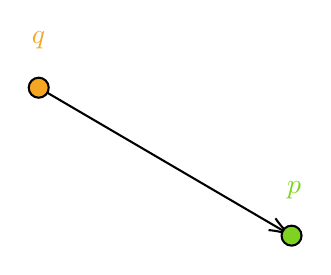
\begin{tikzpicture}[x=0.75pt,y=0.75pt,yscale=-1,xscale=1]
%uncomment if require: \path (0,300); %set diagram left start at 0, and has height of 300

%Straight Lines [id:da6747700231115574] 
\draw    (104.82,116.82) -- (224.91,187.09) ;
\draw [shift={(226.64,188.1)}, rotate = 210.34] [color={rgb, 255:red, 0; green, 0; blue, 0 }  ][line width=0.75]    (10.93,-3.29) .. controls (6.95,-1.4) and (3.31,-0.3) .. (0,0) .. controls (3.31,0.3) and (6.95,1.4) .. (10.93,3.29)   ;
%Shape: Circle [id:dp2346779756728088] 
\draw  [fill={rgb, 255:red, 126; green, 211; blue, 33 }  ,fill opacity=1 ] (221.82,188.1) .. controls (221.82,185.44) and (223.97,183.29) .. (226.64,183.29) .. controls (229.3,183.29) and (231.45,185.44) .. (231.45,188.1) .. controls (231.45,190.76) and (229.3,192.92) .. (226.64,192.92) .. controls (223.97,192.92) and (221.82,190.76) .. (221.82,188.1) -- cycle ;
%Shape: Circle [id:dp32683820972368327] 
\draw  [fill={rgb, 255:red, 245; green, 166; blue, 35 }  ,fill opacity=1 ] (100,116.82) .. controls (100,114.16) and (102.16,112) .. (104.82,112) .. controls (107.48,112) and (109.64,114.16) .. (109.64,116.82) .. controls (109.64,119.48) and (107.48,121.64) .. (104.82,121.64) .. controls (102.16,121.64) and (100,119.48) .. (100,116.82) -- cycle ;

% Text Node
\draw (100,88.4) node [anchor=north west][inner sep=0.75pt]  [color={rgb, 255:red, 245; green, 166; blue, 35 }  ,opacity=1 ]  {$q$};
% Text Node
\draw (223,160.4) node [anchor=north west][inner sep=0.75pt]  [color={rgb, 255:red, 126; green, 211; blue, 33 }  ,opacity=1 ]  {$p$};


\end{tikzpicture}
\end{FigureCenter} 


\end{example}

\begin{definition}[标量与向量的乘法]
    $$ \beta a=\left[\begin{array}{c}\beta a_{1} \\ \vdots \\ \beta a_{n}\end{array}\right] $$
\end{definition}

\begin{theorem}
    标量 \( \beta, \gamma \) 与向量 \( a 、 b \)进行乘法, 有如下性质:
    \begin{enumerate}
        \item 结合律: \( (\beta \gamma) a=\beta(\gamma a) \)
        \item 左分配律: \( (\beta+\gamma) a=\beta a+\gamma a \)
        \item 右分配律: \( \beta(a+b)=\beta a+\beta b \)
    \end{enumerate}
\end{theorem}

\begin{definition}[线性组合]
    对于向量 \( a_{1}, \ldots, a_{m} \) 和标量 \( \beta_{1}, \ldots, \beta_{m} \),
    $$ \beta_{1} a_{1}+\cdots+\beta_{m} a_{m} $$
    是向量的线性组合. \( \beta_{1}, \ldots, \beta_{m} \) 是该向量的\textit{系数}. 
\end{definition}



    \begin{theorem}
        对于任何向量 \( b \in \mathbb{R}^{n} \), 满足
    $$ b=b_{1} e_{1}+\cdots+b_{n} e_{n}, b=\left[\begin{array}{c}b_{1} \\ b_{2} \\ \vdots \\ b_{n}\end{array}\right] $$
    \end{theorem}
    
    $ \beta_{1}=\cdots=\beta_{m}=1 $时,线性组合是$a_1, \cdots, a_m$的和。

    $ \beta_{1}=\cdots=\beta_{m} = \frac{1}{m} $时,线性组合是$a_1, \cdots, a_m$的平均。

    When the coefficients sum to one, i.e., $ \beta_{1}+\cdots+\beta_{m}=1 $, the linear combination is called an \term{affine combination}. When the coefficients in an affine combination are nonnegative, it is called a \term{convex combination}, a \term{mixture}, or a \term{weighted average}. The coefficients in an affine or convex combination are sometimes given as percentages, which add up to $ 100 \% $.

\section{内积}

\begin{definition}[内积]
    在数域 \( \mathbb{R} \) 上的向量空间 \( V \), 定义函数 \( \langle\cdot,\cdot\rangle:V \times V \rightarrow \mathbb{R} \), 满足:

    \begin{enumerate}
        \item $ \langle{a}, {a}\rangle \geq 0, \forall {a} \in V $, 当且仅当 $a=0$ 时 $ \langle a, a\rangle=0 $.
        \item \( \langle\alpha {a}+\beta {b}, c\rangle=\alpha\langle{a}, c\rangle+\beta\langle{b}, c\rangle, \forall \alpha, \beta \in \mathbb{R} \), 且 \( {a}, {b}, c \in V \).
        \item \( \langle{a}, {b}\rangle=\langle{b}, {a}\rangle, \forall {a}, {b} \in V \).
    \end{enumerate}

    则称函数 \( \langle\cdot,\cdot\rangle:V \times V \rightarrow \mathbb{R} \)是内积. 
\end{definition}

\begin{example}[the inner product of two $ n $-vectors $ a, b $]
    在向量空间 \( \mathbb{R}^{n} \) 上,  计算两个向量对应项相乘之后求和函数
    $$ \langle a, b\rangle=a_{1} b_{1}+a_{2} b_{2}+\cdots+a_{n} b_{n}=a^{T}{b} $$

where \( a=\left[\begin{array}{c}a_{1} \\ a_{2} \\ \vdots \\ a_{n}\end{array}\right], b=\left[\begin{array}{c}b_{1} \\ b_{2} \\ \vdots \\ b_{n}\end{array}\right] \in \mathbb{R}^{n} \).
\end{example}

\begin{proof}
对于性质1
    $$\langle a, a\rangle=a^T a=a_{1} a_{1}+a_{2} a_{2}+\cdots+a_{n} a_{n}=\sum_{i=1}^{n} a_{i}^{2} \geq 0,$$

    $\langle a, a\rangle=0 则 a=0$.

    对于性质2
    $$\begin{aligned} \langle\alpha a+\beta {b}, {c}\rangle 
    & = (\alpha a+\beta {b})^T c 
    \\ &=\left(\alpha a_{1}+\beta b_{1}\right) c_{1}+\left(\alpha a_{2}+\beta b_{2}\right) c_{2}+\cdots+\left(\alpha a_{n}+\beta b_{n}\right) c_{n} 
    \\ &=\alpha \sum_{i=1}^{n} a_{i} c_{i}+\beta \sum_{i=1}^{n} b_{i} c_{i}
    \\ &=\alpha\langle a, c\rangle+\beta\langle b, c\rangle\end{aligned} $$

    对于性质3
    $$ \langle a, b\rangle=a^{{T}} b=b^{{T}} a=\langle b, a\rangle $$
\end{proof}

\begin{theorem}
    内积的性质:交换律、结合律、分配律. 

交换律(commutative): \( a^{T} b=b^{T} a \)

结合律(associative with scalar multiplication): \( (\gamma a)^{T} b=\gamma\left(a^{T} b\right) \)

分配律(distributive with vector addition): \( (a+b)^{T} c=a^{T} c+b^{T} c \)
\end{theorem}


\subsection{常用的内积等式}
\begin{corollary}[选出第$i$项]
    $$ e_{i}^{T} a=a_{i} $$
\end{corollary}

\begin{corollary}[向量每一项之和]
    $$ \mathbf{1}^{T} a=a_{1}+\cdots+a_{n} $$
\end{corollary}

\begin{corollary}[向量每一项的平方和]
    $$ a^{T} a=a_{1}^{2}+\cdots+a_{n}^{2} $$
\end{corollary}

\begin{corollary}[向量元素的平均值]
    $$ (\frac{\mathbf{1}}{n})^{T} a= \frac{a_{1}+\cdots+a_{n}}{n}  $$
\end{corollary}

\begin{corollary}[Selective sum]
    Let $ b $ be a vector all of whose entries are either 0 or 1 . Then $$ b^{T} a $$ is the sum of the elements in $ a $ for which $ b_{i}=1 $.
\end{corollary}

\begin{corollary}[Differencing]
    $$ \left(e_{i}-e_{j}\right)^{T} a=a_{i}-a_{j} $$
\end{corollary}

\begin{definition}[The sum of block vectors]
    If the vectors $ a $ and $ b $ are block vectors, and the corresponding blocks have the same sizes (in which case we say they \textit{conform}), then 

    $$ a^{T} b=\left[\begin{array}{c}a_{1} \\ \vdots \\ a_{k}\end{array}\right]^{T}\left[\begin{array}{c}b_{1} \\ \vdots \\ b_{k}\end{array}\right]=a_{1}^{T} b_{1}+\cdots+a_{k}^{T} b_{k} $$
\end{definition}


\section{Examples for Inner Product}

内积用途很广.

\begin{example}[计算同时出现的项目数]
   $$
a=(0,1,1,1,1,1,1), \quad b=(1,0,1,0,1,0,0)
$$
Here we have $ a^{T} b=2 $, which is the number of objects in both $ A $ and $ B $ (i.e., objects 3 and 5). 
\end{example}

\begin{example}[Weights, features, and score]
    When the vector $f$ represents a set of \textit{features} of
    an object, and $w$ is a vector of the same size (often called a \textit{weight vector}), the
    inner product $w^T f$ is the sum of the feature values, scaled (or weighted) by
    the weights, and is sometimes called a \textit{score}.

    Inner product $ w^{T} f=w_{1} f_{1}+w_{2} f_{2}+\cdots+w_{n} f_{n} $ is total score. 

\end{example}

\begin{example}[多项式]
    Suppose the $ n $-vector $ c $ represents the coefficients of a polynomial $ p $ of degree $ n-1 $ or less:

    $$ p(x)=c_{1}+c_{2} x+\cdots+c_{n-1} x^{n-2}+c_{n} x^{n-1} $$

    Let $t$ be a number, $ z=\left(1, t, t^{2}, \ldots, t^{n-1}\right) $  be the $n$-vector of powers
    of $t$. Then

    $$ c^{T} z=p(t) $$
\end{example}


\section{Cauchy-Schwartz Inequality}
\begin{theorem}[Cauchy-Schwartz Inequality]
    \label{thm:cauchy-schwartz=inequality}
    设 \( \langle \cdot,\cdot \rangle \) 是向量空间 \( V \) 上的内积, \( \forall x, y \in V \), 则有

    $$
|\langle x, y\rangle|^{2} \leq\langle x, x\rangle\langle y, y\rangle
$$

    当$x=-\lambda y$时,有$|\langle x, y\rangle|^{2}=\langle x, x\rangle\langle y, y\rangle$。
\end{theorem}

\begin{proof}
    令 $\lambda \in \mathbb{R}$, 则有 
    $$0 \leq\langle x+\lambda y, x+\lambda y\rangle=\langle x, x\rangle+\lambda\langle y, x\rangle+\lambda\langle x, y\rangle+\lambda^{2}\langle y, y\rangle=\langle x, x\rangle+2 \lambda\langle y, x\rangle+\lambda^{2}\langle y, y\rangle$$

则 
$$\lambda^{2}\langle y, y\rangle+2 \lambda\langle y, x\rangle+\langle x, x\rangle \geq 0, \forall \lambda \in \mathbb{R}$$

所以
$$
\begin{aligned}
&\nabla=(2\langle y, x\rangle)^{2}-4\langle y, y\rangle\langle x, x\rangle \leq 0 \\
&|\langle x, y\rangle|^{2} \leq\langle x, x\rangle\langle y, y\rangle
\end{aligned}
$$

当 $|\langle x, y\rangle|^{2}=\langle x, x\rangle\langle y, y\rangle$ 时, 有 $$\langle x, x\rangle^{2}+2 \lambda\langle y, x\rangle+\lambda^{2}\langle y, y\rangle=0$$

也即 $$\langle x+\lambda y, x+\lambda y\rangle=0$$

因此 $x+\lambda y=0$, 即 $x=-\lambda y$。
\end{proof}

\begin{theorem}[Cauchy-Schwarz 不等式的矩阵元素形式]

    $$\left(\sum_{i=1}^{n} u_{i} v_{i}\right)^{2} \leq\left(\sum_{i=1}^{n} u_{i}^{2}\right)\left(\sum_{i=1}^{n} v_{i}^{2}\right)$$
\end{theorem}

\begin{proof}
    The Cauchy-Schwarz inequality can be proved using only ideas from elementary algebra in this case. Consider the following quadratic polynomial in $x$
$$
0 \leq\left(u_{1} x+v_{1}\right)^{2}+\cdots+\left(u_{n} x+v_{n}\right)^{2}=\left(\sum_{i} u_{i}^{2}\right) x^{2}+2\left(\sum_{i} u_{i} v_{i}\right) x+\sum_{i} v_{i}^{2}
$$
Since it is nonnegative, it has at most one real root for $x$. Hence its discriminant is less than or equal to zero. That is,
$$
\Delta = \left(\sum_{i} u_{i} v_{i}\right)^{2}-\left(\sum_{i} u_{i}^{2}\right)\left(\sum_{i} v_{i}^{2}\right) \leq 0
$$
which yields the Cauchy-Schwarz inequality.
\end{proof}

\begin{corollary}[Cauchy-Schwarz不等式的等价形式]
    由Cauchy-Schwarz不等式
    $$
    |\langle x, y\rangle|^{2} \leq\langle x, x\rangle\langle y, y\rangle
    $$

    可以推得
    $$\begin{aligned}
        |\langle a,b \rangle| &\le \| a \|_2 \| b \|_2\\
        \langle a,b \rangle &\ge -\| a \|_2 \| b \|_2
    \end{aligned} $$
\end{corollary}


\section{浮点运算}

计算机以浮点格式存储(实)数值. 存储$n$维的向量需要$8n$字节进行存储。

基本的算术运算(加法, 乘法等)被称为浮点运算(flop). 

\begin{definition}[Floating point operation (flop)]
    the unit of complexity when comparing vector and matrix algorithms.

    1 flop $ = $ one basic arithmetic operation $ (+,-, *, /, \sqrt{,} \ldots) $ in $ \mathbf{R} $ or $ \mathbf{C} $.
\end{definition}

\begin{remark}
    This is a very simplified model of complexity of algorithms.

    \begin{itemize}
        \item we don't distinguish between the different types of arithmetic operations
        \item we don't distinguish between real and complex arithmetic
        \item we ignore integer operations (indexing, loop counters, ...)
        \item we ignore cost of memory access
    \end{itemize}
\end{remark}

算法或操作的时间复杂度:作为输入维数的函数所需要的浮点运算总数。算法复杂度通常以非常粗略地近似估算。(程序)执行时间的粗略估计:计算机速度/flops,目前的计算机大约是$1$Gflops/秒($10^9$flops/秒)。

\begin{definition}[Operation count (flop count)]
    Total number of operations in an algorithm. In linear algebra, it is typically a polynomial of the dimensions in the problem

\end{definition}
\begin{theorem}[通过浮点运算次数大致预测程序的运行时间]
    a crude predictor of run time of the algorithm.

    $$\text{run time}  \approx \frac{\text { number of operations (flops) }}{\text { computer speed (flops per second) }} $$
\end{theorem}

\begin{definition}[Dominant term]
    The highest-order term in the flop count.

\end{definition}

\begin{example}
    $$
\frac{1}{3} n^{3}+100 n^{2}+10 n+5 \approx \frac{1}{3} n^{3}
$$
\end{example}

\begin{definition}[Order]
    The power in the dominant term.
\end{definition}

\begin{example}
    $$
\frac{1}{3} n^{3}+10 n^{2}+100=\text { order } n^{3}
$$
\end{example}


\begin{corollary}
    假设有$n$维向量$x$和$y$

    \begin{itemize}
        \item $x+y$需要$n$次加法, 所以时间复杂度为 ($n$)flops. 
        \item $x^T y$ 需要$n$次乘法和$n - 1$次加法, 所以时间复杂度为$(2n - 1)$flops. 
        \item 对于$x^T y$, 通常将其时间复杂度简化为$2n$, 甚至为$n$. 
        \item 当$x$或$y$是稀疏的时候, 算法的实际运算时间会比理论时间更少. 
    \end{itemize}
\end{corollary}


\section{Complex numbers and Vectors}

\begin{definition}[Complex Numbers]
    $ x=\alpha+\mathrm{j} \beta $ with $ \alpha, \beta $ real scalars

    $ \mathrm{j}=\sqrt{-1} $ (more common notation is $ i $ or $ j $ ), $ \alpha $ is the \term{real} part of $ x $, denoted $ \operatorname{Re} x $, $ \beta $ is the \term{imaginary} part, denoted $ \operatorname{Im} x $
\end{definition}

\begin{definition}[Set of complex numbers]
    set of complex numbers is denoted $ \mathbf{C} $
\end{definition}

\begin{definition}[Modulus]
    modulus (absolute value, magnitude): $$ |x|=\sqrt{(\operatorname{Re} x)^{2}+(\operatorname{Im} x)^{2}} $$
\end{definition}

\begin{definition}[Conjugate]
    $$ \bar{x}=\operatorname{Re} x-\mathrm{j} \operatorname{Im} x $$
\end{definition}

\begin{theorem}
    $$ \operatorname{Re} x=\frac{x+\bar{x}}{2} $$
\end{theorem}

\begin{theorem}
    $$ \operatorname{Im} x=\frac{x-\bar{x}}{2 \mathrm{j}} $$
\end{theorem}

\begin{theorem}
    $$ |x|^{2}=\bar{x} x $$
\end{theorem}

\subsection{Polar representation}

\begin{theorem}
    nonzero complex number $ x=\operatorname{Re} x+\mathrm{j} \operatorname{Im} x $ can be written as
$$
x=|x|(\cos \theta+\mathrm{j} \sin \theta)=|x| e^{\mathrm{j} \theta}
$$

$ \theta \in[0,2 \pi) $ is the \term{argument} (\term{phase angle}) of $ x $ (notation: $ \arg x $ ). $ e^{\mathrm{j} \theta} $ is complex exponential.
\end{theorem}

\begin{theorem}[Euler's formula]
    $ e^{\mathrm{j} \theta}=\cos \theta+\mathrm{j} \sin \theta $
\end{theorem}

\begin{FigureCenter}{Complex Numbers}
    

\tikzset{every picture/.style={line width=0.75pt}} %set default line width to 0.75pt        

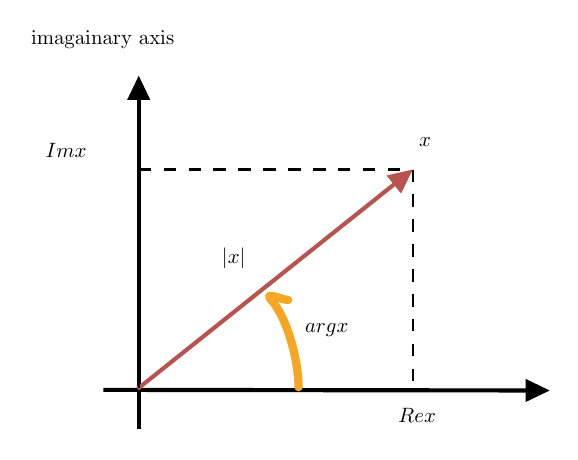
\begin{tikzpicture}[x=0.75pt,y=0.75pt,yscale=-1,xscale=1]
%uncomment if require: \path (0,300); %set diagram left start at 0, and has height of 300

%Straight Lines [id:da4158839935279788] 
\draw [line width=1.5]    (267,233) -- (478,233.3) ;
\draw [shift={(482,233.3)}, rotate = 180.08] [fill={rgb, 255:red, 0; green, 0; blue, 0 }  ][line width=0.08]  [draw opacity=0] (11.61,-5.58) -- (0,0) -- (11.61,5.58) -- cycle    ;
%Straight Lines [id:da5390398615537384] 
\draw [line width=1.5]    (284,252) -- (284,85.68) ;
\draw [shift={(284,81.68)}, rotate = 90] [fill={rgb, 255:red, 0; green, 0; blue, 0 }  ][line width=0.08]  [draw opacity=0] (11.61,-5.58) -- (0,0) -- (11.61,5.58) -- cycle    ;
%Straight Lines [id:da928526944402611] 
\draw [color={rgb, 255:red, 184; green, 84; blue, 80 }  ,draw opacity=1 ][fill={rgb, 255:red, 184; green, 84; blue, 80 }  ,fill opacity=1 ][line width=1.5]    (283.5,232.5) -- (412.87,129.33) ;
\draw [shift={(416,126.84)}, rotate = 141.43] [fill={rgb, 255:red, 184; green, 84; blue, 80 }  ,fill opacity=1 ][line width=0.08]  [draw opacity=0] (11.61,-5.58) -- (0,0) -- (11.61,5.58) -- cycle    ;
%Shape: Rectangle [id:dp5932303428508245] 
\draw  [dash pattern={on 4.5pt off 4.5pt}] (284,126.84) -- (416,126.84) -- (416,233.5) -- (284,233.5) -- cycle ;
%Shape: Free Drawing [id:dp3532268261143874] 
\draw  [color={rgb, 255:red, 245; green, 166; blue, 35 }  ,draw opacity=1 ][line width=3] [line join = round][line cap = round] (361,231.7) .. controls (361,218.56) and (355.2,196.89) .. (347,188.7) ;
%Shape: Free Drawing [id:dp6391532692612814] 
\draw  [color={rgb, 255:red, 245; green, 166; blue, 35 }  ,draw opacity=1 ][line width=3] [line join = round][line cap = round] (347,187.7) .. controls (350.61,187.7) and (353.29,189.7) .. (356,189.7) ;


% Text Node
\draw (238,113) node [anchor=north west][inner sep=0.75pt]  [xscale=0.75,yscale=0.75] [align=left] {$\displaystyle \operatorname{Im} x$};
% Text Node
\draw (408,241) node [anchor=north west][inner sep=0.75pt]  [xscale=0.75,yscale=0.75] [align=left] {$\displaystyle \operatorname{Re} x$};
% Text Node
\draw (231,59) node [anchor=north west][inner sep=0.75pt]  [xscale=0.75,yscale=0.75] [align=left] {imagainary axis};
% Text Node
\draw (418,110.4) node [anchor=north west][inner sep=0.75pt]  [xscale=0.75,yscale=0.75]  {$x$};
% Text Node
\draw (323,163.4) node [anchor=north west][inner sep=0.75pt]  [xscale=0.75,yscale=0.75]  {$| x| $};
% Text Node
\draw (363,200) node [anchor=north west][inner sep=0.75pt]  [xscale=0.75,yscale=0.75] [align=left] {$\displaystyle \operatorname{arg} x$};


\end{tikzpicture}
\end{FigureCenter}

\subsection{Complex vector}

\begin{definition}[vector with complex elements]
    $ a=\alpha+\mathrm{j} \beta $ with $ \alpha, \beta $ real vectors
\end{definition}

\begin{definition}[real and imaginary part, conjugate of complex numbers]
    real and imaginary part, conjugate are defined componentwise:

$$
\begin{aligned}
\operatorname{Re} a &=\left(\operatorname{Re} a_{1}, \operatorname{Re} a_{2}, \ldots, \operatorname{Re} a_{n}\right) \\
\operatorname{Im} a &=\left(\operatorname{Im} a_{1}, \operatorname{Im} a_{2}, \ldots, \operatorname{Im} a_{n}\right) \\
\bar{a} &=\operatorname{Re} a-\mathrm{j} \operatorname{Im} a
\end{aligned}
$$
\end{definition}

\begin{definition}[ set of complex $n$-vectors]
    $$ \mathbf{C}^{n} $$
\end{definition}

\begin{definition}
    $$ a+b=\left[\begin{array}{c}a_{1}+b_{1} \\ a_{2}+b_{2} \\ \vdots \\ a_{n}+b_{n}\end{array}\right], \quad \gamma a=\left[\begin{array}{c}\gamma a_{1} \\ \gamma a_{2} \\ \vdots \\ \gamma a_{n}\end{array}\right], \quad a \circ b=\left[\begin{array}{c}a_{1} b_{1} \\ a_{2} b_{2} \\ \vdots \\ a_{n} b_{n}\end{array}\right] $$
\end{definition}

\begin{definition}[Complex inner product]
    the inner product of complex $ n $-vectors $ a, b $ is defined as
$$
b^{H} a=\bar{b}_{1} a_{1}+\bar{b}_{2} a_{2}+\cdots+\bar{b}_{n} a_{n}
$$
\end{definition}

other notation: $ \langle a, b\rangle,(a \mid b), \ldots $.

for real vectors, reduces to real inner product $ b^{T} a $.

for complex $ n $-vectors $ a, b, c $ and complex scalars $ \gamma $

$a^H a$有如下性质:
\begin{theorem}
    $ a^{H} a \geq 0 $ : follows from
$$
\begin{aligned}
a^{H} a &=\bar{a}_{1} a_{1}+\bar{a}_{2} a_{2}+\cdots+\bar{a}_{n} a_{n} \\
&=\left|a_{1}\right|^{2}+\left|a_{2}\right|^{2}+\cdots+\left|a_{n}\right|^{2}
\end{aligned}
$$

\end{theorem}

\begin{theorem}
    $$ a^{H} a=0 \text{ only if } a=0 $$
\end{theorem}

\begin{theorem}
    $$ b^{H} a=\overline{a^{H} b} $$
\end{theorem}

\begin{theorem}
    $$ (\gamma b)^{H} a=\bar{\gamma}\left(b^{H} a\right) $$
\end{theorem}

\begin{theorem}
    $$ (b+c)^{H} a=b^{H} a+c^{H} a $$
\end{theorem}

\begin{theorem}
    $$ b^{H}(a+c)=b^{H} a+b^{H} c $$
\end{theorem}

\begin{theorem}
    $$ b^{H}(\gamma a)=\gamma\left(b^{H} a\right) $$
\end{theorem}
\chapter{Linear Function}

\section{Linear Function}

\begin{definition}[Linear Function]
    $f: \mathbb{R}^{n} \rightarrow \mathbb{R}$是一个将$n$维向量映射成数的函数. 

    线性函数 $ f $ 满足以下两个性质 $ \left(k \in \mathbb{R}, x, y \in \mathbb{R}^{n}\right) $ :

    \begin{itemize}
        \item 齐次性(homogeneity): $ f(k x)=k f(x) $
        \item 叠加性(Additivity): $ f(x+y)=f(x)+f(y) $
    \end{itemize}
\end{definition}

\begin{example}
    求平均值: $ f(x)=\frac{1}{n} \sum_{i=1}^{n} x_{i} $ 为线性函数. 
\end{example}

\begin{example}
    求最大值: $ f(x)=\max \left\{x_{1}, x_{2}, \ldots, x_{n}\right\} $ 并不是线性函数. 
\end{example}

\begin{proof}
   令 $ x=(1,-1), y=(-1,1), \alpha=0.5, \beta=0.5 $, 
   有 $$ f(\alpha x+\beta y)=0 \neq \alpha f(x)+\beta f(y)=1 $$

    但是
   $$ \begin{aligned} f(x+y) 
    &=\max \left\{x_{1}+y_{1}, x_{2}+y_{2}, \ldots, x_{n}+y_{n}\right\} 
    \\ & \leq \max \left\{x_{1}, x_{2}, \ldots, x_{n}\right\}+\max \left\{y_{1}, y_{2}, \ldots, y_{n}\right\} 
    \\ & \leq f(x)+f(y) \end{aligned} $$

    不满足线性函数的定义
\end{proof}

\begin{theorem}
        a function $ f: \mathbf{R}^{n} \rightarrow \mathbf{R} $ is linear if the \term{superposition property} (叠加原理)
    $$
    f(\alpha x+\beta y)=\alpha f(x)+\beta f(y)
    $$
    holds for all $ n $-vectors $ x, y $ and all scalars $ \alpha, \beta $.
    
\end{theorem}

In fact it says a lot. On the left-hand side, the term $ \alpha x+\beta y $ involves scalar-vector multiplication and vector addition. On the right-hand side, $ \alpha f(x)+\beta f(y) $ involves ordinary scalar multiplication and scalar addition.

\begin{corollary}
    设 $ \alpha_{1, \ldots,} \alpha_{m} \in \mathbb{R}, u_{1}, \ldots, u_{m} \in \mathbb{R}^{n} $, 则线性函数 $ f $ 满足

    $$ \begin{aligned} f\left(\alpha_{1} u_{1}+\alpha_{2} u_{2}+\ldots+\alpha_{m} u_{m}\right) &=f\left(\alpha_{1} u_{1}\right)+f\left(\alpha_{2} u_{2}+\ldots+\alpha_{m} u_{m}\right) \\ &=\alpha_{1} f\left(u_{1}\right)+f\left(\alpha_{2} u_{2}+\ldots+\alpha_{m} u_{m}\right) \\ &=\alpha_{1} f\left(u_{1}\right)+\alpha_{2} f\left(u_{2}\right)+\ldots+\alpha_{m} f\left(u_{m}\right) \end{aligned} $$
\end{corollary}

\begin{definition}[内积函数 (inner product function)]
    对于$n$维向量 $ a $,满足以下形式的函数$ f: \mathbf{R}^{n} \rightarrow \mathbf{R} $被称为内积函数

    $$ f(x)=a^{T} x=a_{1} x_{1}+a_{2} x_{2}+\ldots+a_{n} x_{n} $$
\end{definition}

上述 $ f(x) $ 可以看作是每项 $ x_{\mathrm{i}} $ 的加权之和. 

\begin{example}
    $ f(x)=\frac{1}{3}\left(x_{1}+x_{2}+x_{3}\right) $ is linear: $ f(x)=a^{T} x $ with $ a=\left(\frac{1}{3}, \frac{1}{3}, \frac{1}{3}\right) $
\end{example}

\begin{example}
    $ f(x)=-x_{1} $ is linear: $ f(x)=a^{T} x $ with $ a=(-1,0,0) $
\end{example}

\begin{example}
    $ f(x)=\max \left\{x_{1}, x_{2}, x_{3}\right\} $ is not linear.
\end{example}

\begin{proof}
    Superposition does not hold for
$$
x=\left[\begin{array}{l}
1 \\
0 \\
0
\end{array}\right], \quad y=\left[\begin{array}{l}
0 \\
0 \\
0
\end{array}\right], \quad \alpha=-1, \quad \beta=1
$$
we have $ f(x)=1, f(y)=0 $,
$$
f(\alpha x+\beta y)=0 \neq \alpha f(x)+\beta f(y)=-1
$$
\end{proof}

\begin{theorem}
    所有的内积函数都是线性的.

    $$
a^{T}(\alpha x+\beta y)=\alpha\left(a^{T} x\right)+\beta\left(a^{T} y\right)
$$
holds for all scalars $ \alpha, \beta $ and all $ n $-vectors $ x, y $.
\end{theorem}

\begin{proof}
    $$ \begin{aligned} f(\alpha x+\beta y) &=a^{T}(\alpha x+\beta y) \\ &=a^{T}(\alpha x)+a^{T}(\beta y) \\ &=\alpha\left(a^{T} x\right)+\beta\left(a^{T} y\right) \\ &=\alpha f(x)+\beta f(y) \end{aligned} $$
\end{proof}


\begin{theorem}
    所有的线性函数都是内积函数.

    $$ \begin{aligned} f(x) &=f\left(x_{1} e_{1}+x_{2} e_{2}+\ldots+x_{n} e_{n}\right) \\ &=x_{1} f\left(e_{1}\right)+x_{2} f\left(e_{2}\right)+\ldots+x_{n} f\left(e_{n}\right) \end{aligned} $$
\end{theorem}

\begin{proof}
    假设 $ f: \mathbb{R}^{n} \rightarrow \mathbb{R} $ 是线性函数, 那么可用 $ f(x)=a^{T} x $ 来表示, $ a $ 为常量.

    $$ \begin{aligned} f(x) &=f\left(x_{1} e_{1}+x_{2} e_{2}+\ldots+x_{n} e_{n}\right) \\ &=x_{1} f\left(e_{1}\right)+x_{2} f\left(e_{2}\right)+\ldots+x_{n} f\left(e_{n}\right) \\ & = a^Tx \quad (a = ( f\left(e_{1}\right), f\left(e_{2}\right), \ldots, f\left(e_{n}\right) )) \end{aligned} $$
\end{proof}

\begin{definition}[Inner product representation of $ f $]
    Suppose $ f $ is a scalar-valued function of $ n $-vectors, and is linear  holds for all $ n $-vectors $ x, y $, and all scalars $ \alpha, \beta $. Then there is an $ n $-vector $ a $ such that $ f(x)=a^{T} x $ for all $ x $. We call $ a^{T} x $ the inner product representation of $ f $.
\end{definition}

\section{Affine Function}


\begin{definition}[仿射函数 (affine function)]
    其一般形式为 $ f(x)=a^{T} x+{b} $, 其中 $ a \in \mathbb{R}^{n}, b \in \mathbb{R} $ 为标量. 

    
        for fixed $ a \in \mathbf{R}^{n}, b \in \mathbf{R} $, define a function $ f: \mathbf{R}^{n} \rightarrow \mathbf{R} $ by
    $$
    f(x)=a^{T} x+b=a_{1} x_{1}+a_{2} x_{2}+\cdots+a_{n} x_{n}+b
    $$
    
    i.e., an inner-product function plus a constant (offset)
    
\end{definition}

\begin{theorem}
    函数 $ f: \mathbb{R}^{n} \rightarrow \mathbb{R} $ 为仿射函数需要满足

$$ f(\alpha x+\beta y)=\alpha f(x)+\beta f(y), \alpha+\beta=1, \alpha, \beta \in \mathbb{R}, x, y \in \mathbb{R}^{n} $$
\end{theorem}

\begin{corollary}
    If $ f $ is affine, then
$$
f\left(\alpha_{1} u_{1}+\alpha_{2} u_{2}+\cdots+\alpha_{m} u_{m}\right)=\alpha_{1} f\left(u_{1}\right)+\alpha_{2} f\left(u_{2}\right)+\cdots+\alpha_{m} f\left(u_{m}\right)
$$
for all $ n $-vectors $ u_{1}, \ldots, u_{m} $ and all scalars $ \alpha_{1}, \ldots, \alpha_{m} $ with
$$
\alpha_{1}+\alpha_{2}+\cdots+\alpha_{m}=1
$$
\end{corollary}



\begin{theorem}[restricted superposition property]
    Any function of this type is affine.
    
    $$ f(\alpha x+\beta y)=\alpha f(x)+\beta f(y) $$
\end{theorem}

\begin{proof}
    If $ \alpha+\beta=1 $ then
    $$ \begin{aligned} f(\alpha x+\beta y) &=a^{T}(\alpha x+\beta y)+b \\ &=\alpha a^{T} x+\beta a^{T} y+(\alpha+\beta) b \\ &=\alpha\left(a^{T} x+b\right)+\beta\left(a^{T} y+b\right) \\ &=\alpha f(x)+\beta f(y) \end{aligned} $$

    (In the second line we use $\alpha + \beta = 1$.)

\end{proof}

\begin{corollary}
    This restricted superposition property for affine functions is useful in showing that a function $ f $ is not affine: We find vectors $ x, y $, and numbers $ \alpha $ and $ \beta $ with $ \alpha+\beta=1 $, and verify that $ f(\alpha x+\beta y) \neq \alpha f(x)+\beta f(y) . $ This shows that $ f $ cannot be affine.
\end{corollary}

\begin{theorem}
    every affine function can be written as $ f(x)=a^{T} x+b $ with:
$$
\begin{array}{l}
a=\left(f\left(e_{1}\right)-f(0), f\left(e_{2}\right)-f(0), \ldots, f\left(e_{n}\right)-f(0)\right) \\
b=f(0)
\end{array}
$$

\end{theorem}


\section{泰勒展开}

\begin{definition}[函数$f$第$i$个分量的一阶偏导数]
    假设 $ f: \mathbb{R}^{n} \rightarrow \mathbb{R} $ , 函数 $ f $ 在 $ z $ 点可微

    $$ \begin{aligned} \frac{\partial f}{\partial z_{i}}(z) &=\lim _{t \rightarrow 0} \frac{f\left(z_{1}, \cdots, z_{i-1}, z_{i}+t, z_{i+1}, \cdots, z_{n}\right)-f(z)}{t} \\ &=\lim _{t \rightarrow 0} \frac{f\left(z+t e_{i}\right)-f(z)}{t} \end{aligned} $$
\end{definition}

\begin{definition}[$f$在点$z$的梯度]
    $$ \nabla f(z)=\left[\begin{array}{c}\frac{\partial f}{\partial z_{1}}(z) \\ \vdots \\ \frac{\partial f}{\partial z_{n}}(z)\end{array}\right] $$
\end{definition}

\begin{definition}[Taylor's Approximation]
    假设 $ f: \mathbb{R}^{n} \rightarrow \mathbb{R} $ , 函数 $ f $ 在 $ z $ 点充分光滑, 即处处可导.

    $f(x)$在$z$附近的泰勒展开是

    $$\begin{aligned} f(x)&=f(z)+\frac{\partial f}{\partial x_{1}}(z)\left(x_{1}-z_{1}\right)+\frac{\partial f}{\partial x_{2}}(z)\left(x_{2}-z_{2}\right)+\cdots+\frac{\partial f}{\partial x_{n}}(z)\left(x_{n}-z_{n}\right) 
    \\ & +\frac{1}{2 !} \sum_{j=1}^{n} \sum_{i=1}^{n} \frac{\partial f^{2}}{\partial x_{i} \partial x_{j}}(z)\left(x_{i}-z_{i}\right)\left(x_{\mathrm{j}}-z_{j}\right)+\cdots \end{aligned}$$
\end{definition}


\begin{definition}[一阶泰勒公式]
    假设$ f: \mathbb{R}^{n} \rightarrow \mathbb{R} $, 函数$f$在$z$点可导

    $$ \hat{f}(x)=f(z)+\frac{\partial f}{\partial x_{1}}(z)\left(x_{1}-z_{1}\right)+\ldots+\frac{\partial f}{\partial x_{1}}(z)\left(x_{n}-z_{n}\right) $$
\end{definition}

当$x$非常接近$z$时, $ \hat{f}(x) $ 也非常接近 $ f(z) $.  
$ \hat{f}(x) $ 是关于 $ x $ 的一个仿射函数. 

\begin{corollary}[一阶泰勒公式的内积形式]
    $$ \hat{f}(x)=f(z)+\nabla f(z)^{T}(x-z) \quad (\nabla f(z)=\left[\begin{array}{c}\frac{\partial f}{\partial x_{1}}(z) \\ \vdots \\ \frac{\partial f}{\partial x_{n}}(z)\end{array}\right]) $$

    the $ n $-vector $ \nabla f(z) $ is called the \term{gradient} of $ f $ at $ z $.
\end{corollary} 

一维时, $ \hat{f}(x)=f(z)+f^{\prime}(z)(x-z) $.

\begin{example}
    $$ f(x)=x_{1}-3 x_{2}+e^{2 x_{1}+x_{2}-1} $$

    $$ \nabla f(x)=\left[\begin{array}{l}\frac{\partial f}{\partial x_{1}}(x) \\ \frac{\partial f}{\partial x_{2}}(x)\end{array}\right]=\left[\begin{array}{l}1+2 e^{2 x_{1}+x_{2}-1} \\ -3+e^{2 x_{1}+x_{2}-1}\end{array}\right] $$

    函数 $ f $ 在 0 点的一阶泰勒公式为:
    $$ \hat{f}(x)=f(0)+\nabla f(0)^{T}(x-0)=e^{-1}+\left(1+2 e^{-1}\right) x_{1}+\left(-3+e^{-1}\right) x_{2} $$
\end{example}

\section{高阶泰勒公式}

    泰勒公式利用多项式在一点附近逼近函数.
    


\begin{corollary}[$n$阶泰勒多项式]
    $$ \begin{aligned} P_{n}(x) &=f\left(x_{0}\right)+f^{\prime}\left(x_{0}\right)\left(x-x_{0}\right)+\frac{f^{\prime \prime}\left(x_{0}\right)}{2 !}\left(x-x_{0}\right)^{2} +\cdots+\frac{f^{(n)}\left(x_{0}\right)}{n !}\left(x-x_{0}\right)^{n} \end{aligned} $$
    where $a_{n}=\frac{f^{(n)}\left(x_{0}\right)}{n !} $
\end{corollary}

\begin{corollary}[对于高阶余项的公式]
    带拉格朗日余项的泰勒公式
    $$ \begin{aligned} f(x) &=f\left(x_{0}\right)+f^{\prime}\left(x_{0}\right)\left(x-x_{0}\right)+\frac{f^{\prime \prime}\left(x_{0}\right)}{2 !}\left(x-x_{0}\right)^{2} \\ &+\cdots+\frac{f^{(n)}\left(x_{0}\right)}{n !}\left(x-x_{0}\right)^{n}+\frac{f^{(n+1)}(\xi)}{(n+1) !}\left(x-x_{0}\right)^{n+1} \end{aligned} $$

    $ R_{n}(x)=\frac{f^{(n+1)}(\xi)}{(n+1) !}\left(x-x_{0}\right)^{n+1}\left(\xi\right. $ 在 $ x_{0} $ 与 $ x  $ 之间 $ ) $
\end{corollary}

\begin{corollary}[麦克劳林(Maclaurin)公式]在零点展开麦克劳林(Maclaurin)公式
    $$ \begin{aligned} f(x)=& f(0)+f^{\prime}(0) x+\frac{f^{\prime \prime}(0)}{2 !} x^{2}+\cdots+\frac{f^{(n)}(0)}{n !} x^{n} +\frac{f^{(n+1)}(\theta x)}{(n+1) !} x^{n+1} &(0<\theta<1) \end{aligned} $$
    
\end{corollary}


\section{Regression Model}
\begin{definition}[Regression Model]
    回归模型(regression model)为关于$x$的仿射函数
    $$ \hat{y}=x^{T} \beta+v $$

    $x$是\textit{特征向量(feature vector)}, 它的元素$x_i$称为\textit{回归元(regressors)}. $n$维向量 $ \beta $ 是\textit{权重向量(weight vector)}. 标量 $ v $ 是\textit{偏移量(offset)}. 标量 $ \hat{y} $ 是\textit{预测值(prediction)}. 表示某个实际结果或因变量, 用$y$表示. 
\end{definition}

\begin{example}
    $$ \sin x= x-\frac{x^{3}}{3 !}+\frac{x^{5}}{5 !}-\cdots+(-1)^{k-1} \frac{x^{2 k-1}}{(2 k-1) !}+\frac{\sin \left[\xi+(2 k+1) \frac{\pi}{2}\right]}{(2 k+1) !} x^{2 k+1} $$

    一次逼近: $  \sin x \approx x $

    三次逼近: $  \sin x \approx x-\frac{x^{3}}{3 !} $
\end{example}

\begin{proof}
    $$ f(x)=P_{n}(x)+R_{n}(x) $$
    
    $ P_{n}(x)=a_{0}+a_{1}\left(x-x_{0}\right)+a_{2}\left(x-x_{0}\right)^{2}+\cdots+a_{n}\left(x-x_{0}\right)^{n}  $

    $ R_{n}(x)=o\left(x-x_{0}\right)^{n} $

    $ f(x) \approx P_{n}(x) $

    $\therefore  P_{n}\left(x_{0}\right)=f\left(x_{0}\right) $,
    $ P_{n}^{\prime}\left(x_{0}\right)=f^{\prime}\left(x_{0}\right) $,
    $ P_{n}^{\prime \prime}\left(x_{0}\right)=f^{\prime \prime}\left(x_{0}\right) $,
    $ \cdots  $,
    $ P_{n}^{(n)}\left(x_{0}\right)=f^{(n)}\left(x_{0}\right) $

    要求 $ P_{n}\left(x_{0}\right)=f\left(x_{0}\right) \Rightarrow  a_{0}=f\left(x_{0}\right)  $

    $$ P_{n}^{\prime}(x)=a_{1}+2 a_{2}\left(x-x_{0}\right)+\cdots+n a_{n}\left(x-x_{0}\right)^{n-1} \Rightarrow  a_{1}=f^{\prime}\left(x_{0}\right)  $$

    依此类推. $a_{n}=\frac{f^{(n)}\left(x_{0}\right)}{n !} $
\end{proof}
\chapter{Norm and Distance}

\section{Vector Norm}

\begin{definition}[Vector Norm]
    在向量空间中存在一个函数 $ \|\cdot\|: \mathbb{R}^{n} \rightarrow \mathbb{R} $, 且满足以下条件

\begin{itemize}
    \item 齐次性: $ \|\alpha x\|=|\alpha|\|x\|, \quad \alpha \in \mathbb{R} $ 且 $ x \in \mathbb{R}^{n} $;
    \item 三角不等式: $ \|x+y\| \leq\|x\|+\|y\|, \quad x, y \in \mathbb{R}^{n} $;
    \item 非负性: $ \|x\| \geq {0}, \boldsymbol{x} \in \mathbb{R}^{n} $ 且 $ \|\boldsymbol{x}\|=0 \Leftrightarrow \boldsymbol{x}=0 $;
\end{itemize}
则称$\|\cdot\|$为向量范数. 
\end{definition}

\begin{example}[$ \ell_{1} $-范数(曼哈顿范数,  Manhattan norm)]
    $$ \|x\|_{1}=\left|x_{1}\right|+\left|x_{2}\right|+\ldots+\left|x_{n}\right| \quad x, y \in \mathbb{R}^{n}, \alpha \in \mathbb{R} $$
\end{example}

\begin{proof}
    $$ \|\alpha x\|_{1}=\left|\alpha x_{1}\right|+\left|\alpha x_{2}\right|+\cdots+\left|\alpha x_{n}\right|=|\alpha|\|x\|_{1} \geq 0 $$

    $$ \|x+y\|_{1}=\left|x_{1}+y_{1}\right|+\cdots+\left|x_{n}+y_{n}\right| \leq\left|x_{1}\right|+\left|y_{1}\right|+\cdots+\left|x_{n}\right|+\left|y_{n}\right|=\|x\|_{1}+\|y\|_{1} $$
\end{proof}

\begin{example}[$ \ell_{2} $-范数(欧几里得范数, Euclidean norm)]
    $$ \|x\|_{2}=\sqrt{\left(x_{1}^{2}+x_{2}^{2}+\cdots+x_{n}^{2}\right)}=\sqrt{x^{T} x}=(\langle x, x\rangle)^{\frac{1}{2}} $$
\end{example}

\begin{proof}
    $$ \|\alpha x\|_{2}=(\langle\alpha x, \alpha x\rangle)^{\frac{1}{2}}=|\alpha|(\langle x, x\rangle)^{\frac{1}{2}}=|\alpha|\|x\|_{2} $$
    
    $$\begin{aligned} \|x+y\|_{2}^{2}&=\langle x+y, x+y\rangle=\langle x, x\rangle+\langle x, y\rangle+\langle y, x\rangle+\langle y, y\rangle  \\
    &=\|x\|_{2}^{2}+2\langle x, y\rangle+\|y\|_{2}^{2} \leq\|x\|_{2}^{2}+2\|x\|_{2}\|y\|_{2}+\|y\|_{2}^{2}\\
    &=\left(\|x\|_{2}+\|y\|_{2}\right)^{2} \end{aligned}$$

    $$ \|x+y\|_{2} \leq\|x\|_{2}+\|y\|_{2} $$
\end{proof}

\begin{corollary}[柯西—施瓦茨不等式]
    $$ |\langle x, y\rangle|^{2} \leq\langle x, x\rangle\langle y, y\rangle=\|x\|_{2}^{2}\|y\|_{2}^{2} $$
\end{corollary}

\begin{definition}[$ \ell_{\infty} $-范数]
    $$ \|x\|_{\infty}=\max _{1 \leq i \leq n}\left|x_{i}\right|, x \in \mathbb{R}^{n} $$
\end{definition}

\begin{proof}
    $$ \begin{aligned} \max _{1 \leq i \leq n}\left|x_{i}\right| 
        &\leq \left(\left|x_{1}\right|^{p}+\cdots+\left|x_{i}\right|^{p}+\cdots+\left|x_{n}\right|^{p}\right)^{1 / p} \\
        &\leq \left(n \max _{1 \leq i \leq n}\left|x_{i}\right|^{p}\right)^{1 / p}\\
        &  =n^{1 / p} \max _{1 \leq i \leq n}\left|x_{i}\right| \\ &\rightarrow \max _{1 \leq i \leq n}\left|x_{i}\right| \quad(p \rightarrow \infty)\end{aligned}
    $$
\end{proof}

\begin{definition}[$ \ell_{\mathrm{p}} $-范数]
    $$ \|x\|_{p}=\left(x_{1}^{\mathrm{p}}+x_{2}^{p}+\cdots+x_{n}^{p}\right)^{\frac{1}{p}}, \quad x \in \mathbb{R}^{n}, p \ge 1 $$

    $ \ell_{1} $ 范数 $ \|x\|_{1}$,$ \ell_{2} $-范数 $ \|x\|_{2} $, $ \ell_{\infty} $-范数是 $ \ell_{p} $-范数的特例. 
\end{definition}

证明可以使用以下两条不等式

\begin{theorem}[Minkowshi Inequality]
    $$ \left(\sum_{i=1}^{n}\left|x_{i}+y_{i}\right|^{p}\right)^{\frac{1}{p}} \leq\left(\sum_{i=1}^{n}\left|x_{i}\right|^{p}\right)^{\frac{1}{p}}+\left(\sum_{i=1}^{n}\left|y_{i}\right|^{p}\right)^{\frac{1}{p}}, p \geq 1, x, y \in \mathbb{R}^{n} $$
\end{theorem}

\begin{theorem}[Hölder Inequality]
    $$ \sum_{i=1}^{n}\left|x_{i} y_{i}\right| \leq\left(\sum_{i=1}^{n}\left|x_{i}\right|^{p}\right)^{1 / p}\left(\sum_{i=1}^{n}\left|y_{i}\right|^{q}\right)^{1 / q}, \frac{1}{p}+\frac{1}{q}=1,1<p, q<\infty $$
\end{theorem}

\section{Root Mean Square Value (RMS)}

\begin{definition}[向量 $ x $的均方值 (mean-square value)]
    向量 $ x \in \mathbb{R}^n $的均方值 (mean-square value)

    $$ \frac{x_{1}^{2}+x_{2}^{2}+\cdots+x_{n}^{2}}{n}=\frac{\|x\|_{2}^{2}}{n} $$
\end{definition}

\begin{definition}[n维向量 $ x $ 的均方根(root-mean-square value, RMS)]
    $$ \operatorname{rms}(x)=\sqrt{\frac{x_{1}^{2}+x_{2}^{2}+\cdots+x_{n}^{2}}{n}}=\frac{\|x\|_{2}}{\sqrt{n}} $$
\end{definition}

$ \operatorname{rms}(x) $ 给出了 $ \left|x_{i}\right| $ 的 “典型" (typical)值. 例如, $ \mathrm{rms}(\mathbf{1})=1 $ (与$n$无关). 均方根(RMS)值对于比较不同长度的向量大小是比较有用的. 

\section{Chebyshev's Inequality}

\begin{theorem}[Chebyshev's Inequality]
$$
\begin{aligned}
    P(|X-\mu| \ge \varepsilon) \le \frac{\sigma^2}{\varepsilon^2}
\end{aligned}
$$

$$
 P(|X-\mu| < \varepsilon) \ge 1 - \frac{\sigma^2}{\varepsilon^2}
$$
\end{theorem}

\begin{theorem}[Chebyshev's Inequality]
    假设$k$为向量 $ x $ 分量满足条件 $ \left|x_{i}\right| \geq a $ 的个数, 即 $ x_{i}^{2} \geq a^{2} $ 的个数. 

    因此: $ \|x\|_{2}^{2}=x_{1}^{2}+x_{2}^{2}+\cdots+x_{n}^{2} \geq k a^{2} $

    将 $ a^{2} $ 移项, 可得到 $ k \leq \frac{\|x\|_{2}^{2}}{a^{2}} $

    满足 $ \left|x_{i}\right| \geq a $ 的 $ x_{i} $ 数量不会超过 $ \frac{\|\| \|_{2}^{2}}{a^{2}} $
\end{theorem}

\begin{corollary}[Chebyshev's Inequality Using RMS]
    $$ \operatorname{rms}(x)=\sqrt{\frac{x_{1}^{2}+x_{2}^{2}+\cdots+x_{n}^{2}}{n}}=\frac{\|x\|_{2}}{\sqrt{n}} $$

    $ \left|x_{i}\right| \geq a $ 的项数占整体的比例不会超过 $ \left(\frac{\operatorname{rms}(x)}{a}\right)^{2} $, 即 $ \frac{k}{n} \leq\left(\frac{\operatorname{rms}(x)}{a}\right)^{2} $
\end{corollary}

\section{Distance}

\begin{definition}[Euclidean distance]
    $n$维向量$a$和$b$之间的欧氏距离
    $$ \operatorname{dist}(a, b)=\|a-b\|_{2} $$
\end{definition}

\begin{definition}[RMS deviation]
    $ \operatorname{rms}(a-b) $ 是a和b之间的均方根偏差.
\end{definition}

\begin{theorem}[Trianglar Inequality]
    $$ \|a-c\|_{2}=\|(a-b)+(b-c)\|_{2} \leq\|a-b\|_{2}+\|b-c\|_{2} $$
\end{theorem}

\subsection{Feature Distance and Nearest Neighbor}

\begin{definition}[Feature Distance]
    如果 $ x $ 和y分别为两个实体的特征向量, 那么它们的特征距离(feature distance)为 $ \|x-y\|_{2} $
\end{definition}

\begin{definition}
    给定向量$x$, 一个组向量$ Z_{1}, \ldots, Z_{m} $, 当$ \hat{q}_{j} $满足:

    $$ \left\|x-z_{j}\right\|_{2} \leq\left\|x-z_{i}\right\|_{2}, \quad i=1, \ldots, m $$

    则称 $ z_{j} $ 是 $ x $ 的最近邻(nearest neighbor)
\end{definition}

\section{Standard Derivation}

\begin{definition}[算术平均值]
    对于$n$维向量$x$

    $$ \operatorname{avg}(x)=\frac{\mathbf{1}^{T} x}{n} $$
\end{definition}

\begin{definition}[De-meaned Vector]
    $$ \tilde{x}=x-\operatorname{avg}(x) \mathbf{1} $$

    因此 $ \operatorname{avg} \boldsymbol{g}(\tilde{x})=0 $
\end{definition}

\begin{definition}[$x$的标准差]
    $$ \operatorname{std}(x)=\operatorname{rms}(\tilde{x})=\frac{\left\|x-\left(1^{T} x / n\right) 1\right\|_{2}}{\sqrt{n}} $$
\end{definition}

$\operatorname{std}(x)$表示数据元素的变化程度. 对于常数$\alpha$, 当且仅当$ x=\alpha \mathbf{1} $时, $ \operatorname{std}(x)=0 $.

\begin{theorem}
    $$ \operatorname{rms}(x)^{2}=\operatorname{avg}(x)^{2}+\operatorname{std}(x)^{2} $$
\end{theorem}

\section{Angle}

\begin{definition}[两个非零向量 $ a $ 和$b$之间的角(angle)]
    $$ \angle(a, b)=\arccos \left(\frac{a^{T} b}{\|a\|_{2}\|b\|_{2}}\right) $$

    $ \angle(a, b) $ 的取值范围为 $ [0, \pi] $, 且满足$$ a^{T} b=\|a\|_{2}\|b\|_{2} \cos (\angle(a, b)) $$
\end{definition}

在二维和三维向量之中, 这里的角与普通角度(ordinary angle)是一致的. 

\begin{itemize}
    \item $\theta =\frac{\pi}{2}=90°$:a和b为正交, 写作$a \perp b (a ^T b  =0)$. 
    \item $\theta =0$:a和b为同向的 $(a ^T  b=‖a ‖‖b  ‖)$. 
    \item $\theta =\pi =180°$: a和b为反向的$(a ^T   b  = - ‖a ‖‖b ‖)$. 
    \item $\theta <\frac{\pi}{2}=90°$:a和b成锐角$(a ^T b >0)$. 
    \item $\theta >\frac{\pi}{2}=90°$:a和b成钝角$(a ^T b <0)$. 
\end{itemize}

\begin{definition}[球面的距离]
    $$  \mathrm{R} \angle(a, b) $$
\end{definition}

\subsection{相关系数}

给定向量$a$和$b$, 其去均值向量为:

$$ \tilde{a}=a-\operatorname{avg}(a) 1,  \tilde{b}=b-\operatorname{avg}(b) 1 $$

\begin{definition}[$a$和$b$的相关系数]
    $$ \rho=\frac{\tilde{a}^{T} \tilde{b}}{\|\tilde{a}\|_{2}\|\tilde{b}\|_{2}} = \cos \angle (\tilde{a}, \tilde{b}) $$

    where  $ \tilde{a} \neq 0 $,  $ \tilde{b} \neq 0 $.
\end{definition}

\begin{example}
    高度相关的向量:
\begin{itemize}
    \item 邻近地区的降雨时间序列. 
    \item 类型密切相关文档的单词计数向量. 
    \item 同行业中类似公司的日收益. 
\end{itemize}

比较不相关的向量:
\begin{itemize}
    \item 无关的向量. 
    \item 音频信号(比如, 在多轨录音中的不同轨). 
\end{itemize}

负相关的向量:
\begin{itemize}
    \item 深圳与墨尔本的每天气温变化
\end{itemize}
\end{example}

\chapter{以$k$-Means算法为例的优化问题}
    
\begin{problem}
    \label{Problem:ClusteringCenter}
    假设$N$个样本向量$ x_{1}, \ldots, x_{N} \in \mathbb{R}^{n} $,需要找到中心向量$z$满足

    $$ \min _{z \in \mathbf{R}^{n}} \sum_{i=1}^{N}\left\|x_{i}-z\right\|_{2}^{2} $$
\end{problem}

\begin{definition}[高阶无穷小记号 $o$]
    设 $ x, y $ 是同一变化过程中的无穷小,即 $ x \rightarrow 0, y \rightarrow 0 $, 如果它们极限
$$
\lim \frac{y}{x}=0
$$

则称 $ y $ 是 $ x $ 的高阶无穷小,记作 $ y=o(x) $.
\end{definition}

\begin{corollary}
    $$ \lim \frac{y}{C x}=\frac{1}{C} \lim \frac{y}{x}=0 $$

    也即则称 $ y $ 是 $ C x $ 的高阶无穷小,记作 $ y=o(C x) $ 。
\end{corollary}

\begin{proposition}[优化求解的必要条件]
    假设函数$f$在$\hat{x}$可微,则有

    $$ \hat{x}=\arg \min _{x \in \mathbb{R}^{n}} f(x) \Rightarrow \nabla f(\hat{x})=0 $$
\end{proposition}

\begin{proof}
    假设函数$f$在$\hat{x}$一阶泰勒展开, 有

    $$ f(x)=f(\hat{x})+\langle\nabla f(\hat{x}), x-\hat{x}\rangle+o\left(\|x-\hat{x}\|_{2}\right) $$

    假设$ \delta f(\hat{x}) \neq 0 $, 则令 $ \tilde{x}=\hat{x}-t \nabla f(\hat{x}), t>0 $,可得

    $$ f(\tilde{x})=f(\hat{x})-t\|\nabla f(\hat{x})\|_{2}^{2}+o\left(t\|\nabla f(\hat{x})\|_{2}\right) $$

    当 $ t \rightarrow 0 $ 则$ t\|\nabla f(\hat{x})\|_{2} \rightarrow 0 $, 高阶无穷小$ {o }^{\prime}\left(t\|\nabla f(\hat{x})\|_{2}\right) \rightarrow 0 $

    当$t$足够小时,存在$ t\|\nabla f(\hat{x})\|_{2} \geq o\left(t\|\nabla f(\hat{x})\|_{2}\right) $,即

    $$ -t\|\nabla f(\hat{x})\|_{2}^{2}+o\left(t\|\nabla f(\hat{x})\|_{2}\right) \leq 0 $$

    $$ f(\tilde{x})=f(\hat{x})-t\|\nabla f(\hat{x})\|_{2}^{2}+o\left(t\|\nabla f(\hat{x})\|_{2}\right) \leq f(\hat{x}) $$

    与 $ \hat{x}=\arg \min _{\mathbf{R}^{n}} f(x) $ 矛盾。

    $ \nabla f(\widehat{x})=0 $, 是最优问题解的必要条件。通常 $ \nabla f(\hat{x})=0 \not \Leftrightarrow \hat{x}=\arg \min _{\mathbf{R}^{n}} f(x) $。
\end{proof}

\begin{example}
    $$ f(x)=-x^{2}, \quad x \in \mathbb{R}, \hat{x}=\operatorname{argmin}_{\mathbb{R}} f(x) $$

    $ \nabla f(\hat{x})=0 $, 则有 $ -2 \hat{x}=0 $, 即 $ \hat{x}=0 $

    $$ f(\hat{x})=0 \geq f(x), \quad x \in \mathbf{R} $$


    (最大值!)
\end{example}

\section{Convex Set}

\begin{definition}[凸集]
    $ \forall x, y \in \Omega, \alpha \in \mathbb{R}, 0 \leq \alpha \leq 1 $有

    $$ \alpha x+(1-\alpha) y \in \Omega $$

    则定义域$ \Omega \in \mathbb{R}^{n} $称为凸的(Convex)集合

    (域内两点连线之间都属于这个域)
\end{definition}

\begin{definition}[凸函数]
    设函数 $ f(x) $ 定义于称为\textit{凸的定义域} $ \Omega \in \mathbb{R}^{n} $满足

    $$ f(\alpha x+(1-\alpha) y) \leq \alpha f(x)+(1-\alpha) f(y), \forall x, y \in \Omega, \alpha \in \mathbf{R}, 0 \leq \alpha \leq 1 $$

    称其为凸函数。
\end{definition}

% todo 图片

\begin{example}
    \label{Example:SquareIsConvex}
    $$ f(x)=x^{2}, x \in \mathbf{R} $$

    $$ \begin{aligned} f(\alpha x+(1-\alpha) y) &=(\alpha x+(1-\alpha) y)^{2} 
    \\ &=\alpha^{2} x^{2}+2 \alpha(1-\alpha) x y+(1-\alpha)^{2} y^{2} 
    \\ &=\alpha x^{2}+(1-\alpha) y^{2}+\left(\alpha^{2}-\alpha\right) x^{2}+\left(\alpha^{2}-\alpha\right) y^{2}+2 \alpha(1-\alpha) x y 
    \\ &=\alpha x^{2}+(1-\alpha) y^{2}-\alpha(1-\alpha)(x-y)^{2}
    \\ &\leq \alpha x^{2}+(1-\alpha) y^{2}=\alpha f(x)+(1-\alpha) f(y)
    \end{aligned} $$
\end{example}

\begin{example}
    \label{Example:NormIsConvex}
    $ f(x)=\|x\| $, 其中 $ \| $ • $ \| $ 表示 $ \mathbb{R}^{n} $ 上的向量范数, $ x \in \mathbb{R}^{n} $.
\end{example}

\begin{proof}
    \label{Example:L2NormIsConvex}
    $$ \|\alpha x+(1-\alpha) y\| \leq\|\alpha x\|+\|(1-\alpha) y\|=|\alpha|\|x\|+|1-\alpha|\|y\| $$
\end{proof}

\begin{example}
    $$ f(x)=\|x\|_{2}^{2}, x \in \mathbb{R}^{n} $$
\end{example}

\begin{theorem}[可微函数$f$是凸函数的充要条件]
    \label{Theorem:ConvexDiffential}
    $$ f(y) \geq f(x)+\langle\nabla f(x), y-x\rangle, \quad \forall x, y $$
\end{theorem}

\begin{proof}
    首先,证明一维情况 $ f: \mathbb{R} \rightarrow \mathbb{R}, \alpha \in[0,1] $.

    $ \Rightarrow  $ 充分条件: $ f(\alpha x+(1-\alpha) y)=f(x+(1-\alpha)(y-x)) \leq \alpha f(x)+(1-\alpha) f(y) $,有

    $$ f(y) \geq f(x)+\frac{f(x+(1-\alpha)(y-x))-f(x)}{(1-\alpha)(y-x)}(y-x) $$

    令 $ \alpha \rightarrow 1^- $, 则有 $ f(y) \geq f(x)+f^{\prime}(x)(y-x) $.

    $ \Leftarrow  $ 必要条件:令 $ y \neq x, z=\alpha x+(1-\alpha) y$则有

    $$  f(x) \geq f(z)+f^{\prime}(z)(x-z), f(y) \geq f(z)+f^{\prime}(z)(y-z)  $$

    可得 
    $$\begin{aligned}
        \alpha f(x)+(1-\alpha) f(y) &\geq f(z)+\alpha f^{\prime}(z)(x-z)+(1-\alpha) f^{\prime}(z)(y-z) \\
        &=f(z)+f^{\prime}(z)(\alpha x+(1-\alpha) y-z) \\
        &=f(z)
    \end{aligned}
    $$

    证明 $ n $ 维情况 $ f: \mathbb{R}^{n} \rightarrow \mathbb{R} $.

    $ \Rightarrow $ 充分条件:令 $ g(t)=f(t x+(1-t) y), t \in \mathbb{R} $, 则 $ g^{\prime}(t)=\langle\nabla f(t x+(1-t) y), x-y\rangle $ 由于 $ f $ 是凸函数, 证明 $ g(t) $ 也是凸函数;并可得 $ g(0) \geq g(1)+g^{\prime}(1)(-1) $, 得证.

    $ \Leftarrow $ 必要条件:与一维类似。
\end{proof}

\begin{theorem}
    如果可微函数$f$是凸函数,则有

    $$ \hat{x}=\arg \min _{x \in \mathbb{R}^{n}} f(x) \Leftrightarrow \nabla f(\hat{x})=0 $$
\end{theorem}

\begin{proof}
    已证 $ \hat{x}=\arg \min _{x \in \mathbb{R}^{n}} f(x) \Rightarrow $ 可得 $ \nabla f(\hat{x})=0 $

    只需证 $ \nabla f(\hat{x})=0 \Rightarrow \hat{x}=\arg \min _{x \in \mathbb{R}^{n}} f(x) $.

    由于函数 $ f $ 是可微凸的, 则有 $ \forall x \in \mathbb{R}^{n} $,
$$
\begin{aligned}
f(x) & \geq f(\hat{x})+\langle\nabla f(\hat{x}), x-\hat{x}\rangle \\
& \geq f(\hat{x})+\langle 0, x-\hat{x}\rangle \geq f(\hat{x})
\end{aligned}
$$

可得 $ f(x) \geq f(\hat{x}), \hat{x}=\arg \min _{x \in \mathbb{R}^{n}} f(x) $.
\end{proof}

\section{向量偏导}

\begin{definition}[向量对向量的导数]
    \label{Definition:VectorVectorDerivative}
    $$ x=\left[\begin{array}{c}x_{1} \\ \vdots \\ x_{n}\end{array}\right], z=\left[\begin{array}{c}z_{1} \\ \vdots \\ z_{n}\end{array}\right] $$

    $$ \nabla f(z)=\left[\begin{array}{c}\frac{\partial f(z)}{\partial z_{1}} \\ \vdots \\ \frac{\partial f(z)}{\partial z_{n}}\end{array}\right] $$
\end{definition}

\begin{example}
    $$ f(z)=x^{T} z+z^{T} z=\sum_{i=1}^{n}\left\{x_{i} z_{i}+z_{i}^{2}\right\} $$

    $$ \nabla f(z)=\left[\begin{array}{c}\frac{\partial f(z)}{\partial z_{1}} \\ \vdots \\ \frac{\partial f(z)}{\partial z_{n}}\end{array}\right]=\left[\begin{array}{c}x_{1}+2 z_{1} \\ \vdots \\ x_{n}+2 z_{n}\end{array}\right]=x+2 z $$
\end{example}

% todo reference
问题\ref{Problem:ClusteringCenter}中已知目标函数是凸函数。(见\ref{Example:SquareIsConvex}, \ref{Example:NormIsConvex}, \ref{Example:L2NormIsConvex})

则可以求解

$$ f(z)=\sum_{i=1}^{N}\left\|x_{i}-z\right\|_{2}^{2}=\sum_{i=1}^{N}\left\langle x_{i}-z, x_{i}-z\right\rangle=\sum_{i=1}^{N}\left\{x_{i}^{T} x_{i}-2 x_{i}^{T} z+z_{i}^{T} z\right\} $$

利用等价条件\ref{Theorem:ConvexDiffential}

$$ \nabla f(z)=\sum_{i=1}^{N}\left\{-2 x_{i}+2 z\right\}=0 $$ (求导 \ref{Definition:VectorVectorDerivative})

$$ z=\frac{1}{N} \sum_{i=1}^{N} x_{i} $$

\section{标量优化问题的例子}

\begin{problem}
    假设$ a, b \in \mathbb{R}^{n}, a \neq 0, t \in \mathbb{R} $,当$t$ 多大时,$ta$到$b$之间的距离最小

    $$ \min _{t}\|t a-b\|_{2}^{2} $$

    $$ f(t)=\|t a-b\|_{2}^{2}=\langle t a-b, t a-b\rangle=t^{2} a^{T} a-2 t a^{T} b+b^{T} b $$

    $$ \nabla f(t)=2 t a^{T} a-2 a^{T} b=0 $$

    $$ t=\frac{a^{T} b}{a^{T} a}=\frac{a^{T} b}{\|a\|_{2}^{2}} $$
\end{problem}
\chapter{Linear Independence}

\section{线性相关、线性无关}

\begin{definition}[线性相关(linearly dependent)]
    对于向量 $ a_{1}, \ldots a_{m} \in \mathbb{R}^{n} $, 如果存在不全为零的数 $ \beta_{1}, \ldots \beta_{m} \in \mathbb{R} $, 使得
\begin{equation}
\beta_{1} a_{1}+\cdots+\beta_{m} a_{m}=0
\end{equation}

则称向量 $ a_{1}, \ldots a_{m} $ 是\term{线性相关(linearly dependent)}. 
\end{definition}

\begin{corollary}
    线性相关等价于至少有一个向量 $ a_{i} $ 是其它向量的线性组合。 

    Equivalently, at least one vector $ a_{i} $ is a linear combination of the other vectors:
\begin{equation}
a_{i}=-\frac{x_{1}}{x_{i}} a_{1}-\cdots-\frac{x_{i-1}}{x_{i}} a_{i-1}-\frac{x_{i+1}}{x_{i}} a_{i+1}-\cdots-\frac{x_{n}}{x_{i}} a_{n}
\end{equation}
if $ x_{i} \neq 0 $.
\end{corollary}


\begin{corollary}
    the vector $0$ can be written as a nontrivial linear combination of $ a_{1}, \ldots, a_{n} $.
\end{corollary}


\begin{corollary}
    向量集 $ \left\{a_{1}\right\} $ 是线性相关的, 当且仅当 $ a_{1}=0 $ . 
\end{corollary}
\begin{corollary}
    向量集 $ \left\{a_{1}, a_{2}\right\} $ 是线性相关的,  当且仅当其中一个 $ a_{1}=\beta a_{2}, \beta \neq 0 $ . 
\end{corollary}

\begin{definition}[线性独立 (linearly independent)]
    \label{Def:LinearIndependence}
    如果$n$维向量集 $ \left\{a_{1}, \ldots, a_{m}\right\} $ 不是线性相关的, 即\term{线性独立 (linearly dependent)}, 也称\term{线性无关},  即:
\begin{equation}
\beta_{1} a_{1}+\cdots+\beta_{m} a_{m}=0
\end{equation}
当且仅当 $ \beta_{1}=\cdots=\beta_{m}=0 $ , 上述等式成立。 
\end{definition}

线性无关等价于不存在一个向量 $ a_{i} $ 是其它向量的线性组合。 

\begin{corollary}
    一个$n$维向量集最多有$n$个线性无关的向量。
\end{corollary}

\begin{corollary}
    如果 $ {n} $ 维向量集有 $ {n}+1 $ 个向量, 那它们必线性相关。
\end{corollary}

\begin{example}
    $n$维单位向量 $ e_{1}, \ldots, e_{n} $ 是线性独立的。 
\end{example}

\begin{example}
    \begin{equation} a_{1}=\left[\begin{array}{c}1 \\ -2 \\ 0\end{array}\right], \quad a_{2}=\left[\begin{array}{c}-1 \\ 0 \\ 1\end{array}\right], \quad a_{3}=\left[\begin{array}{l}0 \\ 1 \\ 1\end{array}\right] \end{equation}

    \begin{equation} \beta_{1} a_{1}+\beta_{2} a_{2}+\beta_{3} a_{3}=\left[\begin{array}{c}\beta_{1}-\beta_{2} \\ -2 \beta_{1}+\beta_{3} \\ \beta_{2}+\beta_{3}\end{array}\right]=0 \end{equation}

    \begin{equation} \beta_{1}=\beta_{2}=\beta_{3}=0 \end{equation}
\end{example}


\begin{corollary}
    \begin{equation}
A=\left[\begin{array}{llll}
a_{1} & a_{2} & \cdots & a_{n}
\end{array}\right]
\end{equation}
has linearly independent columns if
\begin{equation}
A x=0 \quad \Longrightarrow \quad x=0
\end{equation}
\end{corollary}

\begin{theorem}
    假设 $ x $ 是线性无关向量 $ a_{1}, \ldots, a_{k} $ 的线性组合:
\begin{equation}
x=\beta_{1} a_{1}+\cdots \beta_{k} a_{k}
\end{equation}
则其系数 $ \beta_{1}, \ldots \beta_{k} $ 是唯一的, 即如果有:

\begin{equation}
x=\gamma_{1} a_{1}+\cdots \gamma_{k} a_{k}
\end{equation}
则对于 $ i=1, \ldots k $, 有 $ \beta_{i}=\gamma_{i} $ . 
\end{theorem}

\begin{proof}
\begin{equation}
\left(\beta_{1}-\gamma_{1}\right) a_{1}+\cdots\left(\beta_{k}-\gamma_{k}\right) a_{k}=x-x=0
\end{equation}

由于向量 $ a_{1}, \ldots, a_{k} $ 线性无关, 有 $ \beta_{1}-\gamma_{1}=\beta_{k}-\gamma_{k}=0 $ . 

所以线性组合的系数是唯一的。
\end{proof}

\section{Basis}

\begin{definition}[基 (Basis)]
    $n$个线性独立的$n$维向量 $ a_{1}, \ldots, a_{n} $ 的集合。
\end{definition}

\begin{definition}[向量 $ b $ 在基底 $ a_{1}, \ldots, a_{n} $ 下的分解]
    任何一个$n$维向量 $ b $ 都可以用它们的线性组合来表示

\begin{equation}
b=\beta_{1} a_{1}+\cdots+\beta_{n} a_{n}
\end{equation}
\end{definition}

\begin{proof}
    同一向量的系数是唯一的。 
\end{proof}

\begin{example}
    $ e_{1}, \ldots, e_{n} $ 是一组基, 那么 $ b $ 在此基底下的分解为

    \begin{equation} b=b_{1} e_{1}+\cdots+b_{n} e_{n} ,b=\left[\begin{array}{c}b_{1} \\ \vdots \\ b_{n}\end{array}\right] \in \mathbb{R}^{n} \end{equation}
\end{example}

\section{标准正交向量}

\begin{definition}[Orthogonal Vectors]
    \label{Def:OrthogonalVectors}
    在$n$维向量集 $ a_{1}, \ldots, a_{k} $ 中,  如果对于 $ i \neq j $, 都有 $ a_{i} \perp a_{j} $ ,  则称它们相互\term{正交(orthogonal)}. 
\end{definition}

\begin{definition}[Orthonormal Vectors]
    \label{Def:OrthonormalVectors}
    如果$n$维向量集 $ a_{1}, \ldots, a_{k} $ 相互正交, 且每个向量的模长都为单位长度 1 ,  即对于 $ i=1, \ldots k $, 有 $ \left\|a_{i}\right\|_{2}^{2}=1 $, 则称它们是\term{标准正交 (orthonormal)}的。 

    \begin{equation} a_{i}^{T} a_{j}=\left\{\begin{array}{ll}1 & i=j \\ 0 & i \neq j\end{array}\right. \end{equation}
\end{definition}

\begin{corollary}
    标准正交的向量集是线性无关的。 
\end{corollary}

\begin{theorem}
    if $ n $ vectors $ a_{1}, a_{2}, \ldots, a_{k} $ of length $ n $ are linearly independent, then
\begin{equation}
n \leq m
\end{equation}

    (根据线性无关的性质, 必有向量集向量个数 $ k \leq n $.)
\end{theorem}

\begin{proof}
    The proof is by induction on the dimension $n$.

    First consider a linearly independent collection $ a_{1}, \ldots, a_{k} $ of 1-vectors. We must have $ a_{1} \neq 0 $. This means that every element $ a_{i} $ of the collection can be expressed as a multiple $ a_{i}=\left(a_{i} / a_{1}\right) a_{1} $ of the first element $ a_{1} $. This contradicts linear independence unless $ k=1 $.

    Next suppose $ n \geq 2 $ and the independence-dimension inequality holds for dimension $ n-1 $. 
    
    Let $ a_{1}, \ldots, a_{k} $ be a linearly independent list of $ n $-vectors. We need to show that $ k \leq n $. We partition the vectors as

    \begin{equation}
    a_{i}=\left[\begin{array}{r}
    b_{i} \\
    \alpha_{i}
    \end{array}\right], \quad i=1, \ldots, k
    \end{equation}
    where $ b_{i} $ is an $ (n-1) $-vector and $ \alpha_{i} $ is a scalar.

    First suppose that $ \alpha_{1}=\cdots=\alpha_{k}=0 $. 
    
    Then the vectors $ b_{1}, \ldots, b_{k} $ are linearly independent: $ \sum_{i=1}^{k} \beta_{i} b_{i}=0 $ holds if and only if $ \sum_{i=1}^{k} \beta_{i} a_{i}=0 $, which is only possible for $ \beta_{1}=\cdots=\beta_{k}=0 $ because the vectors $ a_{i} $ are linearly independent. The vectors $ b_{1}, \ldots, b_{k} $ therefore form a linearly independent collection of $ (n-1) $ -vectors. By the induction hypothesis we have $ k \leq n-1 $, so certainly $ k \leq n $.

    Next suppose that the scalars $ \alpha_{i} $ are not all zero.
    
    Assume $ \alpha_{j} \neq 0 . $ We define a collection of $ k-1 $ vectors $ c_{i} $ of length $ n-1 $ as follows:

    \begin{equation}c_{i}=\left\{\begin{matrix} 
        b_{i}-\frac{\alpha_{i}}{\alpha_{j}} b_{j}, \quad i=1, \ldots, j-1  \\  
       b_{i+1}-\frac{\alpha_{i+1}}{\alpha_{j}} b_{j}, \quad i=j, \ldots, k-1  
     \end{matrix}\right. \end{equation}

     These $ k-1 $ vectors are linearly independent: If $ \sum_{i=1}^{k-1} \beta_{i} c_{i}=0 $ then

    \begin{equation}
        \label{eqn:k-leq-n}
        \sum_{i=1}^{j-1} \beta_{i}\left[\begin{array}{c}
        b_{i} \\
        \alpha_{i}
        \end{array}\right]+\gamma\left[\begin{array}{c}
        b_{j} \\
        \alpha_{j}
        \end{array}\right]+\sum_{i=j+1}^{k} \beta_{i-1}\left[\begin{array}{c}
        b_{i} \\
        \alpha_{i}
        \end{array}\right]=0
    \end{equation}

    with
    \begin{equation}
    \gamma=-\frac{1}{\alpha_{j}}\left(\sum_{i=1}^{j-1} \beta_{i} \alpha_{i}+\sum_{i=j+1}^{k} \beta_{i-1} \alpha_{i}\right)
    \end{equation}

    Since the vectors $ a_{i}=\left(b_{i}, \alpha_{i}\right) $ are linearly independent, the \cref{eqn:k-leq-n} only holds when all the coefficients $ \beta_{i} $ and $ \gamma $ are all zero. This in turns implies that the vectors $ c_{1}, \ldots, c_{k-1} $ are linearly independent. By the induction hypothesis $ k-1 \leq n-1 $ so we have established that $ k \leq n $.
\end{proof}

\begin{corollary}
    If an $ m \times n $ matrix has linearly independent columns then $ m \geq n $. 
\end{corollary}

\begin{corollary}
    If an $ m \times n $ matrix has linearly independent rows then $ m \leq n $.
\end{corollary}

\begin{definition}[$n$维向量的一个标准正交基]
    当 $ k=n $ 时,  $ a_{1}, \ldots, a_{n} $ 是 $ n $ 维向量的一个\term{标准正交基}. 
\end{definition}

\begin{definition}[ $ x $ 在标准正交基下的标准正交分解]
    如果 $ a_{1}, \ldots, a_{n} $ 是一个标准正交基, 对于任意维向量 $ x $
\begin{equation}
x=\left(a_{1}^{T} x\right) a_{1}+\cdots+\left(a_{n}^{T} x\right) a_{n}
\end{equation}
则称其为 \term{$ x $ 在标准正交基下的标准正交分解}. 
\end{definition}

    这个分解可以用于计算不同标准正交基下的系数。 

\begin{proof}
    由于正交向量的性质
    \begin{equation} a_{i}^{T} a_{j}=\left\{\begin{array}{ll}1 & i=j \\ 0 & i \neq j\end{array}\right. \end{equation}

    所以

    \begin{equation} a_{i}^{T} x=\left(a_{1}^{T} x\right) a_{i}^{T} a_{1}+\cdots+\left(a_{i}^{T} x\right) a_{i}^{T} a_{i}+\cdots+\left(a_{n}^{T} x\right) a_{i}^{T} a_{n}=a_{i}^{T} x \end{equation}
\end{proof}

\section{Gram-Schmidt Algorithm}
\label{Chap:Gram-Schmidt Algorithm}
\begin{algorithm}[htbp]
    \caption{Gram-Schmidt Algorithm}
    \KwIn{$ \mathrm{n} $ 维向量 $ a_{1}, \ldots, a_{k} $}
    \KwOut{若这些向量线性无关,返回标准正交基$ q_{1}, \ldots, q_{k} $;若线性相关时判断 $a_j$ 是 $ a_{1}, \ldots, a_{j-1} $ 的线性组合 }
    $ q_{1}= \dfrac{a_{1}}{\left\|a_{1}\right\|_{2}}   $\;
    \While(){$i=2,\cdots,k$}{
        正交化: $ \tilde{q}_{i}=a_{i}-\left(q_{1}^{T} a_{i}\right) q_{1}-\cdots-\left(q_{i-1}^{T} a_{i}\right) q_{i-1} $\;
        检验线性相关:如果 $ \tilde{q}_{i}=0 $, 提前退出迭代\;
        单位化: $
        q_{i}=\dfrac{\tilde{q}_{i}}{\left\|\tilde{q}_{i}\right\|_{2}}$\;
    }
\end{algorithm}

如果步骤2中未提前结束迭代, 那么 $ a_{1}, \ldots, a_{k} $ 是线性独立的, 而且 $ q_{1}, \ldots, q_{k} $ 是标准正交基。 

如果在第$j$次迭代中提前结束, 说明 $ a_{j} $ 是 $ a_{1}, \ldots, a_{j-1} $ 的线性组合, 因此 $ a_{1}, \ldots, a_{k} $ 是线性相关的。 

\begin{theorem}
    \label{thm: qs-are-orthogonal}
    Gram-Schmidt正交化算法得到的
    $q_{1}, \ldots, q_{i-1}, q_{i} $ 是标准正交的。 
\end{theorem}

\begin{proof}
    假设第 $ i-1 $ 次迭代成立,  即: \begin{equation} \quad q_{r} \perp q_{s}, \forall r, s<i \end{equation}

    正交化步骤保证有以下关系成立
    \begin{equation} \tilde{q}_{i}=a_{i}-\left(q_{1}^{T} a_{i}\right) q_{1}-\cdots-\left(q_{i-1}^{T} a_{i}\right) q_{i-1} \end{equation}

    等式两边同时乘以 $ q_{j}^{T}, j=1, \ldots, i-1 $
    \begin{equation} \begin{aligned} q_{j}^{T} \tilde{q}_{i} &=q_{j}^{T} a_{i}-\left(q_{1}^{T} a_{i}\right)\left(q_{j}^{T} q_{1}\right)-\cdots-\left(q_{i-1}^{T} a_{i}\right)\left(q_{j}^{T} q_{i-1}\right) \\ &=q_{j}^{T} a_{i}-q_{j}^{T} a_{i}
        \\ &=0  \end{aligned} \end{equation}

    $ \because q_{j}^{T} q_{r}=0, j \neq r, q_{j}^{T} q_{j}=1 $

     $\therefore \tilde{q}_{i} \perp q_{1}, \ldots, \tilde{q}_{i} \perp q_{i-1} $.

    单位化步骤保证了 $
    q_{i}=\dfrac{\tilde{q}_{i}}{\left\|\tilde{q}_{i}\right\|_{2}}$, 即 $ q_{1}, \ldots, q_{i} $ 是标准正交。 
\end{proof}

\begin{algorithm}[htbp]
    \caption{Gram-Schmidt Algorithm for Three Vectors}
    \KwIn{Three independent vectors $ \boldsymbol{a}, \boldsymbol{b}, \boldsymbol{c} $}
    \KwOut{Three orthonormal vectors $ \boldsymbol{q}_{1}=\boldsymbol{A} /\|\boldsymbol{A}\|, \boldsymbol{q}_{2}=\boldsymbol{B} /\|\boldsymbol{B}\|, \boldsymbol{q}_{3}=\boldsymbol{C} /\|\boldsymbol{C}\| $.}
    Choose $ \boldsymbol{A}=\boldsymbol{a} $\;
    $ \boldsymbol{B}=\boldsymbol{b}-\frac{\boldsymbol{A}^{\mathrm{T}} \boldsymbol{b}}{\boldsymbol{A}^{\mathrm{T}} \boldsymbol{A}} \boldsymbol{A} $\;
    $ \boldsymbol{C}=\boldsymbol{c}-\frac{\boldsymbol{A}^{\mathrm{T}} \boldsymbol{c}}{\boldsymbol{A}^{\mathrm{T}} \boldsymbol{A}} \boldsymbol{A}-\frac{\boldsymbol{B}^{\mathrm{T}} \boldsymbol{c}}{\boldsymbol{B}^{\mathrm{T}} \boldsymbol{B}} \boldsymbol{B}   $\;
    单位化\;
\end{algorithm}

\subsection{The Analysis of Gram-Schmidt Algorithm}

假设Gram-Schmidt 正交法未在第$i$次迭代提前终止。

\begin{corollary}
    $ a_{i} $ 是 $ q_{1}, \ldots, q_{i} $ 的一个线性组合。
    
    \begin{equation} a_{i}=\left\|\tilde{q}_{i}\right\|_{2} q_{i}+\left(q_{1}^{T} a_{i}\right) q_{1}+\cdots+\left(q_{i-1}^{T} a_{i}\right) q_{i-1} \end{equation}
\end{corollary}

\begin{proof}
    由
    \begin{equation} \tilde{q}_{i}=a_{i}-\left(q_{1}^{T} a_{i}\right) q_{1}-\cdots-\left(q_{i-1}^{T} a_{i}\right) q_{i-1} \end{equation}

    所以
    \begin{equation}a_{i}= \tilde{q}_{i}+\left(q_{1}^{T} a_{i}\right) q_{1}+\cdots+\left(q_{i-1}^{T} a_{i}\right) q_{i-1} \end{equation}

    注意有性质: $
    q_{i}=\dfrac{\tilde{q}_{i}}{\left\|\tilde{q}_{i}\right\|_{2}}$, 即 $ q_{1}, \ldots, q_{i} $.

    \begin{equation} a_{i}=\left\|\tilde{q}_{i}\right\|_{2} q_{i}+\left(q_{1}^{T} a_{i}\right) q_{1}+\cdots+\left(q_{i-1}^{T} a_{i}\right) q_{i-1} \end{equation}
\end{proof}


则有 

\begin{corollary}
    \begin{equation}q_{i} = \frac{a_{i}-\left(q_{1}^{T} a_{i}\right) q_{1}-\cdots-\left(q_{i-1}^{T} a_{i}\right) q_{i-1}}{\left\|\tilde{q}_{i}\right\|_{2}}\end{equation}
\end{corollary}


\begin{corollary}
    $ q_{i} $ 是 $ a_{1}, \ldots, a_{i} $ 的一个线性组合。
\end{corollary}

\begin{proof}
    归纳假设, 每个 $ q_{i-1} $ 都是 $ a_{1}, \ldots, a_{i-1} $ 的线性组合:

    \begin{equation} \begin{aligned}q_{2}&= \frac{a_{2}-\left(q_{1}^{T} a_{2}\right) q_{1}}{\left\|\tilde{q}_{2}\right\|_{2}}
        \\ &=
        \frac{a_{2}-\left(q_{1}^{T} a_{2}\right) \frac{ a_{1} }{\left\|a_{1}\right\|_{2}} }{\left\|\tilde{q}_{2}\right\|_{2}}
    \end{aligned} \end{equation}

\begin{equation} q_{3}=
\frac{a_{3}-\left(q_{1}^{T} a_{3}\right) q_{1}-\left(q_{2}^{T} a_{3}\right) q_{2}}{\left\|\tilde{q}_{3}\right\|_2 }  \end{equation}

通过对 $ i $ 的归纳证明,可得$ q_{i} $ 是 $ a_{1}, \ldots, a_{i} $ 的线性组合。
\end{proof}


假设Schmidt正交法在第$j$次迭代提前终止。

\begin{corollary}
    $ a_{j} $ 是 $ q_{1}, \ldots, q_{j-1} $ 的一个线性组合。

\begin{equation} a_{j}=\left(q_{1}^{T} a_{j}\right) q_{1}+\cdots+\left(q_{j-1}^{T} a_{j}\right) q_{j-1} \end{equation}
\end{corollary}


\begin{proof}
    \begin{equation}\begin{aligned}
        \tilde{q}_{i} &=a_{i}-\left(q_{1}^{T} a_{i}\right) q_{1}-\cdots-\left(q_{i-1}^{T} a_{i}\right) q_{i-1} \\
        0 &=a_{i}-\left(q_{1}^{T} a_{i}\right) q_{1}-\cdots-\left(q_{i-1}^{T} a_{i}\right) q_{i-1}
    \end{aligned}\end{equation}

    所以
    \begin{equation} a_{i}=\left\|\tilde{q}_{i}\right\|_{2} q_{i}+\left(q_{1}^{T} a_{i}\right) q_{1}+\cdots+\left(q_{i-1}^{T} a_{i}\right) q_{i-1} \end{equation}
\end{proof}

\begin{corollary}
    $ a_{j} $ 是 $ a_{1}, \ldots, a_{j-1} $ 的线性组合。
\end{corollary}

\begin{proof}
    每一个 $ q_{1}, \ldots, q_{j-1} $ 都是 $ a_{1}, \ldots, a_{j-1} $ 的线性组合。

    因此 $ a_{j} $ 是 $ a_{1}, \ldots, a_{j-1} $ 的线性组合。
\end{proof}


\part{Matrices}
\chapter{Matrices}

\section{Matrices}

\begin{definition}[矩阵]
    \term{矩阵}是一个由数字构成的矩阵数组. 

    $$ \left[\begin{array}{cccc}0 & 1 & -2.3 & 0.1 \\ 1.3 & 4 & -0.1 & 0 \\ 4.1 & -1 & 0 & 1.7\end{array}\right] \quad  \left(\begin{array}{cccc}0 & 1 & -2.3 & 0.1 \\ 1.3 & 4 & -0.1 & 0 \\ 4.1 & -1 & 0 & 1.7\end{array}\right)  $$

    上述矩阵\term{大小(size)}为 $3\times 4$, 矩阵的每一个\term{元素(element)}又称为\term{系数(coefficient)};
\end{definition}

\begin{notation}
    设 $ B_{i j} $ 表示矩阵 $ B $ 中第 $ i $ 行第 $ j $列 的元素

    实数域中大小为 $ m \times n $ 的矩阵集合写为 $ \mathbb{R}^{m \times n} $

    复数域中大小为 $ m \times n $ 的矩阵集合写为 $ \mathbb{C}^{m \times n} $
\end{notation}

\begin{definition}[标量]
    不区分一个$1\times 1$矩阵和一个标量. 
\end{definition}

\begin{definition}[向量]
    不区分一个$n\times 1$矩阵和一个向量. 
\end{definition}

\begin{definition}[行向量, 列向量]
    一个$1\times n$矩阵被称为一个行向量. 
    
    一个$n\times 1$矩阵杯称为一个列向量. 
\end{definition}

\begin{definition}[高形, 宽形和方形矩阵]
    一个大小为$m\times n$的矩阵为:
    \begin{itemize}
        \item \term{高}的, 如果$m>n$
        \item \term{宽}的, 如果$m<n$
        \item \term{方}的, 如果$m=n$
    \end{itemize}
\end{definition}

\begin{definition}[分块矩阵]
    分块矩阵的每一个元素都是一个矩阵.

    $$ A=\left[\begin{array}{ll}B & C \\ D & E\end{array}\right] $$

    其中$B,C,D,E$都是矩阵(被称为\term{矩阵$A$的子矩阵}).
\end{definition}

分块矩阵位于同一行的子矩阵行维度必须相等,位于同一列的子矩阵列维度必须相等.

\begin{definition}[矩阵的列向量表示]
    矩阵 $ A \in \mathbb{R}^{m \times n} $ , 可通过其列向量($m$-vector)进行表示,假设其列向量为 $ a_{1}, \ldots, a_{n} \in \mathbb{R}^{m} $, 则有

    $$ A=\left[\begin{array}{lll}a_{1} & \cdots & a_{n}\end{array}\right] $$
\end{definition}

\begin{definition}[矩阵的行向量表示]
    矩阵 $ A \in \mathbb{R}^{m \times n} $通过其行向量 $ b_{1}, \ldots, b_{m} $ 进行表示

    $$ A=\left[\begin{array}{c}b_{1} \\ \vdots \\ b_{m}\end{array}\right], b_{i}^{T} \in \mathbb{R}^{n}, i=1, \cdots, m $$
\end{definition}

\section{矩阵运算}

\begin{definition}[矩阵数乘]
    设矩阵 $ A \in \mathbb{R}^{m \times n} $

    $$ \beta A=\left[\begin{array}{cccc}\beta A_{11} & \beta A_{12} & \cdots & \beta A_{1 n} \\ \vdots & \vdots & \ddots & \vdots \\ \beta A_{m 1} & \beta A_{m 2} & \cdots & \beta A_{m n}\end{array}\right], \beta \in \mathbb{R} $$

    ($ A $ and $ \beta $ can be real or complex.)
\end{definition}

\begin{definition}[矩阵加法]
    矩阵 $ A, B \in \mathbb{R}^{m \times n} $ 的和为

    $$ A+B=\left[\begin{array}{cccc}A_{11}+B_{11} & A_{12}+B_{12} & \cdots & A_{1 n}+B_{1 n} \\ \vdots & \vdots & \ddots & \vdots \\ A_{m 1}+B_{m 1} & A_{m 2}+B_{m 2} & \cdots & A_{m n}+B_{m n}\end{array}\right] $$
\end{definition}

\begin{definition}[Transpose]
    矩阵A的转置表示为 $ A^{T} $
    
    若 $A\in \mathbb{R}^{m \times n} $, 则 $ A^{T} \in \mathbb{R}^{n \times m} $ , 其被定义为: $ \left(A^{T}\right)_{i j}=A_{j i}, i=1, \ldots, n ; j=1, \ldots, m $
\end{definition}

转置将原矩阵的行向量转化为列向量.

\begin{corollary}
    [转置的性质]
    有如下性质:
    \begin{itemize}
        \item $ \left(A^{T}\right)^{T}=A $
        \item 对称矩阵满足 $ A^{T}=A $
        \item  $A$ may be complex, but transpose of a complex matrix is rarely needed.
        \item $ (\beta A)^{T}=\beta A^{T},(A+B)^{T}=A^{T}+B^{T} $
    \end{itemize}
\end{corollary}

\begin{definition}[共轭转置]
    矩阵$A$的共轭转置表示为 $ A^{{H}} $
    
    若 $ {A} \in \mathbb{C}^{m \times n} $ , 则 $ A^{H} \in \mathbb{C}^{n \times m} $ , 其被 定义为: $ \left(A^{H}\right)_{i j}=\bar{A}_{j i}, i=1, \ldots, n ; j=1, \ldots, m $;

    设矩阵 $ A \in \mathbb{C}^{m \times n} $ , 则其共轭转置为一个 $ n \times m $ 矩阵

$$
A^{H}=\left[\begin{array}{cccc}
\bar{A}_{11} & \bar{A}_{21} & \cdots & \bar{A}_{m 1} \\
\bar{A}_{21} & \bar{A}_{22} & \cdots & \bar{A}_{m 2} \\
\vdots & \vdots & \ddots & \vdots \\
\bar{A}_{1 n} & \bar{A}_{2 n} & \cdots & \bar{A}_{m n}
\end{array}\right]
$$
\end{definition}

\begin{corollary}[共轭转置的性质]
    有如下性质:
    \begin{itemize}
        \item $ \left(A^{H}\right)^{H}=A $
        \item Hermitian矩阵满足 $ A=A^{H} $
        \item $ (\beta A)^{H}=\beta A^{H},(A+B)^{H}=A^{H}+B^{H} $
    \end{itemize}
\end{corollary}


\begin{definition}[矩阵乘法]
    设矩阵 $ A \in \mathbb{R}^{m \times p}, B \in \mathbb{R}^{p \times n} $,那么矩阵A与B的乘积, 记 作C $ =A B $ ,  矩阵 $ C \in \mathbb{R}^{m \times n} $ 的第 i行第 $ j $ 列元素 $ C_{i j} $

    $$
{C}_{i j}=\sum_{k=1}^{p} A_{i k} B_{k j}
$$

\end{definition}

\begin{remark}
    矩阵$A$的列大小必须等于$B$的行大小.
\end{remark} 

\begin{corollary}[矩阵乘法性质]
    有如下性质:
    \begin{itemize}
        \item 结合律: $ (A B) C=A(B C) $.
        \item 分配律: $ A(B+C)=A B+A C $.
        \item $ (A B)^{T}=B^{T} A^{T}, \quad(A B)^{{H}}=B^{H} A^{H} $.
        \item 一般情况下 $ A B \neq B A $.
        \item 对于方阵A有, $ I A=A I=A $.
    \end{itemize} 
\end{corollary}

\begin{definition}[分块矩阵乘法]
    $$ \left[\begin{array}{ll}A & B \\ {C} & D\end{array}\right]\left[\begin{array}{ll}W & Y \\ X & Z\end{array}\right]=\left[\begin{array}{ll}A W+B X & A Y+B Z \\ C W+D X & C Y+D Z\end{array}\right] $$
\end{definition}

\begin{definition}[矩阵-向量乘积 $Ax$]
    矩阵 $ A \in \mathbb{R}^{m \times n} $ 和一个向量 $ x \in \mathbb{R}^{n} $ 的积为
$$
A x=\left[\begin{array}{c}
A_{11} x_{1}+A_{12} x_{2}+\cdots+A_{1 n} x_{n} \\
A_{21} x_{1}+A_{22} x_{2}+\cdots+A_{2 n} x_{n} \\
\vdots \\
A_{m 1} x_{1}+A_{m 2} x_{2}+\cdots+A_{m n} x_{n}
\end{array}\right]
$$
\end{definition}

\begin{corollary}
    $ {A} x $ 是矩阵A列向量的线性组合.

$$
A x=\left[\begin{array}{llll}
a_{1} & a_{2} & \cdots & a_{n}
\end{array}\right]\left[\begin{array}{c}
x_{1} \\
x_{2} \\
\vdots \\
x_{n}
\end{array}\right]=x_{1} a_{1}+\cdots+x_{n} a_{n}
$$
\end{corollary}

可以引出$A$的Row Picture和Column Picture的概念。

\begin{example}
    \label{exm: row-column-picture}
    $$\left\{\begin{matrix} 
        
        x - 2y=1 \\  
        3x+2y=11 
      \end{matrix}\right. $$




   
\begin{figure}[htbp]
        \caption{Row Picture and Column Picture for \ref{exm: row-column-picture}}
    \begin{subfigure}[b]{0.8\textwidth}
        \centering
        \caption{Row Picture}
    \includegraphics[width=\textwidth]{math-row-picture.png}
    \end{subfigure}

   
    \begin{subfigure}[b]{0.8\textwidth}
        \centering
        \caption{Column Picture}
    \includegraphics[width=\textwidth]{math-column-picture.png}
    \end{subfigure}
\end{figure}
\end{example}

$ f: \mathbf{R}^{n} \rightarrow \mathbf{R}^{m} $ in terms of its effect on $ x $. 

signal processing/control interpretation: $ n $ inputs $ x_{i}, m $ outputs $ y_{i} $. $ f $ is linear if we can represent its action on $ x $ as a product $ f(x)=A x $

\begin{definition}[矩阵-向量乘积函数 $f(x)=A x$]
    给定矩阵 $ A \in \mathbb{R}^{m \times n} $ , 定义函数 $ f: R^{n} \rightarrow R^{m}, f(x)=A x $, 其中 $ A=\left[f\left(e_{1}\right) \ldots f\left(e_{n}\right)\right] $.
    
\end{definition}

\begin{theorem}
    矩阵-向量乘积函数$f(x)=A x$为一个线性函数: $$ A(\alpha x+\beta y)=\alpha(A x)+\beta(A y) $$
\end{theorem}

\begin{proof}
    
    
    任意一个线性函数都可以写成矩阵-向量乘积函数的形式

    $$ \begin{aligned} f(x) &=f\left(x_{1} e_{1}+x_{2} e_{2}+\cdots+x_{n} e_{n}\right) \\ &=x_{1} f\left(e_{1}\right)+x_{2} f\left(e_{2}\right)+\cdots+x_{n} f\left(e_{n}\right) \\ &=\left[\begin{array}{lll}f\left(e_{1}\right) & \cdots & f\left(e_{n}\right)\end{array}\right]\left[\begin{array}{c}x_{1} \\ \vdots \\ x_{n}\end{array}\right] \end{aligned} $$

    因此 $ f(x)=A x $, 其中 $ A=\left[f\left(e_{1}\right) \ldots f\left(e_{n}\right)\right] $
\end{proof}

\subsection{Matrix Power}
It makes sense to multiply a square matrix $ A $ by itself to form $ A A $. 
\begin{definition}[Matrix Power]
    We refer to this matrix as $ A^{2} $. Similarly, if $ k $ is a positive integer, then $ k $ copies of $ A $ multiplied together is denoted $ A^{k} $. 
    
    $$ \left(A^{\ell+1}\right)_{i j}=\sum_{k=1}^{n} A_{i k}\left(A^{\ell}\right)_{k j} $$

    By convention we take $ A^{0}=I $, which makes the
    formulas above hold for all nonnegative integer values of $k$ and $l$.
\end{definition}

\begin{theorem}
    If $ k $ and $ l $ are positive integers, and $ A $ is square, then $ A^{k} A^{l}=A^{k+l} $ and $ \left(A^{k}\right)^{l}=A^{k l} $.
\end{theorem}

 \begin{example}[Paths in a directed graph]
        $$ A_{i j}=\left\{\begin{array}{ll}1 & \text { there is a edge from vertex } j \text { to vertex } i \\ 0 & \text { otherwise }\end{array}\right. $$
\end{example}

\begin{example}[Linear dynamical system]
    $$ x_{t+\ell}=A^{\ell} x_{t} $$
\end{example}

\section{矩阵运算的算法复杂度}

\subsection{矩阵加法、标量数乘、转置、$Ax$的算法复杂度}

The addition of two $ m \times n $ matrices or a scalar multiplication of an $ m \times n $ matrix each take $ m n $ flops.

When $ A $ is sparse, scalar multiplication requires $ \mathbf{n n z}(A) $ flops. 

When at least one of $ A $ and $ B $ is sparse, computing $ A+B $ requires at $ \operatorname{most} \min \{\mathbf{n n z}(A), \mathbf{n n z}(B)\} $ flops. (For any entry $ i, j $ for which one of $ A_{i j} $ or $ B_{i j} $ is zero, no arithmetic operations are needed to find $ \left.(A+B)_{i j} \right) $.

Matrix transposition, i.e., computing $ A^{T} $, requires zero flops, since we simply copy entries of $ A $ to those of $ A^{T} $. (Copying the entries does take time to carry out, but this is not reflected in the flop count.)

A matrix-vector multiplication of an $ m \times n $ matrix $ A $ with an $ n $-vector $ x $ requires $ m(2 n-1) $ flops, which we simplify to $ 2 m n $ flops. This can be seen as follows. The result $ y=A x $ of the product is an $ m $-vector, so there are $ m $ numbers to compute. The $ i $ th element of $ y $ is the inner product of the $ i $ th row of $ A $ and the vector $ x $, which takes $ 2 n-1 $ flops.

If $ A $ is sparse, computing $ A x $ requires $ \mathbf{n n z}(A) $ multiplies (of $ A_{i j} $ and $ x_{j} $, for each nonzero entry of $ A $ ) and a number of additions that is no more than $ \mathbf{n n z}(A) $. Thus, the complexity is between $ \mathbf{n n z}(A) $ and $ 2 \mathbf{n n z}(A) $ flops. As a special example, suppose $ A $ is $ n \times n $ and diagonal. Then $ A x $ can be computed with $ n $ multiplies $ \left(A_{i i}\right. $ times $ x_{i} $ ) and no additions, a total of $ n=\mathbf{n n z}(A) $ flops.

\subsection{矩阵乘法的算法复杂度}

\subsubsection{一般矩阵的乘法}

\begin{theorem}
    Suppose $ C=A B $ with $ A $ of size $ m \times p $ and $ B $ of size $ p \times n $.

    一般矩阵的矩阵乘法的算法复杂度是$O(mnp)$。
\end{theorem}



The product matrix $ C $ has size $ m \times n $, so there are $ m n $ elements to compute. 

The $ i, j $ element of $ C $ is the inner product of row $ i $ of $ A $ with column $ j $ of $ B . $ This is an inner product of vectors of length $ p $ and requires $ 2 p-1 $ flops. Therefore the total is $ m n(2 p-1) $ flops, which we approximate as $ 2 m n p $ flops. 

\subsubsection{稀疏矩阵的乘法}

\begin{theorem}
    Suppose that $ A $ is $ m \times p $ and sparse, and $ B $ is $ p \times n $, but not necessarily sparse. 

    稀疏矩阵乘法的算法复杂度不多于$ 2 \min \{\mathbf{n n z}(A) n, \mathbf{n n z}(B) m\} $ flops。
\end{theorem}



The inner product of the $ i $ th row $ a_{i}^{T} $ of $ A $ with the $ j $ th column of $ B $ requires no more than $ 2 \operatorname{nnz}\left(a_{i}^{T}\right) $ flops. 

Summing over $ i=1, \ldots, m $ and $ j=1, \ldots, n $, we get $ 2 \mathbf{n n z}(A) n $ flops. 

If $ B $ is sparse, the total number of flops is no more that $ 2 \mathbf{n n z}(B) m $ flops. 

There is no simple formula for the complexity of multiplying two sparse matrices, but it is certainly no more than $ 2 \min \{\mathbf{n n z}(A) n, \mathbf{n n z}(B) m\} $ flops.

\begin{remark}
    Note that these formulas agree with the one given above, $ 2 m n p $, when the sparse matrices have all entries nonzero.
\end{remark}

\subsubsection{三重矩阵相乘}

\begin{theorem}
    $$ D=A B C $$

with $ A $ of size $ m \times n, B $ of size $ n \times p $, and $ C $ of size $ p \times q $. 

    根据计算顺序的不同,它的算法复杂度是$O( 2 m p(n+q) )$或者$O(2 n q(m+p) )$。
\end{theorem}



The matrix $ D $ can be computed in two ways, as $ (A B) C $ and as $ A(B C) $. 

In the first method we start with $ A B(2 m n p $ flops) and then form $ D=(A B) C(2 m p q $ flops $ ) $, for a total of $ 2 m p(n+q) $ flops. 

In the second method we compute the product $ B C $ (2npq flops) and then form $ D=A(B C)(2 m n q $ flops), for a total of $ 2 n q(m+p) $ flops.

\begin{remark}
    You might guess that the total number of flops required is the same with the two methods, but it turns out it is not. The first method is less expensive when $ 2 m p(n+q)<2 n q(m+p) $, i.e., when
$$
\frac{1}{n}+\frac{1}{q}<\frac{1}{m}+\frac{1}{p}
$$
\end{remark}

\begin{example}
    As a more specific example, consider the product 
    
    $$ a b^{T} c $$
    
    where $ a, b, c $ are $ n $ vectors. 
    
    If we first evaluate the outer product $ a b^{T} $, the cost is $ n^{2} $ flops, and we need to store $ n^{2} $ values. We then multiply the vector $ c $ by this $ n \times n $ matrix, which costs $ 2 n^{2} $ flops. The total cost is $ 3 n^{2} $ flops.

    If we first evaluate the inner product $b^Tc$, the cost is $2n$ flops, and we only need to store one number (the result). Multiplying the vector a by this number costs $n$ flops, so the total cost is $3n$ flops. For $n$ large, there is a dramatic difference between $3n$ and $3n^2$ flops.

    (The storage requirements are also dramatically different for the two methods of evaluating $ab^Tc$: $1$ number versus $n^2$ numbers.)
\end{example}

\subsection{矩阵向量乘积复杂度}

矩阵 $ A \in \mathbb{R}^{m \times n} $ 和向量 $ x \in \mathbb{R}^{n} $ 的乘积 $ {y}={A} x $, 需要 $ (2 {n}-1) {m} $ flops;

乘积 $ y \in \mathbb{R}^{m} $ , 每个元素需要做向量内积, 需要 $ 2 n-1 $ flops;

当$n$足够大时, 复杂度近似于$2mn$;

特殊情况:

\begin{itemize}
    \item $A$为对角矩阵: $ {n} $ flops
    \item $A$为下三角矩阵: $ n^{2} $ flops
    \item $A$为稀疏矩阵时:flops $ <<2 m n $
\end{itemize}


\section{Special Matrices and Matrices in Different Applications}

\begin{definition}[Zero Matrix]
    所有元素都为0的矩阵.

    记作$$0, 0_{m \times n} $$
\end{definition}

\begin{definition}[单位矩阵]
    为方形矩阵, 其中对角线元素为1, 其它元素为0.

    记作$I$或者 $ {I}_{n} $.
\end{definition}

\begin{corollary}
  $ {I}_{n} $ 的每一列是一个单位向量, 例如

$$
{I}_{3}=\left[\begin{array}{lll}
1 & 0 & 0 \\
0 & 1 & 0 \\
0 & 0 & 1
\end{array}\right]=\left[\begin{array}{lll}
e_{1} & e_{2} & e_{3}
\end{array}\right]
$$
\end{corollary}

\begin{definition}[Symmetric Matrices]
    $$ A_{i j}=A_{j i}, A^T =A $$
\end{definition}

\begin{definition}[Hermitian Matrices]
    $ A_{i j}=\bar{A}_{j i}, A^H = A $ (共轭复数).
\end{definition}

\begin{remark}
    diagonal elements are real (since $ A_{i i}=\bar{A}_{i i} $ ).
\end{remark}

\begin{definition}[Diagonal Matrices]
    对角线上元素不全为0, 其余元素全为0.
\end{definition}

对角矩阵用于膨胀 (dilation).

\begin{definition}[下三角矩阵]
    方形矩阵且当 $ i<j $ 时 $ A_{i j}=0 $.
\end{definition}

\begin{definition}[上三角矩阵]
    方形矩阵且当 $ i>j $ 时 $ A_{i j}=0 $
\end{definition}

通过Gram-Schmidt正交化算法可以化为上三角或者下三角矩阵。

\begin{definition}[Sparse Matrices]
    a matrix is sparse if most (almost all) of its elements are zero
\end{definition}

sparse matrix storage formats and algorithms exploit sparsity, efficiency depends on number of nonzeros and their positions. The positions of nonzeros are visualized in a `spy plot'.

\subsection{$f(x)=A x$中的$A$ (几何变换)}

引入上节$f(x)=A x$(矩阵-向量乘积函数)的概念,

\begin{definition}[Scaling]
    Scaling is the mapping $ y=a x $, where $ a $ is a scalar. This can be expressed as $ y=A x $ with $ A=a I $. This mapping stretches a vector by the factor $ |a| $ (or shrinks it when $ |a|<1 $ ), and it flips the vector (reverses its direction) if $ a<0 $.
\end{definition}

\begin{definition}[Dilation]
    Dilation is the mapping $ y=D x $, where $ D $ is a diagonal matrix, $ D= $ $ \operatorname{diag}\left(d_{1}, d_{2}\right) $. This mapping stretches the vector $ x $ by different factors along the two different axes. (Or shrinks, if $ \left|d_{i}\right|<1 $, and flips, if $ d_{i}<0 $.)
\end{definition}







\begin{definition}[旋转矩阵]
    $$ A=\left[\begin{array}{cc}\cos \theta & -\sin \theta \\ \sin \theta & \cos \theta\end{array}\right] $$

    $ {A} x $ 将向量 $ x $ 进行旋转, 角度为 $ \theta $.
\end{definition}

\begin{definition}[Reflection Matrices]
    Suppose that $y$ is the vector obtained by reflecting $x$ through the line
    that passes through the origin, inclined $\theta$ radians with respect to horizontal. Then

    $$ y=\left[\begin{array}{rr}\cos (2 \theta) & \sin (2 \theta) \\ \sin (2 \theta) & -\cos (2 \theta)\end{array}\right] x $$
\end{definition}


\begin{definition}[Projection onto a line]
    The projection of the point $ x $ onto a set is the point in the set that is closest to $ x $. Suppose $ y $ is the projection of $ x $ onto the line that passes through the origin, inclined $ \theta $ radians with respect to horizontal. Then we have
$$
y=\left[\begin{array}{cc}
(1 / 2)(1+\cos (2 \theta)) & (1 / 2) \sin (2 \theta) \\
(1 / 2) \sin (2 \theta) & (1 / 2)(1-\cos (2 \theta))
\end{array}\right] x .
$$
\end{definition}

% todo (2021-12-31 09:47): 149

\subsection{Finding the Geometric Transformation Matrix}

When a geometric transformation is represented by matrix-vector multiplication (as in the examples above), a simple method to find the matrix is to find its columns. \textbf{The $ i $ th column is the vector obtained by applying the transformation to $ e_{i} . $}

\begin{example}
    As a simple example consider clockwise rotation by $ 90^{\circ} $ in 2-D. Rotating the vector $ e_{1}=(1,0) $ by $ 90^{\circ} $ gives $ (0,-1) $; rotating $ e_{2}=(0,1) $ by $ 90^{\circ} $ gives $ (1,0) $. So rotation by $ 90^{\circ} $ is given by
$$
y=\left[\begin{array}{rr}
0 & 1 \\
-1 & 0
\end{array}\right] x .
$$
\end{example}

\begin{example}[Changeof Coordinates]
    Change of coordinates. In many applications multiple coordinate systems are used to describe locations or positions in 2-D or 3-D. For example in aerospace engineering we can describe a position using earth-fixed coordinates or body-fixed coordinates, where the body refers to an aircraft. Earth-fixed coordinates are with respect to a specific origin, with the three axes pointing East, North, and straight up, respectively. The origin of the body-fixed coordinates is a specific location on the aircraft (typically the center of gravity), and the three axes point forward (along the aircraft body), left (with respect to the aircraft body), and up (with respect to the aircraft body). Suppose the 3 -vector $ x^{\text {body }} $ describes a location using the body coordinates, and $ x^{\text {earth }} $ describes the same location in earth-fixed coordinates. These are related by
$$
x^{\text {earth }}=p+Q x^{\text {body }},
$$

where $ p $ is the location of the airplane center (in earth-fixed coordinates) and $ Q $ is a $ 3 \times 3 $ matrix. The $ i $ th column of $ Q $ gives the earth-fixed coordinates for the $ i $ th
axis of the airplane. For an airplane in level flight, heading due South, we have
$$
Q=\left[\begin{array}{rrr}
0 & 1 & 0 \\
-1 & 0 & 0 \\
0 & 0 & 1
\end{array}\right]
$$
\end{example}


\subsection{$f(x)=A x$中的$A$(其他)}

\begin{example}[Negation]
    $ f $ changes the sign of $ x: f(x)=-x $.

Negation can be expressed as $ f(x)=A x $ with $ A=-I $.
\end{example}

\begin{example}[Running Sum Matrix]
    The $ n \times n $ matrix
$$
S=\left[\begin{array}{cccccc}
1 & 0 & 0 & \ldots & 0 & 0 \\
1 & 1 & 0 & \ldots & 0 & 0 \\
& & \ddots & \ddots & & \\
& & & \ddots & \ddots & \\
1 & 1 & 1 & \ldots & 1 & 0 \\
1 & 1 & 1 & \ldots & 1 & 1
\end{array}\right]
$$
is called the running sum matrix. 

The $ i $ th entry of the $ n $-vector $ S x $ is the sum of the first $ i $ entries of $ x $ :
$$
S x=\left[\begin{array}{c}
x_{1} \\
x_{1}+x_{2} \\
x_{1}+x_{2}+x_{3} \\
\vdots \\
x_{1}+\cdots+x_{n}
\end{array}\right]
$$
\end{example}

\begin{example}[De-meaning, Centering Matrix]
    $ f $ subtracts the mean from each entry of a vector $ x $ : $ f(x)= $ $ x-\operatorname{avg}(x) $ 1.

The de-meaning function can be expressed as $ f(x)=A x $ with
$$
A=\left[\begin{array}{cccc}
1-1 / n & -1 / n & \cdots & -1 / n \\
-1 / n & 1-1 / n & \cdots & -1 / n \\
\vdots & \vdots & \ddots & \vdots \\
-1 / n & -1 / n & \cdots & 1-1 / n
\end{array}\right] \text {. }
$$
\end{example}

\begin{example}
    $ f $ 对向量 $ x $ 中的元素进行升序排序, 非线性;
\end{example}

\begin{example}
    $ f $ 将向量 $ x $ 中的元素替换成相应的绝对值, 非线性;
\end{example}


\subsection{Selectors}



\begin{definition}[Selector matrices]
    An $ m \times n $ selector matrix $ A $ is one in which each row is a unit vector (transposed)
$$
A=\left[\begin{array}{c}
e_{k_{1}}^{T} \\
\vdots \\
e_{k_{m}}^{T}
\end{array}\right]
$$
where $ k_{1}, \ldots, k_{m} $ are integers in the range $ 1, \ldots, n . $ 
\end{definition}

When it multiplies a vector, it simply copies the $ k_{i} $ th entry of $ x $ into the $ i $ th entry of $ y=A x $ :
$$
y=\left(x_{k_{1}}, x_{k_{2}}, \ldots, x_{k_{m}}\right) .
$$

In words, each entry of $ A x $ is a selection of an entry of $ x $.

The identity matrix, and the reverser matrix are special cases of selector matrices.

\begin{definition}[Permutation Matrices]
    $ f $ 颠倒向量 $ x $ 中的元素的顺序, 一个线性函数 $ f(x)=A x $

    $$ A=\left[\begin{array}{lll}0 & 0 & 1 \\ 0 & 1 & 0 \\ 1 & 0 & 0\end{array}\right] $$是一个置换矩阵.
\end{definition}

\begin{proof}
    $$ A x=\left[\begin{array}{lll}0 & 0 & 1 \\ 0 & 1 & 0 \\ 1 & 0 & 0\end{array}\right]\left[\begin{array}{l}x_{1} \\ x_{2} \\ x_{3}\end{array}\right]=\left[\begin{array}{l}x_{3} \\ x_{2} \\ x_{1}\end{array}\right] $$
\end{proof}

\begin{definition}[反转矩阵(Reverser matrix)]
    $$ A=\left[\begin{array}{ccccc}0 & 0 & \cdots & 0 & 1 \\ 0 & 0 & \cdots & 1 & 0 \\ \vdots & \vdots & \therefore & \vdots & \vdots \\ 0 & 1 & \cdots & 0 & 0 \\ 1 & 0 & \cdots & 0 & 0\end{array}\right] $$
\end{definition}

\begin{proof}
    $$ A x=\left[\begin{array}{c}x_{n} \\ x_{n-1} \\ \vdots \\ x_{2} \\ x_{1}\end{array}\right] $$
\end{proof}

\begin{definition}[循环移位矩阵(Circular shift matrix)]
    $$ A=\left[\begin{array}{ccccc}0 & 0 & \cdots & 0 & 1 \\ 1 & 0 & \cdots & 0 & 0 \\ 0 & 1 & \cdots & 0 & 0 \\ \vdots & \vdots & \ddots & \vdots & \vdots \\ 0 & 0 & \cdots & 1 & 0\end{array}\right] $$
\end{definition}

\begin{proof}
    $$ A x=\left[\begin{array}{c}x_{n} \\ x_{1} \\ x_{2} \\ \vdots \\ x_{n-1}\end{array}\right] $$
\end{proof}

\begin{definition}[Downsampling]
    Down-sampling. Another example is the $ (n / 2) \times n $ matrix (with $ n $ even)
$$
A=\left[\begin{array}{ccccccccccc}
1 & 0 & 0 & 0 & 0 & 0 & \cdots & 0 & 0 & 0 & 0 \\
0 & 0 & 1 & 0 & 0 & 0 & \cdots & 0 & 0 & 0 & 0 \\
0 & 0 & 0 & 0 & 1 & 0 & \cdots & 0 & 0 & 0 & 0 \\
\vdots & \vdots & \vdots & \vdots & \vdots & \vdots & & \vdots & \vdots & \vdots & \vdots \\
0 & 0 & 0 & 0 & 0 & 0 & \cdots & 1 & 0 & 0 & 0 \\
0 & 0 & 0 & 0 & 0 & 0 & \cdots & 0 & 0 & 1 & 0
\end{array}\right] \text {. }
$$
\end{definition}

\begin{example}
    If $ y=A x $, we have $ y=\left(x_{1}, x_{3}, x_{5}, \ldots, x_{n-3}, x_{n-1}\right) $. When $ x $ is a time series, $ y $ is called the $ 2 \times $ down-sampled version of $ x $.
\end{example}

\subsection{图论中的矩阵}


\begin{definition}[关联矩阵]
   假设有向图$G$有$m$个顶点,  $ n $ 条弧, 则关联矩阵$A$大小为 $ m \times n $,其中 

   $$ A_{i j}=\left\{\begin{array}{ll}1 & \text{如果点} i \text{是弧} j \text{的终点 } \\ -1 & \text {如果点}i \text{是弧}j \text{的起点} \\ 0 & \text { 其它 }\end{array}\right. $$
\end{definition}

\begin{example}[路径矩阵]
\begin{FigureCenter}{paths in directed graph}
\tikzset{every picture/.style={line width=0.75pt}} %set default line width to 0.75pt        

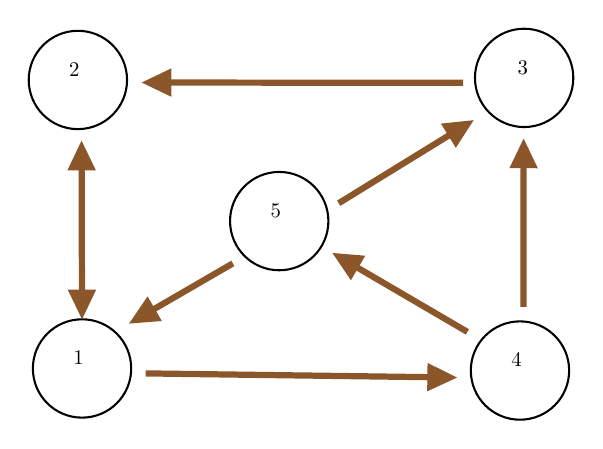
\begin{tikzpicture}[x=0.75pt,y=0.75pt,yscale=-1,xscale=1]
%uncomment if require: \path (0,300); %set diagram left start at 0, and has height of 300

%Shape: Circle [id:dp5532284801725602] 
\draw   (213.62,88.69) .. controls (213.62,75.61) and (224.22,65) .. (237.31,65) .. controls (250.39,65) and (261,75.61) .. (261,88.69) .. controls (261,101.78) and (250.39,112.38) .. (237.31,112.38) .. controls (224.22,112.38) and (213.62,101.78) .. (213.62,88.69) -- cycle ;
%Shape: Circle [id:dp7238339296497196] 
\draw   (428.62,87.69) .. controls (428.62,74.61) and (439.22,64) .. (452.31,64) .. controls (465.39,64) and (476,74.61) .. (476,87.69) .. controls (476,100.78) and (465.39,111.38) .. (452.31,111.38) .. controls (439.22,111.38) and (428.62,100.78) .. (428.62,87.69) -- cycle ;
%Shape: Circle [id:dp9299746230640014] 
\draw   (310.62,156.69) .. controls (310.62,143.61) and (321.22,133) .. (334.31,133) .. controls (347.39,133) and (358,143.61) .. (358,156.69) .. controls (358,169.78) and (347.39,180.38) .. (334.31,180.38) .. controls (321.22,180.38) and (310.62,169.78) .. (310.62,156.69) -- cycle ;
%Shape: Circle [id:dp06003655838365507] 
\draw   (215.62,227.69) .. controls (215.62,214.61) and (226.22,204) .. (239.31,204) .. controls (252.39,204) and (263,214.61) .. (263,227.69) .. controls (263,240.78) and (252.39,251.38) .. (239.31,251.38) .. controls (226.22,251.38) and (215.62,240.78) .. (215.62,227.69) -- cycle ;
%Shape: Circle [id:dp9333980197615774] 
\draw   (426.62,228.69) .. controls (426.62,215.61) and (437.22,205) .. (450.31,205) .. controls (463.39,205) and (474,215.61) .. (474,228.69) .. controls (474,241.78) and (463.39,252.38) .. (450.31,252.38) .. controls (437.22,252.38) and (426.62,241.78) .. (426.62,228.69) -- cycle ;
%Straight Lines [id:da14351861661944953] 
\draw [color={rgb, 255:red, 139; green, 87; blue, 42 }  ,draw opacity=1 ][line width=2.25]    (239.29,199) -- (239.09,122.93) ;
\draw [shift={(239.07,117.93)}, rotate = 89.84] [fill={rgb, 255:red, 139; green, 87; blue, 42 }  ,fill opacity=1 ][line width=0.08]  [draw opacity=0] (14.29,-6.86) -- (0,0) -- (14.29,6.86) -- cycle    ;
\draw [shift={(239.31,204)}, rotate = 269.84] [fill={rgb, 255:red, 139; green, 87; blue, 42 }  ,fill opacity=1 ][line width=0.08]  [draw opacity=0] (14.29,-6.86) -- (0,0) -- (14.29,6.86) -- cycle    ;
%Straight Lines [id:da17800771926651127] 
\draw [color={rgb, 255:red, 139; green, 87; blue, 42 }  ,draw opacity=1 ][line width=2.25]    (422.97,90.07) -- (273.07,89.93) ;
\draw [shift={(268.07,89.93)}, rotate = 0.05] [fill={rgb, 255:red, 139; green, 87; blue, 42 }  ,fill opacity=1 ][line width=0.08]  [draw opacity=0] (14.29,-6.86) -- (0,0) -- (14.29,6.86) -- cycle    ;
%Straight Lines [id:da8693343970271716] 
\draw [color={rgb, 255:red, 139; green, 87; blue, 42 }  ,draw opacity=1 ][line width=2.25]    (451.97,198.07) -- (452.07,121.93) ;
\draw [shift={(452.07,116.93)}, rotate = 90.07] [fill={rgb, 255:red, 139; green, 87; blue, 42 }  ,fill opacity=1 ][line width=0.08]  [draw opacity=0] (14.29,-6.86) -- (0,0) -- (14.29,6.86) -- cycle    ;
%Straight Lines [id:da6344324541430564] 
\draw [color={rgb, 255:red, 139; green, 87; blue, 42 }  ,draw opacity=1 ][line width=2.25]    (269.97,230.07) -- (414.97,232) ;
\draw [shift={(419.97,232.07)}, rotate = 180.76] [fill={rgb, 255:red, 139; green, 87; blue, 42 }  ,fill opacity=1 ][line width=0.08]  [draw opacity=0] (14.29,-6.86) -- (0,0) -- (14.29,6.86) -- cycle    ;
%Straight Lines [id:da07777304568721788] 
\draw [color={rgb, 255:red, 139; green, 87; blue, 42 }  ,draw opacity=1 ][line width=2.25]    (424.97,210.07) -- (364.28,174.59) ;
\draw [shift={(359.97,172.07)}, rotate = 30.31] [fill={rgb, 255:red, 139; green, 87; blue, 42 }  ,fill opacity=1 ][line width=0.08]  [draw opacity=0] (14.29,-6.86) -- (0,0) -- (14.29,6.86) -- cycle    ;
%Straight Lines [id:da043097960393339685] 
\draw [color={rgb, 255:red, 139; green, 87; blue, 42 }  ,draw opacity=1 ][line width=2.25]    (362.97,148.07) -- (423.71,110.69) ;
\draw [shift={(427.97,108.07)}, rotate = 148.39] [fill={rgb, 255:red, 139; green, 87; blue, 42 }  ,fill opacity=1 ][line width=0.08]  [draw opacity=0] (14.29,-6.86) -- (0,0) -- (14.29,6.86) -- cycle    ;
%Straight Lines [id:da4103672479327105] 
\draw [color={rgb, 255:red, 139; green, 87; blue, 42 }  ,draw opacity=1 ][line width=2.25]    (311.97,177.07) -- (266.29,203.56) ;
\draw [shift={(261.97,206.07)}, rotate = 329.89] [fill={rgb, 255:red, 139; green, 87; blue, 42 }  ,fill opacity=1 ][line width=0.08]  [draw opacity=0] (14.29,-6.86) -- (0,0) -- (14.29,6.86) -- cycle    ;

% Text Node
\draw (232,79.4) node [anchor=north west][inner sep=0.75pt]  [xscale=0.75,yscale=0.75]  {$2$};
% Text Node
\draw (448,78.4) node [anchor=north west][inner sep=0.75pt]  [xscale=0.75,yscale=0.75]  {$3$};
% Text Node
\draw (329,147.4) node [anchor=north west][inner sep=0.75pt]  [xscale=0.75,yscale=0.75]  {$5$};
% Text Node
\draw (234,218.4) node [anchor=north west][inner sep=0.75pt]  [xscale=0.75,yscale=0.75]  {$1$};
% Text Node
\draw (445,219.4) node [anchor=north west][inner sep=0.75pt]  [xscale=0.75,yscale=0.75]  {$4$};


\end{tikzpicture}
\end{FigureCenter}


    matrix representation
$$
A=\left[\begin{array}{lllll}
0 & 1 & 0 & 0 & 1 \\
1 & 0 & 1 & 0 & 0 \\
0 & 0 & 0 & 1 & 1 \\
1 & 0 & 0 & 0 & 0 \\
0 & 0 & 0 & 1 & 0
\end{array}\right]
$$
$ A_{i j}=1 $ indicates an edge $ j \rightarrow i $

    give a graph interpretation of $ A^{2}=A A, A^{3}=A A A, \ldots $
$$
A^{2}=\left[\begin{array}{lllll}
1 & 0 & 1 & 1 & 0 \\
0 & 1 & 0 & 1 & 2 \\
1 & 0 & 0 & 1 & 0 \\
0 & 1 & 0 & 0 & 1 \\
1 & 0 & 0 & 0 & 0
\end{array}\right], \quad A^{3}=\left[\begin{array}{lllll}
1 & 1 & 0 & 1 & 2 \\
2 & 0 & 1 & 2 & 0 \\
1 & 1 & 0 & 0 & 1 \\
1 & 0 & 1 & 1 & 0 \\
0 & 1 & 0 & 0 & 1
\end{array}\right]
$$
\end{example}


\subsection{网络中的矩阵}

In many applications a graph is used to represent a network, through which some commodity or quantity such as electricity, water, heat, or vehicular traffic flows. The edges of the graph represent the paths or links over which the quantity can move or flow, in either direction. If $ x $ is an $ m $-vector representing a flow in the network, we interpret $ x_{j} $ as the flow (rate) along the edge $ j $, with a positive value meaning the flow is in the direction of edge $ j $, and negative meaning the flow is in the opposite direction of edge $ j $. In a network, the direction of the edge or link does not specify the direction of flow; it only specifies which direction of flow we consider to be positive.

\subsubsection{Flow conservation}

When $ x $ represents a flow in a network, the matrix-vector product $ y=A x $ can be given a very simple interpretation. 

The $ n $-vector $ y=A x $ can be interpreted as the vector of net flows, from the edges, into the nodes: $ y_{i} $ is equal to the total of the flows that come in to node $ i $, minus the total of the flows that go out from node $ i $. The quantity $ y_{i} $ is sometimes called the \term{flow surplus} at node $ i $.

If $ A x=0 $, we say that \term{flow conservation} occurs, since at each node, the total inflow matches the total out-flow. In this case the flow vector $ x $ is called a \term{circulation}. This could be used as a model of traffic flow (in a closed system), with the nodes representing intersections and the edges representing road segments (one for each
direction).

\subsubsection{Sources and Sinks}

In many applications it is useful to include additional flows called \term{source flows} or \term{exogenous flows}, that enter or leave the network at the nodes, but not along the edges. We denote these flows with an $ n $-vector $ s $. 

We can think of $ s_{i} $ as a flow that enters the network at node $ i $ from outside, i.e., not from any edge. When $ s_{i}>0 $ the exogenous flow is called a \term{source}, since it is injecting the quantity into the network at the node. When $ s_{i}<0 $ the exogenous flow is called a \term{sink}, since it is removing the quantity from the network at the node.

\subsubsection{Flow Conservation with Sources}

The equation $Ax + s = 0$ means that the flow
is conserved at each node, counting the source flow: The total of all incoming flow,
from the incoming edges and exogenous source, minus the total outgoing flow from
outgoing edges and exogenous sinks, is zero.

\subsubsection{Node Potentials}

A graph is also useful when we focus on the values of some quantity at each graph vertex or node. Let $ v $ be an $ n $-vector, often interpreted as a potential, with $ v_{i} $ the potential value at node $ i $. We can give a simple interpretation to the matrix-vector product $ u=A^{T} v $. The $ m $-vector $ u=A^{T} v $ gives the potential differences across the edges: $ u_{j}=v_{l}-v_{k} $, where edge $ j $ goes from node $ k $ to node $ l $.

\subsubsection{Dirichlet Energy}

When the $ m $-vector $ A^{T} v $ is small, it means that the potential differences across the edges are small. Another way to say this is that the potentials of connected vertices are near each other. A quantitative measure of this is the function of $ v $ given by
$$
\mathcal{D}(v)=\left\|A^{T} v\right\|^{2}
$$
This function arises in many applications, and is called the Dirichlet energy (or Laplacian quadratic form) associated with the graph. It can be expressed as
$$
\mathcal{D}(v)=\sum_{\text {edges }(k, l)}\left(v_{l}-v_{k}\right)^{2}
$$

which is the sum of the squares of the potential differences of v across all edges in
the graph. The Dirichlet energy is small when the potential differences across the
edges of the graph are small, i.e., nodes that are connected by edges have similar
potential values.
The Dirichlet energy is used as a measure the non-smoothness (roughness) of
a set of node potentials on a graph. A set of node potentials with small Dirichlet
energy can be thought of as smoothly varying across the graph. Conversely, a set
of potentials with large Dirichlet energy can be thought of as non-smooth or rough.
The Dirichlet energy will arise as a measure of roughness in several applications.

\subsection{Convolution}


\begin{definition}[一维卷积]
    向量 $ a \in \mathbb{R}^{n} $ 和向量 $ b \in \mathbb{R}^{m} $ 的\term{卷积}是一个 $ ({n}+{m}-1) $ 维向量 $ c \in \mathbb{R}^{m+{n}-1} $

    $$ c_{k}=\sum_{i+j=k+1} a_{i} b_{j}, \quad k=1, \ldots n+m-1 $$

    记为 $ c=a * b$
\end{definition}

\begin{example}
    设$n=4,  m=3 $

\begin{FigureCenter}{An example of convolution}
    \tikzset{every picture/.style={line width=0.75pt}} %set default line width to 0.75pt        

    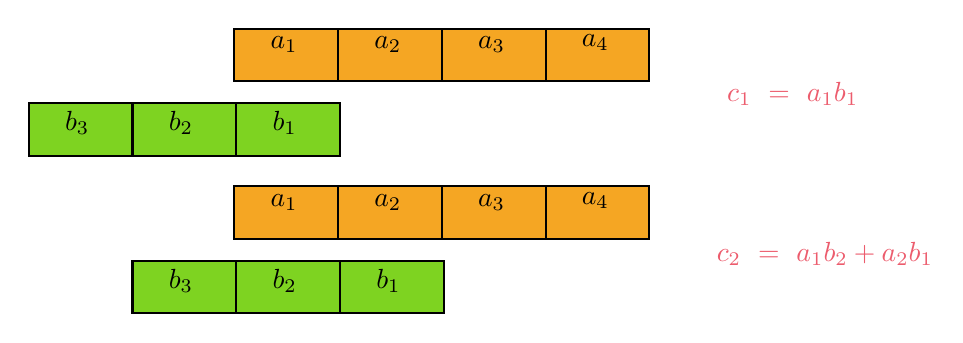
\begin{tikzpicture}[x=0.75pt,y=0.75pt,yscale=-1,xscale=1]
    %uncomment if require: \path (0,300); %set diagram left start at 0, and has height of 300
    
    %Shape: Rectangle [id:dp6383640467867335] 
    \draw  [fill={rgb, 255:red, 245; green, 166; blue, 35 }  ,fill opacity=1 ] (110,54) -- (160.01,54) -- (160.01,79.16) -- (110,79.16) -- cycle ;
    
    %Shape: Rectangle [id:dp9915913508162717] 
    \draw  [fill={rgb, 255:red, 245; green, 166; blue, 35 }  ,fill opacity=1 ] (260.01,54) -- (310.02,54) -- (310.02,79.16) -- (260.01,79.16) -- cycle ;
    %Shape: Rectangle [id:dp7574544776550791] 
    \draw  [fill={rgb, 255:red, 245; green, 166; blue, 35 }  ,fill opacity=1 ] (210,54) -- (260.01,54) -- (260.01,79.16) -- (210,79.16) -- cycle ;
    %Shape: Rectangle [id:dp15668905720803483] 
    \draw  [fill={rgb, 255:red, 245; green, 166; blue, 35 }  ,fill opacity=1 ] (160,54) -- (210.01,54) -- (210.01,79.16) -- (160,79.16) -- cycle ;
    
    %Shape: Rectangle [id:dp517800094810728] 
    \draw  [fill={rgb, 255:red, 126; green, 211; blue, 33 }  ,fill opacity=1 ] (11,90) -- (61.01,90) -- (61.01,115.16) -- (11,115.16) -- cycle ;
    %Shape: Rectangle [id:dp15583903887589012] 
    \draw  [fill={rgb, 255:red, 126; green, 211; blue, 33 }  ,fill opacity=1 ] (61,90) -- (111.01,90) -- (111.01,115.16) -- (61,115.16) -- cycle ;
    %Shape: Rectangle [id:dp4794201673076599] 
    \draw  [fill={rgb, 255:red, 126; green, 211; blue, 33 }  ,fill opacity=1 ] (111,90) -- (161.01,90) -- (161.01,115.16) -- (111,115.16) -- cycle ;
    
    %Shape: Rectangle [id:dp9652913856506695] 
    \draw  [fill={rgb, 255:red, 245; green, 166; blue, 35 }  ,fill opacity=1 ] (110,130) -- (160.01,130) -- (160.01,155.16) -- (110,155.16) -- cycle ;
    
    %Shape: Rectangle [id:dp6681556567962323] 
    \draw  [fill={rgb, 255:red, 245; green, 166; blue, 35 }  ,fill opacity=1 ] (260.01,130) -- (310.02,130) -- (310.02,155.16) -- (260.01,155.16) -- cycle ;
    %Shape: Rectangle [id:dp0819288495364412] 
    \draw  [fill={rgb, 255:red, 245; green, 166; blue, 35 }  ,fill opacity=1 ] (210,130) -- (260.01,130) -- (260.01,155.16) -- (210,155.16) -- cycle ;
    %Shape: Rectangle [id:dp015621153657017217] 
    \draw  [fill={rgb, 255:red, 245; green, 166; blue, 35 }  ,fill opacity=1 ] (160,130) -- (210.01,130) -- (210.01,155.16) -- (160,155.16) -- cycle ;
    
    %Shape: Rectangle [id:dp9772799588063847] 
    \draw  [fill={rgb, 255:red, 126; green, 211; blue, 33 }  ,fill opacity=1 ] (61,166) -- (111.01,166) -- (111.01,191.16) -- (61,191.16) -- cycle ;
    %Shape: Rectangle [id:dp8281584537494973] 
    \draw  [fill={rgb, 255:red, 126; green, 211; blue, 33 }  ,fill opacity=1 ] (111,166) -- (161.01,166) -- (161.01,191.16) -- (111,191.16) -- cycle ;
    %Shape: Rectangle [id:dp20253755057026024] 
    \draw  [fill={rgb, 255:red, 126; green, 211; blue, 33 }  ,fill opacity=1 ] (161,166) -- (211.01,166) -- (211.01,191.16) -- (161,191.16) -- cycle ;
    
    
    % Text Node
    \draw (126,56.4) node [anchor=north west][inner sep=0.75pt]    {$a_{1}$};
    % Text Node
    \draw (176,56.4) node [anchor=north west][inner sep=0.75pt]    {$a_{2}$};
    % Text Node
    \draw (226,56.4) node [anchor=north west][inner sep=0.75pt]    {$a_{3}$};
    % Text Node
    \draw (276,55.4) node [anchor=north west][inner sep=0.75pt]    {$a_{4}$};
    % Text Node
    \draw (127,92.4) node [anchor=north west][inner sep=0.75pt]    {$b_{1}$};
    % Text Node
    \draw (77,92.4) node [anchor=north west][inner sep=0.75pt]    {$b_{2}$};
    % Text Node
    \draw (27,92.4) node [anchor=north west][inner sep=0.75pt]    {$b_{3}$};
    % Text Node
    \draw (77,168.4) node [anchor=north west][inner sep=0.75pt]    {$b_{3}$};
    % Text Node
    \draw (127,168.4) node [anchor=north west][inner sep=0.75pt]    {$b_{2}$};
    % Text Node
    \draw (177,168.4) node [anchor=north west][inner sep=0.75pt]    {$b_{1}$};
    % Text Node
    \draw (276,131.4) node [anchor=north west][inner sep=0.75pt]    {$a_{4}$};
    % Text Node
    \draw (226,132.4) node [anchor=north west][inner sep=0.75pt]    {$a_{3}$};
    % Text Node
    \draw (176,132.4) node [anchor=north west][inner sep=0.75pt]    {$a_{2}$};
    % Text Node
    \draw (126,132.4) node [anchor=north west][inner sep=0.75pt]    {$a_{1}$};
    % Text Node
    \draw (346,78.4) node [anchor=north west][inner sep=0.75pt]  [color={rgb, 255:red, 236; green, 92; blue, 109 }  ,opacity=1 ]  {$c_{1} \ =\ a_{1} b_{1}$};
    % Text Node
    \draw (341,155.4) node [anchor=north west][inner sep=0.75pt]  [color={rgb, 255:red, 236; green, 92; blue, 109 }  ,opacity=1 ]  {$c_{2} \ =\ a_{1} b_{2} +a_{2} b_{1}$};
    
    
    \end{tikzpicture}
\end{FigureCenter}

    
    
$$\begin{aligned}
    c_{1}&=a_{1} b_{1}\\
    c_{2}&=a_{1} b_{2}+a_{2} b_{1}\\
    c_{3}&=a_{1} b_{3}+a_{2} b_{2}+a_{3} b_{1}\\
    c_{4}&=a_{2} b_{3}+a_{3} b_{2}+a_{4} b_{1}\\
    c_{5}&=a_{3} b_{3}+a_{4} b_{2}\\
    c_{6}&=a_{4} b_{3}\\
\end{aligned} $$


\end{example}

\begin{corollary}
    假设向量$a$和$b$分别是以下多项式的系数
    $$ p(x)=a_{1}+a_{2} x+\cdots+a_{n} x^{n-1}, q(x)=b_{1}+b_{2} x+\cdots+b_{m} x^{m-1} $$

    则 $ {c}={a}{*} {~b} $ 是多项式 $ p(x) q(x) $ 的系数.

    $$ p(x) q(x)=c_{1}+c_{2} x+\cdots+c_{m+n-1} x^{m+n-2} $$
\end{corollary}

\begin{corollary}[卷积性质]
    有如下性质:
    \begin{itemize}
        \item 对称性: $ a * b=b * a $
        \item 结合律: $ (a * b) * c=a *(b * c) $
        \item 如果 $ a * b=0 $, 则 $ a=0 $, 或者 $ b=0 $
    \end{itemize}
\end{corollary}

\begin{corollary}
    如果固定 $ a $或$b$,则 $ c=a * b $ 是一个线性函数
\end{corollary}

\begin{example}[Toeplitz Matrix]
    4维向量a和3维向量 $ b $ ,  则 $ c=a * b $

$$
\left[\begin{array}{l}
c_{1} \\
c_{2} \\
c_{3} \\
c_{4} \\
c_{5} \\
c_{6}
\end{array}\right]=\left[\begin{array}{lll}
a_{1} & 0 & 0 \\
a_{2} & a_{1} & 0 \\
a_{3} & a_{2} & a_{1} \\
a_{4} & a_{3} & a_{2} \\
0 & a_{4} & a_{3} \\
0 & 0 & a_{4}
\end{array}\right]\left[\begin{array}{l}
b_{1} \\
b_{2} \\
b_{3}
\end{array}\right]=\left[\begin{array}{cccc}
b_{1} & 0 & 0 & 0 \\
b_{2} & b_{1} & 0 & 0 \\
b_{3} & b_{2} & b_{1} & 0 \\
0 & b_{3} & b_{2} & b_{1} \\
0 & 0 & b_{3} & b_{2} \\
0 & 0 & 0 & b_{3}
\end{array}\right]\left[\begin{array}{l}
a_{1} \\
a_{2} \\
a_{3} \\
a_{4}
\end{array}\right]
$$
\end{example}

Convolution has a natural extension to multiple dimensions.

\begin{definition}[2-D convolution]
     Suppose that $ A $ is an $ m \times n $ matrix and $ B $ is a $ p \times q $ matrix. Their convolution is the $ (m+p-1) \times(n+q-1) $ matrix
$$
C_{r s}=\sum_{i+k=r+1, j+l=s+1} A_{i j} B_{k l}, \quad r=1, \ldots, m+p-1, \quad s=1, \ldots, n+q-1,
$$

where the indices are restricted to their ranges (or alternatively, we assume that $ A_{i j} $ and $ B_{k l} $ are zero, when the indices are out of range). 
\end{definition}

This is not denoted $ C=A * B $, however, in standard mathematical notation. So we will use the notation $ C=A \star B $.

The same properties that we observed for 1-D convolution hold for 2-D convolution: We have $ A \star B=B \star A,(A \star B) \star C=A \star(B \star C) $, and for fixed $ B, A \star B $ is a linear function of $ A $.

\begin{example}[moving average of a time series]
    $ n $-vector $ x $ represents a time series. The \term{3-period moving average of the time series} is the time series
$$
y_{k}=\frac{1}{3}\left(x_{k}+x_{k-1}+x_{k-2}\right), \quad k=1,2, \ldots, n+2
$$

(with $ x_{k} $ interpreted as zero for $ k<1 $ and $ k>n $ )

This can be expressed as a convolution $ y=a * x $ with $ a=(1 / 3,1 / 3,1 / 3) $.
\end{example}

\subsection{多项式}

\begin{definition}[多项式]
    \term{多项式} $ p(t) $, \term{度}为 $ n-1 $, \term{系数}为 $ x_{1}, x_{2}, \ldots, x_{n} $

    $$
p(t)=x_{1}+x_{2} t+x_{3} t^{2}+\cdots+x_{n} t^{n-1}
$$
\end{definition}

\begin{definition}[Vandermonde Matrices]
    $ {p}({t}) $ 在m个点中 $ t_{1}, t_{2}, \ldots, t_{m} $ 的值为
    $$
    \left[\begin{array}{c}
    p\left(t_{1}\right) \\
    p\left(t_{2}\right) \\
    \vdots \\
    p\left(t_{m}\right)
    \end{array}\right]=\left[\begin{array}{cccc}
    1 & t_{1} & \cdots & t_{1}^{n-1} \\
    1 & t_{2} & \cdots & t_{2}{ }^{n-1} \\
    \vdots & \vdots & \ddots & \vdots \\
    1 & t_{m} & \cdots & t_{m}{ }^{n-1}
    \end{array}\right]\left[\begin{array}{c}
    x_{1} \\
    x_{2} \\
    \vdots \\
    x_{n}
    \end{array}\right]=A x
    $$

    矩阵$A$被称为\term{Vandermonde矩阵}.
\end{definition}

\subsection{Fourier Transform}

\begin{definition}[Discrete Fourier Transform (DFT)]
    DFT将 $ n $ 维复向量 $ x $ 映射为 $ {n} $ 维复向量 $ y\left(\mathbb{C}^{n} \rightarrow \mathbb{C}^{n}\right) $

    $$ y_{k}=\sum_{\ell=1}^{n} x_{\ell} e^{-i \frac{2 \pi}{n}(k-1)(\ell-1)}, k=1, \cdots, n $$

    $$ \left[\begin{array}{c}y_{1} \\ y_{2} \\ y_{3} \\ \vdots \\ y_{n}\end{array}\right]=\left[\begin{array}{ccccc}1 & 1 & 1 & \cdots & 1 \\ 1 & \omega^{-1} & \omega^{-2} & \cdots & \omega^{-(n-1)} \\ 1 & \omega^{-2} & \omega^{-4} & \cdots & \omega^{-2(n-1)} \\ \vdots & \vdots & \vdots & \cdots & \vdots \\ 1 & \omega^{-(n-1)} & \omega^{-2(n-1)} & \cdots & \omega^{-(n-1)(n-1)}\end{array}\right]\left[\begin{array}{c}x_{1} \\ x_{2} \\ x_{3} \\ \vdots \\ x_{n}\end{array}\right] $$

   其中 $ \omega=e^{2 \pi i / n} $.
\end{definition}

DFT矩阵W的第 $ k $ 行第 $ l $ 列的元素为 $ W_{k l}=\omega^{-(k-1)(l-1)} $.

\begin{definition}[Discrete Inverse Fourier Transform]
    $$ x_{\ell}=\frac{1}{n} \sum_{k=1}^{n} y_{k} e^{i \frac{2 \pi}{n}(k-1)(\ell-1)}, \ell=1, \cdots, n $$
\end{definition}

\section{Semi-Definite Matrices}

\begin{definition}[半正定矩阵]
    对称矩阵 $ A \in \mathbb{R}^{n \times n} $ 称为\term{半正定矩阵}, 满足以下条件

$$
x^{T} A x \geq 0 \quad \forall x \in \mathbb{R}^{n}
$$
\end{definition}

\begin{definition}[正定矩阵]
    对称矩阵 $ A \in \mathbb{R}^{n \times n} $ 称为\term{正定矩阵}, 满足以下条件
$$
x^{T} A x>0 \quad \forall x \neq 0
$$
\end{definition}

\begin{definition}[二次型]
    如果$ A \in \mathbb{R}^{n \times n} $是对称矩阵, 则 $ x^{T} A x $ 是\term{二次型}函数。
\end{definition}

\begin{proof}
    $$ x^{T} A x=\sum_{i=1}^{n} \sum_{j=1}^{n} x_{i} A_{i j} x_{j}=\sum_{i=1}^{n} A_{i i} x_{i}^{2}+2 \sum_{i>j} A_{i j} x_{i} x_{j} $$
\end{proof}

\begin{example}
    $$ A=\left[\begin{array}{ll}9 & 6 \\ 6 & a\end{array}\right] $$

    $$ x^{T} A x=9 x_{1}^{2}+12 x_{1} x_{2}+a x_{2}^{2}=\left(3 x_{1}+2 x_{2}\right)^{2}+(a-4) x_{2}^{2} $$

    如果 $ a>4 $, 矩阵 $ A $ 为正定矩阵:
$$
x^{T} A x>0 \quad \forall x \neq 0
$$

如果 $ a=4 $, 矩阵 $ A $ 为半正定矩阵, 但不是正定矩阵:
$$
x^{T} A x \geq 0 \quad \forall x, \quad x^{T} A x=0 \quad \exists x=\left[\begin{array}{l}
2 \\
-3
\end{array}\right]
$$

如果 $ a<4 $, 矩阵 $ A $ 不是半正定矩阵:
$$
x^{T} A x<0 \quad \exists x=\left[\begin{array}{l}
2 \\
-3
\end{array}\right]
$$
\end{example}

\begin{theorem}
    正定矩阵 $ A $ 都是非奇异的.
\end{theorem}

\begin{proof}
    $$ A x=0 \quad \Rightarrow \quad x^{T} A x=0 \quad \Rightarrow \quad x=0 $$

    最后一步由正定性得到的.($
    x^{T} A x>0 \quad \forall x \neq 0
    $)

\end{proof}

\begin{theorem}[正定矩阵对角元素性质]
    正定矩阵 $ A $ 有正的对角元素.

    $$
A_{i i}=e_{i}^{T} A e_{i}>0
$$
\end{theorem}

\begin{theorem}[半正定矩阵对角元素性质]
    每个半正定矩阵 $ A $ 都有非负的对角元素.
$$
A_{i i}=e_{i}^{T} A e_{i} \geq 0
$$
\end{theorem}


\section{Gram 矩阵}

\begin{definition}[实矩阵$A$的Gram矩阵]
    \label{Def:Gram}

    $$ G=A^{T} A=\left[\begin{array}{c}a_{1}^{T} \\ a_{2}^{T} \\ \vdots \\ a_{n}^{T}\end{array}\right]\left[a_{1}, a_{2}, \cdots, a_{n}\right]=\left[\begin{array}{cccc}a_{1}^{T} a_{1} & a_{1}^{T} a_{2} & \cdots & a_{1}^{T} a_{n} \\ a_{2}^{T} a_{1} & a_{2}^{T} a_{2} & \cdots & a_{2}^{T} a_{n} \\ \vdots & \vdots & \ddots & \vdots \\ a_{n}^{T} a_{1} & a_{n}^{T} a_{2} & \cdots & a_{n}^{T} a_{n}\end{array}\right] $$
\end{definition}

\begin{definition}[复矩阵的$A$的Gram 矩阵]
    $$ G=A^{H} A=\left[\begin{array}{cccc}a_{1}^{H} a_{1} & a_{1}^{H} a_{2} & \cdots & a_{1}^{H} a_{n} \\ a_{2}^{H} a_{1} & a_{2}^{H} a_{2} & \cdots & a_{2}^{H} a_{n} \\ \vdots & \vdots & \ddots & \vdots \\ a_{n}^{H} a_{1} & a_{n}^{H} a_{2} & \cdots & a_{n}^{H} a_{n}\end{array}\right] $$
\end{definition}

\begin{theorem}
    每个Gram矩阵都是半正定的.
\end{theorem}

\begin{proof}
    $$ x^{T} A x=x^{T} B^{T} B x=\|B x\|_{2}^{2} \geq 0 , \forall x $$
\end{proof}

\begin{theorem}
    如果Gram矩阵是正定的, 则要满足
    $$ x^{T} A x=x^{T} B^{T} B x=\|B x\|_{2}^{2}>0 ( \forall x \neq 0) $$
\end{theorem}

\begin{corollary}
    如果Gram矩阵是正定的, 则$B$的列向量是线性无关的.
\end{corollary}

\begin{proof}
    $$\|B x\|_{2}^{2}>0 ( \forall x \neq 0)$$

所以 $\forall x \neq 0, Bx \neq 0  $.

    注意和线性无关 \ref{Def:LinearIndependence} 的定义进行参照.
\end{proof}

\section{Affine functions and matrix-vector product}


回想仿射函数、泰勒展开的定义。

For fixed $ A \in \mathbf{R}^{m \times n}, b \in \mathbf{R}^{m} $, define a function $ f: \mathbf{R}^{n} \rightarrow \mathbf{R}^{m} $ by
$$
f(x)=A x+b
$$
i.e., a matrix-vector product plus a constant.

Any function of this type is affine: if $ \alpha+\beta=1 $ then
$$
A(\alpha x+\beta y)+b=\alpha(A x+b)+\beta(A y+b)
$$

Every affine function can be written as $ f(x)=A x+b $ with:
$$
A=\left[\begin{array}{llll}
f\left(e_{1}\right)-f(0) & f\left(e_{2}\right)-f(0) & \cdots & f\left(e_{n}\right)-f(0)
\end{array}\right]
$$
and $ b=f(0) $.

\begin{theorem}
    First-order Taylor approximation of differentiable $ f: \mathbf{R}^{n} \rightarrow \mathbf{R}^{m} $ around $ z $

$$
\hat{f_{i}}(x)=f_{i}(z)+\frac{\partial f_{i}}{\partial x_{1}}(z)\left(x_{1}-z_{1}\right)+\cdots+\frac{\partial f_{i}}{\partial x_{n}}(z)\left(x_{n}-z_{n}\right), \quad i=1, \ldots, m
$$

in matrix-vector notation: $ \hat{f}(x)=f(z)+D f(z)(x-z) $ where
$$
D f(z)=\left[\begin{array}{cccc}
\frac{\partial f_{1}}{\partial x_{1}}(z) & \frac{\partial f_{1}}{\partial x_{2}}(z) & \cdots & \frac{\partial f_{1}}{\partial x_{n}}(z) \\
\frac{\partial f_{2}}{\partial x_{1}}(z) & \frac{\partial f_{2}}{\partial x_{2}}(z) & \cdots & \frac{\partial f_{2}}{\partial x_{n}}(z) \\
\vdots & \vdots & & \vdots \\
\frac{\partial f_{m}}{\partial x_{1}}(z) & \frac{\partial f_{m}}{\partial x_{2}}(z) & \cdots & \frac{\partial f_{m}}{\partial x_{n}}(z)
\end{array}\right]=\left[\begin{array}{c}
\nabla f_{1}(z)^{T} \\
\nabla f_{2}(z)^{T} \\
\vdots \\
\nabla f_{m}(z)^{T}
\end{array}\right]
$$

$ D f(z) $ is called the \term{derivative matrix} or \term{Jacobian matrix} of $ f $ at $ z $, $ \hat{f} $ is a local affine approximation of $ f $ around $ z $.
\end{theorem}


\chapter{Matrices Norms}

\section{矩阵范数}

\begin{definition}[Matrix Norm]
    向量空间中存在一个函数 $ \|\cdot\|: \mathbb{R}^{m \times n} \rightarrow \mathbb{R} $

    且满足以下条件:

    \begin{itemize}
        \item 齐次性: $ \|\alpha A\|=|\alpha|\|A\|, \alpha \in \mathbb{R} $ 且 $ A \in \mathbb{R}^{m \times n} $;
        \item 三角不等式: $ \|A+B\| \leq\|A\|+\|B\|, A, B \in \mathbb{R}^{m \times n} $;
        \item 非负性: $ \|A\| \geq 0, A \in \mathbb{R}^{m \times n} $ 且 $ \|A\|=0 \Leftrightarrow A=0 $;
    \end{itemize}

则称 $ \|\cdot\| $ 为矩阵范数. 
\end{definition}

向量空间 $ \mathbb{R}^{m \times n} $ 矩阵范数:

\begin{example}[F-范数(Frobenius norm)]
    $$ \|A\|_{F}=\left(\sum_{i=1}^{n} \sum_{j=1}^{n} a_{i j}^{2}\right)^{\frac{1}{2}} $$
\end{example}

\begin{proof}
    $$ \|A\|_{F} \geq 0 $$

    $$ \|\alpha A\|_{F}=|\alpha|\|A\|_{F}, \alpha \in \mathbb{R} $$

    $$ \begin{aligned}\|A+B\|_{F}=&\left(\sum_{i=1}^{n} \sum_{j=1}^{n}\left(a_{i j}+b_{i j}\right)^{2}\right)^{\frac{1}{2}} \leq\left(\sum_{i=1}^{n} \sum_{j=1}^{n}\left(a_{i j}\right)^{2}\right)^{\frac{1}{2}}+\left(\sum_{i=1}^{n} \sum_{j=1}^{n}\left(b_{i j}\right)^{2}\right)^{\frac{1}{2}} \\ &=\|A\|_{F}+\|B\|_{F} \end{aligned} $$
\end{proof}

\begin{definition}[从属于给定向量范数 $ \|x\|_{v} $ 的矩阵范数]
    设 $ x \in \mathbb{R}^{n}, A \in \mathbb{R}^{m \times n},\|\cdot\|_{v} $ 为一种向量范数. 则 $ \frac{\|A x\|_{v}}{\|x\|_{v}} $ 对所有 $ x \neq 0 $ 有最大值, 令

    $$ \|A\|_{v}=\max _{x \neq 0}\left\{\frac{\|A x\|_{v}}{\|x\|_{v}}\right\}=\max _{x \neq 0}\left\{\left\|A \frac{x}{\|x\|_{v}}\right\|_{v}\right\}=\max _{\|y\|_{v}=1}\left\{\|A y\|_{v}\right\} $$

    即$$ \|A\|_{v}=\max _{x \neq 0}\left\{\frac{\|A x\|_{v}}{\|x\|_{v}}\right\} $$

    $ \|A\|_{v} $ 称为从属于给定向量范数 $ \|x\|_{v} $ 的矩阵范数, 简称为\term{从属范数}或\term{算子范数}.
\end{definition}

\begin{proof}
    可以验证 $ \|A\|_{v} $ 满足矩阵范数定义. 

    $$ \|A\|_{v} \geq 0 $$

    $$ \|\alpha A\|_{v}=|\alpha|\|A\|_{v}, \alpha \in \mathbb{R} $$

    $$\begin{aligned}
        \|A+B\|_{v} &=\max _{\|y\|_{v}=1}\|(A+B) y\|_{v} \\
        &\leq \max _{\|y\|_{v}=1}\left\{\|A y\|_{v}+\|B y\|_{v}\right\} \\
        & \leq \max _{\|y\|_{v}=1}\|A y\|_{v}+\max _{\|y\|_{v}=1}\|B y\|_{v} \\
        & =\|A\|_{v}+\|B\|_{v}
    \end{aligned}$$

\end{proof}

\begin{remark}
    在本书中若未明确说明, $\|A \|$表示的是算子范数.
\end{remark}

由定义 $ \|A\|_{v}=\max _{x \neq 0}\left\{\frac{\|A x\|_{v}}{\|x\|_{v}}\right\} $ 可得

\begin{definition}[向量范数和算子范数相容]
    $$ \frac{\|A x\|_{v}}{\|x\|_{v}} \leq\|A\|_{v} \Rightarrow\|A x\|_{v} \leq\|A\|_{v}\|x\|_{v} $$

    称向量范数和算子范数\term{相容}. 
\end{definition}

\begin{theorem}[算子范数服从乘法范数相容性]
   对于 $ A \in \mathbb{R}^{m \times n}, B \in \mathbb{R}^{n \times p} $

    $$\begin{aligned}
        \|A B\|_{v} &=\max _{x \neq 0}\left\{\frac{\|A B x\|_{v}}{\|x\|_{v}}\right\} \\
        & \leq \max _{x \neq 0}\left\{\frac{\|A\|_{v}\|B x\|_{v}}{\|x\|_{v}}\right\} \\
        & \leq\|A\|_{v} \max _{x \neq 0}\left\{\frac{\|B\|_{v}\|x\|_{v}}{\|x\|_{v}}\right\} \\
        & =\|A\|_{v}\|B\|_{v}
    \end{aligned}$$
    算子范数服从\term{乘法范数相容性}.
\end{theorem}

根据向量的常用范数可以导出矩阵 $ A \in \mathbb{R}^{m \times n} $ 的算子范数

\begin{definition}[$A$的列范数]
    $$ \|A\|_{1}=\max _{x \neq 0}\left(\frac{\|A x\|_{1}}{\|x\|_{1}}\right)=\max _{1 \leq j \leq n} \sum_{i=1}^{m}\left|a_{i j}\right| $$
\end{definition}

\begin{definition}[$A$的行范数]
    $$ \|A\|_{\infty}=\max _{x \neq 0}\left( \frac{\|A x\|_{\infty}}{\|x\|_{\infty}}    \right)=\max _{1 \leq i \leq m} \sum_{j=1}^{n}\left|a_{i j}\right| $$
\end{definition}

\begin{definition}[$A$的2-范数]
    \begin{equation}
        \label{eqn:a-l2-norm}
        \|A\|_{2}=\max _{x \neq 0}\left( \frac{\|A x\|_{2}}{\|x\|_{2}}  \right)=\sqrt{\lambda_{\max }\left(A^{T} A\right)}
    \end{equation}
    $$  $$
\end{definition}

\begin{proof}
    For any $A$ Choose $x$ to be the eigenvector of $A^{{T}} A$ with largest eigenvalue $\lambda_{\max } .$ The ratio in equation \ref{eqn:a-l2-norm} is $\boldsymbol{x}^{{T}} A^{{T}} A \boldsymbol{x}=\boldsymbol{x}^{{T}}\left(\lambda_{\max }\right) \boldsymbol{x}$ divided by $\boldsymbol{x}^{{T}} \boldsymbol{x}$. This is $\lambda_{\max }$.

No $\boldsymbol{x}$ can give a larger ratio. The symmetric matrix $A^{{T}} A$ has eigenvalues $\lambda_{1}, \ldots, \lambda_{n}$ and orthonormal eigenvectors $q_{1}, \boldsymbol{q}_{2}, \ldots, \boldsymbol{q}_{n} .$ Every $\boldsymbol{x}$ is a combination of those vectors. Try this combination in the ratio and remember that $\boldsymbol{q}_{i}^{{T}} \boldsymbol{q}_{j}=0$ :
$$
\frac{\boldsymbol{x}^{{T}} A^{{T}} A \boldsymbol{x}}{\boldsymbol{x}^{{T}} \boldsymbol{x}}=\frac{\left(c_{1} \boldsymbol{q}_{1}+\cdots+c_{n} \boldsymbol{q}_{n}\right)^{{T}}\left(c_{1} \lambda_{1} \boldsymbol{q}_{1}+\cdots+c_{n} \lambda_{n} \boldsymbol{q}_{n}\right)}{\left(c_{1} \boldsymbol{q}_{1}+\cdots+c_{n} \boldsymbol{q}_{n}\right)^{{T}}\left(c_{1} \boldsymbol{q}_{1}+\cdots+c_{n} \boldsymbol{q}_{n}\right)}=\frac{c_{1}^{2} \lambda_{1}+\cdots+c_{n}^{2} \lambda_{n}}{c_{1}^{2}+\cdots+c_{n}^{2}}
$$
The maximum ratio $\lambda_{\max }$ is when all $c$ 's are zero, except the one that multiplies $\lambda_{\max }$.
\end{proof}

\begin{remark}
    The ratio in equation \ref{eqn:a-l2-norm} is the Rayleigh quotient for the symmetric matrix $A^{{T}} A$. Its maximum is the largest eigenvalue $\lambda_{\max }\left(A^{{T}} A\right) .$ The minimum ratio is $\lambda_{\min }\left(A^{{T}} A\right)$. If you substitute any vector $\boldsymbol{x}$ into the Rayleigh quotient $\boldsymbol{x}^{{T}} A^{{T}} A \boldsymbol{x} / \boldsymbol{x}^{{T}} \boldsymbol{x}$, you are guaranteed to get a number between $\lambda_{\min }\left(A^{{T}} A\right)$ and $\lambda_{\max }\left(A^{{T}} A\right)$.
\end{remark}

\begin{corollary}
    $$\|A\|_{2}= \sigma_{\max} $$
\end{corollary}

\begin{proof}
    The norm $\|A\|$ equals the largest singular value $\sigma_{\max }$ of $A$. The singular values $\sigma_{1}, \ldots, \sigma_{r}$ are the square roots of the positive eigenvalues of $A^{{T}} A$. So certainly $\sigma_{\max }=\left(\lambda_{\max }\right)^{1 / 2}$. Since $U$ and $V$ are orthogonal in $A=U \Sigma V^{{T}}$, the norm is $\|\boldsymbol{A}\|=$ $\sigma_{\max }$.
\end{proof}

\begin{example}
    求矩阵$A$的各种常用范数
$$
A=\left(\begin{array}{ccc}
1 & 2 & 0 \\
-1 & 2 & -1 \\
0 & 1 & 1
\end{array}\right)
$$

$$ \|A\|_{1}=\max _{1 \leq j \leq n} \sum_{i=1}^{n}\left|a_{i j}\right|=\max _{1 \leq j \leq n}\{2,5,2\}=5 $$

$$ \|A\|_{\infty}=\max _{1 \leq i \leq n} \sum_{j=1}^{n}\left|a_{i j}\right|=\max _{1 \leq i \leq n}\{3,4,2\}=4 $$

由于 $ \|A\|_{2}=\sqrt{\lambda_{\max }\left(A^{T} A\right)} $
, 因此先求 $ A^{T} A $ 的特征值

$$ A^{T} A=\left(\begin{array}{ccc}1 & -1 & 0 \\ 2 & 2 & 1 \\ 0 & -1 & 1\end{array}\right) \cdot\left(\begin{array}{ccc}1 & 2 & 0 \\ -1 & 2 & -1 \\ 0 & 1 & 1\end{array}\right)=\left(\begin{array}{ccc}2 & 0 & 1 \\ 0 & 9 & -1 \\ 1 & -1 & 2\end{array}\right) $$

特征方程为

$$ \operatorname{det}\left(\lambda I-A^{T} A\right)=\left|\begin{array}{ccc}\lambda-2 & 0 & -1 \\ 0 & \lambda-9 & 1 \\ -1 & 1 & \lambda-2\end{array}\right|=0 $$

可得 $ A^{T} A $ 的特征值

$$ \lambda_{1}=9.1428, \lambda_{2}=2.9211, \lambda_{3}=0.9361 $$

\end{example}

\begin{remark}
    对于$\|A\|_{2}$需要计算$\lambda_{\max }\left(A^{T} A\right)$, 直接根据特征方程计算特征值的算法复杂度太高.
\end{remark}

\chapter{适定问题}

\section{The Definition of Well-posed Problem}

In 1923, the French mathematician Hadamard introduced the notion of well-posed (适定)  problem:

\begin{itemize}
    \item A solution for the problem exists;
    \item The solution is unique;
    \item Perturbations in the data should cause small perturbations in the solution.
\end{itemize}

One of these conditions is not satisfied, the problem is said to be ill-posed (病态) and demands a special consideration.

\begin{definition}
    假设 $ A $ 是非奇异矩阵 $$ A x=b $$

    如果将 $ b $ 为 $ b+\Delta b $, 方程新的解 $ x+\Delta x $, 则有:
$$
A(x+\Delta x)=b+\Delta b
$$

即
$$
\Delta x=A^{-1} \Delta b
$$

如果小的变化 $ \Delta b $ 导致小变化 $ \Delta x $, 则称解是\term{稳定}的. 如果小的变化 $ \Delta b $ 导致大变化 $ \Delta x $, 则称解\term{不稳定}的. 
\end{definition}

\begin{example}
    设$$ A=\frac{1}{2}\left[\begin{array}{cc}1 & 1 \\ 1+10^{-10} & 1-10^{-10}\end{array}\right], \quad A^{-1}=\left[\begin{array}{cc}1-10^{10} & 10^{10} \\ 1+10^{10} & -10^{10}\end{array}\right] $$

若$ b=(1,1) $, 方程 $ A x $ 的解 $ x=(1,1) $ . 
如果将b改为 $ b+\Delta b $ , 那么 $ x $ 的变化量为

$$ \Delta x=A^{-1} \Delta b=\left[\begin{array}{l}\Delta b_{1}-10^{10}\left(\Delta b_{1}-\Delta b_{2}\right) \\ \Delta b_{1}+10^{10}\left(\Delta b_{1}-\Delta b_{2}\right)\end{array}\right] $$
\end{example}


很小变化 $ \Delta b $ 会导致非常大变化 $ \Delta x $! 由矩阵$A$定义的问题, 称为\term{适定问题}或\term{病态问题}. 



\section{绝对误差的界限}

假设 $ A $ 是非奇异的, 并给出定义:

\begin{notation}
    $$ x=A^{-1} b$$ 
    
    $$ \Delta x=A^{-1} \Delta b $$
\end{notation}

\begin{theorem}[绝对误差的界限]
    $ \|\Delta x\| $ 的上界为
    $$
    \|\Delta x\|_{2} \leq\left\|A^{-1}\right\|_{2}\|\Delta b\|_{2}
    $$

\end{theorem}

矩阵范数 $ \left\|A^{-1}\right\|_{2} $ 小时, 当 $ \|\Delta b\|_{2} $ 变化很小, $ \|\Delta x\|_{2} $ 也很小; $ \left\|A^{-1}\right\|_{2} $ 大时,  $ \|\Delta x\|_{2} $ 可能很大,  即使 $ \|\Delta b\|_{2} $ 很小. 

\section[相对误差的界限]{相对误差的界限\footnote{Reference: \href{https://blogs.mathworks.com/cleve/2017/07/17/what-is-the-condition-number-of-a-matrix/?from=cn}{MathWorks Blog}.}}

\begin{theorem}[相对误差的界限]
    相对误差的界限是
    $$ \frac{\|\Delta x\|_{2}}{\|x\|_{2}} \leq\|A\|_{2}\left\|A^{-1}\right\|_{2} \frac{\|\Delta b\|_{2}}{\|b\|_{2}} $$
\end{theorem}

假设 $ b \neq 0 $; 因此 $ x \neq 0$

$\|\Delta x\|_{2} /\|x\|_{2} $ 的上界为:

$$ 
\begin{aligned}
    &\|\Delta x\|_{2}=\left\|A^{-1} \Delta b\right\|_{2} \leq\left\|A^{-1}\right\|_{2}\|\Delta b\|_{2}(向量范数和算子范数相容)\\
    \Rightarrow& \frac{\|\Delta x\|_{2}}{\|x\|_{2}} \leq \frac{\left\|A^{-1}\right\|_{2}\|\Delta b\|_{2}}{\|x\|_{2}}=\frac{\|A\|_{2}\left\|A^{-1}\right\|_{2}\|\Delta b\|_{2}}{\|x\|_{2}\|A\|_{2}} \leq \frac{\|A\|_{2}\left\|A^{-1}\right\|_{2}\|\Delta b\|_{2}}{\|b\|_{2}}
\end{aligned}
$$

由 $ \|b\|_{2}=\|A x\|_{2} \leq\|A\|_{2}\|x\|_{2} $, 可得

$$ \frac{\|\Delta x\|_{2}}{\|x\|_{2}} \leq\|A\|_{2}\left\|A^{-1}\right\|_{2} \frac{\|\Delta b\|_{2}}{\|b\|_{2}} $$

$ \|A\|_{2}\left\|A^{-1}\right\|_{2} $ 小,当 $ \frac{\|\Delta b\|_{2}}{\|b\|_{2}}  $ 相对变化很小时, $ \frac{\|\Delta x\|_{2}}{\|x\|_{2}}  $ 也 变化很小;

$ \|A\|_{2}\left\|A^{-1}\right\|_{2} $ 大, $ \frac{\|\Delta x\|_{2}}{\|x\|_{2}}  $ 可远远大于 $ \frac{\|\Delta b\|_{2}}{\|b\|_{2}}  $.


\begin{definition}[非奇异矩阵 $ A $ 的条件数(condition number) ]        
    条件数定义

    $$ \kappa(A)=\|A\|_{2}\left\|A^{-1}\right\|_{2} $$
\end{definition}

\begin{corollary}[非奇异矩阵 $ A $ 的条件数(condition number)性质]
    有如下性质:

    \begin{itemize}
        \item 对于所有 $ A $, 有 $ \kappa(A) \geq 1 $;
        \item 如果 $ \kappa(A) $ 比较小 (接近1),  $ x $ 的相对误差接近 $ b $ 的相对误差;
        \item 如果 $ \kappa(A) $ 比较大(超过100),  $ x $ 的相对误差比 $ b $ 的相对误差大得多. 
    \end{itemize}
\end{corollary}



\section{Cancellation}

Instability in an algorithm is often (but not always) caused by an effect called cancellation. Cancellation occurs when two numbers are subtracted that are almost equal, and one of the numbers or both are subject to error (for example, due to rounding error in previous calculations).
Suppose
$$
\hat{x}=x+\Delta x, \quad \hat{y}=y+\Delta y
$$
are approximations of two numbers $ x, y $, with absolute errors $ |\Delta x| $ and $ |\Delta y| $, respectively. The relative error in the difference $ \hat{x}-\hat{y} $ is
$$
\frac{|(\hat{x}-\hat{y})-(x-y)|}{|x-y|}=\frac{|\Delta x-\Delta y|}{|x-y|} \leq \frac{|\Delta x|+|\Delta y|}{|x-y|} .
$$

(The upper bound is achieved when $ \Delta x $ and $ \Delta y $ have opposite signs.) We see that if $ x-y $ is small, then the relative error in $ \hat{x}-\hat{y} $ can be very large, and much larger than the relative errors in $ \hat{x} $ and $ \hat{y} $. The result is that the relative errors $ |\Delta x| /|x| $, $ |\Delta y| /|y| $ are magnified enormously.

For example, suppose $ x=1, y=1+10^{-5} $, and $ x $ and $ y $ have been calculated with an accuracy of about 10 significant digits, i.e., $ |\Delta x| /|x| \approx 10^{-10} $ and $ |\Delta y| /|y| \approx $ $ 10^{-10} $. The error in the result is
$$
\frac{|(\hat{x}-\hat{y})-(x-y)|}{|x-y|} \leq \frac{|\Delta x|+|\Delta y|}{|x-y|} \approx \frac{2 \cdot 10^{-10}}{|x-y|}=2 \cdot 10^{-5} .
$$
The result has only about 5 correct digits.


\begin{example}
    Example The most straightforward method for computing the two roots of the quadratic equation
$$
a x^{2}+b x+c=0
$$
(with $ a \neq 0 $ ) is to evaluate the expressions
$$
x_{1}=\frac{-b+\sqrt{b^{2}-4 a c}}{2 a}, \quad x_{2}=\frac{-b-\sqrt{b^{2}-4 a c}}{2 a} .
$$
This method is unstable if $ b^{2} \gg|4 a c| $. If $ b>0 $, there is a danger of cancellation in the expression for $ x_{1} $; if $ b<0 $, cancellation may occur in the expression for $ x_{2} $.
For example, suppose $ a=c=1, b=10^{5}+10^{-5} $. The exact roots are given by
$$
x_{1}=\frac{-b+\sqrt{b^{2}-4 a c}}{2 a}=-10^{-5}, \quad x_{2}=\frac{-b-\sqrt{b^{2}-4 a c}}{2 a}=-10^{5},
$$
We evaluate these expressions in MATLAB, rounding the square roots to 6 correct digits using the \verb|chop| function:

\begin{lstlisting}[caption=example 1 for cancellation,language=matlab]
>> a = 1; b = 1e5 + 1e-5; c = 1;
>> x1 = (-b + chop(sqrt(b^2 - 4*a*c), 6)) / (2*a)
ans =
-5.0000e-6
>> x2 = (-b - chop(sqrt(b^2 - 4*a*c), 6)) / (2*a)
ans =
-1.0000e+05
\end{lstlisting}


The relative error in $ x_{1} $ is $ 50 \% $, and is due to cancellation.
We can formulate an algorithm that is more stable if $ b^{2} \gg|4 a c| $ as follows. First suppose $ b>0 $, so we have cancellation in the expression for $ x_{1} $. In this case we can calculate $ x_{2} $ accurately. The expression for $ x_{1} $ can be reformulated as
$$
\begin{aligned}
x_{1} &=\frac{\left(-b+\sqrt{b^{2}-4 a c}\right)\left(-b-\sqrt{b^{2}-4 a c}\right)}{(2 a)\left(-b-\sqrt{b^{2}-4 a c}\right)} \\
&=\frac{b^{2}-b^{2}+4 a c}{(2 a)\left(-b-\sqrt{b^{2}-4 a c}\right)} \\
&=\frac{c}{a x_{2}}
\end{aligned}
$$

Similarly, if $ b>0 $, we can use the expression $ x_{2}=c /\left(a x_{1}\right) $ to compute $ x_{2} $, given $ x_{1} $. The modified algorithm that avoids cancellation is therefore:

\begin{itemize}
    \item if $ b \leq 0 $, calculate
$$
x_{1}=\frac{-b+\sqrt{b^{2}-4 a c}}{2 a}, \quad x_{2}=\frac{c}{a x_{1}}
$$
    \item if $ b>0 $, calculate
$$
x_{2}=\frac{-b-\sqrt{b^{2}-4 a c}}{2 a}, \quad x_{1}=\frac{c}{a x_{2}}
$$
\end{itemize}


For the example, we get

\begin{lstlisting}[caption=example 2 for cancellation,language=matlab]
>> a = 1; b = 1e5 + 1e-5; c = 1;
>> x2 = (-b - chop(sqrt(b^2 - 4*a*c), 6)) / (2*a)
ans =
-1.0000e+05
>> x1 = c / (a*x2)
ans =
-1.0000e-05
\end{lstlisting}


\end{example}





\part{Matrices Computations}
\chapter{Inverse of Matrices}

\section{Left Inverse, Right Inverse, Inverse}

\begin{definition}[$A$的左逆]
    当一个矩阵X满足 $$ X A=I $$ 
    
    X被称为 $ A $ 的\textit{左逆}; 当左逆存在时,则称A是\textit{可左逆}的;
\end{definition}

    如果左逆矩阵存在, 则左逆矩阵有\textbf{无穷多}个.

\begin{example}
    $$ A=\left[\begin{array}{cc}-3 & -4 \\ 4 & 6 \\ 1 & 1\end{array}\right] $$

    矩阵$A$是可左逆的,其左逆矩阵有两个

    $$ B=\frac{1}{9}\left[\begin{array}{ccc}-11 & -10 & 16 \\ 7 & 8 & -11\end{array}\right] \quad C=\frac{1}{2}\left[\begin{array}{ccc}0 & -1 & 6 \\ 0 & 1 & -4\end{array}\right] $$
\end{example}

\begin{definition}[$A$的右逆]
    当左逆存在时,则称A是可左逆的;
\end{definition}

    如果右逆矩阵存在, 则右逆矩阵有\textbf{无穷多}个.


\begin{example}
    $$ B=\left[\begin{array}{lll}1 & 0 & 1 \\ 0 & 1 & 1\end{array}\right] $$

    矩阵$B$可右逆,以下矩阵都是$B$的右逆

    $$ D=\frac{1}{2}\left[\begin{array}{cc}1 & -1 \\ -1 & 1 \\ 1 & 1\end{array}\right], E=\left[\begin{array}{ll}1 & 0 \\ 0 & 1 \\ 0 & 0\end{array}\right], G=\left[\begin{array}{cc}1 & -1 \\ 0 & 0 \\ 0 & 1\end{array}\right] $$
\end{example}

一个大小为 $ m \times n $ 的矩阵, 其左逆或右逆的维度为 $ n \times m $.

\begin{theorem}
    A的左逆为 $ X $ 当且仅当 $ X^{T} $ 是 $ A^{T} $ 的右逆.
\end{theorem}

\begin{proof}
    $$
A^{T} X^{T}=(X A)^{T}=I
$$
\end{proof}

\begin{theorem}
    A的右逆为 $ X $ 当且仅当 $ X^{T} $ 是 $ A^{T} $ 的左逆.
\end{theorem}

\begin{proof}
    $$
X^{T} A^{T}=(A X)^{\mathrm{T}}=I
$$
\end{proof}

\begin{theorem}
    如果矩阵A存在左逆和右逆,则左逆和右逆一定相等
\end{theorem}

\begin{proof}
    $$
    \begin{aligned}
    &X A=I, A Y=I  \\
    \Rightarrow&  X=X I=X(A Y)=(X A) Y=Y \\
    \Rightarrow& X=Y
    \end{aligned}
$$
\end{proof}

\begin{definition}
    如果矩阵A存在左逆和右逆, 此时X称为矩阵的\textit{逆},记作 $ A^{-1} $ 当矩阵的逆存在时,则称矩阵A\textit{可逆}.
\end{definition}

\section{Linear Equation Systems}

\begin{definition}
    有$n$个变量的$m$个方程为

    $$ \left\{\begin{array}{c}A_{11} x_{1}+A_{12} x_{2}+\cdots+A_{1 n} x_{n}=b_{1} \\ A_{21} x_{1}+A_{22} x_{2}+\cdots+A_{2 n} x_{n}=b_{2} \\ \vdots \\ A_{m 1} x_{1}+A_{m 2} x_{2}+\cdots+A_{m n} x_{n}=b_{m}\end{array}\right. $$

    写成矩阵形式为: $ \mathrm{A} x=\mathrm{b} $ . 其中$A$为系数矩阵, $ x $ 为$n$维列向量. 
\end{definition}

该方程组可能\textbf{无解},\textbf{有唯一解}和\textbf{无穷解}.

\subsection{线性方程组求解}

\begin{theorem}
    如果矩阵$A$可左逆,假设 $ X $ 是矩阵$A$的左逆,则\textbf{至多}一个解, 如有解则 $ x=X b $ . 
\end{theorem}

\begin{proof}
    $$
A x=b \Rightarrow  x=X A x=X b
$$

    列满秩时(下面证明), 列向量线性无关, 所以其零空间中只有零解,方程 $ {Ax}={b} $ 可能有一个唯一解 ($b$在$A$的列空间中, 此特解就是全部解, 因为通常的特解可以通过零空间中的向量扩展出一组解集,而此时零空间只有$0$向量), 也可能无解 ($b$不在$A$的列空间中). 
\end{proof}

\begin{theorem}
    如果矩阵$A$可右逆,假设 $ Y $ 是矩阵$A$的右逆,则\textbf{至少}一个解, 即 $ x=\mathrm{Y} b $ . 
\end{theorem}

\begin{proof}
    设$x=Y b$ 

    $$
x=Y b  \Rightarrow  A x=A Y b=b
$$


右逆就是研究 $m \times n $ 矩阵$A$行满秩的情况, 此时 $ \mathrm{n}>\mathrm{m}=\operatorname{rank}(\mathrm{A}) $ . 对称的, 其左零空间中仅有零向量,即没有行向量的线性组合能够得到零向量. ($N(A ^T ) = \{0\}$)
\end{proof}

\begin{theorem}
    如果矩阵$A$可逆的,假设 $ X $ 是矩阵$A$的逆,则
$$
A x=b  \Rightarrow  x=A^{-1} b
$$
唯一解. 
\end{theorem}

\section{Fundamental Theorem of Linear Algebra}

\begin{FigureCenter}{Four Subspace of Matrix $A$}
    \tikzset{every picture/.style={line width=0.75pt}} %set default line width to 0.75pt        
    % \resizebox{\textwidth}{!}{%
    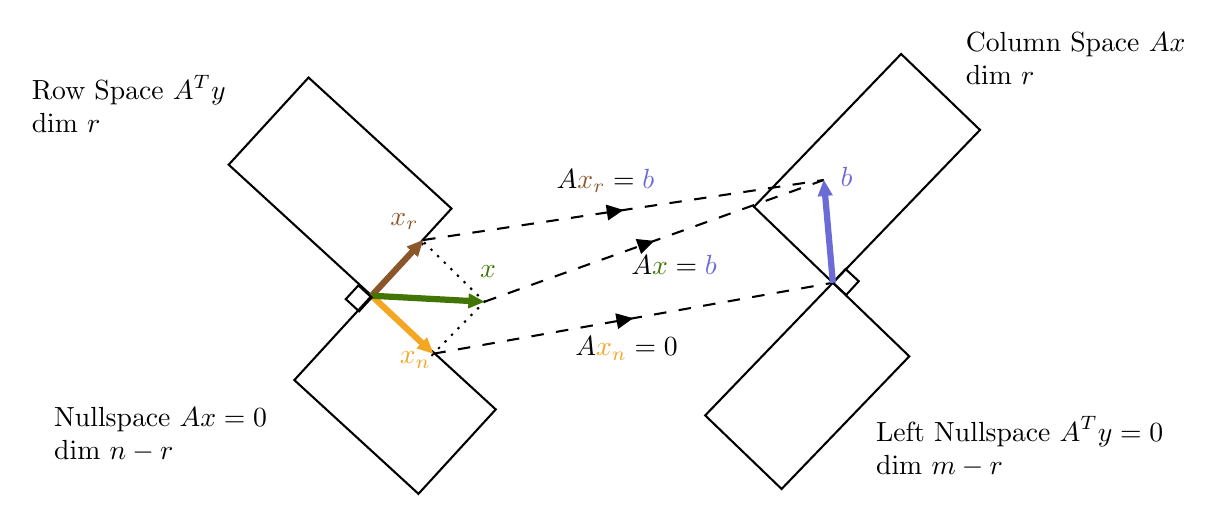
\begin{tikzpicture}[x=0.75pt,y=0.75pt,yscale=-0.9,xscale=0.9]
    
    %\begin{adjustbox}{width=\textwidth}
    %\begin{tikzpicture}   
    %uncomment if require: \path (0,300); %set diagram left start at 0, and has height of 300
    
    %Shape: Rectangle [id:dp8564537788335302] 
    \draw  [dash pattern={on 0.84pt off 2.51pt}] (221.63,153.4) -- (253.96,185.17) -- (225.93,213.7) -- (193.59,181.93) -- cycle ;
    %Shape: Rectangle [id:dp7748103688398633] 
    \draw   (159.81,65.14) -- (236.34,135.27) -- (193.59,181.93) -- (117.06,111.79) -- cycle ;
    %Shape: Rectangle [id:dp3534850306924755] 
    \draw   (193.59,181.93) -- (260.03,242.81) -- (218.64,287.99) -- (152.2,227.1) -- cycle ;
    
    %Shape: Rectangle [id:dp11468847928918202] 
    \draw   (477.03,52.53) -- (398.27,134.34) -- (440.51,175) -- (519.26,93.19) -- cycle ;
    %Shape: Rectangle [id:dp8320016424104848] 
    \draw   (440.51,175) -- (372.14,246.02) -- (413.05,285.39) -- (481.41,214.38) -- cycle ;
    
    %Straight Lines [id:da413550032058265] 
    \draw [color={rgb, 255:red, 139; green, 87; blue, 42 }  ,draw opacity=1 ][line width=2.25]    (193.59,181.93) -- (217.74,155.81) ;
    \draw [shift={(221.14,152.14)}, rotate = 492.75] [fill={rgb, 255:red, 139; green, 87; blue, 42 }  ,fill opacity=1 ][line width=0.08]  [draw opacity=0] (8.57,-4.12) -- (0,0) -- (8.57,4.12) -- cycle    ;
    %Straight Lines [id:da05215716031511208] 
    \draw [color={rgb, 255:red, 245; green, 166; blue, 35 }  ,draw opacity=1 ][line width=2.25]    (193.59,181.93) -- (222.99,209.56) ;
    \draw [shift={(226.64,212.99)}, rotate = 223.23] [fill={rgb, 255:red, 245; green, 166; blue, 35 }  ,fill opacity=1 ][line width=0.08]  [draw opacity=0] (8.57,-4.12) -- (0,0) -- (8.57,4.12) -- cycle    ;
    %Straight Lines [id:da20598638562684246] 
    \draw [color={rgb, 255:red, 65; green, 117; blue, 5 }  ,draw opacity=1 ][line width=2.25]    (193.59,181.93) -- (248.97,184.9) ;
    \draw [shift={(253.96,185.17)}, rotate = 183.08] [fill={rgb, 255:red, 65; green, 117; blue, 5 }  ,fill opacity=1 ][line width=0.08]  [draw opacity=0] (8.57,-4.12) -- (0,0) -- (8.57,4.12) -- cycle    ;
    %Straight Lines [id:da9574000480451021] 
    \draw  [dash pattern={on 4.5pt off 4.5pt}]  (221.14,152.14) -- (435.64,119.99) ;
    \draw [shift={(328.39,136.06)}, rotate = 531.48] [fill={rgb, 255:red, 0; green, 0; blue, 0 }  ][line width=0.08]  [draw opacity=0] (8.93,-4.29) -- (0,0) -- (8.93,4.29) -- cycle    ;
    %Straight Lines [id:da8574440156945131] 
    \draw  [dash pattern={on 4.5pt off 4.5pt}]  (253.96,185.17) -- (435.64,119.99) ;
    \draw [shift={(344.8,152.58)}, rotate = 520.26] [fill={rgb, 255:red, 0; green, 0; blue, 0 }  ][line width=0.08]  [draw opacity=0] (8.93,-4.29) -- (0,0) -- (8.93,4.29) -- cycle    ;
    %Straight Lines [id:da26442247252775863] 
    \draw  [dash pattern={on 4.5pt off 4.5pt}]  (226.64,212.99) -- (440.51,175) ;
    \draw [shift={(333.57,193.99)}, rotate = 529.9300000000001] [fill={rgb, 255:red, 0; green, 0; blue, 0 }  ][line width=0.08]  [draw opacity=0] (8.93,-4.29) -- (0,0) -- (8.93,4.29) -- cycle    ;
    %Shape: Rectangle [id:dp41111107193098295] 
    \draw   (186.5,176.41) -- (193.59,182.93) -- (186.84,190.28) -- (179.74,183.76) -- cycle ;
    %Shape: Rectangle [id:dp37902094791189933] 
    \draw   (447.27,167.65) -- (454.36,174.17) -- (447.61,181.52) -- (440.51,175) -- cycle ;
    %Straight Lines [id:da3897829543263125] 
    \draw [color={rgb, 255:red, 108; green, 108; blue, 215 }  ,draw opacity=1 ][line width=2.25]    (440.51,175) -- (436.08,124.97) ;
    \draw [shift={(435.64,119.99)}, rotate = 444.94] [fill={rgb, 255:red, 108; green, 108; blue, 215 }  ,fill opacity=1 ][line width=0.08]  [draw opacity=0] (8.57,-4.12) -- (0,0) -- (8.57,4.12) -- cycle    ;
    
    % Text Node
    \draw (10,62) node [anchor=north west][inner sep=0.75pt]   [align=left] {Row Space $\displaystyle A^{T} y$\\dim $\displaystyle r$};
    % Text Node
    \draw (22,240) node [anchor=north west][inner sep=0.75pt]   [align=left] {Nullspace $\displaystyle Ax=0$\\dim $\displaystyle n-r$};
    % Text Node
    \draw (510,39) node [anchor=north west][inner sep=0.75pt]   [align=left] {Column Space $\displaystyle Ax$\\dim $\displaystyle r$};
    % Text Node
    \draw (462,245) node [anchor=north west][inner sep=0.75pt]   [align=left] {Left Nullspace $\displaystyle A^{T} y=0$\\dim $\displaystyle m-r$};
    % Text Node
    \draw (291,112.4) node [anchor=north west][inner sep=0.75pt]    {$A\textcolor[rgb]{0.55,0.34,0.16}{x_{r}} =\textcolor[rgb]{0.42,0.42,0.84}{b}$};
    % Text Node
    \draw (202,136.4) node [anchor=north west][inner sep=0.75pt]  [color={rgb, 255:red, 139; green, 87; blue, 42 }  ,opacity=1 ]  {$x_{r}$};
    % Text Node
    \draw (207,210.4) node [anchor=north west][inner sep=0.75pt]  [color={rgb, 255:red, 245; green, 166; blue, 35 }  ,opacity=1 ]  {$x_{n}$};
    % Text Node
    \draw (443,111.4) node [anchor=north west][inner sep=0.75pt]  [color={rgb, 255:red, 108; green, 108; blue, 215 }  ,opacity=1 ]  {$b$};
    % Text Node
    \draw (331,158.4) node [anchor=north west][inner sep=0.75pt]    {$A\textcolor[rgb]{0.25,0.46,0.02}{x} =\textcolor[rgb]{0.42,0.42,0.84}{b}$};
    % Text Node
    \draw (301,202.4) node [anchor=north west][inner sep=0.75pt]    {$A\textcolor[rgb]{0.96,0.65,0.14}{x_{n}} =0$};
    % Text Node
    \draw (250,164.4) node [anchor=north west][inner sep=0.75pt]  [color={rgb, 255:red, 65; green, 117; blue, 5 }  ,opacity=1 ]  {$x$};
    
    \end{tikzpicture}
\end{FigureCenter}





\begin{table}[htbp]
    \begin{tabular}{llll}
    $ \boldsymbol{r}=\boldsymbol{m}  $ & $  \boldsymbol{r}=\boldsymbol{n}  $  & Square and invertible & $  A \boldsymbol{x}=\boldsymbol{b}  $ has 1 solution \\
    $ \boldsymbol{r}=\boldsymbol{m}  $  &  $  r<n  $ &  Short and wide&  $  A \boldsymbol{x}=\boldsymbol{b}  $ has $ \infty $ solutions \\
    $ r<m  $ & $  \boldsymbol{r}=\boldsymbol{n}  $ &   Tall and thin& $  A \boldsymbol{x}=\boldsymbol{b}  $ has 0 or 1 solution \\
    $ r<m  $ &  $  r<n  $ & Not full rank &  $  A \boldsymbol{x}=\boldsymbol{b}  $ has 0 or $ \infty $ solutions
    \end{tabular}
    \end{table}

    The set
    of linear equations is called \term{over-determined} if $ m>n $,  \term{under-determined} if $m \leq n$, and \term{square} if $m = n$.

    A set of equations with zero right-hand side, $ A x=0 $, is called a \term{homogeneous} set of equations. Any homogeneous set of equations has $ x=0 $ as a solution.

\section{Invertible Matrices}

\begin{theorem}
    对于方阵 $ A \in \mathbb{R}^{n \times n} $ ,以下条件都是等价的:

    \begin{enumerate}
        \item $ A $ 可左逆
        \item $A$的列向量线性无关
        \item $A$可右逆
        \item $A$的行向量线性无关
        \item $A$可逆
    \end{enumerate}

    此时矩阵$A$为非奇异矩阵,由条件1与3,可得$A$为可逆矩阵. 
\end{theorem}

\begin{proof}
    可以通过以下方式证明:

    \centering
    \tikzset{every picture/.style={line width=0.75pt}} %set default line width to 0.75pt        

    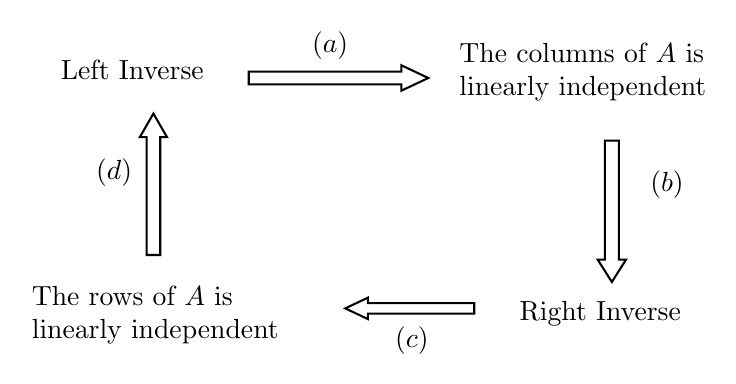
\begin{tikzpicture}[x=0.75pt,y=0.75pt,yscale=-1,xscale=1]
    %uncomment if require: \path (0,300); %set diagram left start at 0, and has height of 300

    %Right Arrow [id:dp1873650424277289] 
    \draw   (269,87.07) -- (342.52,87.07) -- (342.52,84) -- (355.52,90.14) -- (342.52,96.27) -- (342.52,93.2) -- (269,93.2) -- cycle ;
    %Right Arrow [id:dp6482140902579632] 
    \draw   (219.8,175.44) -- (219.8,118.66) -- (216.53,118.66) -- (223.08,107.27) -- (229.64,118.66) -- (226.36,118.66) -- (226.36,175.44) -- cycle ;
    %Right Arrow [id:dp31978358236465754] 
    \draw   (447.37,120.34) -- (447.37,177.66) -- (450.78,177.66) -- (443.96,188.43) -- (437.14,177.66) -- (440.55,177.66) -- (440.55,120.34) -- cycle ;
    %Right Arrow [id:dp9972986143574651] 
    \draw   (377.64,198.57) -- (326.37,198.57) -- (326.37,196) -- (315.52,201.14) -- (326.37,206.27) -- (326.37,203.7) -- (377.64,203.7) -- cycle ;

    % Text Node
    \draw (177,80) node [anchor=north west][inner sep=0.75pt]   [align=left] {Left Inverse};
    % Text Node
    \draw (369,72) node [anchor=north west][inner sep=0.75pt]   [align=left] {The columns of $A$ is\\ linearly independent};
    % Text Node
    \draw (163,189) node [anchor=north west][inner sep=0.75pt]   [align=left] {The rows of $A$ is\\ linearly independent};
    % Text Node
    \draw (398,196) node [anchor=north west][inner sep=0.75pt]   [align=left] {Right Inverse};
    % Text Node
    \draw (298,66.4) node [anchor=north west][inner sep=0.75pt]    {$( a)$};
    % Text Node
    \draw (338,208.4) node [anchor=north west][inner sep=0.75pt]    {$( c)$};
    % Text Node
    \draw (461,133.4) node [anchor=north west][inner sep=0.75pt]    {$( b)$};
    % Text Node
    \draw (194,127.4) node [anchor=north west][inner sep=0.75pt]    {$( d)$};


    \end{tikzpicture}

    \begin{itemize}
        \item 性质 $ (\mathrm{a}) $ 对任意矩阵 $ A \in \mathbb{R}^{m \times n} $ 都成立 
        \item 性质$(b)$对方阵矩阵 $ A \in \mathbb{R}^{n \times n} $ 都成立
        \item 对于性质 $ (\mathrm{c}) $ 与 $ (\mathrm{d}) $, 可利用 $ A^{T} $ 证明
    \end{itemize}
\end{proof}

\begin{theorem}
    $(a)$: $A$可左逆,则$A$列向量线性无关.
\end{theorem}

\begin{proof}
    假设$A$的左逆是 $ B $ ,则
    $$
    \begin{aligned}
            & A x=0 
     \Rightarrow &B A x=0 \\
    \Rightarrow & I x=0
    \end{aligned}
    $$

    假设A的列向量 $ A=\left[a_{1}, a_{2}, \cdots, a_{n}\right] $
    $$
    A x=x_{1} a_{1}+x_{2} a_{2}+\cdots+x_{n} a_{n}=0
    $$

    则当该等式 $ A x=0 $ 成立时,其解 $ x=0 $, 则A的列向量线性无关.  
    
    \begin{corollary}
        如果 $ A \in \mathbb{R}^{m \times n} $有左逆,则有 $ m \geq n = r $. 

    即$A$是高或方的矩阵, 如 $ A=\left[\begin{array}{ll}1 & 0 \\ 0 & 1 \\ 0 & 0\end{array}\right] $. 
    
    此时$A$的行向量可能线性相关,而$A$的列向量线性无关. $N(A) = \{0\}$.
    \end{corollary}
    

    假设 $ A $ 的列向量 $ A=\left[a_{1}, a_{2}, \cdots, a_{n}\right] $
    $$
    \begin{aligned}
         A x&=x_{1} a_{1}+x_{2} a_{2}+\cdots+x_{n} a_{n}=b \\
    A y&=y_{1} a_{1}+y_{2} a_{2}+\cdots+y_{n} a_{n}=b \\
    \end{aligned}
    $$

    $$A x-A y=A(x-y)=0 \Rightarrow x=y$$

    当 $ b \in \mathbb{R}^{m}, b \notin\left\{y \mid y=A x, x \in \mathbb{R}^{n}\right\} $ 时(即$b$不在$A$的列空间,$ m \geq n  $时),线性方程组无解.  $ A x=b $ 至多一个解,如有解则 $ x=X b $ . 
\end{proof}

\begin{theorem}
    矩阵的行秩等于列秩.
\end{theorem}

\begin{proof}
    令 $A$ 是一个 $m\times n$ 的矩阵,其列秩为 $r $. 因此矩阵 $A$ 的列空间的维度是 $r$ . 
    
    令 $c_1,c_2,\ldots,c_r$ 是 $A$ 的列空间的一组基,构成 $m \times r$ 矩阵 $C$ 的列向量 $C = [c_1,c_2,\ldots,c_r]$,并使得 $A$ 的每个列向量是 $C$ 的 $r$ 个列向量的线性组合. 
    
    由矩阵乘法的定义,存在一个 $r \times n$ 矩阵 $R$, 使得 $A = CR$. ($A$ 的 $(i,j)$ 元素是 $c_i$ 与 $R$ 的第 $j$ 个行向量的点积.)

现在,由于 $A = CR$, $A$ 的每个行向量是 $R$ 的行向量的线性组合,这意味着 $A$ 的行向量空间被包含于 $R$ 的行向量空间之中. 因此 $A 的行秩 \leq R的行秩$. 但$R$仅有$r$行, 所以$R的行秩 \leq r = A的列秩$. 这就证明了$A的行秩 \leq A的列秩$.

把上述证明过程中的“行”与“列”交换,利用对偶性质同样可证$A的列秩 \leq A的行秩$. 更简单的方法是考虑A的转置矩阵 $A^\mathrm{T}$,则$A的列秩 =  A^\mathrm{T}的行秩 \leq  A^\mathrm{T}的列秩 = A的行秩$. 这证明了$A$的列秩等于$A$的行秩. 证毕.
\end{proof}

\begin{theorem}
    $(c)$: 矩阵 $ A \in \mathbb{R}^{m \times n} $ 有右逆 $ X $, 则A行向量线性无关.
\end{theorem}

\begin{proof}
    $$ \mathrm{X}^{T} A^{T}=(A X)^{T}=I $$
    
    则有 $ \mathrm{X}^{T} $ 是 $ A^{T} $ 的左逆, $ A^{T} $ 的列向量线性无关.  

    即 $ A^{T} \in \mathbb{R}^{n \times m} $.
    
    \begin{corollary}
     如果 $ A \in \mathbb{R}^{m \times n} $有左逆,则有 $r= m \leq n  $. 

    即$A$是宽或方的矩阵. 

    此时$A$的列向量可能线性相关,而$A$的行向量线性无关. 
    
    $N(A^T) = \{0\}, \operatorname{dim} N(A) = n-r, r=m$. ($Ax=b$有无穷解) 
    \end{corollary}
    
    根据定理“矩阵的行秩等于列秩”,$ A^{T} $ 的列向量线性无关,则矩阵 $ A $ 有$m$个线性无关列向量(行向量),即通过 Gram-Schmidt 正交化可得$m$个正交基. 

    $ \forall b \in \mathbb{R}^{m} $, 有 $ b \in\left\{y \mid y=A x, x \in \mathbb{R}^{n}\right\} (m \leq n ) $, 方程 $ A x=b $ 有解,其解为 $ x=X b $ . 
\end{proof}

\begin{theorem}
    $(b)$: 若方阵A列向量线性无关,则A可右逆. 
\end{theorem}

\begin{proof}
    假设 $ A \in \mathbb{R}^{n \times n} $ 为方阵且列向量线性无关 
    
    $$ A=\left[a_{1}, a_{2}, \cdots, a_{n}\right] $$

    则对于任意向量 $ \mathrm{b} \in \mathbb{R}^{n} $, 则向量组 $ \left[a_{1}, a_{2}, \ldots, a_{n}, \mathrm{~b}\right] $ 线性相关,存 在不全为0的系数,使得以下等式成立
    $$
    x_{1} a_{1}+x_{2} a_{2}+\cdots+x_{n} a_{n}+x_{n+1} b=0
    $$

    因为$A$列向量线性无关,则 $ x_{n+1} \neq 0 $(假设$ x_{n+1} = 0 $会推出违反线性无关假设的结论), 即$b$是$A$列向量的线性组合;
    $$
    b=-\frac{x_{1}}{x_{n+1}} a_{1}-\frac{x_{2}}{x_{n+1}} a_{2}-\cdots-\frac{x_{n}}{x_{n+1}} a_{n}
    $$

    存在向量 $ c_{1}, \ldots, c_{n} \in \mathbb{R}^{n} $,使得 
    $$
    \begin{aligned}
        Ac _{1}&=e_{1}\\
         A c_{2}&=e_{2}\\
          \ldots \\
          A c_{n}&=e_{n}
    \end{aligned}
    $$

    则矩阵 $ C=\left[c_{1} c_{2} \ldots c_{n}\right] $ 是矩阵 $ A $ 的右逆, $ A C=I $.

\end{proof}

\section{转置和共轭转置的逆}

\begin{theorem}[转置 $ A^{T} $ 和共轭转置 $ A^{\mathrm{H}} $ ]
    如果矩阵$A$为非奇异矩阵,则其转置 $ A^{T} $ 和共轭转置 $ A^{\mathrm{H}} $ 都为非奇异矩阵,则有
$$
\begin{array}{l}
\left(A^{T}\right)^{-1}=\left(A^{-1}\right)^{T}, \quad\left(A^{H}\right)^{-1}=\left(A^{-1}\right)^{H} \\
\end{array}
$$
\end{theorem}

\begin{proof}
    $$\left(A A^{-1}\right)^{T}=I \Rightarrow \underbrace{\left(A^{-1}\right)^{T}}_{\text{the inverse of }A^T}   A^{T}=I$$
\end{proof}

\begin{corollary}
    如果矩阵A和矩阵B都为非奇异矩阵,则乘积AB也为非 奇异矩阵
$$
\begin{array}{l}
(A B)^{-1}=B^{-1} A^{-1} \\
\end{array}
$$
\end{corollary}

\begin{proof}
    $$(A B) \underbrace{B^{-1} A^{-1}} _{\text{the inverse of AB}}=I$$
\end{proof}

\section{Gram Matrix非奇异的性质}

\label{Sect:GramNonSingular}

Gram矩阵的定义见 \ref{Def:Gram}.

\begin{corollary}[Gram Matrix 可逆等价于$A$列线性无关]
    矩阵 $ A \in \mathbb{R}^{m \times n},  \mathrm{G}=A^{T} A $

矩阵 $ A $ 列向量线性无关 $ \Leftrightarrow $ Gram矩阵G非奇异.
\end{corollary}

\begin{proof}
    " $ \Rightarrow $ ": 
    
    假设矩阵 $ A $ 列向量线性无关, $ A^{T} A $ 奇异.  则存在 $ A^{T} A x=0, x \neq 0 $, 可得 $ x^{T} A^{T} A x=\|A x\|_{2}^{2}=0 $, 即 $ A x=0 $ 与列向量线性无矛盾.

    " $ \Leftarrow $ ":
    
    假设 $ A^{T} A $ 非奇异, 矩阵 $ A $ 列向量线性相关.  则有 $ A x=0, x \neq 0 $, 可得 $ A^{T} A x=0 $, 即 $ A^{T} A $ 是奇异矩阵. 
\end{proof}

\section{伪逆}

\begin{definition}[Pseudo-inverse]
    $$ A^{\dagger}=A^{T}\left(A A^{T}\right)^{-1} $$

    $$A^{\dagger} = V \Sigma^+ U^T = \left[v_{1} \cdots v_{r} \cdots v_{n}\right]\left[\begin{array}{lll}
        \sigma_{1}^{-1} & & \\
        & \ddots & \\
        & & \sigma_{r}^{-1}
        \end{array}\right]\left[u_{1} \cdots u_{r} \cdots u_{m}\right]^{\mathrm{T}}$$
\end{definition}

\begin{theorem}
    伪逆 $ A^{\dagger} $ 为 $ A $ 的右逆
\end{theorem}

\begin{proof}
    $$ A A^{\dagger}=A A^{T}\left(A A^{T}\right)^{-1}=\left(A A^{T}\right)^{-1}\left(A A^{T}\right)=I $$
\end{proof}

\begin{theorem}
    当$A$为方阵时,右逆等于矩阵的逆
\end{theorem}

\begin{proof}
    $$ A^{\dagger}=A^{T}\left(A A^{T}\right)^{-1}=A^{T} A^{-T} A^{-1}=A^{-1} $$
\end{proof}

\begin{theorem}
    
\end{theorem}

\begin{corollary}
    以下三个结论为等价的,对于实矩阵$A$

    \begin{itemize}
        \item $A$是可左逆的
        \item $A$的列向量线性无关
        \item $ A^{T} A $ 为非奇异矩阵
    \end{itemize}
\end{corollary}

\begin{corollary}
    以下三个结论为等价的,对于实矩阵$A$

    \begin{itemize}
        \item $A$是可右逆的 
        \item $A$的行向量线性无关
        \item $ A A^{T} $ 为非奇异矩阵
    \end{itemize}
\end{corollary}

By choosing good bases, $A$ multiplies $\boldsymbol{v}_{i}$ in the row space to give $\sigma_{i} \boldsymbol{u}_{i}$ in the column space. $A^{-1}$ must do the opposite! 



If $A \boldsymbol{v}=\sigma \boldsymbol{u}$ then $A^{-1} \boldsymbol{u}=\boldsymbol{v} / \sigma$. The singular values of $A^{-1}$ are $1 / \sigma$, just as the eigenvalues of $A^{-1}$ are $1 / \lambda$. The bases are reversed. The $u$ 's are in the row space of $A^{-1}$, the $v$ 's are in the column space.

The pseudoinverse $A^{+}$is an $n$ by $m$ matrix. \textbf{If $A^{-1}$ exists, then $A^{+}$is the same as $A^{-1}$}. In that case $m=n=r$ and we are inverting $U \Sigma V^{\mathrm{T}}$ to get $V \Sigma^{-1} U^{\mathrm{T}}$. 

The new symbol $A^{+}$is needed when $r<m$ or $r<n$. Then $A$ has no two-sided inverse, but it has a \textit{pseudo}inverse $A^{+}$with that same rank $r$ :

$$
A^{+} \boldsymbol{u}_{i}=\frac{1}{\sigma_{i}} \boldsymbol{v}_{i} \quad \text { for } i \leq r \quad \text { and } \quad A^{+} \boldsymbol{u}_{i}=\mathbf{0} \quad \text { for } i>r
$$

The vectors $\boldsymbol{u}_{1}, \ldots, \boldsymbol{u}_{r}$ in the column space of $A$ go back to $\boldsymbol{v}_{1}, \ldots, \boldsymbol{v}_{r}$ in the row space.


The other vectors $\boldsymbol{u}_{r+1}, \ldots, \boldsymbol{u}_{m}$ are in the left nullspace, and $A^{+}$sends them to zero. When we know what happens to all those basis vectors, we know $A^{+}$.

Notice the pseudoinverse of the diagonal matrix $\Sigma .$ Each $\sigma$ in $\Sigma$ is replaced by $\sigma^{-1}$ in $\Sigma^{+} .$The product $\Sigma^{+} \Sigma$ is as near to the identity as we can get. It is a projection matrix, $\Sigma^{+} \Sigma$ is partly $I$ and otherwise zero. We can invert the $\sigma$ 's, but we can't do anything about the zero rows and columns. 

\begin{FigureCenter}{$ A \boldsymbol{x}^{\dagger} $ in the column space goes back to $ A^{\dagger} A \boldsymbol{x}^{\dagger}=\boldsymbol{x}^{\dagger}$ in the row space}
    

    \tikzset{every picture/.style={line width=0.75pt}} %set default line width to 0.75pt        
    
    \begin{tikzpicture}[x=0.75pt,y=0.75pt,yscale=-1,xscale=1]
    %uncomment if require: \path (0,457); %set diagram left start at 0, and has height of 457
    
    %Shape: Rectangle [id:dp8596899930926358] 
    \draw  [dash pattern={on 0.84pt off 2.51pt}] (412.64,146.65) -- (440.94,174.46) -- (412.24,203.67) -- (383.93,175.86) -- cycle ;
    %Shape: Rectangle [id:dp144129295466213] 
    \draw   (159.81,65.14) -- (236.34,135.27) -- (193.59,181.93) -- (117.06,111.79) -- cycle ;
    %Shape: Rectangle [id:dp4244539260616451] 
    \draw   (193.59,181.93) -- (260.03,242.81) -- (218.64,287.99) -- (152.2,227.1) -- cycle ;
    
    %Shape: Rectangle [id:dp10811540545272225] 
    \draw   (477.03,51.53) -- (398.27,133.34) -- (440.51,174) -- (519.26,92.19) -- cycle ;
    %Shape: Rectangle [id:dp952165170642489] 
    \draw   (440.51,174) -- (372.14,245.02) -- (413.05,284.39) -- (481.41,213.38) -- cycle ;
    
    %Straight Lines [id:da43480021093829335] 
    \draw [color={rgb, 255:red, 139; green, 87; blue, 42 }  ,draw opacity=1 ][line width=2.25]    (193.59,181.93) -- (187.34,138.27) ;
    \draw [shift={(186.64,133.33)}, rotate = 441.85] [fill={rgb, 255:red, 139; green, 87; blue, 42 }  ,fill opacity=1 ][line width=0.08]  [draw opacity=0] (8.57,-4.12) -- (0,0) -- (8.57,4.12) -- cycle    ;
    %Straight Lines [id:da6356667569876433] 
    \draw [color={rgb, 255:red, 245; green, 166; blue, 35 }  ,draw opacity=1 ][line width=2.25]    (440.51,175) -- (415.75,200.11) ;
    \draw [shift={(412.24,203.67)}, rotate = 314.6] [fill={rgb, 255:red, 245; green, 166; blue, 35 }  ,fill opacity=1 ][line width=0.08]  [draw opacity=0] (8.57,-4.12) -- (0,0) -- (8.57,4.12) -- cycle    ;
    %Straight Lines [id:da22563123154133025] 
    \draw [color={rgb, 255:red, 65; green, 117; blue, 5 }  ,draw opacity=1 ][line width=2.25]    (440.51,175) -- (388.93,175.78) ;
    \draw [shift={(383.93,175.86)}, rotate = 359.13] [fill={rgb, 255:red, 65; green, 117; blue, 5 }  ,fill opacity=1 ][line width=0.08]  [draw opacity=0] (8.57,-4.12) -- (0,0) -- (8.57,4.12) -- cycle    ;
    %Shape: Rectangle [id:dp12172823301153524] 
    \draw   (186.5,176.41) -- (193.59,182.93) -- (186.84,190.28) -- (179.74,183.76) -- cycle ;
    %Shape: Rectangle [id:dp9349834759264539] 
    \draw   (447.27,167.65) -- (454.36,174.17) -- (447.61,181.52) -- (440.51,175) -- cycle ;
    %Straight Lines [id:da2510398254796229] 
    \draw [color={rgb, 255:red, 108; green, 108; blue, 215 }  ,draw opacity=1 ][line width=2.25]    (440.51,175) -- (416.14,150.21) ;
    \draw [shift={(412.64,146.65)}, rotate = 405.49] [fill={rgb, 255:red, 108; green, 108; blue, 215 }  ,fill opacity=1 ][line width=0.08]  [draw opacity=0] (8.57,-4.12) -- (0,0) -- (8.57,4.12) -- cycle    ;
    %Straight Lines [id:da5471202445204062] 
    \draw  [dash pattern={on 4.5pt off 4.5pt}]  (383.93,175.86) -- (186.64,133.33) ;
    \draw [shift={(285.28,154.59)}, rotate = 372.15999999999997] [fill={rgb, 255:red, 0; green, 0; blue, 0 }  ][line width=0.08]  [draw opacity=0] (8.93,-4.29) -- (0,0) -- (8.93,4.29) -- cycle    ;
    %Straight Lines [id:da12114390650727058] 
    \draw  [dash pattern={on 4.5pt off 4.5pt}]  (412.64,146.65) -- (186.64,133.33) ;
    \draw [shift={(299.64,139.99)}, rotate = 363.37] [fill={rgb, 255:red, 0; green, 0; blue, 0 }  ][line width=0.08]  [draw opacity=0] (8.93,-4.29) -- (0,0) -- (8.93,4.29) -- cycle    ;
    %Straight Lines [id:da8219115744539653] 
    \draw  [dash pattern={on 4.5pt off 4.5pt}]  (412.24,203.67) -- (193.59,181.93) ;
    \draw [shift={(302.92,192.8)}, rotate = 365.68] [fill={rgb, 255:red, 0; green, 0; blue, 0 }  ][line width=0.08]  [draw opacity=0] (8.93,-4.29) -- (0,0) -- (8.93,4.29) -- cycle    ;
    
    % Text Node
    \draw (9,64) node [anchor=north west][inner sep=0.75pt]   [align=left] {Row Space $\displaystyle A^{T} y$\\dim $\displaystyle r$};
    % Text Node
    \draw (16,217) node [anchor=north west][inner sep=0.75pt]   [align=left] {Nullspace $\displaystyle Ax=0$\\dim $\displaystyle n-r$};
    % Text Node
    \draw (506,32) node [anchor=north west][inner sep=0.75pt]   [align=left] {Column Space $\displaystyle Ax$\\dim $\displaystyle r$};
    % Text Node
    \draw (469,224) node [anchor=north west][inner sep=0.75pt]   [align=left] {Left Nullspace $\displaystyle A^{T} y=0$\\dim $\displaystyle m-r$};
    % Text Node
    \draw (173,114.4) node [anchor=north west][inner sep=0.75pt]  [color={rgb, 255:red, 139; green, 87; blue, 42 }  ,opacity=1 ]  {$x^{\dagger }$};
    % Text Node
    \draw (417,202.4) node [anchor=north west][inner sep=0.75pt]  [color={rgb, 255:red, 245; green, 166; blue, 35 }  ,opacity=1 ]  {$e$};
    % Text Node
    \draw (423,132.4) node [anchor=north west][inner sep=0.75pt]  [color={rgb, 255:red, 108; green, 108; blue, 215 }  ,opacity=1 ]  {$p$};
    % Text Node
    \draw (370,167.4) node [anchor=north west][inner sep=0.75pt]  [color={rgb, 255:red, 65; green, 117; blue, 5 }  ,opacity=1 ]  {$b$};
    % Text Node
    \draw (473,153.4) node [anchor=north west][inner sep=0.75pt]  [color={rgb, 255:red, 108; green, 108; blue, 215 }  ,opacity=1 ]  {$ \begin{array}{l}
    \textcolor[rgb]{0.42,0.42,0.84}{p}\textcolor[rgb]{0,0,0}{=A}\textcolor[rgb]{0.55,0.34,0.16}{x}\textcolor[rgb]{0.55,0.34,0.16}{^{\dagger }}\\
    \textcolor[rgb]{0,0,0}{=AA}\textcolor[rgb]{0,0,0}{^{\dagger }}\textcolor[rgb]{0.25,0.46,0.02}{b}\\
    \end{array}$};
    % Text Node
    \draw (276,197.4) node [anchor=north west][inner sep=0.75pt]    {$A^{\dagger } e=0$};
    % Text Node
    \draw (241,160.4) node [anchor=north west][inner sep=0.75pt]    {$A^{\dagger }\textcolor[rgb]{0.25,0.46,0.02}{b} =\textcolor[rgb]{0.55,0.34,0.16}{x}\textcolor[rgb]{0.55,0.34,0.16}{^{\dagger }}$};
    % Text Node
    \draw (287,113.4) node [anchor=north west][inner sep=0.75pt]    {$A^{\dagger }\textcolor[rgb]{0.42,0.42,0.84}{p} =\textcolor[rgb]{0.55,0.34,0.16}{x}\textcolor[rgb]{0.55,0.34,0.16}{^{\dagger }}$};
    % Text Node
    \draw  [color={rgb, 255:red, 0; green, 0; blue, 0 }  ,draw opacity=0 ][fill={rgb, 255:red, 249; green, 192; blue, 139 }  ,fill opacity=1 ][dash pattern={on 0.84pt off 2.51pt}]  (208,43) .. controls (208,40.24) and (210.24,38) .. (213,38) -- (418,38) .. controls (420.76,38) and (423,40.24) .. (423,43) -- (423,83) .. controls (423,85.76) and (420.76,88) .. (418,88) -- (213,88) .. controls (210.24,88) and (208,85.76) .. (208,83) -- cycle  ;
    \draw (211,42.4) node [anchor=north west][inner sep=0.75pt]    {$A^{\dagger } A=\begin{bmatrix}
    I & 0\\
    0 & 0
    \end{bmatrix} \ \begin{matrix}
    (\text{row\ space})\\
    (\text{nullspace})
    \end{matrix}$};
    % Text Node
    \draw (122,133) node [anchor=north west][inner sep=0.75pt]   [align=left] {text};
    % Text Node
    \draw  [color={rgb, 255:red, 0; green, 0; blue, 0 }  ,draw opacity=0 ][fill={rgb, 255:red, 249; green, 192; blue, 139 }  ,fill opacity=1 ]  (191,307) .. controls (191,304.24) and (193.24,302) .. (196,302) -- (443,302) .. controls (445.76,302) and (448,304.24) .. (448,307) -- (448,347) .. controls (448,349.76) and (445.76,352) .. (443,352) -- (196,352) .. controls (193.24,352) and (191,349.76) .. (191,347) -- cycle  ;
    \draw (194,306.4) node [anchor=north west][inner sep=0.75pt]    {$\begin{matrix}
    A & \text{Row\ space\ to\ column\ space}\\
    A^{\dagger } & \text{Column\ space\ to\ row\ space}
    \end{matrix}$};
    
    
    \end{tikzpicture}
    \end{FigureCenter}

\begin{FigureCenter}{Projection from row space to column space}
    

\tikzset{every picture/.style={line width=0.75pt}} %set default line width to 0.75pt        

\begin{tikzpicture}[x=0.75pt,y=0.75pt,yscale=-1,xscale=1]
%uncomment if require: \path (0,376); %set diagram left start at 0, and has height of 376

%Shape: Rectangle [id:dp8564537788335302] 
\draw  [dash pattern={on 0.84pt off 2.51pt}] (221.63,153.4) -- (253.96,185.17) -- (225.93,213.7) -- (193.59,181.93) -- cycle ;
%Shape: Rectangle [id:dp7748103688398633] 
\draw   (159.81,65.14) -- (236.34,135.27) -- (193.59,181.93) -- (117.06,111.79) -- cycle ;
%Shape: Rectangle [id:dp3534850306924755] 
\draw   (193.59,181.93) -- (260.03,242.81) -- (218.64,287.99) -- (152.2,227.1) -- cycle ;

%Shape: Rectangle [id:dp11468847928918202] 
\draw   (477.03,52.53) -- (398.27,134.34) -- (440.51,175) -- (519.26,93.19) -- cycle ;
%Shape: Rectangle [id:dp8320016424104848] 
\draw   (440.51,175) -- (372.14,246.02) -- (413.05,285.39) -- (481.41,214.38) -- cycle ;

%Straight Lines [id:da413550032058265] 
\draw [color={rgb, 255:red, 139; green, 87; blue, 42 }  ,draw opacity=1 ][line width=2.25]    (193.59,181.93) -- (217.74,155.81) ;
\draw [shift={(221.14,152.14)}, rotate = 492.75] [fill={rgb, 255:red, 139; green, 87; blue, 42 }  ,fill opacity=1 ][line width=0.08]  [draw opacity=0] (8.57,-4.12) -- (0,0) -- (8.57,4.12) -- cycle    ;
%Straight Lines [id:da05215716031511208] 
\draw [color={rgb, 255:red, 245; green, 166; blue, 35 }  ,draw opacity=1 ][line width=2.25]    (193.59,181.93) -- (222.99,209.56) ;
\draw [shift={(226.64,212.99)}, rotate = 223.23] [fill={rgb, 255:red, 245; green, 166; blue, 35 }  ,fill opacity=1 ][line width=0.08]  [draw opacity=0] (8.57,-4.12) -- (0,0) -- (8.57,4.12) -- cycle    ;
%Straight Lines [id:da20598638562684246] 
\draw [color={rgb, 255:red, 65; green, 117; blue, 5 }  ,draw opacity=1 ][line width=2.25]    (193.59,181.93) -- (248.97,184.9) ;
\draw [shift={(253.96,185.17)}, rotate = 183.08] [fill={rgb, 255:red, 65; green, 117; blue, 5 }  ,fill opacity=1 ][line width=0.08]  [draw opacity=0] (8.57,-4.12) -- (0,0) -- (8.57,4.12) -- cycle    ;
%Straight Lines [id:da9574000480451021] 
\draw  [dash pattern={on 4.5pt off 4.5pt}]  (221.14,152.14) -- (435.64,119.99) ;
\draw [shift={(328.39,136.06)}, rotate = 531.48] [fill={rgb, 255:red, 0; green, 0; blue, 0 }  ][line width=0.08]  [draw opacity=0] (8.93,-4.29) -- (0,0) -- (8.93,4.29) -- cycle    ;
%Straight Lines [id:da8574440156945131] 
\draw  [dash pattern={on 4.5pt off 4.5pt}]  (253.96,185.17) -- (435.64,119.99) ;
\draw [shift={(344.8,152.58)}, rotate = 520.26] [fill={rgb, 255:red, 0; green, 0; blue, 0 }  ][line width=0.08]  [draw opacity=0] (8.93,-4.29) -- (0,0) -- (8.93,4.29) -- cycle    ;
%Straight Lines [id:da26442247252775863] 
\draw  [dash pattern={on 4.5pt off 4.5pt}]  (226.64,212.99) -- (440.51,175) ;
\draw [shift={(333.57,193.99)}, rotate = 529.9300000000001] [fill={rgb, 255:red, 0; green, 0; blue, 0 }  ][line width=0.08]  [draw opacity=0] (8.93,-4.29) -- (0,0) -- (8.93,4.29) -- cycle    ;
%Shape: Rectangle [id:dp41111107193098295] 
\draw   (186.5,176.41) -- (193.59,182.93) -- (186.84,190.28) -- (179.74,183.76) -- cycle ;
%Shape: Rectangle [id:dp37902094791189933] 
\draw   (447.27,167.65) -- (454.36,174.17) -- (447.61,181.52) -- (440.51,175) -- cycle ;
%Straight Lines [id:da3897829543263125] 
\draw [color={rgb, 255:red, 108; green, 108; blue, 215 }  ,draw opacity=1 ][line width=2.25]    (440.51,175) -- (436.08,124.97) ;
\draw [shift={(435.64,119.99)}, rotate = 444.94] [fill={rgb, 255:red, 108; green, 108; blue, 215 }  ,fill opacity=1 ][line width=0.08]  [draw opacity=0] (8.57,-4.12) -- (0,0) -- (8.57,4.12) -- cycle    ;

% Text Node
\draw (10,62) node [anchor=north west][inner sep=0.75pt]   [align=left] {Row Space $\displaystyle A^{T} y$\\dim $\displaystyle r$};
% Text Node
\draw (22,240) node [anchor=north west][inner sep=0.75pt]   [align=left] {Nullspace $\displaystyle Ax=0$\\dim $\displaystyle n-r$};
% Text Node
\draw (510,39) node [anchor=north west][inner sep=0.75pt]   [align=left] {Column Space $\displaystyle Ax$\\dim $\displaystyle r$};
% Text Node
\draw (462,245) node [anchor=north west][inner sep=0.75pt]   [align=left] {Left Nullspace $\displaystyle A^{T} y=0$\\dim $\displaystyle m-r$};
% Text Node
\draw (291,112.4) node [anchor=north west][inner sep=0.75pt]    {$A\textcolor[rgb]{0.55,0.34,0.16}{x}\textcolor[rgb]{0.55,0.34,0.16}{_{r}} =\textcolor[rgb]{0.42,0.42,0.84}{b}$};
% Text Node
\draw (202,136.4) node [anchor=north west][inner sep=0.75pt]  [color={rgb, 255:red, 139; green, 87; blue, 42 }  ,opacity=1 ]  {$x_{r}$};
% Text Node
\draw (207,210.4) node [anchor=north west][inner sep=0.75pt]  [color={rgb, 255:red, 245; green, 166; blue, 35 }  ,opacity=1 ]  {$x_{n}$};
% Text Node
\draw (443,111.4) node [anchor=north west][inner sep=0.75pt]  [color={rgb, 255:red, 108; green, 108; blue, 215 }  ,opacity=1 ]  {$b$};
% Text Node
\draw (331,158.4) node [anchor=north west][inner sep=0.75pt]    {$A\textcolor[rgb]{0.25,0.46,0.02}{x} =\textcolor[rgb]{0.42,0.42,0.84}{b}$};
% Text Node
\draw (301,202.4) node [anchor=north west][inner sep=0.75pt]    {$A\textcolor[rgb]{0.96,0.65,0.14}{x}\textcolor[rgb]{0.96,0.65,0.14}{_{n}} =0$};
% Text Node
\draw (250,164.4) node [anchor=north west][inner sep=0.75pt]  [color={rgb, 255:red, 65; green, 117; blue, 5 }  ,opacity=1 ]  {$x$};
% Text Node
\draw  [color={rgb, 255:red, 0; green, 0; blue, 0 }  ,draw opacity=0 ][fill={rgb, 255:red, 249; green, 192; blue, 139 }  ,fill opacity=1 ]  (191,305) .. controls (191,302.24) and (193.24,300) .. (196,300) -- (443,300) .. controls (445.76,300) and (448,302.24) .. (448,305) -- (448,345) .. controls (448,347.76) and (445.76,350) .. (443,350) -- (196,350) .. controls (193.24,350) and (191,347.76) .. (191,345) -- cycle  ;
\draw (194,304.4) node [anchor=north west][inner sep=0.75pt]    {$\begin{matrix}
A & \text{Row\ space\ to\ column\ space}\\
A^{\dagger } & \text{Column\ space\ to\ row\ space}
\end{matrix}$};


\end{tikzpicture}
\end{FigureCenter}
\chapter{Orthogonal Matrices}

\section{预备知识}

\subsection{标准正交向量}

参见 \ref{Def:OrthonormalVectors}。

\subsection{Gram 矩阵与标准正交的关系}

For the definition of Gram matrices, refer to \ref{Def:Gram}. 关于它与非奇异的性质,参见 \ref{Sect:GramNonSingular}.

\begin{theorem}
    如果A的Gram矩阵为单位矩阵,则 $ A \in \mathbb{R}^{m \times n} $ 具有标准正交列.
\end{theorem}

\begin{proof}
    $$ \begin{aligned} A^{T} A&=\left[\begin{array}{llll}a_{1} & a_{2} & \cdots & a_{n}\end{array}\right]^{T}\left[\begin{array}{llll}a_{1} & a_{2} & \cdots & a_{n}\end{array}\right] 
    \\ &=\left[\begin{array}{cccc}a_{1}^{T} a_{1} & a_{1}^{T} a_{2} & \cdots & a_{1}{ }^{T} a_{n} \\ a_{2}^{T} a_{1} & a_{2}{ }^{T} a_{2} & \cdots & a_{2}^{T} a_{n} \\ \vdots & \vdots & \ddots & \vdots \\ a_{n}^{T} a_{1} & a_{n}^{T} a_{2} & \cdots & a_{n}^{T} a_{n}\end{array}\right] 
    \\  &=\left[\begin{array}{cccc}1 & 0 & \cdots & 0 \\ 0 & 1 & \cdots & 0 \\ \vdots & \vdots & \ddots & \vdots \\ 0 & 0 & \cdots & 1\end{array}\right] 
    \\ & =I  \end{aligned} $$
\end{proof}

\subsection{矩阵-向量乘积与标准正交的关系}

如果 $ A \in \mathbb{R}^{m \times n} $ 具有标准正交列,则线性函数 $ f(x)=A x $

\begin{theorem}
    保持原内积.
    $$ \langle A x, A y\rangle=x^{T} y $$
\end{theorem}

\begin{proof}
    $$ \langle A x, A y\rangle=(A x)^{T}(A y)=x^{T} A^{T} A y=x^{T} y $$
\end{proof}


\begin{theorem}
    保持原范数.
    $$
    \|A x\|_{2}=\|x\|_{2}
    $$
\end{theorem}

\begin{proof}
   $$
\|A x\|_{2}=\left((A x)^{T}(A x)\right)^{1 / 2}=\left(x^{T} x\right)^{1 / 2}=\|x\|_{2}
$$
\end{proof}

\begin{theorem}
    保持原距离.

    $$
    \|A x-A y\|_{2}=\|x-y\|_{2}
    $$
\end{theorem}

\begin{proof}
   $$
\|A x-A y\|_{2}=\left((A x-A y)^{T}(A x-A y)\right)^{1 / 2}=\left((x-y)^{T}(x-y)\right)^{1 / 2}=\|x-y\|_{2}
$$
\end{proof}

\begin{theorem}
    保持原角度.

    $$ \angle(A x, A y)=\angle(x, y) $$
\end{theorem}

\begin{proof}
    $$ \angle(A x, A y)=\arccos \left(\frac{(A x)^{T}(A y)}{\|A x\|_{2}\|A y\|_{2}}\right)=\arccos \left(\frac{x^{T} y}{\|x\|_{2}\|y\|_{2}}\right)=\angle(x, y) $$
\end{proof}

\subsection{左可逆性与正交的关系}


如果矩阵 $ A \in \mathbb{R}^{m \times n} $ 有标准正交列,则:

\begin{theorem}
    $ A $ 是左可逆的,其左逆为 $ A^{T} $.
\end{theorem}

\begin{proof}
    根据定义:

$$
A^{T} A=I
$$
\end{proof}

\begin{theorem}
    $ A $ 有线性无关的列向量.
\end{theorem}

\begin{proof}
    $$
A x=0 \quad \Rightarrow \quad A^{T} A x=x=0
$$
\end{proof}

\begin{theorem}
    $A$ 是高的或者方的, 即 $m \geq n$.
\end{theorem}

\begin{proof}
    列向量 $ a_{1}, a_{2}, \ldots, a_{n} \in \mathbb{R}^{m} $, 由维度定理可得 $ n \leq m $。
\end{proof}

\section{正交矩阵}

\begin{definition}[正交矩阵]
    所有列两两相互正交的\textbf{方形}实矩阵。
\end{definition}

\begin{theorem}
    正交矩阵满足非奇异性.
    
    即如果矩阵 $ A $ 是正交的,则$ A $ 是可逆的,左逆等于右逆,且它的逆为 $ A^{T} $.

    $$ \left.\begin{array}{l}A^{T} A=I \\ A \text { 是方的 }\end{array}\right\} \quad \Rightarrow \quad A A^{T}=I $$
\end{theorem}

\begin{corollary}
    $ A^{T} $ 也是一个正交矩阵。
\end{corollary}

\begin{corollary}
    $ A $ 的行是标准正交的,即范数为1且相互正交。
\end{corollary}

\begin{remark}
    如果 $ A \in \mathbb{R}^{m \times n} $ 有标准正交列以及 $ m>n $, 则 $ A A^{T} \neq I_{\text {。 }} $
\end{remark}

\section{Permutation Matrices}

\begin{notation}
    $ \pi=\left(\pi_{1}, \pi_{2}, \ldots, \pi_{n}\right) $ 为 $ (1,2, \ldots, n) $ 的一个重新排序的排列。

    将 $ \pi $ 与一个置换矩阵 $ A \in \mathbb{R}^{n \times n} $ 联系起来:
$$
A_{i \pi_{i}}=1, \quad A_{i j}=0 \text { 如果 } j \neq \pi_{i}
$$
\end{notation}

\begin{definition}[置换]
    $ A x $ 是 $ x $ 的一个置换:
    
    $$ A x=\left(x_{\pi_{1}}, x_{\pi_{2}}, \ldots, x_{\pi_{n}}\right) $$
\end{definition}

$A$在每一行和每一列中都有一个等于1的元素。

\begin{theorem}
    置换矩阵满足正交性,即所有置换矩阵都是正交的.
\end{theorem}

\begin{corollary}
    $$ A^{T} A=I $$
\end{corollary}

\begin{proof}
    因为A的每一行有一个元素等于1
$$
\left(A^{T} A\right)_{i j}=\sum_{k=1}^{n} A_{k i} A_{k j}=\left\{\begin{array}{ll}
1 & i=j \\
0 & \text { 其它 }
\end{array}\right.
$$
\end{proof}

\begin{corollary}
    $ A^{T}=A^{-1} $是逆置换矩阵.
\end{corollary}

\begin{example}
    若 $ \{1,2,3,4\} $ 的置换为:
$$
\left(\pi_{1}, \pi_{2}, \pi_{3}, \pi_{4}\right)=(2,4,1,3)
$$

相应的置换矩阵及其逆矩阵为

$$ A=\left[\begin{array}{llll}0 & 1 & 0 & 0 \\ 0 & 0 & 0 & 1 \\ 1 & 0 & 0 & 0 \\ 0 & 0 & 1 & 0\end{array}\right] , A^{-1}=A^{T}=\left[\begin{array}{llll}0 & 0 & 1 & 0 \\ 1 & 0 & 0 & 0 \\ 0 & 0 & 0 & 1 \\ 0 & 1 & 0 & 0\end{array}\right] $$

$ A^{T} $ 是与置换相关的置换矩阵

$$
\left(\tilde{\pi}_{1}, \tilde{\pi}_{2}, \tilde{\pi}_{3}, \tilde{\pi}_{4}\right)=(3,1,4,2)
$$
\end{example}

\section{平面旋转}



\tikzset{every picture/.style={line width=0.75pt}} %set default line width to 0.75pt        

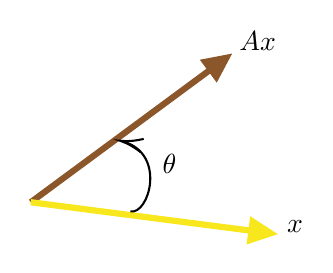
\begin{tikzpicture}[x=0.75pt,y=0.75pt,yscale=-1,xscale=1]
%uncomment if require: \path (0,300); %set diagram left start at 0, and has height of 300

%Straight Lines [id:da5121306887606891] 
\draw [color={rgb, 255:red, 139; green, 87; blue, 42 }  ,draw opacity=1 ][line width=2.25]    (100,112) -- (192.99,43.35) ;
\draw [shift={(197.01,40.38)}, rotate = 503.56] [fill={rgb, 255:red, 139; green, 87; blue, 42 }  ,fill opacity=1 ][line width=0.08]  [draw opacity=0] (14.29,-6.86) -- (0,0) -- (14.29,6.86) -- cycle    ;
%Straight Lines [id:da027572763792303556] 
\draw [color={rgb, 255:red, 248; green, 231; blue, 28 }  ,draw opacity=1 ][fill={rgb, 255:red, 248; green, 231; blue, 28 }  ,fill opacity=1 ][line width=2.25]    (100,112) -- (214.05,126.74) ;
\draw [shift={(219.01,127.38)}, rotate = 187.36] [fill={rgb, 255:red, 248; green, 231; blue, 28 }  ,fill opacity=1 ][line width=0.08]  [draw opacity=0] (14.29,-6.86) -- (0,0) -- (14.29,6.86) -- cycle    ;
%Curve Lines [id:da28950702982590015] 
\draw    (148.01,116.38) .. controls (156.78,118.33) and (165.56,88.91) .. (144.67,82.8) ;
\draw [shift={(143.01,82.38)}, rotate = 372.26] [color={rgb, 255:red, 0; green, 0; blue, 0 }  ][line width=0.75]    (10.93,-3.29) .. controls (6.95,-1.4) and (3.31,-0.3) .. (0,0) .. controls (3.31,0.3) and (6.95,1.4) .. (10.93,3.29)   ;

% Text Node
\draw (162,87.4) node [anchor=north west][inner sep=0.75pt]    {$\theta $};
% Text Node
\draw (222,119.4) node [anchor=north west][inner sep=0.75pt]    {$x$};
% Text Node
\draw (199,28.4) node [anchor=north west][inner sep=0.75pt]    {$Ax$};


\end{tikzpicture}

\begin{example}[Rotation Matrices in  $\mathbb{R}^{2}$]
    在一个2维平面的旋转可以用矩阵表示为

$$
A=\left[\begin{array}{cc}
\cos \theta & -\sin \theta \\
\sin \theta & \cos \theta
\end{array}\right]
$$
\end{example}

\begin{example}[Rotation Matrices in  $\mathbb{R}^{3}$]
    $$ A=\left[\begin{array}{ccc}\cos \theta & 0 & -\sin \theta \\ 0 & 1 & 0 \\ \sin \theta & 0 & \cos \theta\end{array}\right] $$

    描述了在 $ \mathbb{R}^{3} $ 中 $ \left(x_{1}, x_{3}\right) $ 平面的旋转。
\end{example}

\section{反射算子}

\begin{definition}[Reflector]
    $$
A=I-2 a a^{T}
$$

其中,向量 $ a $ 满足 $ \|a\|_{2}=1 $ 。
\end{definition}

\begin{theorem}
    反射矩阵(reflector matrix)是对称的.

    $$A^T=A$$
\end{theorem}

\begin{theorem}
    反射矩阵(reflector matrix)是正交的。

\end{theorem}

\begin{proof}
    $$ A^{T} A=\left(I-2 a a^{T}\right)\left(I-2 a a^{T}\right)=I-4 a a^{T}+4 a a^{T} a a^{T}=I $$
\end{proof}

\subsection{反射算子的几何解释}



\tikzset{every picture/.style={line width=0.75pt}} %set default line width to 0.75pt        

\begin{tikzpicture}[x=0.75pt,y=0.75pt,yscale=-1,xscale=1]
%uncomment if require: \path (0,300); %set diagram left start at 0, and has height of 300

%Straight Lines [id:da39513542134277224] 
\draw [color={rgb, 255:red, 74; green, 144; blue, 226 }  ,draw opacity=1 ][line width=2.25]    (309.2,186.82) -- (309.99,267.12) ;
\draw [shift={(310.03,272.12)}, rotate = 269.44] [fill={rgb, 255:red, 74; green, 144; blue, 226 }  ,fill opacity=1 ][line width=0.08]  [draw opacity=0] (14.29,-6.86) -- (0,0) -- (14.29,6.86) -- cycle    ;
%Shape: Parallelogram [id:dp5555419524133884] 
\draw  [color={rgb, 255:red, 255; green, 255; blue, 255 }  ,draw opacity=1 ][fill={rgb, 255:red, 179; green, 179; blue, 179 }  ,fill opacity=1 ] (179.55,162.04) -- (434.35,162.04) -- (325.15,253.23) -- (70.35,253.23) -- cycle ;
%Straight Lines [id:da22145711657531764] 
\draw [color={rgb, 255:red, 245; green, 166; blue, 35 }  ,draw opacity=1 ][line width=2.25]    (189.5,192.11) -- (189.63,60.82) ;
\draw [shift={(189.64,55.82)}, rotate = 450.06] [fill={rgb, 255:red, 245; green, 166; blue, 35 }  ,fill opacity=1 ][line width=0.08]  [draw opacity=0] (14.29,-6.86) -- (0,0) -- (14.29,6.86) -- cycle    ;
%Straight Lines [id:da515032768773823] 
\draw [color={rgb, 255:red, 65; green, 117; blue, 5 }  ,draw opacity=1 ][line width=2.25]  [dash pattern={on 2.53pt off 3.02pt}]  (189.5,192.11) -- (305.09,130.18) ;
\draw [shift={(309.5,127.82)}, rotate = 511.82] [fill={rgb, 255:red, 65; green, 117; blue, 5 }  ,fill opacity=1 ][line width=0.08]  [draw opacity=0] (14.29,-6.86) -- (0,0) -- (14.29,6.86) -- cycle    ;
%Straight Lines [id:da7009341971486269] 
\draw  [dash pattern={on 4.5pt off 4.5pt}]  (188.64,130.82) -- (309.5,127.82) ;
%Straight Lines [id:da6178969860303827] 
\draw [color={rgb, 255:red, 208; green, 2; blue, 27 }  ,draw opacity=1 ][line width=2.25]    (189.5,192.11) -- (304.2,187.04) ;
\draw [shift={(309.2,186.82)}, rotate = 537.47] [fill={rgb, 255:red, 208; green, 2; blue, 27 }  ,fill opacity=1 ][line width=0.08]  [draw opacity=0] (14.29,-6.86) -- (0,0) -- (14.29,6.86) -- cycle    ;
%Straight Lines [id:da4938241978890985] 
\draw [color={rgb, 255:red, 74; green, 144; blue, 226 }  ,draw opacity=1 ][line width=2.25]    (189.5,192.11) -- (188.71,135.81) ;
\draw [shift={(188.64,130.82)}, rotate = 449.19] [fill={rgb, 255:red, 74; green, 144; blue, 226 }  ,fill opacity=1 ][line width=0.08]  [draw opacity=0] (14.29,-6.86) -- (0,0) -- (14.29,6.86) -- cycle    ;
%Straight Lines [id:da9354009462057589] 
\draw [color={rgb, 255:red, 74; green, 144; blue, 226 }  ,draw opacity=1 ][line width=2.25]    (309.2,186.82) -- (309.47,132.82) ;
\draw [shift={(309.5,127.82)}, rotate = 450.29] [fill={rgb, 255:red, 74; green, 144; blue, 226 }  ,fill opacity=1 ][line width=0.08]  [draw opacity=0] (14.29,-6.86) -- (0,0) -- (14.29,6.86) -- cycle    ;

% Text Node
\draw (97,232.4) node [anchor=north west][inner sep=0.75pt]    {$H$};
% Text Node
\draw (178,81.4) node [anchor=north west][inner sep=0.75pt]    {$a$};
% Text Node
\draw (177,187.4) node [anchor=north west][inner sep=0.75pt]    {$0$};
% Text Node
\draw (241,138.4) node [anchor=north west][inner sep=0.75pt]    {$x$};
% Text Node
\draw (163,132.4) node [anchor=north west][inner sep=0.75pt]    {$ta$};
% Text Node
\draw (202.35,198.86) node [anchor=north west][inner sep=0.75pt]    {$y=\left( I-aa^{T}\right) x$};
% Text Node
\draw  [color={rgb, 255:red, 0; green, 0; blue, 0 }  ,draw opacity=0 ][fill={rgb, 255:red, 209; green, 154; blue, 102 }  ,fill opacity=1 ]  (40.54,111) .. controls (40.54,108.24) and (42.77,106) .. (45.54,106) -- (144.54,106) .. controls (147.3,106) and (149.54,108.24) .. (149.54,111) -- (149.54,131) .. controls (149.54,133.76) and (147.3,136) .. (144.54,136) -- (45.54,136) .. controls (42.77,136) and (40.54,133.76) .. (40.54,131) -- cycle  ;
\draw (43.54,110.4) node [anchor=north west][inner sep=0.75pt]    {$\min_{t} \ \| ta-x\| _{2}^{2}$};
% Text Node
\draw (320,254.44) node [anchor=north west][inner sep=0.75pt]    {$z=Ax=\left( I-2aa^{T}\right) x$};
% Text Node
\draw (53,85) node [anchor=north west][inner sep=0.75pt]   [align=left] {$\displaystyle x$往$\displaystyle a$上投影};


\end{tikzpicture}

$ H=\left\{u \mid a^{T} u=0\right\} $ 是与 $ a $ 正交的向量的(超)平面。

\begin{corollary}
    如果 $ \|a\|_{2}=1, \quad x $ 在 $ H $ 上的投影

    $$ y=x-\left(a^{T} x\right) a=x-a\left(a^{T} x\right)=\left(I-a a^{T}\right) x $$
\end{corollary}

\begin{proof}
1. $ y \in H $.
$$
a^{T} y=a^{T}\left(x-a\left(a^{T} x\right)\right)=a^{T} x-\left(a^{T} a\right)\left(a^{T} x\right)=a^{T} x-a^{T} x=0
$$

2. 考虑任意 $ z \in H(z \neq y) $, 证明 $ \|x-z\|>\|x-y\| $

$$ \begin{aligned}\|x-z\|_{2}^{2} &=\|x-y+y-z\|_{2}^{2} 
    \\ &=\|x-y\|_{2}^{2}+2(x-y)^{T}(y-z)+\|y-z\|_{2}^{2} 
    \\ &=\|x-y\|_{2}^{2}+2\left(a^{T} x\right) a^{T}(y-z)+\|y-z\|_{2}^{2}
    \\ &=\|x-y\|_{2}^{2}+\|y-z\|_{2}^{2} \quad (因为  a^{T} y=a^{T} z = 0)
    \\ &\ge \|x-y\|_{2}^{2}
\end{aligned} $$

\end{proof}

\begin{corollary}
    $ x $ 通过超平面的反射由反射算子的乘积给出

    $$ z=y+(y-x)=\left(I-2 a a^{T}\right) x $$
\end{corollary}

\section{正交矩阵乘积}

若 $ A_{1}, \ldots, A_{k} \in \mathbb{R}^{n \times n} $ 是正交矩阵,那么它们的乘积为:

$$ A=A_{1} A_{2} \cdots A_{k} $$

\begin{corollary}[正交矩阵乘积的正交性]

$$\begin{aligned}
    A^{T} A&=\left(A_{1} A_{2} \cdots A_{k}\right)^{T}\left(A_{1} A_{2} \cdots A_{k}\right)\\
    &=A_{k}^{T} \cdots A_{2}^{T} A_{1}^{T} A_{1} A_{2} \cdots A_{k}\\
    &=I
\end{aligned}$$

\end{corollary}


\section{具有正交矩阵的线性方程}

系数正交矩阵 $ A \in \mathbb{R}^{n \times n} $ 的线性方程;
$$
A x=b
$$

解为:
$$
x=A^{-1} b=A^{T} b
$$

可以在 $ 2 \mathrm{n}^{2} $ 个flop内计算矩阵向量乘法。 

如果A有特殊性质,代价将会小于$n^2$。例如,

\begin{itemize}
    \item 置换矩阵:$0$ flop。
    \item 反射算子(给定$a$) :$4n$ flops。
    \item 平面旋转:$O(1)$ flop。
\end{itemize}

\section{列标准正交的高矩阵}

\begin{theorem}
    假设矩阵 $ A \in \mathbb{R}^{m \times n} $ 是高的 $ {m}>{n}) $, 具有标准正交列,则有

    $ A^{T} $ 具有标准正交行.
\end{theorem}

\begin{theorem}
    $ A^{T} $ 是 $ A $ 的一个左逆。

    $$A^T A =I$$
\end{theorem}

\begin{theorem}
    $ A $ 没有右逆。
\end{theorem}

\section{值域范围、列空间}

\begin{definition}[向量集合张成的空间]
    一个向量集合张成的空间是其所有线性组合的集合

    $$ \operatorname{span}\left(a_{1}, a_{2}, \cdots, a_{n}\right)=\left\{x_{1} a_{1}+x_{2} a_{2}+\cdots+x_{n} a_{n} \mid x \in \mathbb{R}^{n}\right\} $$
\end{definition}

\begin{definition}[$A$的范围(列空间)]
    $$ \operatorname{range}(A)=\left\{A x \mid x \in \mathbb{R}^{n}\right\} $$
\end{definition}

\subsection{投影到$A$的列空间}

\tikzset{every picture/.style={line width=0.75pt}} %set default line width to 0.75pt        

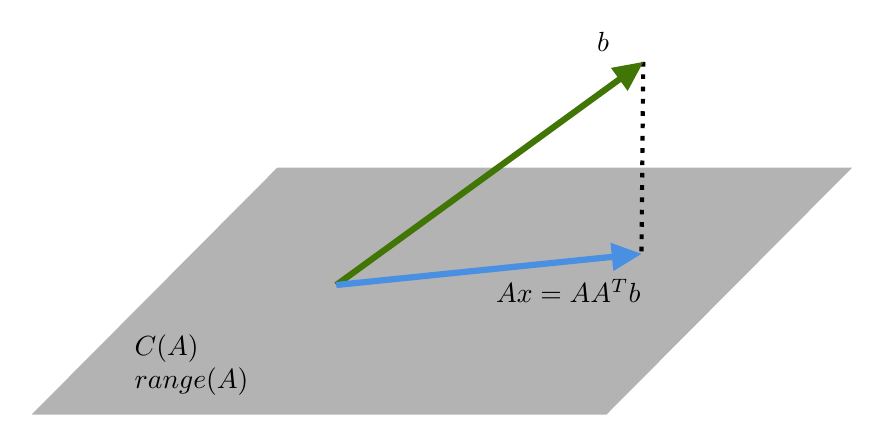
\begin{tikzpicture}[x=0.75pt,y=0.75pt,yscale=-1,xscale=1]
%uncomment if require: \path (0,300); %set diagram left start at 0, and has height of 300

%Shape: Parallelogram [id:dp5765772576295551] 
\draw  [color={rgb, 255:red, 255; green, 255; blue, 255 }  ,draw opacity=1 ][fill={rgb, 255:red, 179; green, 179; blue, 179 }  ,fill opacity=1 ] (203.26,170) -- (481.86,170) -- (362.46,290) -- (83.86,290) -- cycle ;
%Straight Lines [id:da4794253301098559] 
\draw [color={rgb, 255:red, 0; green, 0; blue, 0 }  ,draw opacity=1 ][line width=1.5]  [dash pattern={on 1.69pt off 2.76pt}]  (379.96,119.55) -- (379.07,212) ;
%Straight Lines [id:da5251055282063475] 
\draw [color={rgb, 255:red, 65; green, 117; blue, 5 }  ,draw opacity=1 ][line width=2.25]    (232.07,227) -- (375.92,122.49) ;
\draw [shift={(379.96,119.55)}, rotate = 504] [fill={rgb, 255:red, 65; green, 117; blue, 5 }  ,fill opacity=1 ][line width=0.08]  [draw opacity=0] (14.29,-6.86) -- (0,0) -- (14.29,6.86) -- cycle    ;
%Straight Lines [id:da14492521891839827] 
\draw [color={rgb, 255:red, 74; green, 144; blue, 226 }  ,draw opacity=1 ][line width=2.25]    (232.07,227) -- (374.09,212.51) ;
\draw [shift={(379.07,212)}, rotate = 534.1700000000001] [fill={rgb, 255:red, 74; green, 144; blue, 226 }  ,fill opacity=1 ][line width=0.08]  [draw opacity=0] (14.29,-6.86) -- (0,0) -- (14.29,6.86) -- cycle    ;

% Text Node
\draw (126.72,248.11) node [anchor=north west][inner sep=0.75pt]    {$ \begin{array}{l}
C( A)\\
\operatorname{range}( A)
\end{array}$};
% Text Node
\draw (356.21,103.52) node [anchor=north west][inner sep=0.75pt]    {$b$};
% Text Node
\draw (307.57,222.9) node [anchor=north west][inner sep=0.75pt]    {$Ax=AA^{T} b$};


\end{tikzpicture}

\begin{problem}
    假设矩阵 $ A \in \mathbb{R}^{m \times n} $ \textbf{具有标准正交列},求投影$b$在$C(A)$上的投影。
\end{problem}

即向量 $ A x $ 与$b$有最短距离

$$
\min _{x}\|A x-b\|_{2}^{2}
$$

$$ \begin{aligned} f(x) &=\|A x-b\|_{2}^{2}
    \\ & =(A x-b)^{T}(A x-b)=x^{T} A^{T} A x-2 x^{T} A^{T} b+b^{T} b \\ &=x^{T} x-2 x^{T} A^{T} b+b^{T} b\left(\because A^{T} A=I\right) \end{aligned} $$

$$ \nabla f(x)=2 x-2 A^{T} b=0 \Rightarrow x=A^{T} b $$

$ A A^{T} b $ 称为向量 $ \mathrm{b} \in \mathbb{R}^{m} $ 在 $ \operatorname{range} (A)$上的正交投影。

\begin{theorem}
    $$ A x=A A^{T} b \in \operatorname{range}(A) $$

    且是$b$在$C(A)$上的投影。
\end{theorem}

\begin{proof}
    1.
    $$ A x=A A^{T} b \in \operatorname{range}(A) $$

    2. 可以证明$ \hat{x}=A^{T} b $ 满足 $ \|A \hat{x}-b\|<\|A x-b\| $, 对于所有 $ x \neq \hat{x} $。

    b到range(A)内任意点 $ A x $ 的距离的平方和为:

    $$ \begin{aligned}\|A x-b\|_{2}^{2} &=\|A(x-\hat{x})+A \hat{x}-b\|_{2}^{2} \quad\left(\text {其中 } \hat{x}=A^{T} b\right) \\ &=\|A(x-\hat{x})\|_{2}^{2}+\|A \hat{x}-b\|_{2}^{2}+2(x-\hat{x})^{T} A^{T}(A \hat{x}-b) \\ &=\|A(x-\hat{x})\|_{2}^{2}+\|A \hat{x}-b\|_{2}^{2} \\ &=\|(x-\hat{x})\|_{2}^{2}+\|A \hat{x}-b\|_{2}^{2} \\ & \geq\|A \hat{x}-b\|_{2}^{2} \end{aligned} $$
当且仅当 $ x=\hat{x} $, 等号成立。

第3行成立是因为 $ A^{T}(A \hat{x}-b)=\hat{x}-A^{T} b=0 $ 。
\end{proof}



\tikzset{every picture/.style={line width=0.75pt}} %set default line width to 0.75pt        

\begin{figure}
    \centering
    \caption{Projection of $\boldsymbol{b}$ into the column space of $\boldsymbol{A}$, $A$ is any matrice. Sourced from \cite{Strang1993IntroductionTL}.}
    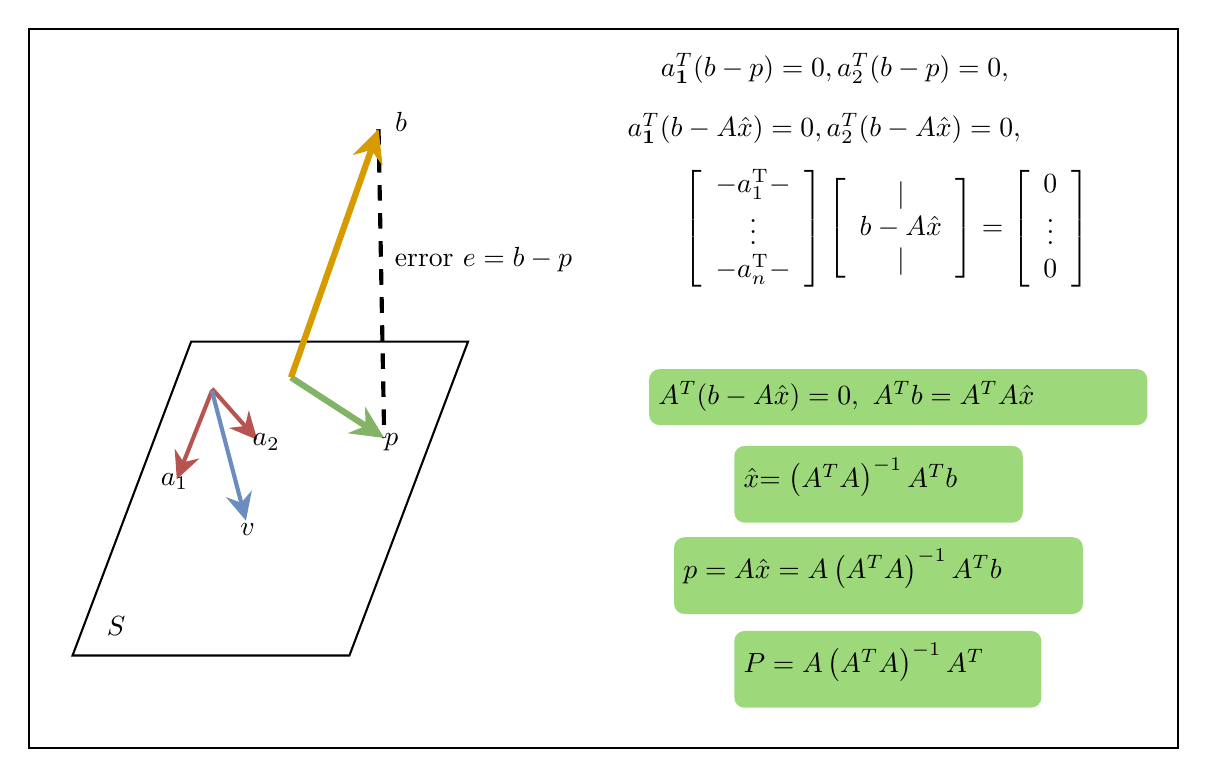
\begin{tikzpicture}[x=0.75pt,y=0.75pt,yscale=-1,xscale=1]
%uncomment if require: \path (0,350); %set diagram left start at 0, and has height of 350

%Straight Lines [id:da0833896477217686] 
\draw [color={rgb, 255:red, 130; green, 179; blue, 102 }  ,draw opacity=1 ][line width=2.25]    (127.38,169.03) -- (168.08,195.47) ;
\draw [shift={(172.28,198.19)}, rotate = 213] [fill={rgb, 255:red, 130; green, 179; blue, 102 }  ,fill opacity=1 ][line width=0.08]  [draw opacity=0] (16.07,-7.72) -- (0,0) -- (16.07,7.72) -- (10.67,0) -- cycle    ;
%Straight Lines [id:da7639150841734914] 
\draw [color={rgb, 255:red, 184; green, 84; blue, 80 }  ,draw opacity=1 ][line width=1.5]    (89.28,175.43) -- (73.82,214.38) ;
\draw [shift={(72.35,218.1)}, rotate = 291.64] [fill={rgb, 255:red, 184; green, 84; blue, 80 }  ,fill opacity=1 ][line width=0.08]  [draw opacity=0] (13.4,-6.43) -- (0,0) -- (13.4,6.44) -- (8.9,0) -- cycle    ;
%Straight Lines [id:da3617082286190523] 
\draw [line width=1.5]  [dash pattern={on 5.63pt off 4.5pt}]  (169.55,49.34) -- (172.28,198.19) ;
%Shape: Parallelogram [id:dp7592583426452624] 
\draw   (79.28,151.73) -- (212.68,151.73) -- (155.51,303) -- (22.11,303) -- cycle ;
%Straight Lines [id:da8449665178781662] 
\draw [color={rgb, 255:red, 184; green, 84; blue, 80 }  ,draw opacity=1 ][line width=1.5]    (89.28,174.43) -- (108.47,196.09) ;
\draw [shift={(111.12,199.08)}, rotate = 228.46] [fill={rgb, 255:red, 184; green, 84; blue, 80 }  ,fill opacity=1 ][line width=0.08]  [draw opacity=0] (13.4,-6.43) -- (0,0) -- (13.4,6.44) -- (8.9,0) -- cycle    ;
%Straight Lines [id:da21760172692551993] 
\draw [color={rgb, 255:red, 106; green, 140; blue, 190 }  ,draw opacity=1 ][line width=1.5]    (89.28,175.43) -- (104.64,234.14) ;
\draw [shift={(105.66,238.01)}, rotate = 255.32999999999998] [fill={rgb, 255:red, 106; green, 140; blue, 190 }  ,fill opacity=1 ][line width=0.08]  [draw opacity=0] (13.4,-6.43) -- (0,0) -- (13.4,6.44) -- (8.9,0) -- cycle    ;
%Straight Lines [id:da9743594112783229] 
\draw [color={rgb, 255:red, 215; green, 155; blue, 0 }  ,draw opacity=1 ][line width=2.25]    (127.38,169.03) -- (167.89,54.06) ;
\draw [shift={(169.55,49.34)}, rotate = 469.41] [fill={rgb, 255:red, 215; green, 155; blue, 0 }  ,fill opacity=1 ][line width=0.08]  [draw opacity=0] (16.07,-7.72) -- (0,0) -- (16.07,7.72) -- (10.67,0) -- cycle    ;
%Shape: Rectangle [id:dp3830905409317218] 
\draw   (1,1) -- (554.64,1) -- (554.64,347.62) -- (1,347.62) -- cycle ;

% Text Node
\draw (175.98,39.87) node [anchor=north west][inner sep=0.75pt]    {$\boldsymbol{b}$};
% Text Node
\draw (170.85,194.49) node [anchor=north west][inner sep=0.75pt]    {$\boldsymbol{p}$};
% Text Node
\draw (107.38,194.77) node [anchor=north west][inner sep=0.75pt]    {$\boldsymbol{a}_{2}$};
% Text Node
\draw (175.92,104.86) node [anchor=north west][inner sep=0.75pt]   [align=left] {error $\displaystyle \boldsymbol{e} =\boldsymbol{b-p}$};
% Text Node
\draw (63.21,213.92) node [anchor=north west][inner sep=0.75pt]    {$\boldsymbol{a}_{1}$};
% Text Node
\draw (101.48,237.88) node [anchor=north west][inner sep=0.75pt]    {$\boldsymbol{v}$};
% Text Node
\draw (37.18,282.9) node [anchor=north west][inner sep=0.75pt]    {$\boldsymbol{S}$};
% Text Node
\draw (288.11,40.4) node [anchor=north west][inner sep=0.75pt]    {$\boldsymbol{a}_{\mathbf{1}}^{T} (\boldsymbol{b} -\boldsymbol{A}\hat{\boldsymbol{x}} )=0,\boldsymbol{a}_{2}^{T} (\boldsymbol{b} -\boldsymbol{A}\hat{\boldsymbol{x}} )=0,\dotsc $};
% Text Node
\draw (304.11,11.4) node [anchor=north west][inner sep=0.75pt]    {$\boldsymbol{a}_{\mathbf{1}}^{T} (\boldsymbol{b} -\boldsymbol{p} )=0,\boldsymbol{a}_{2}^{T} (\boldsymbol{b} -\boldsymbol{p} )=0,\dotsc $};
% Text Node
\draw (314.93,67.4) node [anchor=north west][inner sep=0.75pt]    {$\left[\begin{array}{ c }
-\boldsymbol{a}_{1}^{\mathrm{T}} -\\
\vdots \\
-\boldsymbol{a}_{n}^{\mathrm{T}} -
\end{array}\right]\left[\begin{array}{ c }
\mid \\
\boldsymbol{b} -\boldsymbol{A\hat{\boldsymbol{x}}}\\
\mid 
\end{array}\right] =\left[\begin{array}{ c }
0\\
\vdots \\
0
\end{array}\right]$};
% Text Node
\draw  [color={rgb, 255:red, 0; green, 0; blue, 0 }  ,draw opacity=0 ][fill={rgb, 255:red, 157; green, 217; blue, 123 }  ,fill opacity=1 ]  (299.93,170) .. controls (299.93,167.24) and (302.17,165) .. (304.93,165) -- (534.93,165) .. controls (537.7,165) and (539.93,167.24) .. (539.93,170) -- (539.93,187) .. controls (539.93,189.76) and (537.7,192) .. (534.93,192) -- (304.93,192) .. controls (302.17,192) and (299.93,189.76) .. (299.93,187) -- cycle  ;
\draw (302.93,169.4) node [anchor=north west][inner sep=0.75pt]    {$\boldsymbol{A^{T} (b-A\hat{x} )} =0,\ \boldsymbol{A^{T} b=A^{T} A\hat{x}}$};
% Text Node
\draw  [color={rgb, 255:red, 0; green, 0; blue, 0 }  ,draw opacity=0 ][fill={rgb, 255:red, 157; green, 217; blue, 123 }  ,fill opacity=1 ]  (340.93,207) .. controls (340.93,204.24) and (343.17,202) .. (345.93,202) -- (474.93,202) .. controls (477.7,202) and (479.93,204.24) .. (479.93,207) -- (479.93,234) .. controls (479.93,236.76) and (477.7,239) .. (474.93,239) -- (345.93,239) .. controls (343.17,239) and (340.93,236.76) .. (340.93,234) -- cycle  ;
\draw (343.93,206.4) node [anchor=north west][inner sep=0.75pt]    {$\hat{\boldsymbol{x}}\boldsymbol{=\left( A^{T} A\right)^{-1} A^{T} b}$};
% Text Node
\draw  [color={rgb, 255:red, 157; green, 217; blue, 123 }  ,draw opacity=0 ][fill={rgb, 255:red, 157; green, 217; blue, 123 }  ,fill opacity=1 ]  (311.93,251) .. controls (311.93,248.24) and (314.17,246) .. (316.93,246) -- (503.93,246) .. controls (506.7,246) and (508.93,248.24) .. (508.93,251) -- (508.93,278) .. controls (508.93,280.76) and (506.7,283) .. (503.93,283) -- (316.93,283) .. controls (314.17,283) and (311.93,280.76) .. (311.93,278) -- cycle  ;
\draw (314.93,250.4) node [anchor=north west][inner sep=0.75pt]    {$\boldsymbol{p=A\hat{x} =A\left( A^{T} A\right)^{-1} A^{T} b}$};
% Text Node
\draw  [color={rgb, 255:red, 0; green, 0; blue, 0 }  ,draw opacity=0 ][fill={rgb, 255:red, 157; green, 217; blue, 123 }  ,fill opacity=1 ]  (340.93,296.15) .. controls (340.93,293.38) and (343.17,291.15) .. (345.93,291.15) -- (483.93,291.15) .. controls (486.7,291.15) and (488.93,293.38) .. (488.93,296.15) -- (488.93,323.15) .. controls (488.93,325.91) and (486.7,328.15) .. (483.93,328.15) -- (345.93,328.15) .. controls (343.17,328.15) and (340.93,325.91) .. (340.93,323.15) -- cycle  ;
\draw (343.93,295.55) node [anchor=north west][inner sep=0.75pt]    {$\boldsymbol{P=A\left( A^{T} A\right)^{-1} A^{T}}$};


\end{tikzpicture}
\end{figure}

\chapter{QR Factorization}

\begin{definition}[Lower Triangular Matrices]
    矩阵 $ \mathrm{A} \in \mathbb{R}^{n \times n} $ 为下三角(Lower Triangular)矩阵, $ A_{i j}=0, j>i $ 。

    $$ A=\left[\begin{array}{ccccc}A_{11} & 0 & \cdots & 0 & 0 \\ A_{21} & A_{22} & \cdots & 0 & 0 \\ \vdots & \vdots & \ddots & \vdots & \vdots \\ A_{n-1,1} & A_{n-1,2} & \cdots & A_{n-1, n-1} & 0 \\ A_{n 1} & A_{n 2} & \cdots & A_{n, n-1} & A_{n n}\end{array}\right] $$
\end{definition}

\begin{definition}[Upper Triangular Matrices]
    $ A^{T} $ 为\term{上三角(Upper Triangular)矩阵}。

    $$ A=\left[\begin{array}{ccccc}A_{11} & A_{12} & \cdots & A_{1, n-1} & A_{1, n} \\ 0 & A_{22} & \cdots & A_{2, n-1} & A_{2, n} \\ \vdots & \vdots & \ddots & \vdots & \vdots \\ 0 & 0 & \cdots & A_{n-1, n-1} & A_{n-1, n} \\ 0 & 0 & \cdots & 0 & A_{n n}\end{array}\right] $$
\end{definition}

\begin{definition}[单位上三角矩阵,单位下三角矩阵]
    对角元素 $ a_{i i} $ 都等于 1的上(下)三角矩阵。
\end{definition}

\section{高斯消元法}

\begin{problem}
    当 $ A $ 是具有非零对角元素的下三角矩阵时,解 $ A x=b $ 。
\end{problem}

使用前向回代(Forward Substitution)算法求解。

时间复杂度: $ 1+3+5+\ldots+(2 \mathrm{n}-1)=\mathrm{n}^{2} $ flops

\begin{algorithm}[htbp]
    \caption{Forward Substitution}
    $ x_{1}=b_{1} / A_{11} $\;
$ x_{2}=\left(b_{2}-A_{21} x_{1}\right) / A_{22} $\;
$  x_{3} =\left(b_{3}-A_{31} x_{1}-A_{32} x_{2}\right) / A_{33} $ \;
    $\vdots$  \;
    $x_{n} =\left(b_{n}-A_{n 1} x_{1}-A_{n 2} x_{2}-\cdots-A_{n, n-1} x_{n-1}\right) / A_{n n} $\;
\end{algorithm}

\begin{problem}
    当A是具有非零对角元素的上三角矩阵, 解 $ \mathrm{A} x=\mathrm{b} $ 。
\end{problem}

\begin{algorithm}[htbp]
    \caption{Backward Substitution}

    $ x_{n}=b_{n} / A_{n n} $\;
    $ x_{n-1}=\left(b_{n-1}-A_{n-1, n} x_{n}\right) / A_{n-1, n-1} $ \;
    $ x_{n-2}=\left(b_{n-2}-A_{n-2, n-1} x_{n-1}-A_{n-2, n} x_{n}\right) / A_{n-2, n-2} $\;
    $\cdots$\;
    $ x_{1}=\left(b_{1}-A_{12} x_{2}-A_{13} x_{3}-\cdots-A_{1 n} x_{n}\right) / A_{11} $\;
\end{algorithm}

使用后向回代(Back Substitution)算法来求解.

时间复杂度: $ 1+3+\ldots+2 \mathrm{n}-1=\mathrm{n}^{2} $ flops
\chapter{LU分解}

\section{Solving Linear Equation Systems}

\subsection{Linear Equation Systems}
\begin{example}
    \begin{equation}
         A\boldsymbol{x} =\boldsymbol{b} \Leftrightarrow { \left\{\begin{matrix}
        x & + & 2y & + & 3z & = & 6\\
        2x & + & 5y & + & 2z & = & 4\\
        6x & - & 3y & + & z & = & 2
        \end{matrix}\right. }
         \end{equation}
\end{example}

见Row Picture,Column Picture的概念。

\subsection{Elimination}

\begin{example}[Elimination]
    Before

        \begin{equation} \left\{\begin{matrix}
        x & - & 2y & = & 1\\
        3x & + & 2y & = & 11
        \end{matrix}\right. \end{equation}
        
        
   
    After
    
    \begin{equation} \left\{\begin{matrix}
        x & - & 2y & = & 1\\
         &  & 8y & = & 8
        \end{matrix}\right. \end{equation}
    

\end{example}

\begin{definition}[Pivot]
    The first nonzero in the row that does elimination. \textbf{Zero is not allowed as a pivot.}
\end{definition}

\begin{definition}[Multiplier]
    (Entry to eliminate) divided by (pivot)
\end{definition}

消元法通过elimination matrices $E$进行消元操作,使得主对角线以下的元素为0. Multiply the $ j^{\text {th }} $ equation by $ \ell_{i j} $ and subtract from the $ i^{\text {th }} $ equation. (This eliminates $ x_{j} $ from equation $ i $.) We need a lot of these simple matrices $ E_{i j} $, one for every nonzero to be eliminated below the main diagonal.

\begin{definition}[Elementary matrix, Elimination matrix]
    The elementary matrix or elimination matrix $ E_{i j} $ has the extra nonzero entry $ -\ell $ in the $ i, j $ position. Then $ E_{i j} $ subtracts a multiple $ \ell $ of row $ j $ from row $ i $.
\end{definition}

\begin{theorem}
    消元法的本质是

    \begin{equation}Ax= b \Rightarrow EAx = Eb\end{equation}
\end{theorem}

\begin{definition}[Permutation matrices $P$]
    $  P_{i j} $ is the identity matrix with rows $ i $ and $ j $ reversed. When this \term{permutation matrix} $ P_{i j} $ multiplies a matrix, it exchanges rows $ i $ and $ j $.
\end{definition}

\begin{definition}[Augmented matrix]
    \begin{equation} \left[\begin{matrix}
                A & b
            \end{matrix}\right]\end{equation}
\end{definition}

\subsubsection{Computing $A^{-1}$ by Gauss-Jordan Elimination}

\begin{center}
    Multiply $ \left[\begin{matrix}
                A & I
            \end{matrix}\right]$ by $ A^{-1}$ to get $ \left[\begin{matrix}
                I & A^{-1}
            \end{matrix}\right]$
\end{center}

\begin{remark}
    The inverse exists if and only if elimination produces $n$ pivots. Row exchanges are allowed. Elimination solves $Ax = b$ without explicitly using the matrix $A^{-1}$.
\end{remark}

\begin{remark}
    (Important) Suppose there is a nonzero vector $ x $ such that $ A x=0 . $ Then $ A $ cannot have an inverse. No matrix can bring $ \mathbf{0} $ back to $ \boldsymbol{x} $.

If $ A $ is invertible, then $ A x=0 $ can only have the \textbf{zero solution} $ x=A^{-1} 0=0 $.
\end{remark}


\begin{example}
    \begin{equation} \begin{aligned}\left[\begin{array}{llll}K & e_{1} & e_{2} & e_{3}\end{array}\right] & =\left[\begin{array}{rrrrrr}\mathbf{2} & -\mathbf{1} & \mathbf{0} & 1 & 0 & 0 \\ -\mathbf{1} & \mathbf{2} & -\mathbf{1} & 0 & 1 & 0 \\ \mathbf{0} & -\mathbf{1} & \mathbf{2} & 0 & 0 & 1\end{array}\right] \quad \text { Start Gauss-Jordan on } K                                                  \\ & \rightarrow\left[\begin{array}{rrrrrr}2 & -1 & 0 & 1 & 0 & 0 \\ \mathbf{0} & \frac{3}{2} & -\mathbf{1} & \frac{1}{2} & \mathbf{1} & \mathbf{0} \\ 0 & -1 & 2 & 0 & 0 & 1\end{array}\right] \quad\left(\frac{\mathbf{1}}{\mathbf{2}} \text { row } 1+\text { row 2 }\right) \\ & \rightarrow\left[\begin{array}{rrrrrr}2 & -1 & 0 & 1 & 0 & 0 \\ 0 & \frac{3}{2} & -1 & \frac{1}{2} & 1 & 0 \\ \mathbf{0} & \mathbf{0} & \frac{4}{3} & \frac{1}{3} & \frac{2}{3} & \mathbf{1}\end{array}\right] \quad \left(\frac{\mathbf{2}}{3} \text { row 2 + row 3}\right)\\
               \left(\begin{array}{c}\text { Zero above } \\ \text { third pivot }\end{array}\right) & \rightarrow\left[\begin{array}{rrrrrr}2 & -1 & 0 & 1 & 0 & 0 \\ 0 & \frac{3}{2} & 0 & \frac{3}{4} & \frac{3}{2} & \frac{3}{4} \\ 0 & 0 & \frac{4}{3} & \frac{1}{3} & \frac{2}{3} & 1\end{array}\right] \quad\left(\frac{3}{4} \text{ row } \mathbf{3}+ \text{ row } \mathbf{2}\right) \\
               \left(\begin{array}{l}\text { Zero above } \\ \text { second pivot }\end{array}\right) & \rightarrow\left[\begin{array}{cccccc}2 & 0 & 0 & \frac{3}{2} & 1 & \frac{1}{2} \\ 0 & \frac{3}{2} & 0 & \frac{3}{4} & \frac{3}{2} & \frac{3}{4} \\ 0 & 0 & \frac{4}{3} & \frac{1}{3} & \frac{2}{3} & 1\end{array}\right] \quad\left(\frac{2}{3} \text{ row } 2+ \text{ row }1 \right)
        \end{aligned} \end{equation}


    然后将它变成Reduced echelon form $R$.

   
    \begin{equation} \begin{matrix}
                (\text{divided by }2)                      \\
                \left(\text{divided by }\dfrac{3}{2}\right) \\
                \left(\text{divided by }\dfrac{4}{3}\right)
            \end{matrix}\left[\begin{matrix}
                    1 & 0 & 0 & \dfrac{3}{4} & \dfrac{1}{2} & \dfrac{1}{4} \\
                    0 & 1 & 0 & \dfrac{1}{2} & 1           & \dfrac{1}{2} \\
                    0 & 0 & 1 & \dfrac{1}{4} & \dfrac{1}{2} & \dfrac{3}{4}
                \end{matrix}\right] =\left[\begin{matrix}
                    I & x_{1} & x_{2} & x_{3}
                \end{matrix}\right] =\ \left[\begin{matrix}
                    I & K^{-1}
                \end{matrix}\right]\end{equation}
    


    \begin{enumerate}
        \item $ K $ is symmetric across its main diagonal. Then $ K^{-1} $ is also symmetric.
        \item $ K $ is tridiagonal (only three nonzero diagonals). But $ K^{-1} $ is a dense matrix with no zeros. That is another reason we don't often compute inverse matrices. The inverse of a band matrix is generally a dense matrix.
        \item The product of pivots is $ 2\left(\frac{3}{2}\right)\left(\frac{4}{3}\right)=4 $. This number 4 is the determinant of $ K $. $ K^{-1} $ involves division by the determinant of $ K $.
        \begin{equation} K^{-1}=\frac{1}{4}\left[\begin{array}{lll}3 & 2 & 1 \\ 2 & 4 & 2 \\ 1 & 2 & 3\end{array}\right] \end{equation}
    \end{enumerate}


    This is why an \textbf{invertible matrix} cannot have a \textbf{zero determinant}: we need to \textbf{divide}.

\end{example}

\section{LU分解}

$ \left(E_{32} E_{31} E_{21}\right) A=U \quad $ becomes $ \quad A=\left(E_{21}^{-1} E_{31}^{-1} E_{32}^{-1}\right) U \quad $ which is $ \quad A=L U $

\begin{theorem}
    When a row of $A$ starts with zeros, so does that row of $L$.

    When a column of $A$ starts with zeros, so does that column of $U$.
\end{theorem}

\begin{example}[The key reason why $ A $ equals $ L U$]
    Ask yourself about the pivot rows that are subtracted from lower rows. Are they the original rows of $ A ? $ No, elimination probably changed them.

    Are they rows of $ U ? $ Yes, the pivot rows never change again.

    When computing the third row of $ U $, we subtract multiples of earlier rows of $ U $ (not rows of $ A ! $ ):
    \begin{equation} \text{Row 3 of }  U=(\text{Row 3 of }  A)-\ell_{31}(
        \text{Row 1 of } U)-\ell_{32}(\text{Row 2 of }  of  U) \end{equation}

    Rewrite this equation to see that the row $ \left[\begin{array}{lll}\ell_{31} & \ell_{32} & 1\end{array}\right] $ is multiplying the matrix $ U $ :

    \begin{equation} (\text{Row 3 of } A)=\ell_{31}(\text{Row 1 of }  U)+\ell_{32}(\text{Row 2 of } U)+1(\text{Row 3 of }  U) \end{equation}

    This is exactly row 3 of $ A=L U . $

    That row of $
        L $ holds $ \ell_{31}, \ell_{32}, 1 . $ All rows look like this, whatever the size of $ A $. With no row exchanges, we have $ A=L U $.
\end{example}

\begin{definition}[$A$的LU分解]
    \begin{equation} A=\left(\begin{array}{ccccc}a_{11} & \cdots & a_{1 k} & \cdots & a_{1 n} \\ \vdots & \ddots & \vdots & & \vdots \\ a_{k 1} & \cdots & a_{k k} & \cdots & a_{k n} \\ \vdots & & \vdots & \ddots & \vdots \\ a_{n 1} & \cdots & a_{n k} & \cdots & a_{n n}\end{array}\right) =LU \end{equation}

    where $ L=\left(\begin{array}{cccc}1 & 0 & \cdots & 0 \\ l_{21} & 1 & \ddots & 0 \\ \vdots & \vdots & \ddots & 0 \\ l_{n 1} & l_{n 2} & \cdots & 1\end{array}\right) , U=\left(\begin{array}{cccc}u_{11} & u_{12} & \cdots & u_{1 n} \\ 0 & u_{22} & \cdots & u_{2 n} \\ \vdots & 0 & \ddots & \vdots \\ 0 & 0 & 0 & u_{n n}\end{array}\right) $
\end{definition}

所以
\begin{equation}
    \begin{aligned}
        A & =\left(\begin{array}{ccccc}a_{11} & \cdots & a_{1 r} & \cdots & a_{1 n} \\ \vdots & \ddots & \vdots & & \vdots \\ a_{r 1} & \cdots & a_{r r} & \cdots & a_{r n} \\ \vdots & & \vdots & \ddots & \vdots \\ a_{n 1} & \cdots & a_{n r} & \cdots & a_{n n}\end{array}\right)                                               \\
          & =\left(\begin{array}{ccccc}1 & 0 & 0 & \cdots & 0 \\ \vdots & \ddots & 0 & \ddots & 0 \\ l_{r 1} & \cdots & 1 & \ddots & \vdots \\ \vdots & & \vdots & \ddots & 0 \\ l_{n 1} & \cdots & l_{n r} & \cdots & 1\end{array}\right) \cdot \left(\begin{array}{cccc}u_{11} & u_{12} & \cdots & u_{1 n} \\ 0 & u_{22} & \cdots & u_{2 n} \\ \vdots & 0 & \ddots & \vdots \\ 0 & 0 & 0 & u_{n n}\end{array}\right)
    \end{aligned}
\end{equation}

\subsection{$A = LDU$}

$A=LU$是不对称的。但是可以改写为对称形式。

Split $ U $ into $ \left[\begin{array}{cccc}d_{1} & & & \\ & d_{2} & & \\ & & \ddots & \\ & & & d_{n}\end{array}\right]\left[\begin{array}{cccc}1 & u_{12} / d_{1} & u_{13} / d_{1} & \cdot \\ & 1 & u_{23} / d_{2} & \cdot \\ & & \ddots & \vdots \\ & & & 1\end{array}\right] $.

\begin{example}
    
    \begin{equation}(A= LU) \left[\begin{array}{ll}1 & 0 \\ 3 & 1\end{array}\right]\left[\begin{array}{ll}2 & 8 \\ 0 & 5\end{array}\right] \end{equation} 
    
    splits further into
    
    \begin{equation}(A= LDU) \left[\begin{array}{ll}1 & 0 \\ 3 & 1\end{array}\right]\left[\begin{array}{ll}2 & \\ & 5\end{array}\right]\left[\begin{array}{ll}1 & 4 \\ 0 & 1\end{array}\right] \end{equation}.
    
\end{example}

\begin{theorem}
    当$A$是对称矩阵的时候,且消元的时候不需要行交换:

    \begin{equation}S = LDL^T\end{equation}
\end{theorem}


\begin{example}
    \begin{equation} \left[\begin{array}{ll}1 & 2 \\ 2 & 7\end{array}\right]=\left[\begin{array}{ll}\mathbf{1} & 0 \\ \mathbf{2} & \mathbf{1}\end{array}\right] \quad\left[\begin{array}{ll}1 & 0 \\ 0 & 3\end{array}\right] \quad\left[\begin{array}{ll}\mathbf{1} & \mathbf{2} \\ 0 & \mathbf{1}\end{array}\right] \end{equation}
\end{example}


\subsection{$L$、$U$矩阵的性质}

回顾矩阵乘法的定义

\begin{definition}[矩阵乘法]
    设矩阵 $ A \in \mathbb{R}^{m \times p}, B \in \mathbb{R}^{p \times n} $,那么矩阵$A$与$B$的乘积, 记 作C $ =A B $ ,  则矩阵 $ C \in \mathbb{R}^{m \times n} $ 的第 $i$行第 $ j $ 列元素 $ C_{i j} $


    \begin{equation}
{C}_{i j}=\sum_{k=1}^{p} A_{i k} B_{k j}
\end{equation}
\end{definition}

对于$L$、$U$有

\begin{theorem}
    $ A $ 的第一行元素 $ a_{1 j} $ 为
    \begin{equation}
        a_{1 j}=u_{1 j}, j=1, \cdots, n
    \end{equation}
\end{theorem}

\begin{corollary}
    $ U $ 的第一行元素 $ u_{1 j} $ 为
    \begin{equation}
        u_{1 j}=a_{1 j}, j=1, \cdots, n
    \end{equation}
\end{corollary}

\begin{proof}
    \begin{equation} \begin{aligned}A & =\left(\begin{array}{ c c c c c }
                \boldsymbol{\textcolor[rgb]{0.72,0.33,0.31}{a_{11}}} & \boldsymbol{\textcolor[rgb]{0.72,0.33,0.31}{\cdots }} & \boldsymbol{\textcolor[rgb]{0.72,0.33,0.31}{a_{1r}}} & \boldsymbol{\textcolor[rgb]{0.72,0.33,0.31}{\cdots }} & \boldsymbol{\textcolor[rgb]{0.72,0.33,0.31}{a_{1n}}} \\
                \vdots                                               & \ddots                                                & \vdots                                               &                                                       & \vdots                                               \\
                a_{r1}                                               & \cdots                                                & a_{rr}                                               & \cdots                                                & a_{rn}                                               \\
                \vdots                                               &                                                       & \vdots                                               & \ddots                                                & \vdots                                               \\
                a_{n1}                                               & \cdots                                                & a_{nr}                                               & \cdots                                                & a_{nn}
            \end{array}\right)
               \\ &=\left(\begin{array}{ c c c c c }
                \boldsymbol{\textcolor[rgb]{0.72,0.33,0.31}{1}} & 0      & 0      & \cdots & 0      \\
                \vdots                                          & \ddots & 0      & \ddots & 0      \\
                l_{r1}                                          & \cdots & 1      & \cdots & \vdots \\
                \vdots                                          & \ddots & \vdots & \ddots & 0      \\
                l_{n1}                                          & \cdots & l_{nr} & \cdots & 1
            \end{array}\right) \cdot \left(\begin{array}{ c c c c c }
                \boldsymbol{\textcolor[rgb]{0.72,0.33,0.31}{u_{11}}} & \boldsymbol{\textcolor[rgb]{0.72,0.33,0.31}{\cdots }} & \boldsymbol{\textcolor[rgb]{0.72,0.33,0.31}{u_{1r}}} & \boldsymbol{\textcolor[rgb]{0.72,0.33,0.31}{\cdots }} & \boldsymbol{\textcolor[rgb]{0.72,0.33,0.31}{u_{1n}}} \\
                0                                                    & \ddots                                                & \vdots                                               & \ddots                                                & \vdots                                               \\
                0                                                    & 0                                                     & u_{rr}                                               & \cdots                                                & u_{rn}                                               \\
                \vdots                                               & \ddots                                                & 0                                                    & \ddots                                                & \vdots                                               \\
                0                                                    & \cdots                                                & 0                                                    & 0                                                     & u_{nn}
            \end{array}\right)\end{aligned}\end{equation}
\end{proof}

\begin{corollary}
    $ L $ 的第一列元素 $ l_{i1} $ 为

    \begin{equation} l_{i 1}=\frac{a_{i 1}}{u_{11}} , i=2,3, \cdots, n \end{equation}
\end{corollary}

\begin{proof}
    \begin{equation} \begin{aligned} A & =\left(\begin{array}{ c c c c c }
                \boldsymbol{\textcolor[rgb]{0.72,0.33,0.31}{a_{11}}}  & \cdots & a_{1r} & \cdots & a_{1n} \\
                \boldsymbol{\textcolor[rgb]{0.72,0.33,0.31}{\vdots }} & \ddots & \vdots &        & \vdots \\
                \boldsymbol{\textcolor[rgb]{0.72,0.33,0.31}{a_{r1}}}  & \cdots & a_{rr} & \cdots & a_{rn} \\
                \boldsymbol{\textcolor[rgb]{0.72,0.33,0.31}{\vdots }} &        & \vdots & \ddots & \vdots \\
                \boldsymbol{\textcolor[rgb]{0.72,0.33,0.31}{a_{n1}}}  & \cdots & a_{nr} & \cdots & a_{nn}
            \end{array}\right)                                               \\
                  & =\left(\begin{array}{ c c c c c }
                \boldsymbol{\textcolor[rgb]{0.72,0.33,0.31}{1}}       & 0      & 0      & \cdots & 0      \\
                \boldsymbol{\textcolor[rgb]{0.72,0.33,0.31}{\vdots }} & \ddots & 0      & \ddots & 0      \\
                \boldsymbol{\textcolor[rgb]{0.72,0.33,0.31}{l_{r1}}}  & \cdots & 1      & \ddots & \vdots \\
                \boldsymbol{\textcolor[rgb]{0.72,0.33,0.31}{\vdots }} &        & \vdots & \ddots & 0      \\
                \boldsymbol{\textcolor[rgb]{0.72,0.33,0.31}{l_{n1}}}  & \cdots & l_{nr} & \cdots & 1
            \end{array}\right) \cdot \left(\begin{array}{ c c c c c }
                \boldsymbol{\textcolor[rgb]{0.72,0.33,0.31}{u_{11}}} & \cdots & u_{1r} & \cdots & u_{1n} \\
                0                                                    & \ddots & \vdots & \ddots & \vdots \\
                0                                                    & 0      & u_{rr} & \cdots & u_{rn} \\
                \vdots                                               & \ddots & 0      & \ddots & \vdots \\
                0                                                    & \cdots & 0      & 0      & u_{nn}
            \end{array}\right)
        \end{aligned}\end{equation}
\end{proof}

\begin{theorem}
    $ A $ 的第 $ r $ 行主对角线以右元素 $ a_{r j}(j=1, \cdots, n, j \ge r) $ 为

    \begin{equation}a_{r j}=\sum_{k=1}^{r} l_{r k} u_{k j}, r=1,2, \cdots, n,j=r, \cdots, n \end{equation}
\end{theorem}

\begin{proof}
    \begin{equation}
        \begin{aligned}
            A & =\left(\begin{array}{ c c c c c c c }
            a_{11} & \cdots  & a_{1r} & \cdots  & a_{1j} & \cdots  & a_{1n}\\
            \vdots  & \ddots  & \vdots  &  & \vdots  &  & \vdots \\
            a_{r1} & \cdots  & a_{rr} & \cdots  & \boldsymbol{\textcolor[rgb]{0.72,0.33,0.31}{a}\textcolor[rgb]{0.72,0.33,0.31}{_{rj}}} & \cdots  & a_{rn}\\
            \vdots  &  & \vdots  & \ddots  & \vdots  & \ddots  & \vdots \\
            a_{n1} & \cdots  & a_{nr} & \cdots  &  & \cdots  & a_{nn}
            \end{array}\right)\\
             & =\left(\begin{array}{ c c c c c c }
            1 & 0 & 0 & 0 & \cdots  & 0\\
            \vdots  & \ddots  & 0 & 0 & \ddots  & \vdots \\
            \boldsymbol{\textcolor[rgb]{0.72,0.33,0.31}{l}\textcolor[rgb]{0.72,0.33,0.31}{_{r1}}} & \boldsymbol{\textcolor[rgb]{0.72,0.33,0.31}{\cdots }} & \boldsymbol{\textcolor[rgb]{0.72,0.33,0.31}{1}} & 0 & \cdots  & 0\\
            \vdots  & \ddots  & \vdots  & 1 & \ddots  & \vdots \\
            l_{n1} & \cdots  & l_{nr} & l_{n,r+1} & \cdots  & 1
            \end{array}\right) \cdot \left(\begin{array}{ c c c c c c c }
            u_{11} & \cdots  & u_{1r} & \cdots  & \boldsymbol{\textcolor[rgb]{0.72,0.33,0.31}{u}\textcolor[rgb]{0.72,0.33,0.31}{_{1j}}} & \cdots  & u_{1n}\\
            0 & \ddots  & \vdots  & \ddots  & \boldsymbol{\textcolor[rgb]{0.72,0.33,0.31}{\vdots }} & \cdots  & \vdots \\
            0 & 0 & u_{rr} & \cdots  & \boldsymbol{\textcolor[rgb]{0.72,0.33,0.31}{u}\textcolor[rgb]{0.72,0.33,0.31}{_{rj}}} & \cdots  & u_{rn}\\
            \vdots  & \ddots  & 0 & \ddots  & u_{r+1,j} & \cdots  & \vdots \\
            0 & \cdots  & 0 & 0 & 0 & \ddots  & u_{nn}
            \end{array}\right)
            \end{aligned}
    \end{equation}

    由于$l_{rj}, j > r$都是0,所以求和只需加和到第$r$项。
\end{proof}

\begin{corollary}
    $U$第 $ r $ 行主对角线以右元素 $ u_{r j} $

    \begin{equation} u_{r j}=a_{r j}-\sum_{k=1}^{r-1} l_{r k} u_{k j}, j = r, \cdots, n \end{equation}
\end{corollary}

\begin{proof}
    \begin{equation}\begin{aligned}
                        & a_{r j}=\sum_{k=1}^{r} l_{r k} u_{k j}, r=1,2, \cdots, n,j=r, \cdots, n                     \\
            \Rightarrow & a_{r j}=\sum_{k=1}^{r - 1} l_{r k} u_{k j} + l_{rr} u_{rj}, r=1,2, \cdots, n,j=r, \cdots, n \\
            \Rightarrow & u_{r j}=a_{r j}-\sum_{k=1}^{r-1} l_{r k} u_{k j}, j = r, \cdots, n
        \end{aligned}\end{equation}
\end{proof}


\begin{corollary}
    $U$的对角线元素$u_{r r}$

    \begin{equation} u_{r r}=a_{r r}-\sum_{k=1}^{r-1} l_{r k} u_{k r} \end{equation}
\end{corollary}


\begin{theorem}
    $ A $ 的第 $ r $ 列元素主对角线以下元素 $ a_{i r}(i=r+1, \cdots, n) $ 为

    \begin{equation}a_{i r}=\sum_{k=1}^{r} l_{i k} u_{k r}, i=r+1, \cdots, n, r=1,2, \cdots, n-1 \end{equation}
\end{theorem}

\begin{proof}
    \begin{equation}
        \begin{aligned}
            A & =\left(\begin{array}{ c c c c c c c }
            a_{11} & \cdots  & a_{1j} & \cdots  & a_{1r} & \cdots  & a_{1n}\\
            \vdots  & \ddots  & \vdots  &  & \vdots  &  & \vdots \\
            a_{r1} & \cdots  & \boldsymbol{\textcolor[rgb]{0.72,0.33,0.31}{a_{rj}}} & \cdots  & a_{rr} & \cdots  & a_{rn}\\
            \vdots  &  & \vdots  &  & \vdots  & \ddots  & \vdots \\
            a_{n1} & \cdots  & a_{nj} & \cdots  & a_{nr} & \cdots  & a_{nn}
            \end{array}\right)\\
             & =\left(\begin{array}{ c c c c c c }
            1 & 0 & 0 & 0 & \cdots  & 0\\
            \vdots  & \ddots  & 0 & 0 & \ddots  & \vdots \\
            \boldsymbol{\textcolor[rgb]{0.72,0.33,0.31}{l}\textcolor[rgb]{0.72,0.33,0.31}{_{r1}}} & \boldsymbol{\textcolor[rgb]{0.72,0.33,0.31}{\cdots }} & \boldsymbol{\textcolor[rgb]{0.72,0.33,0.31}{1}} & 0 & \cdots  & 0\\
            \vdots  & \ddots  & \vdots  & 1 & \ddots  & \vdots \\
            l_{n1} & \cdots  & l_{nr} & l_{n,r+1} & \cdots  & 1
            \end{array}\right) \cdot \left(\begin{array}{ c c c c c c c }
            u_{11} & \cdots  & \boldsymbol{\textcolor[rgb]{0.72,0.33,0.31}{u_{1j}}} & \cdots  & u_{1r} & \cdots  & u_{1n}\\
            0 & \ddots  & \boldsymbol{\textcolor[rgb]{0.72,0.33,0.31}{\vdots }} & \ddots  & \vdots  & \cdots  & \vdots \\
            0 & 0 & \boldsymbol{\textcolor[rgb]{0.72,0.33,0.31}{u_{jj}}} & \cdots  & u_{rr} & \cdots  & u_{rn}\\
            \vdots  & \ddots  & 0 & \ddots  & 0 & \cdots  & \vdots \\
            0 & \cdots  & 0 & 0 & 0 & \ddots  & u_{nn}
            \end{array}\right)
            \end{aligned}
    \end{equation}

    由于$u_{rj}, r > j$都是0,所以求和只需加和到第$r$项。
\end{proof}

\begin{corollary}
    显然, $ r=1 $ 时

    \begin{equation} a_{i 1}=l_{i 1} u_{11} , i=2,3, \cdots, n \end{equation}
\end{corollary}

\begin{corollary}
    $L$第 $ r $ 列主对角线以下元素 $ l_{i r} $

    \begin{equation} l_{i r}=\frac{a_{i r}-\sum_{k=1}^{r-1} l_{i k} u_{k r}}{u_{r r}}, i = r + 1, \cdots, n \end{equation}
\end{corollary}






\subsection{Solving $Ax = b$ Using LU Decomposition and its Complexity}
\label{Ax-eqs-b-LU}

求解 $ A x=b, A $ 为非奇异矩阵,LU算法为求解方程组 $ A x=b $ 的标准解法。

复杂度: $ \frac{2}{3} n^{3}+2 n^{2} \approx \frac{2}{3} n^{3} $ flops

\begin{algorithm}[htbp]
    \caption{Solving $Ax = b$ Using LU Decomposition}
    对矩阵 $ A $ 进行LU分解 $ \left(\frac{2}{3} n^{3} \text{flops} \right) $\;
    回代法: 求解 $ L y=b\left(n^{2}\text{flops} \right) $\;
    回代法: 求解 $ U x=y\left(n^{2}\text{flops} \right) $\;
\end{algorithm}


\subsection{Example of LU Decomposition}

\begin{example}
    对矩阵 $ A $ 进行 $ L U $ 分解
    \begin{equation}
        A=\left[\begin{array}{lll}
                8 & 2 & 9 \\
                4 & 9 & 4 \\
                6 & 7 & 9
            \end{array}\right]
    \end{equation}


    \begin{equation} A=\left[\begin{array}{lll}8 & 2 & 9 \\ 4 & 9 & 4 \\ 6 & 7 & 9\end{array}\right]=\left[\begin{array}{ccc}1 & 0 & 0 \\ l_{21} & 1 & 0 \\ l_{31} & l_{32} & 1\end{array}\right]\left[\begin{array}{ccc}u_{11} & u_{12} & u_{13} \\ 0 & u_{22} & u_{23} \\ 0 & 0 & u_{33}\end{array}\right] \end{equation}

    计算$U$的第一行和 $ L $ 的第一列

    \begin{equation} \left(u_{11}, u_{12}, u_{13}\right)=(8,2,9) , \left(l_{21}, l_{31}\right)=\left(\frac{1}{2}, \frac{3}{4}\right) \end{equation}

    然后计算$U$的第二行和$L$的第二列

    \begin{equation} u_{22}=a_{22}-l_{21} u_{12}=8 ,
        u_{23}=a_{23}-l_{21} u_{13}=-\frac{1}{2} , l_{32}=\frac{a_{32}-l_{31} u_{12}}{u_{22}}=\frac{11}{16} \end{equation}


    最后计算$U$的第三行

    \begin{equation} u_{33}=a_{33}-l_{31}  u_{13}-l_{32} u_{23}=-\frac{83}{32} \end{equation}

\end{example}

\section{Problem of LU Decomposition}


\begin{example}
    \begin{equation} A=\left[\begin{array}{ccc}1 & 0 & 0 \\ 0 & 0 & 2 \\ 0 & 1 & -1\end{array}\right]=\left[\begin{array}{ccc}1 & 0 & 0 \\ l_{21} & 1 & 0 \\ l_{31} & L_{32} & 1\end{array}\right]\left[\begin{array}{ccc}u_{11} & u_{12} & u_{13} \\ 0 & u_{22} & u_{23} \\ 0 & 0 & u_{33}\end{array}\right] \end{equation}

    计算$U$的第一行和$L$的第一列
    \begin{equation}
        \left[\begin{array}{ccc}
                1 & 0 & 0  \\
                0 & 0 & 2  \\
                0 & 1 & -1
            \end{array}\right]=\left[\begin{array}{ccc}
                1 & 0      & 0 \\
                0 & 1      & 0 \\
                0 & l_{32} & 1
            \end{array}\right]\left[\begin{array}{ccc}
                1 & 0      & 0      \\
                0 & u_{22} & u_{23} \\
                0 & 0      & u_{33}
            \end{array}\right]
    \end{equation}

    然后计算$U$的第二行和$L$的第二列
    \begin{equation}
        \begin{array}{l}
            u_{22}=a_{22}-l_{21} u_{12}=0 \\
            u_{23}=a_{23}-l_{21} u_{13}=2
        \end{array} \quad l_{32}=\frac{a_{32}-l_{31} u_{12}}{u_{22}}=\frac{1}{\boldsymbol{0}}
    \end{equation}
    即该矩阵无法 $ {LU} $ 分解!

    通过$PA=LU$分解,可以得到LU分解

    \begin{equation}P=\left[\begin{matrix}
        1 & 0 & 0\\
        0 & 1 & 0\\
        0 & 0 & 1
        \end{matrix}\right] ,L=\left[\begin{matrix}
        1 & 0 & 0\\
        0 & 1 & -1\\
        0 & 0 & 2
        \end{matrix}\right] ,U=\left[\begin{matrix}
        1 & 0 & 0\\
        0 & 0 & 1\\
        0 & 1 & 0
        \end{matrix}\right]\end{equation}
\end{example}

\section{\texorpdfstring{$PA=LU$}{PA=LU}}

\begin{theorem}
    非奇异矩阵 $ {A} \in \mathbb{R}^{n \times n} $ ,则可分解为 $ A=P^{T} L U $

    $ P $ 是一个置换矩阵, $ L $ 为下三角矩阵并且对角线元素全为 $ 1 , U $ 为 上三角矩阵。
\end{theorem}


$PA=LU$分解方法不唯一,随着 $ P $ 的选择不同, $L$、$U$也不同。

\begin{example}[$PA=LU$]

    假设
    \begin{equation} A=\left[\begin{array}{lll}0 & 5 & 5 \\ 2 & 9 & 0 \\ 6 & 8 & 8\end{array}\right], P_{1}=\left[\begin{array}{lll}0 & 0 & 1 \\ 0 & 1 & 0 \\ 1 & 0 & 0\end{array}\right], P_{2}=\left[\begin{array}{lll}0 & 1 & 0 \\ 1 & 0 & 0 \\ 0 & 0 & 1\end{array}\right] \end{equation}

    易知
    \begin{equation}P_{1}^{T}=P_{1}^{-1}=P_{1}, P_{2}^{T}=P_{2}^{-1}=P_{2}\end{equation}

    计算可得
    \begin{equation} P_{1} A=\left[\begin{array}{lll}6 & 8 & 8 \\ 2 & 9 & 0 \\ 0 & 5 & 5\end{array}\right], P_{2} A=\left[\begin{array}{lll}2 & 9 & 0 \\ 0 & 5 & 5 \\ 6 & 8 & 8\end{array}\right] \end{equation}

    LU分解不唯一:

    \begin{equation}
        P_{1} A=\left[\begin{array}{lll}
                6 & 8 & 8 \\
                2 & 9 & 0 \\
                0 & 5 & 5
            \end{array}\right]=\left[\begin{array}{ccc}
                1           & 0             & 0 \\
                \frac{1}{3} & 1             & 0 \\
                0           & \frac{15}{19} & 1
            \end{array}\right]\left[\begin{array}{ccc}
                6 & 8            & 8              \\
                0 & \frac{19}{3} & \frac{-8}{3}   \\
                0 & 0            & \frac{135}{19}
            \end{array}\right]=L_{1} U_{1} \Rightarrow A=P_{1} L_{1} U_{1}
    \end{equation}


    \begin{equation} P_{2} A=\left[\begin{array}{lll}2 & 9 & 0 \\ 0 & 5 & 5 \\ 6 & 8 & 8\end{array}\right]=\left[\begin{array}{ccc}1 & 0 & 0 \\ 0 & 1 & 0 \\ 3 & \frac{-19}{5} & 1\end{array}\right]\left[\begin{array}{ccc}2 & 9 & 2 \\ 0 & 5 & 5 \\ 0 & 0 & 27\end{array}\right]=L_{2} U_{2} \Rightarrow A=P_{2} L_{2} U_{2} \end{equation}

\end{example}


\begin{theorem}
    这个方法等价于对$A$进行行初等变换然后对 $ P A $ 进行分解 $ P A=L U $.
\end{theorem}

\subsubsection{The Complexity of $PA = LU$}

\label{complexity:PA-eqs-LU}

复杂度: $ \frac{2}{3} n^{3} $ flops



\section{舍入误差的影响}

\begin{example}
    \begin{equation} \left[\begin{array}{cc}10^{-5} & 1 \\ 1 & 1\end{array}\right]\left[\begin{array}{l}x_{1} \\ x_{2}\end{array}\right]=\left[\begin{array}{l}1 \\ 0\end{array}\right] \end{equation}

    解得: \begin{equation} x_{1}=-\frac{1}{1-10^{-5}}, x_{2}=\frac{1}{1-10^{-5}} \end{equation}

    使用LU分解求解上述上述方程,并且使用以下两个置换矩阵:
    \begin{equation}
        P_{1}=\left[\begin{array}{ll}
                1 & 0 \\
                0 & 1
            \end{array}\right] \quad \text { or } \quad P_{2}=\left[\begin{array}{ll}
                0 & 1 \\
                1 & 0
            \end{array}\right]
    \end{equation}

    计算过程中,中间结果四舍五入到小数点后四位。

    选择1: $  P_{1}=I $.

    \begin{equation}
        \left[\begin{array}{cc}
                10^{-5} & 1 \\
                1       & 1
            \end{array}\right]=\left[\begin{array}{cc}
                1      & 0 \\
                10^{5} & 1
            \end{array}\right]\left[\begin{array}{cc}
                10^{-5} & 1        \\
                0       & 1-10^{5}
            \end{array}\right]
    \end{equation}

    $L$和$U$四舍五入到小数点后四位
    \begin{equation}
        L=\left[\begin{array}{cc}
                1      & 0 \\
                10^{5} & 1
            \end{array}\right], \quad U=\left[\begin{array}{cc}
                10^{-5} & 1       \\
                0       & -10^{5}
            \end{array}\right]
    \end{equation}

    向前回代
    \begin{equation}
        \left[\begin{array}{cc}
                1      & 0 \\
                10^{5} & 1
            \end{array}\right]\left[\begin{array}{l}
                z_{1} \\
                z_{2}
            \end{array}\right]=\left[\begin{array}{l}
                1 \\
                0
            \end{array}\right] \Rightarrow z_{1}=1, z_{2}=-10^{5}
    \end{equation}

    向后回代
    \begin{equation}
        \left[\begin{array}{cc}
                10^{-5} & 1       \\
                0       & -10^{5}
            \end{array}\right]\left[\begin{array}{l}
                x_{1} \\
                x_{2}
            \end{array}\right]=\left[\begin{array}{l}
                1 \\
                -10^{-5}
            \end{array}\right] \Rightarrow x_{1}=0, x_{2}=1
    \end{equation}

    \begin{remark}
        $ x_{1} $ 的误差为 $ 100 \% $.
    \end{remark}



    选择2:行进行交换。

    \begin{equation} \left[\begin{array}{cc}1 & 1 \\ 10^{-5} & 1\end{array}\right]=\left[\begin{array}{cc}1 & 0 \\ 10^{-5} & 1\end{array}\right]\left[\begin{array}{cc}1 & 1 \\ 0 & 1-10^{-5}\end{array}\right] \end{equation}

    $L$和$U$四舍五入到小数点后四位
    \begin{equation}
        L=\left[\begin{array}{cc}
                1       & 0 \\
                10^{-5} & 1
            \end{array}\right], \quad U=\left[\begin{array}{ll}
                1 & 1 \\
                0 & 1
            \end{array}\right]
    \end{equation}

    向前回代
    \begin{equation}
        \left[\begin{array}{cc}
                1       & 0 \\
                10^{-5} & 1
            \end{array}\right]\left[\begin{array}{l}
                z_{1} \\
                z_{2}
            \end{array}\right]=\left[\begin{array}{l}
                0 \\
                1
            \end{array}\right] \Rightarrow z_{1}=0, z_{2}=1
    \end{equation}

    向后回代
    \begin{equation}
        \left[\begin{array}{ll}
                1 & 1 \\
                0 & 1
            \end{array}\right]\left[\begin{array}{l}
                x_{1} \\
                x_{2}
            \end{array}\right]=\left[\begin{array}{l}
                0 \\
                1
            \end{array}\right] \Rightarrow x_{1}=-1, x_{2}=1
    \end{equation}

    \begin{remark}
        $ x_{1}, x_{2} $ 的误差约为 $ 10^{-5} $.
    \end{remark}

\end{example}


不同置换矩阵 $ P $ ,算法可能导致产生不同的误差的结果; 由于数值存储存在误差:
第一种 $ P_{1} $ 行交换,算法不稳定;
第二种 $ P_{2} $ 行交换, 算法是稳定得到 “准确” 近似解;

在数值分析中,一些比较简单的规则去挑选置换矩阵 $ P  $, 使 得算法结果比较稳定。
\begin{equation}
    \left[\begin{array}{cc}
            10^{-5} & 1 \\
            1       & 1
        \end{array}\right]\left[\begin{array}{l}
            x_{1} \\
            x_{2}
        \end{array}\right]=\left[\begin{array}{l}
            1 \\
            0
        \end{array}\right] \quad\left[\begin{array}{cc}
            1       & 1 \\
            10^{-5} & 1
        \end{array}\right]\left[\begin{array}{l}
            x_{1} \\
            x_{2}
        \end{array}\right]=\left[\begin{array}{l}
            0 \\
            1
        \end{array}\right]
\end{equation}





\section{稀疏线性方程组}

\begin{theorem}
    如果矩阵 $ {A} $ 是稀疏矩阵, 则它一般可以被分解为
    \begin{equation}
        A=P_{1} L U P_{2}
    \end{equation}

    矩阵 $ P_{1}, P_{2} $ 都为置换矩阵。
\end{theorem}

\begin{corollary}
    对矩阵 $ {A} $ 进行行变换和列变换得到: $ \tilde{A}=P_{1}^{T} A P_{2}^{T} $

    然后进行分解: $ \tilde{{A}}=L U $.
\end{corollary}



$ P_{1} $ 和 $ P_{2} $ 的选择会影响 $ {L} $ 和$U$的稀疏度。



\part{Least Squares}
\chapter{Least Squares}

\section{An Example: Measurement Problem}

\begin{problem}
    已知测量量路段长度: $ A D=89, A C=67, B D=53, A B=35, C D=20 $ $ , x_{1}, x_{2} $ 和 $ x_{3} $ 的长度是多少?
\end{problem}

\begin{FigureCenter}{Measurement Problem}
    

\tikzset{every picture/.style={line width=0.75pt}} %set default line width to 0.75pt        

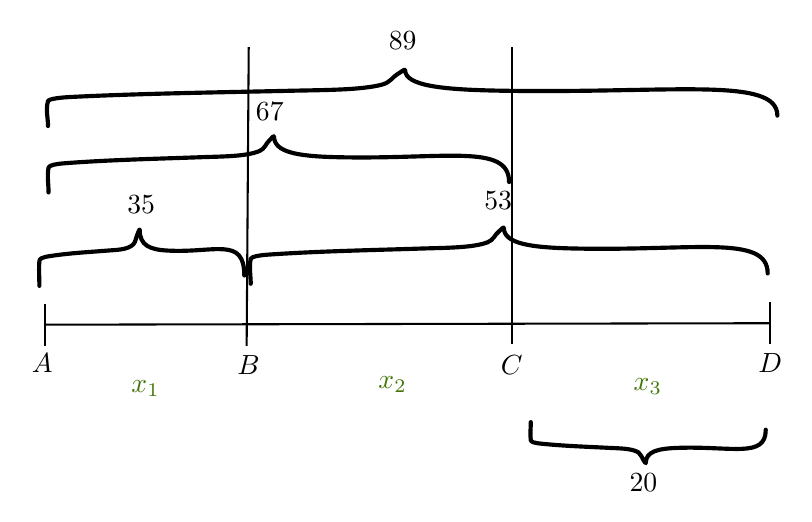
\begin{tikzpicture}[x=0.75pt,y=0.75pt,yscale=-1,xscale=1]
%uncomment if require: \path (0,300); %set diagram left start at 0, and has height of 300

%Straight Lines [id:da18809251009182648] 
\draw    (100,143) -- (449,142.29) ;
%Straight Lines [id:da4295294079118699] 
\draw    (100,132.85) -- (100,153.15) ;
%Straight Lines [id:da08559662247482214] 
\draw    (198,9.29) -- (197,153.15) ;
%Straight Lines [id:da8061715298122138] 
\draw    (325,9.29) -- (325,152.15) ;
%Straight Lines [id:da1891846903803609] 
\draw    (449,132.15) -- (449,152.44) ;
%Shape: Free Drawing [id:dp5156036617765727] 
\draw  [color={rgb, 255:red, 0; green, 0; blue, 0 }  ][line width=1.5] [line join = round][line cap = round] (101.3,47.29) .. controls (101.3,43.29) and (100.09,39.28) .. (101.3,35.29) .. controls (101.67,34.1) and (107.95,33.51) .. (112.28,33.29) .. controls (146.53,31.59) and (183.69,31.09) .. (218.43,30.29) .. controls (233.89,29.94) and (252.54,29.98) .. (262.36,27.29) .. controls (266.42,26.18) and (267.24,23.63) .. (269.68,22.29) .. controls (270.9,21.63) and (273.34,19.55) .. (273.34,20.29) .. controls (273.34,27.91) and (291.11,29.83) .. (320.92,30.29) .. controls (402.67,31.57) and (452.7,23.35) .. (452.7,42.29) ;
%Shape: Free Drawing [id:dp895862543035038] 
\draw  [color={rgb, 255:red, 0; green, 0; blue, 0 }  ][line width=1.5] [line join = round][line cap = round] (101.56,79.29) .. controls (101.56,75.29) and (100.79,71.28) .. (101.56,67.29) .. controls (101.79,66.1) and (105.76,65.51) .. (108.49,65.29) .. controls (130.11,63.59) and (153.58,63.09) .. (175.52,62.29) .. controls (185.28,61.94) and (197.06,61.98) .. (203.25,59.29) .. controls (205.82,58.18) and (206.34,55.63) .. (207.88,54.29) .. controls (208.65,53.63) and (210.19,51.55) .. (210.19,52.29) .. controls (210.19,59.91) and (221.41,61.83) .. (240.24,62.29) .. controls (291.85,63.57) and (323.44,55.35) .. (323.44,74.29) ;
%Shape: Free Drawing [id:dp019817472694717342] 
\draw  [color={rgb, 255:red, 0; green, 0; blue, 0 }  ][line width=1.5] [line join = round][line cap = round] (198.97,123.29) .. controls (198.97,119.29) and (198.11,115.28) .. (198.97,111.29) .. controls (199.23,110.1) and (203.69,109.51) .. (206.75,109.29) .. controls (231.03,107.59) and (257.37,107.09) .. (281.99,106.29) .. controls (292.94,105.94) and (306.17,105.98) .. (313.12,103.29) .. controls (316,102.18) and (316.58,99.63) .. (318.31,98.29) .. controls (319.18,97.63) and (320.91,95.55) .. (320.91,96.29) .. controls (320.91,103.91) and (333.5,105.83) .. (354.63,106.29) .. controls (412.57,107.57) and (448.03,99.35) .. (448.03,118.29) ;
%Shape: Free Drawing [id:dp36042969413065307] 
\draw  [color={rgb, 255:red, 0; green, 0; blue, 0 }  ][line width=1.5] [line join = round][line cap = round] (97.14,124.29) .. controls (97.14,120.29) and (96.8,116.28) .. (97.14,112.29) .. controls (97.24,111.1) and (99.01,110.51) .. (100.23,110.29) .. controls (109.85,108.59) and (120.29,108.09) .. (130.05,107.29) .. controls (134.39,106.94) and (139.63,106.98) .. (142.39,104.29) .. controls (143.53,103.18) and (143.76,100.63) .. (144.44,99.29) .. controls (144.79,98.63) and (145.47,96.55) .. (145.47,97.29) .. controls (145.47,104.91) and (150.46,106.83) .. (158.84,107.29) .. controls (181.8,108.57) and (195.86,100.35) .. (195.86,119.29) ;
%Shape: Free Drawing [id:dp5719345430074279] 
\draw  [color={rgb, 255:red, 0; green, 0; blue, 0 }  ][line width=1.5] [line join = round][line cap = round] (333.9,189.94) .. controls (333.9,192.86) and (333.5,195.79) .. (333.9,198.7) .. controls (334.01,199.57) and (336.04,200) .. (337.43,200.16) .. controls (348.47,201.4) and (360.44,201.77) .. (371.63,202.35) .. controls (376.61,202.6) and (382.62,202.58) .. (385.78,204.54) .. controls (387.09,205.35) and (387.35,207.21) .. (388.14,208.19) .. controls (388.53,208.67) and (389.32,210.19) .. (389.32,209.65) .. controls (389.32,204.09) and (395.05,202.69) .. (404.65,202.35) .. controls (430.99,201.42) and (447.1,207.42) .. (447.1,193.59) ;

% Text Node
\draw (92,155.4) node [anchor=north west][inner sep=0.75pt]    {$A$};
% Text Node
\draw (191,156.4) node [anchor=north west][inner sep=0.75pt]    {$B$};
% Text Node
\draw (318,156.4) node [anchor=north west][inner sep=0.75pt]    {$C$};
% Text Node
\draw (442,155.4) node [anchor=north west][inner sep=0.75pt]    {$D$};
% Text Node
\draw (140,168.4) node [anchor=north west][inner sep=0.75pt]  [color={rgb, 255:red, 65; green, 117; blue, 5 }  ,opacity=1 ]  {$x_{1}$};
% Text Node
\draw (259,166.4) node [anchor=north west][inner sep=0.75pt]  [color={rgb, 255:red, 65; green, 117; blue, 5 }  ,opacity=1 ]  {$x_{2}$};
% Text Node
\draw (382,167.4) node [anchor=north west][inner sep=0.75pt]  [color={rgb, 255:red, 65; green, 117; blue, 5 }  ,opacity=1 ]  {$x_{3}$};
% Text Node
\draw (264,0.4) node [anchor=north west][inner sep=0.75pt]    {$89$};
% Text Node
\draw (200,34.4) node [anchor=north west][inner sep=0.75pt]    {$67$};
% Text Node
\draw (310,77.4) node [anchor=north west][inner sep=0.75pt]    {$53$};
% Text Node
\draw (138,79.4) node [anchor=north west][inner sep=0.75pt]    {$35$};
% Text Node
\draw (380,213.4) node [anchor=north west][inner sep=0.75pt]    {$20$};


\end{tikzpicture}
\end{FigureCenter}

由 $ x_{1}, x_{2} $ 和 $ x_{3} $ 的关系可得方程组:
\begin{equation}
\left\{\begin{array}{r}
x_{1}+x_{2}+x_{3}=89 \\
x_{1}+x_{2}=67 \\
x_{2}+x_{3}=53 \\
x_{1}=35 \\
x_{3}=20
\end{array} \Leftrightarrow A x=b, A=\left[\begin{array}{lll}
1 & 1 & 1 \\
1 & 1 & 0 \\
0 & 1 & 1 \\
1 & 0 & 0 \\
0 & 0 & 1
\end{array}\right], b=\left[\begin{array}{l}
89 \\
67 \\
53 \\
35 \\
20
\end{array}\right]\right.
\end{equation}

取后三个式子求解方程组,回代前两个式子

\begin{equation}\displaystyle  \begin{array}{{>{\displaystyle}l}}
\left\{\begin{array}{ r }
x_{2} +x_{3} =53\\
x_{1} =35\\
x_{3} =20
\end{array} \Rightarrow x_{1} =35,x_{2} =33,x_{3} =20.\right. \\
\left\{\begin{array}{ r }
x_{1} +x_{2} +x_{3} =88\neq 89\\
x_{1} +x_{2} =68\neq 67
\end{array}\right. 
\end{array}\end{equation}
     

由于测量存在误差,方程组之间相互矛盾,该超定方程组无解。

\section{最小二乘问题}

\begin{problem}[最小二乘问题]
    寻找该方程组的近似解,并尽可能逼近方程组的目标$b$, 即残差向量 $ r=A x-b $ 某种度量下尽可能小

    \begin{equation} \min _{x}\|A x-b\|_{2}^{2}=\|r\|_{2}^{2} \quad (\ell_2范数度量残差) \end{equation}
\end{problem}


使用$\ell_1$、$\ell_\infty$等也可以度量误差,但是函数在零点处不光滑,不能求导。

\begin{problem}[求解最小二乘解]
    给定 $ {A} \in \mathfrak{R}^{m \times n}, {b} \in \mathfrak{R}^{m} $, 求解 $ x \in \mathfrak{R}^{n} $ 让目标函数最小

\begin{equation} \min _{x}\|A x-b\|_{2}^{2}=\min _{x} \sum_{i=1}^{m}\left(\sum_{j=1}^{n} A_{i j} x_{j}-b_{i}\right)^{2} \end{equation}
\end{problem}

\begin{notation}[最小二乘法的解]
    记最小二乘法的解为 $ \hat{x} $

    \begin{equation}
    \hat{x}=\arg \underset{x}{\min}\|A x-b\|_{2}^{2}=\arg \underset{x}{\min} \sum_{i=1}^{m}\left(\sum_{j=1}^{n} A_{i j} x_{j}-b_{i}\right)^{2}
    \end{equation}
\end{notation}

\begin{example}
    \begin{equation} f(x)=\|A x-b\|_{2}^{2}, {A}=\left[\begin{array}{cc}2 & 0 \\ -1 & 1 \\ 0 & 2\end{array}\right], b=\left[\begin{array}{c}1 \\ 0 \\ -1\end{array}\right] \end{equation}

    求解\begin{equation}\hat{x} = \arg \underset{x}{\min} \|A x-b\|_{2}^{2}\end{equation}

    解:
    \begin{equation} f(x)=\|A x-b\|_{2}^{2}=\left(2 x_{1}-1\right)^{2}+\left(-x_{1}+x_{2}\right)^{2}+\left(2 x_{2}+1\right)^{2} \end{equation}

    \begin{equation} \frac{\partial f}{\partial x_{1}}=10 x_{1}-2 x_{2}-4 , \frac{\partial f}{\partial x_{2}}=-2 x_{1}+10 x_{2}+4 \end{equation}

    \begin{equation} \nabla f(x)=\left[\begin{array}{l}\dfrac{\partial f}{\partial x_{1}} \\ \dfrac{\partial f}{\partial x_{2}}\end{array}\right]=0 \Rightarrow \hat{x}=\left(\frac{1}{3},-\frac{1}{3}\right)^{T} \end{equation}
\end{example}


\begin{theorem}
    设最小二乘法的解为 $ \hat{x} $ ,满足:
    \begin{equation}
    \|A \hat{x}-b\|_{2}^{2} \leq\|A x-b\|_{2}^{2}, \forall x \in \mathfrak{R}^{n}
    \end{equation}

    当残差 $ \hat{r}=A \hat{x}-b=0 $ 时,则 $ \hat{x} $ 是线性方程组 $ A x=b $ 的解; 否则其为误差最小平方和意义下方程组的近似解。
\end{theorem}



\section{求解最小二乘法}

给定 $ A \in \mathfrak{R}^{m \times n}, b \in \mathfrak{R}^{m}, x \in \mathfrak{R}^{n} $ 目标函数:
\begin{equation}
f(x)=\|A x-b\|_{2}^{2}=\sum_{i=1}^{m}\left(\sum_{j=1}^{n} A_{i j} x_{j}-b_{i}\right)^{2}
\end{equation}

为使目标函数最小,求最优解 $ \hat{x}:\hat{x}=\arg \underset{x}{\min} f(x) $

\begin{theorem}
    可微函数 $ f(x) $ 的最优解 $ \hat{x} $ 满足条件:梯度 $ \nabla f(\hat{x})=\mathbf{0} $ , 即:
\begin{equation}
\nabla f(\hat{x})=\left[\begin{array}{c}
\dfrac{\partial f}{\partial x_{1}}(\hat{x}) \\
\vdots \\
\dfrac{\partial f}{\partial x_{n}}(\hat{x})
\end{array}\right]=2 A^{T}(A \hat{x}-b)=0
\end{equation}
\end{theorem}

利用上面这个定理,可以推导出正规方程和最小二乘解。

\begin{theorem}[正规方程与最小二乘解]
    \begin{equation} A^{T} A x=A^{T} b \end{equation}

    $A$的列向量\textbf{线性无关}时,则 $ \hat{x}=\left(A^{T} A\right)^{-1} A^{T} b $. 
\end{theorem}

\begin{proof}
    设函数 $ g_{i}(x)=\sum_{j=1}^{n} A_{i j} x_{j}-b_{i} $ ,则有

    
        \begin{equation}g_{i}( x) =\sum\limits _{j=1}^{n} A_{ij} x_{j} -b_{i} \Rightarrow \left(\begin{array}{ c c c c c }
        A_{1,1} & \cdots  & A_{1,k} & \cdots  & A_{1,n}\\
        \vdots  &  & \vdots  &  & \vdots \\
        \boldsymbol{\textcolor[rgb]{0.72,0.33,0.31}{A}\textcolor[rgb]{0.72,0.33,0.31}{_{j,1}}} & \boldsymbol{\textcolor[rgb]{0.72,0.33,0.31}{\cdots }} & \boldsymbol{\textcolor[rgb]{0.72,0.33,0.31}{A}\textcolor[rgb]{0.72,0.33,0.31}{_{j,k}}} & \boldsymbol{\textcolor[rgb]{0.72,0.33,0.31}{\cdots }} & \boldsymbol{\textcolor[rgb]{0.72,0.33,0.31}{A}\textcolor[rgb]{0.72,0.33,0.31}{_{j,n}}}\\
        \vdots  &  & \vdots  &  & \vdots \\
        A_{m,1} & \cdots  & A_{m,k} & \cdots  & A_{m,n}
        \end{array}\right)\left(\begin{array}{ c }
        \boldsymbol{\textcolor[rgb]{0.72,0.33,0.31}{x}\textcolor[rgb]{0.72,0.33,0.31}{_{1}}}\\
        \boldsymbol{\textcolor[rgb]{0.72,0.33,0.31}{\vdots }}\\
        \boldsymbol{\textcolor[rgb]{0.72,0.33,0.31}{x}\textcolor[rgb]{0.72,0.33,0.31}{_{j}}}\\
        \boldsymbol{\textcolor[rgb]{0.72,0.33,0.31}{\vdots }}\\
        \boldsymbol{\textcolor[rgb]{0.72,0.33,0.31}{x}\textcolor[rgb]{0.72,0.33,0.31}{_{n}}}
        \end{array}\right) -\left(\begin{array}{ c }
        \textcolor[rgb]{0,0,0}{b_{1}}\\
        \textcolor[rgb]{0,0,0}{\vdots }\\
        \textcolor[rgb]{0.72,0.33,0.31}{b\boldsymbol{_{j}}}\\
        \textcolor[rgb]{0,0,0}{\vdots }\\
        \textcolor[rgb]{0,0,0}{b_{n}}
        \end{array}\right)\end{equation}
    
    所以
    \begin{equation}\begin{aligned} 
        f(x)&=\|A x-b\|_{2}^{2}
        &=\sum_{i=1}^{m}\left(\sum_{j=1}^{n} A_{i j} x_{j}-b_{i}\right)^{2}
        &=\sum_{i=1}^{m}\left(g_{i}(x)\right)^{2} 
    \end{aligned}\end{equation}

    函数 $ f(x) $ 对变量 $ x_{k} $ 偏导为
    
    \begin{equation} \frac{\partial f(x)}{\partial x_{k}}=\sum_{i=1}^{m}\left(\left(2 g_{i}(x)\right)\left(\frac{\partial g_{i}(x)}{\partial x_{k}}\right)\right) \end{equation}


    又因为
    \begin{equation} \frac{\partial g_{i}(x)}{\partial x_{k}}=A_{i k} \end{equation}


    所以
    \begin{equation} \begin{aligned} 
        \frac{\partial f}{\partial x_{k}}(x) 
        &=\sum_{i=1}^{m} 2\left(g_{i}(x)\right)\left(A_{i k}\right) \\
        &=2 \sum_{i=1}^{m}\left(\left(\sum_{j=1}^{n} A_{i j} x_{j}-b_{i}\right)\left(A_{i k}\right)\right) 
        \\ &=2 \sum_{i=1}^{m}\left(\left(\sum_{j=1}^{n} A_{i j} x_{j}\right)\left(A_{i k}\right)\right)-2 \sum_{i=1}^{m}\left(\left(b_{i}\right)\left(A_{i k}\right)\right) \end{aligned} \end{equation}

    注意有
        

    \begin{equation}\sum\limits _{j=1}^{n} A_{ij} x_{j} \Rightarrow 
    \left(\begin{array}{ c c c c c }
    A_{1,1} & \cdots  & A_{1,k} & \cdots  & A_{1,n}\\
    \vdots  &  & \vdots  &  & \vdots \\
    \boldsymbol{\textcolor[rgb]{0.72,0.33,0.31}{A}\textcolor[rgb]{0.72,0.33,0.31}{_{i,1}}} & \boldsymbol{\textcolor[rgb]{0.72,0.33,0.31}{\cdots }} & \boldsymbol{\textcolor[rgb]{0.72,0.33,0.31}{A}\textcolor[rgb]{0.72,0.33,0.31}{_{i,k}}} & \boldsymbol{\textcolor[rgb]{0.72,0.33,0.31}{\cdots }} & \boldsymbol{\textcolor[rgb]{0.72,0.33,0.31}{A}\textcolor[rgb]{0.72,0.33,0.31}{_{i,n}}}\\
    \vdots  &  & \vdots  &  & \vdots \\
    A_{m,1} & \cdots  & A_{m,k} & \cdots  & A_{m,n}
    \end{array}\right)\left(\begin{array}{ c }
    \boldsymbol{\textcolor[rgb]{0.72,0.33,0.31}{x}\textcolor[rgb]{0.72,0.33,0.31}{_{1}}}\\
    \boldsymbol{\textcolor[rgb]{0.72,0.33,0.31}{\vdots }}\\
    \boldsymbol{\textcolor[rgb]{0.72,0.33,0.31}{x}\textcolor[rgb]{0.72,0.33,0.31}{_{i}}}\\
    \boldsymbol{\textcolor[rgb]{0.72,0.33,0.31}{\vdots }}\\
    \boldsymbol{\textcolor[rgb]{0.72,0.33,0.31}{x}\textcolor[rgb]{0.72,0.33,0.31}{_{n}}}
    \end{array}\right) =\left(\begin{array}{ c }
    Result_{1}\\
    \vdots \\
    \boldsymbol{\textcolor[rgb]{0.72,0.33,0.31}{Result}\textcolor[rgb]{0.72,0.33,0.31}{_{i}}}\\
    \vdots \\
    Result_{m}
    \end{array}\right) =Ax\end{equation}

    \begin{remark}
        在此处$i$是自由变量。
    \end{remark}

    \begin{equation}\displaystyle \sum _{i=1}^{m}\left(\underbrace{\left(\sum _{j=1}^{n} A_{ij} x_{j}\right)}_{Result}( A_{ik})\right) =\begin{array}{ c }
    A_{1,\textcolor[rgb]{0.29,0.56,0.89}{\boldsymbol{k}}} \times Result_{1}\\
    +\\
    \vdots \\
    +\\
    \boldsymbol{\textcolor[rgb]{0.72,0.33,0.31}{A_{i,\textcolor[rgb]{0.29,0.56,0.89}{\boldsymbol{k}}} \times Result}\textcolor[rgb]{0.72,0.33,0.31}{_{i}}}\\
    +\\
    \vdots \\
    +\\
    A\textcolor[rgb]{0.29,0.56,0.89}{\boldsymbol{_{\textcolor[rgb]{0,0,0}{m,} k}}} \times Result_{m}
    \end{array} =\left(\begin{array}{ c }
    A_{1,\textcolor[rgb]{0.29,0.56,0.89}{\boldsymbol{k}}}\\
    \vdots \\
    A_{i,\textcolor[rgb]{0.29,0.56,0.89}{\boldsymbol{k}}}\\
    \vdots \\
    A_{m,\textcolor[rgb]{0.29,0.56,0.89}{\boldsymbol{k}}}
    \end{array}\right)^{T} Ax=a_{\textcolor[rgb]{0.29,0.56,0.89}{\boldsymbol{k}}}^{T} Ax\end{equation}
        
    类似地,有 
    
    \begin{equation}\displaystyle \sum _{i=1}^{m}(( b_{i})( A_{ik})) =\begin{array}{ c }
    A_{1,\textcolor[rgb]{0.29,0.56,0.89}{\boldsymbol{k}}} \times b_{1}\\
    +\\
    \vdots \\
    +\\
    \boldsymbol{\textcolor[rgb]{0.72,0.33,0.31}{A}\textcolor[rgb]{0.72,0.33,0.31}{_{i,\textcolor[rgb]{0.29,0.56,0.89}{\boldsymbol{k}}}}\textcolor[rgb]{0.72,0.33,0.31}{\times b}\textcolor[rgb]{0.72,0.33,0.31}{_{i}}}\\
    +\\
    \vdots \\
    +\\
    A\textcolor[rgb]{0.29,0.56,0.89}{\boldsymbol{_{\textcolor[rgb]{0,0,0}{m,} k}}} \times b_{m}
    \end{array} =a_{\textcolor[rgb]{0.29,0.56,0.89}{\boldsymbol{k}}}^{T} b\end{equation}
        
    所以
    \begin{equation}
    \begin{aligned}
        \frac{\partial f}{\partial x_{k}}(x)
        &=2 a_{k}^{T} A x-2 a_{k}^{T} b\\
        &=2 a_{k}^{T}(A x-b)
    \end{aligned}
    \end{equation}

    所以函数 $ f(x) $ 的梯度
\begin{equation}
\begin{aligned}
    \nabla f(x)&=\left[\begin{array}{c}
    \dfrac{\partial f}{\partial x_{1}}(x) \\
    \vdots \\
    \dfrac{\partial f}{\partial x_{n}}(x)
    \end{array}\right]\\
    &=2\left[\begin{array}{c}
    a_{1}^{T}(A x-b) \\
    a_{2}^{T}(A x-b) \\
    \vdots \\
    a_{n}^{T}(A x-b)
    \end{array}\right] \\
    &= 2\left[a_{1}, a_{2}, \cdots, a_{n}\right]^{T}(A x-b) \\
    &=2 A^{T}(A x-b) 
\end{aligned}
\end{equation}

令梯度等于0
\begin{equation}\nabla f(x)=2\left(A^{T} A x-A^{T} b\right)=0 \Rightarrow A^{T} A x=A^{T} b\end{equation}

$A$的列向量无关时,则 $ \hat{x}=\left(A^{T} A\right)^{-1} A^{T} b $.

\end{proof}

\section{The Geometry of Least Squares: 投影与$A$列空间的关系}

\begin{FigureCenter}{Projection of $\boldsymbol{b}$ into the column space of ${A}$, $A$ is any matrice. Sourced from \cite{Strang1993IntroductionTL}}
    \tikzset{every picture/.style={line width=0.75pt}} %set default line width to 0.75pt        

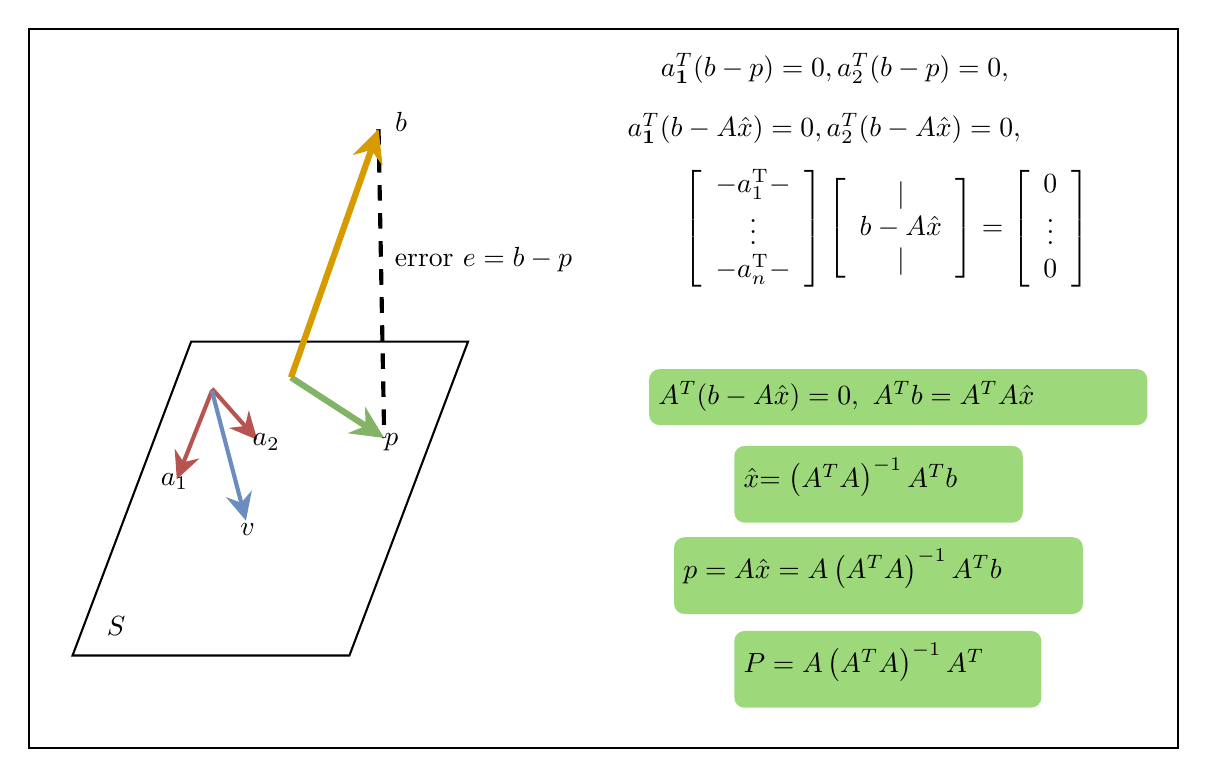
\begin{tikzpicture}[x=0.75pt,y=0.75pt,yscale=-1,xscale=1]
%uncomment if require: \path (0,350); %set diagram left start at 0, and has height of 350

%Straight Lines [id:da0833896477217686] 
\draw [color={rgb, 255:red, 130; green, 179; blue, 102 }  ,draw opacity=1 ][line width=2.25]    (127.38,169.03) -- (168.08,195.47) ;
\draw [shift={(172.28,198.19)}, rotate = 213] [fill={rgb, 255:red, 130; green, 179; blue, 102 }  ,fill opacity=1 ][line width=0.08]  [draw opacity=0] (16.07,-7.72) -- (0,0) -- (16.07,7.72) -- (10.67,0) -- cycle    ;
%Straight Lines [id:da7639150841734914] 
\draw [color={rgb, 255:red, 184; green, 84; blue, 80 }  ,draw opacity=1 ][line width=1.5]    (89.28,175.43) -- (73.82,214.38) ;
\draw [shift={(72.35,218.1)}, rotate = 291.64] [fill={rgb, 255:red, 184; green, 84; blue, 80 }  ,fill opacity=1 ][line width=0.08]  [draw opacity=0] (13.4,-6.43) -- (0,0) -- (13.4,6.44) -- (8.9,0) -- cycle    ;
%Straight Lines [id:da3617082286190523] 
\draw [line width=1.5]  [dash pattern={on 5.63pt off 4.5pt}]  (169.55,49.34) -- (172.28,198.19) ;
%Shape: Parallelogram [id:dp7592583426452624] 
\draw   (79.28,151.73) -- (212.68,151.73) -- (155.51,303) -- (22.11,303) -- cycle ;
%Straight Lines [id:da8449665178781662] 
\draw [color={rgb, 255:red, 184; green, 84; blue, 80 }  ,draw opacity=1 ][line width=1.5]    (89.28,174.43) -- (108.47,196.09) ;
\draw [shift={(111.12,199.08)}, rotate = 228.46] [fill={rgb, 255:red, 184; green, 84; blue, 80 }  ,fill opacity=1 ][line width=0.08]  [draw opacity=0] (13.4,-6.43) -- (0,0) -- (13.4,6.44) -- (8.9,0) -- cycle    ;
%Straight Lines [id:da21760172692551993] 
\draw [color={rgb, 255:red, 106; green, 140; blue, 190 }  ,draw opacity=1 ][line width=1.5]    (89.28,175.43) -- (104.64,234.14) ;
\draw [shift={(105.66,238.01)}, rotate = 255.32999999999998] [fill={rgb, 255:red, 106; green, 140; blue, 190 }  ,fill opacity=1 ][line width=0.08]  [draw opacity=0] (13.4,-6.43) -- (0,0) -- (13.4,6.44) -- (8.9,0) -- cycle    ;
%Straight Lines [id:da9743594112783229] 
\draw [color={rgb, 255:red, 215; green, 155; blue, 0 }  ,draw opacity=1 ][line width=2.25]    (127.38,169.03) -- (167.89,54.06) ;
\draw [shift={(169.55,49.34)}, rotate = 469.41] [fill={rgb, 255:red, 215; green, 155; blue, 0 }  ,fill opacity=1 ][line width=0.08]  [draw opacity=0] (16.07,-7.72) -- (0,0) -- (16.07,7.72) -- (10.67,0) -- cycle    ;
%Shape: Rectangle [id:dp3830905409317218] 
\draw   (1,1) -- (554.64,1) -- (554.64,347.62) -- (1,347.62) -- cycle ;

% Text Node
\draw (175.98,39.87) node [anchor=north west][inner sep=0.75pt]    {$\boldsymbol{b}$};
% Text Node
\draw (170.85,194.49) node [anchor=north west][inner sep=0.75pt]    {$\boldsymbol{p}$};
% Text Node
\draw (107.38,194.77) node [anchor=north west][inner sep=0.75pt]    {$\boldsymbol{a}_{2}$};
% Text Node
\draw (175.92,104.86) node [anchor=north west][inner sep=0.75pt]   [align=left] {error $\displaystyle \boldsymbol{e} =\boldsymbol{b-p}$};
% Text Node
\draw (63.21,213.92) node [anchor=north west][inner sep=0.75pt]    {$\boldsymbol{a}_{1}$};
% Text Node
\draw (101.48,237.88) node [anchor=north west][inner sep=0.75pt]    {$\boldsymbol{v}$};
% Text Node
\draw (37.18,282.9) node [anchor=north west][inner sep=0.75pt]    {$\boldsymbol{S}$};
% Text Node
\draw (288.11,40.4) node [anchor=north west][inner sep=0.75pt]    {$\boldsymbol{a}_{\mathbf{1}}^{T} (\boldsymbol{b} -\boldsymbol{A}\hat{\boldsymbol{x}} )=0,\boldsymbol{a}_{2}^{T} (\boldsymbol{b} -\boldsymbol{A}\hat{\boldsymbol{x}} )=0,\dotsc $};
% Text Node
\draw (304.11,11.4) node [anchor=north west][inner sep=0.75pt]    {$\boldsymbol{a}_{\mathbf{1}}^{T} (\boldsymbol{b} -\boldsymbol{p} )=0,\boldsymbol{a}_{2}^{T} (\boldsymbol{b} -\boldsymbol{p} )=0,\dotsc $};
% Text Node
\draw (314.93,67.4) node [anchor=north west][inner sep=0.75pt]    {$\left[\begin{array}{ c }
-\boldsymbol{a}_{1}^{\mathrm{T}} -\\
\vdots \\
-\boldsymbol{a}_{n}^{\mathrm{T}} -
\end{array}\right]\left[\begin{array}{ c }
\mid \\
\boldsymbol{b} -\boldsymbol{A\hat{\boldsymbol{x}}}\\
\mid 
\end{array}\right] =\left[\begin{array}{ c }
0\\
\vdots \\
0
\end{array}\right]$};
% Text Node
\draw  [color={rgb, 255:red, 0; green, 0; blue, 0 }  ,draw opacity=0 ][fill={rgb, 255:red, 157; green, 217; blue, 123 }  ,fill opacity=1 ]  (299.93,170) .. controls (299.93,167.24) and (302.17,165) .. (304.93,165) -- (534.93,165) .. controls (537.7,165) and (539.93,167.24) .. (539.93,170) -- (539.93,187) .. controls (539.93,189.76) and (537.7,192) .. (534.93,192) -- (304.93,192) .. controls (302.17,192) and (299.93,189.76) .. (299.93,187) -- cycle  ;
\draw (302.93,169.4) node [anchor=north west][inner sep=0.75pt]    {$\boldsymbol{A^{T} (b-A\hat{x} )} =0,\ \boldsymbol{A^{T} b=A^{T} A\hat{x}}$};
% Text Node
\draw  [color={rgb, 255:red, 0; green, 0; blue, 0 }  ,draw opacity=0 ][fill={rgb, 255:red, 157; green, 217; blue, 123 }  ,fill opacity=1 ]  (340.93,207) .. controls (340.93,204.24) and (343.17,202) .. (345.93,202) -- (474.93,202) .. controls (477.7,202) and (479.93,204.24) .. (479.93,207) -- (479.93,234) .. controls (479.93,236.76) and (477.7,239) .. (474.93,239) -- (345.93,239) .. controls (343.17,239) and (340.93,236.76) .. (340.93,234) -- cycle  ;
\draw (343.93,206.4) node [anchor=north west][inner sep=0.75pt]    {$\hat{\boldsymbol{x}}\boldsymbol{=\left( A^{T} A\right)^{-1} A^{T} b}$};
% Text Node
\draw  [color={rgb, 255:red, 157; green, 217; blue, 123 }  ,draw opacity=0 ][fill={rgb, 255:red, 157; green, 217; blue, 123 }  ,fill opacity=1 ]  (311.93,251) .. controls (311.93,248.24) and (314.17,246) .. (316.93,246) -- (503.93,246) .. controls (506.7,246) and (508.93,248.24) .. (508.93,251) -- (508.93,278) .. controls (508.93,280.76) and (506.7,283) .. (503.93,283) -- (316.93,283) .. controls (314.17,283) and (311.93,280.76) .. (311.93,278) -- cycle  ;
\draw (314.93,250.4) node [anchor=north west][inner sep=0.75pt]    {$\boldsymbol{p=A\hat{x} =A\left( A^{T} A\right)^{-1} A^{T} b}$};
% Text Node
\draw  [color={rgb, 255:red, 0; green, 0; blue, 0 }  ,draw opacity=0 ][fill={rgb, 255:red, 157; green, 217; blue, 123 }  ,fill opacity=1 ]  (340.93,296.15) .. controls (340.93,293.38) and (343.17,291.15) .. (345.93,291.15) -- (483.93,291.15) .. controls (486.7,291.15) and (488.93,293.38) .. (488.93,296.15) -- (488.93,323.15) .. controls (488.93,325.91) and (486.7,328.15) .. (483.93,328.15) -- (345.93,328.15) .. controls (343.17,328.15) and (340.93,325.91) .. (340.93,323.15) -- cycle  ;
\draw (343.93,295.55) node [anchor=north west][inner sep=0.75pt]    {$\boldsymbol{P=A\left( A^{T} A\right)^{-1} A^{T}}$};


\end{tikzpicture}

\end{FigureCenter}

\begin{FigureCenter}{Projecting onto the column space of $A$ is also projecting onto the column space of $Q$}
    \tikzset{every picture/.style={line width=0.75pt}} %set default line width to 0.75pt

\begin{tikzpicture}[x=0.75pt,y=0.75pt,yscale=-1,xscale=1]
%uncomment if require: \path (0,300); %set diagram left start at 0, and has height of 300

%Shape: Parallelogram [id:dp16734778977883136] 
\draw  [color={rgb, 255:red, 255; green, 255; blue, 255 }  ,draw opacity=1 ][fill={rgb, 255:red, 179; green, 179; blue, 179 }  ,fill opacity=1 ] (224.15,98.88) -- (563.14,98.88) -- (417.85,242.95) -- (78.86,242.95) -- cycle ;
%Straight Lines [id:da3519715103345966] 
\draw [color={rgb, 255:red, 0; green, 0; blue, 0 }  ,draw opacity=1 ][line width=1.5]  [dash pattern={on 1.69pt off 2.76pt}]  (399.96,59.43) -- (399.07,151.88) ;
%Straight Lines [id:da7143500773565701] 
\draw [color={rgb, 255:red, 74; green, 144; blue, 226 }  ,draw opacity=1 ][line width=2.25]    (252.07,166.88) -- (395.92,62.37) ;
\draw [shift={(399.96,59.43)}, rotate = 504] [fill={rgb, 255:red, 74; green, 144; blue, 226 }  ,fill opacity=1 ][line width=0.08]  [draw opacity=0] (14.29,-6.86) -- (0,0) -- (14.29,6.86) -- cycle    ;
%Straight Lines [id:da29623635442698415] 
\draw [color={rgb, 255:red, 234; green, 81; blue, 100 }  ,draw opacity=1 ][line width=2.25]    (252.07,166.88) -- (394.09,152.39) ;
\draw [shift={(399.07,151.88)}, rotate = 534.1700000000001] [fill={rgb, 255:red, 234; green, 81; blue, 100 }  ,fill opacity=1 ][line width=0.08]  [draw opacity=0] (14.29,-6.86) -- (0,0) -- (14.29,6.86) -- cycle    ;

% Text Node
\draw (114.72,185.99) node [anchor=north west][inner sep=0.75pt]    {$\begin{aligned}
C( A) & =C( Q)\\
\operatorname{range}( A) & =\operatorname{range}( Q)
\end{aligned}$};
% Text Node
\draw (376.21,43.4) node [anchor=north west][inner sep=0.75pt]    {$x$};
% Text Node
\draw  [color={rgb, 255:red, 0; green, 0; blue, 0 }  ,draw opacity=0 ][fill={rgb, 255:red, 234; green, 81; blue, 100 }  ,fill opacity=1 ]  (347.57,167.38) .. controls (347.57,164.62) and (349.8,162.38) .. (352.57,162.38) -- (463.57,162.38) .. controls (466.33,162.38) and (468.57,164.62) .. (468.57,167.38) -- (468.57,182.38) .. controls (468.57,185.14) and (466.33,187.38) .. (463.57,187.38) -- (352.57,187.38) .. controls (349.8,187.38) and (347.57,185.14) .. (347.57,182.38) -- cycle  ;
\draw (350.57,166.78) node [anchor=north west][inner sep=0.75pt]    {$AA^{\dagger } x=QQ^{T} x$};


\end{tikzpicture}
\end{FigureCenter}

矩阵 $ {A} \in \mathfrak{R}^{m \times n} $ 的列 $ a_{1}, a_{2}, \ldots, a_{n} \in \mathfrak{R}^{m} $ 的最小二乘法问题
\begin{equation}
\hat{x}=\arg \underset{x}{\min}\|A x-b\|_{2}^{2} ,\|A x-b\|_{2}^{2}=\left\|\sum_{j=1}^{n} a_{j} x_{j}-b\right\|_{2}^{2}
\end{equation}

向量 $ b $ 在 $ \operatorname{range}(A) $ 上的投影是 $ A\left(A^{T} A\right)^{-1} A^{T} b $.

残差向量 $ \hat{r}=A \hat{x}-b $ 满足 $ A^{T} \hat{r}=A^{T}(A \hat{x}-b)=0 $.残差向量 $ \hat{r} $ 正交于 $ A $ 的每一列,因此正交于$ \operatorname{range}(A) $.




\begin{theorem}[投影与$A$列空间的关系]
    $ A \hat{x} \in \operatorname{range}(A) $是$A$的列空间中最接近$b$的向量。 
    
    $ \hat{r}=A \hat{x} -b$正交于$A$的列空间(值域空间) $ \operatorname{range}(A) $.
\end{theorem}

\section{正规方程}

\begin{theorem}[最小二乘法问题的正规方程]

    \begin{equation} \nabla f(x)=0, f(x)=\|A x-b\|_{2}^{2} \end{equation}
等价于
\begin{equation}
A^{T} A x=A^{T} b
\end{equation}
\end{theorem}

系数矩阵 $ A^{T} A $ 是 $ A $ 的Gram矩阵,最小二乘法问题所有的解都满足正规方程。

\begin{theorem}
    如果$A$的列线性无关,则

    $ A^{T} A $ 为非奇异矩阵,正规方程此时有唯一解。
\end{theorem}


\section{QR分解求解最小二乘法}

\begin{theorem}[QR分解求解最小二乘法]
    若 $ {A} \in \mathfrak{R}^{m \times n} $ 的列向量线性无关,则存在 $ {A}={QR} $ 分解, $ Q \in \mathfrak{R}^{m \times n} $ , $ R \in \mathfrak{R}^{{n} \times n} $ 
    
    最小二乘法问题的解
\begin{equation}
\begin{aligned}
\hat{x}&=\left(A^{T} A\right)^{-1} A^{T} b \\
&=\left((Q R)^{T}(Q R)\right)^{-1}(Q R)^{T} b \\
&=\left(R^{T} Q^{T} Q R\right)^{-1} R^{T} Q^{T} b \\
&=\left(R^{T} R\right)^{-1} R^{T} Q^{T} b \\
&=R^{-1} Q^{T} b
\end{aligned}
\end{equation}
\end{theorem}


\begin{example}
    \begin{equation}
A=\left[\begin{array}{cc}
3 & -6 \\
4 & -8 \\
0 & 1
\end{array}\right], \quad b=\left[\begin{array}{c}
-1 \\
7 \\
0
\end{array}\right]
\end{equation}
首先对$A$进行QR分解
\begin{equation}
Q=\left[\begin{array}{cc}
3 / 5 & 0 \\
4 / 5 & 0 \\
0 & 1
\end{array}\right], \quad R=\left[\begin{array}{cc}
5 & -10 \\
0 & 1
\end{array}\right]
\end{equation}

计算 $ d=Q^{T} b=(5,2) $

求解 $ R x=d $
\begin{equation}
\left[\begin{array}{cc}
5 & -10 \\
0 & 1
\end{array}\right]\left[\begin{array}{l}
x_{1} \\
x_{2}
\end{array}\right]=\left[\begin{array}{l}
5 \\
2
\end{array}\right]
\end{equation}

解得 $ x_{1}=5, x_{2}=2 $

\end{example}


\subsection{The Complexity of Solving Least Square Problem via QR Decomposition}
\label{complexity:least-square-using-qr}

算法复杂度:

\begin{itemize}
    \item 首先对$A$进行QR分解 $ A=Q R\left(2 m n^{2}\right. $ flops $ ) $
    \item 计算矩阵向量乘积 $ d=Q^{T} b(2 {mn} $ flops $ ) $
    \item 通过回代求解 $ R x=d\left(n^{2}\right. $ flops $ ) $
    \item 复杂度: $ 2 m n^{2} $ flops
\end{itemize}



\section{求解正规方程可能带来的严重误差}

直接求解正规方程组求解:
\begin{equation}
A^{T} A x=A^{T} b
\end{equation}

可能会造成严重的舍入误差。

\begin{example}
    一个列向量“几乎”线性相关的矩阵
\begin{equation}
A=\left[\begin{array}{cc}
1 & -1 \\
0 & 10^{-5} \\
0 & 0
\end{array}\right],  b=\left[\begin{array}{c}
0 \\
10^{-5} \\
1
\end{array}\right]
\end{equation}

将中间结果四舍五入到小数点后8位。

方法 1 :通过Gram矩阵求解
\begin{equation}
A^{T} A=\left[\begin{array}{cc}
1 & -1 \\
-1 & 1+10^{-10}
\end{array}\right] \approx\left[\begin{array}{cc}
1 & -1 \\
-1 & 1
\end{array}\right], A^{T} b=\left[\begin{array}{c}
0 \\
10^{-10}
\end{array}\right] \Rightarrow x=\left[\begin{array}{c}
10^{-10} \\
10^{-10}
\end{array}\right]
\end{equation}
经过四舍五入之后,Gram矩阵为奇异矩阵。


方法 2 : 通过对 $A$进行QR分解
\begin{equation}
Q=\left[\begin{array}{ll}
1 & 0 \\
0 & 1 \\
0 & 0
\end{array}\right],  R=\left[\begin{array}{cc}
1 & -1 \\
0 & 10^{-5}
\end{array}\right]
\end{equation}

\begin{equation}\begin{aligned}
    &\hat{x}=\left(A^{T} A\right)^{-1} A^{T} b=R^{-1} Q^{T} b \\
    \Rightarrow& R x=Q^{T} b\\
    \Rightarrow& \left[\begin{array}{cc}1 & -1 \\ 0 & 10^{-5}\end{array}\right]\left[\begin{array}{l}x_{1} \\ x_{2}\end{array}\right]=\left[\begin{array}{l}0 \\ 10^{-5}\end{array}\right] \\
    \Rightarrow& x=\left[\begin{array}{l}1 \\ 1\end{array}\right]
\end{aligned}\end{equation}

\end{example}

方法2 比方法1更稳定,因为它避免构造Gram矩阵。



\section{梯度下降法}

给定 $ A \in \mathfrak{R}^{m \times n}, {b} \in \mathfrak{R}^{m}, x \in \mathfrak{R}^{n} $ 目标函数:
\begin{equation}
f(x)=\|A x-b\|_{2}^{2}=\sum_{i=1}^{m}\left(\sum_{j=1}^{n} A_{i j} x_{j}-b_{i}\right)^{2}
\end{equation}
为使目标函数最小, 可求最优解 $ \hat{x}: \quad \hat{x}=\arg \underset{x}{ \min } f(x) $.

\begin{problem}
    $ A \in \mathfrak{R}^{{m} \times n} $ 列向量线性相关或$n$非常大,$
    A^{T} A \in \mathfrak{R}^{n \times n}$不可逆,无法直接代入求得最小二乘解。
\end{problem}

通过迭代求解目标的最优解过程: \begin{equation} x^{(1)}, x^{(2)}, \cdots, x^{(k)} \rightarrow \hat{x} \end{equation} 

设 $ x^{(k)} $ 是第$k$步迭代,期望更新 $ x^{(k+1)} $ ,满足 $ f\left(x^{(k+1)}\right)<f\left(x^{(k)}\right) $.

设函数 $ f(x) $ 可微,根据泰勒公式,在 $ x^{(k)} $ 的一阶公式为
\begin{equation}
f\left(x^{(k+1)}\right)=f\left(x^{(k)}\right)+\left\langle\nabla f\left(x^{(k)}\right), x^{(k+1)}-x^{(k)}\right\rangle+o\left(\left\|x^{(k+1)}-x^{(k)}\right\|\right)
\end{equation}

如果 $ \left\|x^{(k+1)}-x^{(k)}\right\|_{2} $ 足够小, 则有
\begin{equation}
f\left(x^{(k+1)}\right)-f\left(x^{(k)}\right) \approx\left\langle\nabla f\left(x^{(k)}\right), x^{(k+1)}-x^{(k)}\right\rangle
\end{equation}

\begin{corollary}
    根据Cauchy-Schwarz不等式 \ref{thm:cauchy-schwartz=inequality}

    $ \left|\left\langle\nabla f\left(x^{(k)}\right), x^{(k+1)}-x^{(k)}\right\rangle\right| \leq\left\|\nabla f\left(x^{(k)}\right)\right\|_{2}\left\|x^{(k+1)}-x^{(k)}\right\|_{2} $

    所以有
    \begin{equation}
\left\langle\nabla f\left(x^{(k)}\right), x^{(k+1)}-x^{(k)}\right\rangle \geq -\left\|\nabla f\left(x^{(k)}\right)\right\|_{2}\left\|x^{(k+1)}-x^{(k)}\right\|_{2}
\end{equation}

当 $ x^{(k+1)}-x^{(k)}=-\alpha_{k} \nabla f\left(x^{(k)}\right), \alpha_{k}>0 $ 时,等式成立。

由于$-\left\|\nabla f\left(x^{(k)}\right)\right\|_{2}\left\|x^{(k+1)}-x^{(k)}\right\|_{2}$是非负的,此时$f\left(x^{(k+1)}\right)-f\left(x^{(k)}\right) \le 0$.
\end{corollary}

迭代公式为 

\begin{equation}  x^{(k+1)}=x^{(k)}-\alpha_{k} \nabla f\left(x^{(k)}\right) , f\left(x^{(k+1)}\right)<f\left(x^{(k)}\right) \end{equation}


\begin{definition}[梯度下降法求解最小二乘法]
    \begin{equation}
\min _{x \in \mathfrak{R}^{n}} \frac{1}{2}\|A x-b\|_{2}^{2}, \quad A \in \mathfrak{R}^{m \times n}, b \in \mathfrak{R}^{m}
\end{equation}

令 \begin{equation} f(x)=\frac{1}{2}\|A x-b\|_{2}^{2} \end{equation}

则 $ f $ 为凸函数, 并有 $ \nabla f(x)=A^{T}(A x-b) $.

则 $ A^{T} A \in \mathfrak{R}^{n \times n} $ .如果列向量\textbf{线性相关}会导致其\textbf{不可逆}或$n$非常大。可以通过梯度下降法迭代

\begin{equation}  x^{(k+1)}=x^{(k)}-\alpha_{k} \nabla f\left(x^{(k)}\right) , f\left(x^{(k+1)}\right)<f\left(x^{(k)}\right) \end{equation}

求解

\begin{equation} x^{(k+1)}=x^{(k)}-\alpha^{(k)} A^{T}\left(A x^{(k)}-b\right) \end{equation}
\end{definition}


\begin{algorithm}[htbp]
    \caption{梯度下降法}
    初始化 $ x^{(0)} $, $k=0$\;
    \While(){Not Convergent}{
        $p^{(k)}=A^{T}\left(A x^{(k)}-b\right)$\;
        $x^{(k+1)}=x^{(k)}-\alpha^{(k)} p^{(k)}$\;
        $k \leftarrow k + 1$
    }
\end{algorithm}

\section{估计学习率(步长)$\alpha$}

\begin{problem}
    \begin{equation}
    \min _{x \in \mathfrak{R}^{n}} \frac{1}{2}\|A x-b\|_{2}^{2}, \quad A \in \mathfrak{R}^{m \times n}, b \in \mathfrak{R}^{m}
    \end{equation}
    
    令 $ f(x)=\frac{1}{2}\|A x-b\|_{2}^{2} $

    \begin{equation} x^{(k+1)}=x^{(k)}-\alpha^{(k)} A^{T}\left(A x^{(k)}-b\right) \end{equation}

    需要估计 $ \alpha^{(k)} $.
\end{problem}

为了估计 $ \alpha^{(k)} $, 通过线性搜索估计:
\begin{equation}
\alpha^{(k)}=\arg \min _{\alpha \in \Re} f\left(x^{(k)}-\alpha A^{T}\left(A x^{(k)}-b\right)\right)
\end{equation}

即 $ \alpha^{(k)} $ 是最优步长。在上面的优化式中$x^{(k)}$、$A$、$b$均视为定值。

\begin{theorem}[线性搜索估计的最优步长]
    \begin{equation}\alpha^{(k)}=\frac{\left\|A^{T}\left(A x^{(k)}-b\right)\right\|_{2}^{2}}{\left\|A A^{T}\left(A x^{(k)}-b\right)\right\|_{2}^{2}}\end{equation}
\end{theorem}

\begin{proof}
    令 $ g(\alpha)=f\left(x^{(k)}-\alpha A^{T}\left(A x^{(k)}-b\right)\right) $ 是关于 $ \alpha $ 的 凸函数, 则有

\begin{equation}
\min _{\alpha} g(\alpha) \Rightarrow g^{\prime}(\alpha)=0 \Rightarrow \alpha^{(k)}=\frac{\left\|A^{T}\left(A x^{(k)}-b\right)\right\|_{2}^{2}}{\left\|A A^{T}\left(A x^{(k)}-b\right)\right\|_{2}^{2}}
\end{equation}


\begin{equation}\begin{aligned}
    & f(x)=\frac{1}{2}\|A x-b\|_{2}^{2}, g\left(\alpha^{(k)}\right)=f\left({\color{violet} x^{(k)}-\alpha^{(k)} A^{T}\left(A x^{(k)}-b\right)} \right) \\
    \Rightarrow & g\left(\alpha^{(k)}\right)=\frac{1}{2}\left\|A\left({\color{violet} x^{(k)}-\alpha^{(k)} A^{T}\left(A x^{(k)}-b\right)} \right)-b\right\|_{2}^{2} \\
    &=\frac{1}{2}\left\|\left({\color{coral} A x^{(k)}-b} \right)-\left({\color{grass} \alpha^{(k)} A^{T}\left(A x^{(k)}-b\right)} \right)\right\|_{2}^{2} \\
    &=\frac{1}{2}\left(\left({\color{coral} A x^{(k)}-b} \right)^{T}\left({\color{coral} A x^{(k)}-b} \right)+\left({\color{grass} \alpha^{(k)} A^{T}\left(A x^{(k)}-b\right)} \right)^{T}\left({\color{grass} \alpha^{(k)} A^{T}\left(A x^{(k)}-b\right)} \right)\right) \\
    &-\left({\color{coral} A x^{(k)}-b} \right)^{T}\left({\color{grass} \alpha^{(k)} A^{T}\left(A x^{(k)}-b\right)} \right) \\
    \Rightarrow & g^{\prime}\left(\alpha^{(k)}\right)=\alpha^{(k)}\left(A^{T}\left(A x^{(k)}-b\right)\right)^{T}\left(A^{T}\left(A x^{(k)}-b\right)\right)-\left(A x^{(k)}-b\right)^{T}\left(A^{T}\left(A x^{(k)}-b\right)\right)=0 \\
    \Rightarrow &\alpha^{(k)}=\frac{\left\|A^{T}\left(A x^{(k)}-b\right)\right\|_{2}^{2}}{\left\|A A^{T}\left(A x^{(k)}-b\right)\right\|_{2}^{2}}
    \end{aligned}\end{equation}

\end{proof}


\begin{algorithm}[htbp]
    \caption{使用线性搜索估计步长的梯度下降法}
    初始化 $ x^{(0)} $, $k=0$\;
    \While(){Not Convergent}{
        $p^{(k)}=A^{T}\left(A x^{(k)}-b\right)$\;
        $\alpha^{(k)}=\dfrac{\left\|p^{(k)}\right\|_{2}^{2}}{\left\|A p^{(k)}\right\|_{2}^{2}}$\;
        $x^{(k+1)}=x^{(k)}-\alpha^{(k)} p^{(k)}$\;
    }
\end{algorithm}
\chapter{Least squares data fitting}

\section{Model Fitting}

\begin{problem}
  Suppose $ x $ and a scalar quantity $ y $ are related as

\begin{equation}
y \approx f(x)
\end{equation}

$ x $ is the \term{explanatory variable} or \term{independent variable}, $ y $ is the \term{outcome}, or \term{response variable}, or \term{dependent variable}.

We don't know $ f $, but have some idea about its general form.

\end{problem}

\begin{definition}[Model Fitting]
    Find an approximate model $ \hat{f} $ for $ f $, based on observations

    We use the notation $ \hat{y} $ for the model prediction of the outcome $ y $

    \begin{equation}
    \hat{y}=\hat{f}(x)
    \end{equation}
\end{definition}


\subsection{Prediction Error}

We have data consisting of $ N $ examples (samples, measurements, observations)

\begin{equation}
x^{(1)}, \ldots, x^{(N)}, \quad y^{(1)}, \ldots, y^{(N)}
\end{equation}

model prediction for example $ i $ is $ \hat{y}^{(i)}=\hat{f}\left(x^{(i)}\right) $.

\begin{definition}[Prediction Error, Residual]
    The \term{prediction error} or \term{residual} for example $ i $ is
\begin{equation}
r^{(i)}=y^{(i)}-\hat{y}^{(i)}=y^{(i)}-\hat{f}\left(x^{(i)}\right)
\end{equation}
\end{definition}



The model $ \hat{f} $ fits the data well if the $ N $ residuals $ r^{(i)} $ are small.

Prediction error can be quantified using the mean square error (MSE).

\begin{definition}[Mean Square Error (MSE)]
    \begin{equation}
\frac{1}{N} \sum_{i=1}^{N}\left(r^{(i)}\right)^{2}
\end{equation}
\end{definition}

The square root of the MSE is the \term{RMS error}.

\section{Least Square Regression}

We first consider the regression model

\begin{problem}
    \begin{equation}
    \hat{f}(x)=x^{T} \beta+v
    \end{equation} 

    Here, the independent variable $ x $ is an $ n $-vector, the elements of $ x $ are the \term{regressors}.
    
\end{problem}

The model is parameterized by the weight vector $ \beta $ and the offset (intercept) $ v $.

\begin{theorem}
    The prediction error for example $ i $ is
\begin{equation}
\begin{aligned}
r^{(i)} &=y^{(i)}-\hat{f}\left(x^{(i)}\right) \\
&=y^{(i)}-\left(x^{(i)}\right)^{T} \beta-v
\end{aligned}
\end{equation}
\end{theorem}

\begin{theorem}
    The MSE is
\begin{equation}
\frac{1}{N} \sum_{i=1}^{N}\left(r^{(i)}\right)^{2}=\frac{1}{N} \sum_{i=1}^{N}\left(y^{(i)}-\left(x^{(i)}\right)^{T} \beta-v\right)^{2}
\end{equation}
\end{theorem}




\begin{problem}
    Choose the model parameters $ v, \beta $ that minimize the MSE
    \begin{equation}
    \frac{1}{N} \sum_{i=1}^{N}\left(v+\left(x^{(i)}\right)^{T} \beta-y^{(i)}\right)^{2}
    \end{equation}

\end{problem}


This is a least squares problem: minimize $ \left\|A \theta-y^{\mathrm{d}}\right\|^{2} $ with
\begin{equation}
A=\left[\begin{array}{cc}
1 & \left(x^{(1)}\right)^{T} \\
1 & \left(x^{(2)}\right)^{T} \\
\vdots & \vdots \\
1 & \left(x^{(N)}\right)^{T}
\end{array}\right], \quad \theta=\left[\begin{array}{c}
v \\
\beta
\end{array}\right], \quad y^{\mathrm{d}}=\left[\begin{array}{c}
y^{(1)} \\
y^{(2)} \\
\vdots \\
y^{(N)}
\end{array}\right]
\end{equation}

\begin{notation}
    We write the solution as $ \hat{\theta}=(\hat{v}, \hat{\beta}) $.
\end{notation}



\section{Linear-in-parameters Model}

\begin{problem}
    We choose the model $ \hat{f}(x) $ from a family of models
\begin{equation}
\hat{f}(x)=\theta_{1} f_{1}(x)+\theta_{2} f_{2}(x)+\cdots+\theta_{p} f_{p}(x)
\end{equation}

The functions $ f_{i} $ are scalar valued basis functions (chosen by us), the basis functions often include a constant function (typically, $ f_{1}(x)=1 $ ). 

The coefficients $ \theta_{1}, \ldots, \theta_{p} $ are the model parameters.
\end{problem}

The model $ \hat{f}(x) $ is linear in the parameters $ \theta_{i} $.

\begin{corollary}
    If $ f_{1}(x)=1 $, this can be interpreted as a regression model

\begin{equation}
\hat{y}=\beta^{T} \tilde{x}+v
\end{equation}

with parameters $ v=\theta_{1}, \beta=\theta_{2: p} $ and new features $ \tilde{x} $ generated from $ x $ :
\begin{equation}
\tilde{x}_{1}=f_{2}(x), \quad \ldots, \quad \tilde{x}_{p}=f_{p}(x)
\end{equation}
\end{corollary}




\section{Least Squares Model Fitting}

\begin{problem}
    Fit linear-in-parameters model to data set $ \left(x^{(1)}, y^{(1)}\right), \ldots,\left(x^{(N)}, y^{(N)}\right) $.
\end{problem}

\begin{theorem}
    Residual for data sample $ i $ is
\begin{equation}
r^{(i)}=y^{(i)}-\hat{f}\left(x^{(i)}\right)=y^{(i)}-\theta_{1} f_{1}\left(x^{(i)}\right)-\cdots-\theta_{p} f_{p}\left(x^{(i)}\right)
\end{equation}
\end{theorem}

\begin{problem}[Least Squares Model Fitting]
    Choose parameters $ \theta $ by minimizing MSE

    \begin{equation}
    \frac{1}{N}\left(\left(r^{(1)}\right)^{2}+\left(r^{(2)}\right)^{2}+\cdots+\left(r^{(N)}\right)^{2}\right)
    \end{equation}
\end{problem}

this is a least squares problem: 

\begin{problem}
    minimize $ \left\|A \theta-y^{\mathrm{d}}\right\|^{2} $ with

\begin{equation}
A=\left[\begin{array}{ccc}
f_{1}\left(x^{(1)}\right) & \cdots & f_{p}\left(x^{(1)}\right) \\
f_{1}\left(x^{(2)}\right) & \cdots & f_{p}\left(x^{(2)}\right) \\
\vdots & & \vdots \\
f_{1}\left(x^{(N)}\right) & \cdots & f_{p}\left(x^{(N)}\right)
\end{array}\right], \quad \theta=\left[\begin{array}{c}
\theta_{1} \\
\theta_{2} \\
\vdots \\
\theta_{p}
\end{array}\right], \quad y^{\mathrm{d}}=\left[\begin{array}{c}
y^{(1)} \\
y^{(2)} \\
\vdots \\
y^{(N)}
\end{array}\right]
\end{equation}
\end{problem}



\subsection{Example: Polynomial Approximation}

\begin{problem}
    \begin{equation}
\hat{f}(x)=\theta_{1}+\theta_{2} x+\theta_{3} x^{2}+\cdots+\theta_{p} x^{p-1}
\end{equation}
\end{problem}

This is a linear-in-parameters model with basis functions $ 1, x, \ldots, x^{p-1} $.

\begin{problem}[least squares model fitting]
    choose parameters $ \theta $ by minimizing MSE
\begin{equation}
\frac{1}{N}\left(\left(y^{(1)}-\hat{f}\left(x^{(1)}\right)\right)^{2}+\left(y^{(2)}-\hat{f}\left(x^{(2)}\right)\right)^{2}+\cdots+\left(y^{(N)}-\hat{f}\left(x^{(N)}\right)\right)^{2}\right)
\end{equation}
\end{problem}

\begin{problem}[least squares model fitting in matrix notation] 
    minimize $ \left\|A \theta-y^{\mathrm{d}}\right\|^{2} $ with
    \begin{equation}
    A=\left[\begin{array}{ccccc}
    1 & x^{(1)} & \left(x^{(1)}\right)^{2} & \cdots & \left(x^{(1)}\right)^{p-1} \\
    1 & x^{(2)} & \left(x^{(2)}\right)^{2} & \cdots & \left(x^{(2)}\right)^{p-1} \\
    \vdots & \vdots & \vdots & & \vdots \\
    1 & x^{(N)} & \left(x^{(N)}\right)^{2} & \cdots & \left(x^{(N)}\right)^{p-1}
    \end{array}\right], \quad y^{\mathrm{d}}=\left[\begin{array}{c}
    y^{(1)} \\
    y^{(2)} \\
    \vdots \\
    y^{(N)}
    \end{array}\right]
    \end{equation}
\end{problem}


\section{Piecewise-affine Function}

\begin{definition}[Knot Points]
    $ a_{1}<a_{2}<\cdots<a_{k} $ on the real axis.
\end{definition}

\begin{proposition}
    Piecewise-affine function is continuous, and affine on each interval $ \left[a_{k}, a_{k+1}\right] $.
\end{proposition}

\begin{theorem}
    Piecewise-affine function with knot points $ a_{1}, \ldots, a_{k} $ can be written as

    \begin{equation}
    \hat{f}(x)=\theta_{1}+\theta_{2} x+\theta_{3}\left(x-a_{1}\right)_{+}+\cdots+\theta_{2+k}\left(x-a_{k}\right)_{+}
    \end{equation}

    where $ u_{+}=\max \{u, 0\} $.
\end{theorem}



\subsection{Piecewise-Affine Function Fitting}

Piecewise-affine model is in linear in the parameters $ \theta $, with basis functions

\begin{equation}
f_{1}(x)=1, \quad f_{2}(x)=x, \quad f_{3}(x)=\left(x-a_{1}\right)_{+}, \quad \ldots, \quad f_{k+2}(x)=\left(x-a_{k}\right)_{+}
\end{equation}

\begin{example}
    Fit piecewise-affine function with knots $ a_{1}=-1, a_{2}=1 $ to 100 points.
\end{example}

\section{Time Series Trend}

\begin{definition}[Trend Line]
    Suppose $ N $ data samples from time series: $ y^{(i)} $ is value at time $ i $, for $ i=1, \ldots, N $.

    straight-line fit $ \hat{y}^{(i)}=\theta_{1}+\theta_{2} i $ is the \term{trend line}.
\end{definition}

\begin{definition}[de-trended time series]
    $ y^{\mathrm{d}}-\hat{y}^{\mathrm{d}}=\left(y^{(1)}-\hat{y}^{(1)}, \ldots, y^{(N)}-\hat{y}^{(N)}\right) $ is the de-trended time series
\end{definition}

\begin{problem}
    Least squares fitting of trend line: minimize $ \left\|A \theta-y^{\mathrm{d}}\right\|^{2} $ with

\begin{equation} A=\left[\begin{array}{cc}1 & 1 \\ 1 & 2 \\ 1 & 3 \\ \vdots & \vdots \\ 1 & N\end{array}\right], \quad y^{\mathrm{d}}=\left[\begin{array}{c}y^{(1)} \\ y^{(2)} \\ y^{(3)} \\ \vdots \\ y^{(N)}\end{array}\right] \end{equation}
\end{problem}


\subsection{Example: World Petroleum Consumption}


Time series of world petroleum consumption (million barrels/day) versus year

Left figure shows data samples and trend line

Right figure shows de-trended time series

% todo (2021-12-18 22:10): figure

\subsection{Trend Plus Seasonal Component}

\begin{proposition}
    Model time series can be decomposed as a linear trend plus a periodic component with period $ P $

    \begin{equation}
    \hat{y}^{\mathrm{d}}=\hat{y}^{\text {lin }}+\hat{y}^{\text {seas }}
    \end{equation}

    with \begin{equation} \hat{y}^{\operatorname{lin}}=\theta_{1}(1,2, \ldots, N) \end{equation} and
\begin{equation}
\hat{y}^{\text {seas }}=\left(\theta_{2}, \theta_{3}, \ldots, \theta_{P+1}, \theta_{2}, \theta_{3}, \ldots, \theta_{P+1}, \ldots, \theta_{2}, \theta_{3}, \ldots, \theta_{P+1}\right)
\end{equation}
\end{proposition}

\begin{definition}[Offset]
    the mean of $ \hat{y}^{\text {seas }} $ serves as a \term{constant offset}.
\end{definition}

\begin{definition}[De-Trended, Seasonally Adjusted Time Series]
    Residual $ y^{\mathrm{d}}-\hat{y}^{\mathrm{d}} $ is the de-trended, seasonally adjusted time series.
\end{definition}

\begin{problem}
    Least squares formulation: minimize $ \left\|A \theta-y^{\mathrm{d}}\right\|^{2} $ with

\begin{equation} A_{1: N, 1}=\left[\begin{array}{c}1 \\ 2 \\ \vdots \\ N\end{array}\right], \quad A_{1: N, 2: P+1}=\left[\begin{array}{c}I_{P} \\ I_{P} \\ \vdots \\ I_{P}\end{array}\right], \quad y^{\mathrm{d}}=\left[\begin{array}{c}y^{(1)} \\ y^{(2)} \\ \vdots \\ y^{(N)}\end{array}\right] \end{equation}
\end{problem}



\section{Auto-Regressive (AR) Time Series Model}

\begin{problem}
    \begin{equation}
\hat{z}_{t+1}=\beta_{1} z_{t}+\cdots+\beta_{M} z_{t-M+1}, \quad t=M, M+1, \ldots
\end{equation}

$ z_{1}, z_{2}, \ldots $ is a time series, $ \hat{z}_{t+1} $ is a prediction of $ z_{t+1} $, made at time $ t $. Prediction $ \hat{z}_{t+1} $ is a linear function of previous $ M $ values $ z_{t}, \ldots, z_{t-M+1} $. $ M $ is the memory of the model.
\end{problem}

\begin{problem}[Least squares fitting of AR model]
    
    Given oberved data $ z_{1}, \ldots, z_{T} $, minimize
\begin{equation}
\left(z_{M+1}-\hat{z}_{M+1}\right)^{2}+\left(z_{M+2}-\hat{z}_{M+2}\right)^{2}+\cdots+\left(z_{T}-\hat{z}_{T}\right)^{2}
\end{equation}
\end{problem}


\begin{problem}[Least square formulation for AR model]
    This is a least squares problem: 
    
    minimize $ \left\|A \beta-y^{\mathrm{d}}\right\|^{2} $ with
\begin{equation}
A=\left[\begin{array}{cccc}
z_{M} & z_{M-1} & \cdots & z_{1} \\
z_{M+1} & z_{M} & \cdots & z_{2} \\
\vdots & \vdots & & \vdots \\
z_{T-1} & z_{T-2} & \cdots & z_{T-M}
\end{array}\right], \quad \beta=\left[\begin{array}{c}
\beta_{1} \\
\beta_{2} \\
\vdots \\
\beta_{M}
\end{array}\right], \quad y^{\mathrm{d}}=\left[\begin{array}{c}
z_{M+1} \\
z_{M+2} \\
\vdots \\
z_{T}
\end{array}\right]
\end{equation}

\end{problem}



\section{Generalization and Validation}

\begin{definition}[Generalization Ability]
    ability of model to predict outcomes for new, unseen data
\end{definition}

\begin{definition}[Model Validation (Out-of-sample Validation)]
    To assess generalization ability, divide data in two sets: training set and test (or validation) set. Use training set to fit model and use test set to get an idea of generalization ability
\end{definition}

\begin{definition}[Over-fit Model]
    model with low prediction error on training set, bad generalization ability. Prediction error on training set is much smaller than on test set.
\end{definition}


\subsection{Cross-validation}

It is an extension of out-of-sample validation.

\begin{algorithm}[htbp]
    \caption{Cross-validation}
    divide data in $ K $ sets (folds); typical values are $ K=5, K=10 $\;
    \For(){$ i=1 $ to $ K $}{
        fit model $ i $ using fold $ i $ as test set and other data as training set\;
        compare parameters and train/test RMS errors for the $ K $ models
    }
\end{algorithm}


\section{Boolean (two-way) Classification}

\begin{problem}
    A data fitting problem where the outcome $ y $ can take two values $ +1,-1 $.

    Values of $ y $ represent two categories (true/false, spam/not spam, ...). Model $ \hat{y}=\hat{f}(x) $ is called a \term{Boolean classifier}.

\end{problem}

Use least squares to fit model $ \tilde{f}(x) $ to training set $ \left(x^{(1)}, y^{(1)}\right), \ldots,\left(x^{(N)}, y^{(N)}\right) $.

$ \tilde{f}(x) $ can be a regression model $ \tilde{f}(x)=x^{T} \beta+v $ or linear in parameters
\begin{equation}
\tilde{f}(x)=\theta_{1} f_{1}(x)+\cdots+\theta_{p} f_{p}(x)
\end{equation}

Take sign of $ \tilde{f}(x) $ to get a Boolean classifier
\begin{equation}
\hat{f}(x)=\operatorname{sign}(\tilde{f}(x))=\left\{\begin{array}{ll}
+1 & \text { if } \tilde{f}(x) \geq 0 \\
-1 & \text { if } \tilde{f}(x)<0
\end{array}\right.
\end{equation}

\subsection{Example: Handwritten Digit Classification}

\begin{remark}
    Illustrations of this example are needed to better understand this example.
\end{remark}

\begin{itemize}
    \item $ 28 \times 28 $ images of handwritten digits $ \left(n=28^{2}=784\right) $ pixels
    \item data set contains 60000 training examples; 10000 test examples
    \item Boolean classifier distinguishes digit zero $ (y=1) $ from other digits $ (y=-1) $

    
\end{itemize}


\subsubsection{Classifier with Basic Regression Model}

\begin{equation}
\hat{f}(x)=\operatorname{sign}(\tilde{f}(x))=\operatorname{sign}\left(x^{T} \beta+v\right)
\end{equation}

$ x $ is vector of 493 pixel intensities

figure shows distribution of $ \tilde{f}\left(x^{(i)}\right)=\left(x^{(i)}\right)^{T} \hat{\beta}+\hat{v} $ on training set.

blue bars to the left of dashed line are false negatives (misclassified digits zero)

red bars to the right of dashed line are false positives (misclassified non-zeros)

\subsubsection{Classifier with Additional Nonlinear Features}

\begin{equation}
\hat{f}(x)=\operatorname{sign}(\tilde{f}(x))=\operatorname{sign}\left(\sum_{i=1}^{p} \theta_{i} f_{i}(x)\right)
\end{equation}

basis functions include constant, 493 elements of $ x $, plus 5000 functions
\begin{equation}
f_{i}(x)=\max \left\{0, r_{i}^{T} x+s_{i}\right\} \quad \text { with randomly generated } r_{i}, s_{i}
\end{equation}

figure shows distribution of $ \tilde{f}\left(x^{(i)}\right) $ on training set

\section{Multi-class Classification}

\begin{problem}
    a data fitting problem where the outcome $ y $ can takes values $ 1, \ldots, K $

    values of $ y $ represent $ K $ labels or categories.

    multi-class classifier $ \hat{y}=\hat{f}(x) $ maps $ x $ to an element of $ \{1,2, \ldots, K\} $
\end{problem}

\subsection{Least Squares Multi-Class Classifier}

\begin{algorithm}[htbp]
    \caption{Least Squares Multi-Class Classifier}
    \For(){$ k=1, \ldots, K $}{
        compute Boolean classifier to distinguish class $ k $ from not $ k $
\begin{equation}
\hat{f}_{k}(x)=\operatorname{sign}\left(\tilde{f}_{k}(x)\right)
\end{equation}
    }
\end{algorithm}

Define multi-class classifier as

\begin{definition}[Multi-Class Classifier]
    \begin{equation}
\hat{f}(x)=\arg \underset{k=1, \ldots, K}{\max} \tilde{f}_{k}(x)
\end{equation}
\end{definition}



\section{Statistics Interpretation For Least Squares}

\begin{problem}
    \begin{equation}
y=X \beta+\epsilon
\end{equation}

\begin{itemize}
    \item $ \beta $ is (non-random) $ p $-vector of unknown parameters
    \item $ X $ is $ n \times p $ (data matrix or design matrix, i.e., result of experiment design)
    \item If there is an offset $ v $, we include it in $ \beta $ and add a column of ones in $ X $
    \item $ \epsilon $ is a random $ n $-vector (random error or disturbance)
    \item $ y $ is an observable random $ n $-vector
\end{itemize}
\end{problem}

\begin{remark}
    This notation differs from previous sections but is common in statistics.
\end{remark}

We discuss methods for estimating parameters $ \beta $ from observations of $ y $.

\subsection{Assumptions}

\begin{proposition}
    $ X $ is tall $ (n>p) $ with linearly independent columns.
\end{proposition}

\begin{proposition}
    Random disturbances $ \epsilon_{i} $ have zero mean.
\begin{equation}
\mathbf{E} \epsilon_{i}=0 \quad \text { for } i=1, \ldots, n
\end{equation}
\end{proposition}

\begin{proposition}
    Random disturbances have equal variances $ \sigma^{2} $.
\begin{equation}
\mathbf{E} \epsilon_{i}^{2}=\sigma^{2} \quad \text { for } i=1, \ldots, n
\end{equation}
\end{proposition}

\begin{proposition}
    Random disturbances are uncorrelated (have zero covariances).
\begin{equation}
\mathbf{E}\left(\epsilon_{i} \epsilon_{j}\right)=0 \quad \text { for } i, j=1, \ldots, n \text { and } i \neq j
\end{equation}
\end{proposition}

\begin{theorem}
    Last three assumptions can be combined using matrix and vector notation
\begin{equation}
\mathbf{E} \epsilon=0, \quad \mathbf{E} \epsilon \epsilon^{T}=\sigma^{2} I
\end{equation}
\end{theorem}


\subsection{Least Squares Estimator}

\begin{theorem}
    Least squares estimate $ \hat{\beta} $ of parameters $ \beta $, given the observations $ y $, is
\begin{equation}
\hat{\beta}=X^{\dagger} y=\left(X^{T} X\right)^{-1} X^{T} y
\end{equation}
\end{theorem}

\begin{FigureCenter}{Least Squares Estimator}
    

\tikzset{every picture/.style={line width=0.75pt}} %set default line width to 0.75pt        

\begin{tikzpicture}[x=0.75pt,y=0.75pt,yscale=-1,xscale=1]
%uncomment if require: \path (0,300); %set diagram left start at 0, and has height of 300

%Shape: Parallelogram [id:dp7663934145481166] 
\draw  [color={rgb, 255:red, 255; green, 255; blue, 255 }  ,draw opacity=1 ][fill={rgb, 255:red, 179; green, 179; blue, 179 }  ,fill opacity=1 ] (208.28,120.88) -- (547.27,120.88) -- (401.99,264.95) -- (63,264.95) -- cycle ;
%Straight Lines [id:da6162612682019719] 
\draw [color={rgb, 255:red, 0; green, 0; blue, 0 }  ,draw opacity=1 ][line width=1.5]  [dash pattern={on 1.69pt off 2.76pt}]  (407,169.25) -- (258.2,189.88) ;
%Straight Lines [id:da12525576068214828] 
\draw [color={rgb, 255:red, 74; green, 144; blue, 226 }  ,draw opacity=1 ][line width=2.25]    (258.2,189.88) -- (402.05,85.37) ;
\draw [shift={(406.1,82.43)}, rotate = 144] [fill={rgb, 255:red, 74; green, 144; blue, 226 }  ,fill opacity=1 ][line width=0.08]  [draw opacity=0] (14.29,-6.86) -- (0,0) -- (14.29,6.86) -- cycle    ;
%Straight Lines [id:da40949116136421404] 
\draw [color={rgb, 255:red, 234; green, 81; blue, 100 }  ,draw opacity=1 ][line width=2.25]    (407,169.25) -- (406.15,87.43) ;
\draw [shift={(406.1,82.43)}, rotate = 89.41] [fill={rgb, 255:red, 234; green, 81; blue, 100 }  ,fill opacity=1 ][line width=0.08]  [draw opacity=0] (14.29,-6.86) -- (0,0) -- (14.29,6.86) -- cycle    ;

% Text Node
\draw (103.86,209.99) node [anchor=north west][inner sep=0.75pt]  [xscale=0.75,yscale=0.75]  {$\begin{aligned}
C( X)\\
\operatorname{range}( X)
\end{aligned}$};
% Text Node
\draw (325.34,113.4) node [anchor=north west][inner sep=0.75pt]  [xscale=0.75,yscale=0.75]  {$\epsilon $};
% Text Node
\draw  [color={rgb, 255:red, 0; green, 0; blue, 0 }  ,draw opacity=0 ][fill={rgb, 255:red, 234; green, 81; blue, 100 }  ,fill opacity=0.84 ]  (421.7,113.38) .. controls (421.7,110.62) and (423.94,108.38) .. (426.7,108.38) -- (613.7,108.38) .. controls (616.46,108.38) and (618.7,110.62) .. (618.7,113.38) -- (618.7,139.38) .. controls (618.7,142.14) and (616.46,144.38) .. (613.7,144.38) -- (426.7,144.38) .. controls (423.94,144.38) and (421.7,142.14) .. (421.7,139.38) -- cycle  ;
\draw (424.7,112.78) node [anchor=north west][inner sep=0.75pt]  [xscale=0.75,yscale=0.75]  {$\hat{\beta } =X^{\dagger } y=\left( X^{T} X\right)^{-1} X^{T} y$};
% Text Node
\draw (384,43.4) node [anchor=north west][inner sep=0.75pt]  [xscale=0.75,yscale=0.75]  {$y=X\beta +\epsilon $};
% Text Node
\draw (223,185.4) node [anchor=north west][inner sep=0.75pt]  [xscale=0.75,yscale=0.75]  {$X\beta $};
% Text Node
\draw (408,160.4) node [anchor=north west][inner sep=0.75pt]  [xscale=0.75,yscale=0.75]  {$X\hat{\beta }$};


\end{tikzpicture}
\end{FigureCenter}


$ X \hat{\beta} $ is the orthogonal projection of $ y $ on $ \operatorname{range}(X) $.

Residual $ e=y-X \hat{\beta} $ is an (observable) random variable.

\subsection{Mean and Covariance of Least Squares Estimate}

\begin{theorem}
    \begin{equation}
\hat{\beta}=X^{\dagger}(X \beta+\epsilon)=\beta+X^{\dagger} \epsilon
\end{equation}
\end{theorem}

\begin{theorem}
    Least squares estimator is unbiased.
    \begin{equation} \mathbf{E} \hat{\beta}=\beta \end{equation}
\end{theorem}

\begin{theorem}
    Covariance matrix of least squares estimate is

\begin{equation}
\begin{aligned}
\mathbf{E}(\hat{\beta}-\beta)(\hat{\beta}-\beta)^{T} &=\mathbf{E}\left(\left(X^{\dagger} \epsilon\right)\left(X^{\dagger} \epsilon\right)^{T}\right) \\
&=\mathbf{E}\left(\left(X^{T} X\right)^{-1} X^{T} \epsilon \epsilon^{T} X\left(X^{T} X\right)^{-1}\right) \\
&=\sigma^{2}\left(X^{T} X\right)^{-1}
\end{aligned}
\end{equation}
\end{theorem}

\begin{theorem}
    covariance of $ \hat{\beta}_{i} $ and $ \hat{\beta}_{j}(i \neq j) $ is
\begin{equation}
\mathbf{E}\left(\left(\hat{\beta}_{i}-\beta_{i}\right)\left(\hat{\beta}_{j}-\beta_{j}\right)\right)=\sigma^{2}\left(\left(X^{T} X\right)^{-1}\right)_{i j}
\end{equation}
\end{theorem}

\begin{corollary}
    For $ i=j $, $
    \begin{aligned}
    \mathbf{E}(\hat{\beta}-\beta)(\hat{\beta}-\beta)^{T} =\sigma^{2}\left(X^{T} X\right)^{-1}
    \end{aligned}
    $ is the variance of $ \hat{\beta}_{i} $.
\end{corollary}



\subsection{Estimate of $ \sigma^{2} $}

% todo (2021-12-17 23:40): Figure

\begin{theorem}
    $ \mathbf{E}\|\epsilon\|^{2}=n \sigma^{2} $
\end{theorem}

\begin{theorem}
    $ \mathbf{E}\|e\|^{2}=(n-p) \sigma^{2} $
\end{theorem}

\begin{theorem}
    $ \mathbf{E}\|X(\hat{\beta}-\beta)\|^{2}=p \sigma^{2} $
\end{theorem}

\begin{definition}[Estimate $ \hat{\sigma} $ of $ \sigma $]
    Define estimate $ \hat{\sigma} $ of $ \sigma $ as
\begin{equation}
\hat{\sigma}=\frac{\|e\|}{\sqrt{n-p}}
\end{equation}
\end{definition}

\begin{theorem}
    $ \hat{\sigma}^{2} $ is an unbiased estimate of $ \sigma^{2} $ :
\begin{equation}
\mathbf{E} \hat{\sigma}^{2}=\frac{1}{n-p} \mathbf{E}\|e\|^{2}=\sigma^{2}
\end{equation}
\end{theorem}


\begin{proof}
    First expression is immediate: $ \mathbf{E}\|\epsilon\|^{2}=\sum_{i=1}^{n} \mathbf{E} \epsilon_{i}^{2}=n \sigma^{2} $

    To show that $ \mathbf{E}\|X(\hat{\beta}-\beta)\|^{2}=p \sigma^{2} $, first note that
\begin{equation}
\begin{aligned}
X(\hat{\beta}-\beta) &=X X^{\dagger} y-X \beta \\
&=X X^{\dagger}(X \beta+\epsilon)-X \beta \\
&=X X^{\dagger} \epsilon \\
&=X\left(X^{T} X\right)^{-1} X^{T} \epsilon
\end{aligned}
\end{equation}

On line 3 we used $ X^{\dagger} X=I $ (however, note that $ X X^{\dagger} \neq I $ if $ X $ is tall).

\begin{theorem}
    squared norm of $ X(\beta-\hat{\beta}) $ is
\begin{equation}
\|X(\hat{\beta}-\beta)\|^{2}=\epsilon^{T}\left(X X^{\dagger}\right)^{2} \epsilon=\epsilon^{T} X X^{\dagger} \epsilon
\end{equation}

(first step uses symmetry of $ X X^{\dagger} $; second step, $ X^{\dagger} X=I $)
\end{theorem}



Expected value of squared norm is
\begin{equation}
\begin{aligned}
\mathbf{E}\|X(\hat{\beta}-\beta)\|^{2}=\mathbf{E}\left(\epsilon^{T} X X^{\dagger} \epsilon\right) &=\sum_{i, j} \mathbf{E}\left(\epsilon_{i} \epsilon_{j}\right)\left(X X^{\dagger}\right)_{i j} \\
&=\sigma^{2} \sum_{i=1}^{n}\left(X X^{\dagger}\right)_{i i} \\
&=\sigma^{2} \sum_{i=1}^{n} \sum_{j=1}^{p} X_{i j}\left(X^{\dagger}\right)_{j i} \\
&=\sigma^{2} \sum_{j=1}^{p}\left(X^{\dagger} X\right)_{j j} \\
&=p \sigma^{2}
\end{aligned}
\end{equation}

expression $ \mathbf{E}\|e\|^{2}=(n-p) \sigma^{2} $ on page $ 9.38 $ now follows from
\begin{equation}
\|\epsilon\|^{2}=\|e+X \hat{\beta}-X \beta\|^{2}=\|e\|^{2}+\|X(\hat{\beta}-\beta)\|^{2}
\end{equation}
\end{proof}


\subsection{Linear Estimator}

\begin{problem}
    linear regression model, with same assumptions as before:
\begin{equation}
y=X \beta+\epsilon
\end{equation}
\end{problem}

\begin{definition}[Linear Estimator]
    A linear estimator of $ \beta $ maps observations $ y $ to the estimate
\begin{equation}
\hat{\beta}=B y
\end{equation}

Estimator is defined by the $ p \times n $ matrix $ B $, least squares estimator is an example with $ B=X^{\dagger} $.
\end{definition}




\subsection{Unbiased Linear Estimator}

\begin{theorem}
    If $ B $ is a left inverse of $ X $, then estimator $ \hat{\beta}=B y $ can be written as:
\begin{equation}
\hat{\beta}=B y=B(X \beta+\epsilon)=\beta+B \epsilon
\end{equation}
\end{theorem}

\begin{corollary}
    This shows that the linear estimator is \term{unbiased} $ (\mathbf{E} \hat{\beta}=\beta) $ if $ B X=I $.
\end{corollary}

\begin{theorem}
    Covariance matrix of unbiased linear estimator is
\begin{equation}
\mathbf{E}\left((\hat{\beta}-\beta)(\hat{\beta}-\beta)^{T}\right)=\mathbf{E}\left(B \epsilon \epsilon^{T} B^{T}\right)=\sigma^{2} B B^{T}
\end{equation}
\end{theorem}

\begin{theorem}
    If $ c $ is a (non-random) $ p $-vector, then estimate $ c^{T} \hat{\beta} $ of $ c^{T} \beta $ has variance
$ \mathbf{E}\left(c^{T} \hat{\beta}-c^{T} \beta\right)^{2}=\sigma^{2} c^{T} B B^{T} c $
\end{theorem}

\begin{corollary}
    Least squares estimator is an example with $ B=X^{\dagger} $ and $ B B^{T}=\left(X^{T} X\right)^{-1} $
\end{corollary}



\section{Best Linear Unbiased Estimator}

\begin{theorem}
    If $ B $ is a left inverse of $ X $ then for all $ p $-vectors $ c $
\begin{equation}
c^{T} B B^{T} c \geq c^{T}\left(X^{T} X\right)^{-1} c
\end{equation}
\end{theorem}


\begin{proof}
    Use $ B X=I $ to write $ B B^{T} $ as
\begin{equation}
\begin{aligned}
B B^{T} &=\left(B-\left(X^{T} X\right)^{-1} X^{T}\right)\left(B^{T}-X\left(X^{T} X\right)^{-1}\right)+\left(X^{T} X\right)^{-1} \\
&=\left(B-X^{\dagger}\right)\left(B-X^{\dagger}\right)^{T}+\left(X^{T} X\right)^{-1}
\end{aligned}
\end{equation}

Hence,
\begin{equation}
\begin{aligned}
c^{T} B B^{T} C &=c^{T}\left(B-X^{\dagger}\right)\left(B-X^{\dagger}\right)^{T} c+c^{T}\left(X^{T} X\right)^{-1} c \\
&=\left\|\left(B-X^{\dagger}\right)^{T} c\right\|^{2}+c^{T}\left(X^{T} X\right)^{-1} c \\
& \geq c^{T}\left(X^{T} X\right)^{-1} c
\end{aligned}
\end{equation}
with equality if $ B=X^{\dagger} $.
\end{proof}

\begin{corollary}
    Left-hand side gives variance of $ c^{T} \hat{\beta} $ for linear unbiased estimator
\begin{equation}
\hat{\beta}=B y
\end{equation}
\end{corollary}

\begin{corollary}
    Right-hand side gives variance of $ c^{T} \hat{\beta}_{\mathrm{ls}} $ for least squares estimator
\begin{equation}
\hat{\beta}_{\mathrm{ls}}=X^{\dagger} y
\end{equation}
\end{corollary}

\begin{theorem}[Gauss-Markov theorem]
    Least squares estimator is the ``best linear unbiased estimator'' (BLUE).
\end{theorem}

This is known as the Gauss-Markov theorem.



\part{Extensions of Least Squares}
\chapter{Multi-objective Least Squares}

\section{Definition of Multi-objective Least Squares}

\begin{problem}
    假设有以下多个目标

$$
J_{1}(x)=\left\|A_{1} x-b_{1}\right\|_{2}^{2}, \cdots, J_{k}(x)=\left\|A_{k} x-b_{k}\right\|_{2}^{2}
$$

矩阵 $ A_{i} \in \mathbb{R}^{m_{i} \times n} $, 向量 $ b_{i} \in \mathbb{R}^{m_{i}} $;

寻找一个向量 $ x \in \mathbb{R}^{n} $ 使得这 $ k $ 个目标 $ _{i}(x), i=1, \cdots, k $最小。
\end{problem}

可以将上述多目标规划问题转换为加权最小二乘法问题。

\begin{problem}[加权最小二乘法问题]
    $$ 
    \min _{x} J(x)
$$

$$\begin{aligned}
    J(x)&=\lambda_{1}\left\|A_{1} x-b_{1}\right\|_{2}^{2}+\cdots+\lambda_{k}\left\|A_{k} x-b_{k}\right\|_{2}^{2} \\
    &=\left\|\sqrt{\lambda_{1}}\left(A_{1} x-b_{1}\right)\right\|_{2}^{2}+\cdots+\left\|\sqrt{\lambda_{k}}\left(A_{k} x-b_{k}\right)\right\|_{2}^{2}
    \end{aligned}$$

$ \lambda_{i}>0, i=1, \cdots, k $, 表示不同目标的相对重要程度。
\end{problem}

利用 $ \ell_{2} $ 范数平方的可加性, 目标函数 $ J(x) $ 可以写成紧密形式:

\begin{problem}[加权最小二乘法问题紧密形式]
    $$
J(x)=\left\|\left[\begin{array}{c}
\sqrt{\lambda_{1}}\left(A_{1} x-b_{1}\right) \\
\vdots \\
\sqrt{\lambda_{k}}\left(A_{k} x-b_{k}\right)
\end{array}\right]\right\|_{2}^{2}
$$
\end{problem}


进一步可简化为

\begin{problem}[加权最小二乘法问题矩阵形式]

    $$ J(x)=\|\tilde{A} x-\tilde{b}\|_{2}^{2} $$

其中
$$
\tilde{A}=\left[\begin{array}{c}
\sqrt{\lambda_{1}} A_{1} \\
\vdots \\
\sqrt{\lambda_{k}} A_{k}
\end{array}\right], \quad \tilde{b}=\left[\begin{array}{c}
\sqrt{\lambda_{1}} b_{1} \\
\vdots \\
\sqrt{\lambda_{k}} b_{k}
\end{array}\right]
$$
\end{problem}


因此将多目标问题转化为单目标问题,使用最小二乘法进行求解。

\begin{problem}[双目标规划问题]
    $$ \min _{x}\left\|A_{1} x-b_{1}\right\|_{2}^{2}+\lambda\left\|A_{2} x-b_{2}\right\|_{2}^{2}, A_{1}, A_{2} \in \mathbb{R}^{10 \times 5} $$

    $\lambda$的变化会影响解的状态。
\end{problem}


\section{求解多目标最小二乘问题}

\begin{problem}
    $$
    J(x)=\|\tilde{A} x-\tilde{b}\|_{2}^{2},
\tilde{A}=\left[\begin{array}{c}
\sqrt{\lambda_{1}} A_{1} \\
\vdots \\
\sqrt{\lambda_{k}} A_{k}
\end{array}\right], \quad \tilde{b}=\left[\begin{array}{c}
\sqrt{\lambda_{1}} b_{1} \\
\vdots \\
\sqrt{\lambda_{k}} b_{k}
\end{array}\right]
$$

\end{problem}

\begin{theorem}
    如果$\tilde{A}$的列向量线性无关时,则该问题的解唯一。

$$\begin{aligned} \hat{x}&=\left(\tilde{A}^{T} \tilde{A}\right)^{-1} \tilde{A}^{T} \tilde{b} \\
&= \left(\lambda_{1} A_{1}{ }^{T} A_{1}+\cdots+\lambda_{k} A_{k}{ }^{T} A_{k}\right)^{-1}\left(\lambda_{1} A_{1}{ }^{T} b_{1}+\cdots+\lambda_{k} A_{k}{ }^{T} b_{k}\right) \end{aligned} $$
\end{theorem}



可对 $ \tilde{A} $ 进行QR分解计算 $ \hat{x} $ 。每一个矩阵$A_i$的行向量可以线性相关。



\section{正则化数据拟合}

\begin{problem}
    线性模型拟合数据 $ \left(x^{(1)}, y^{(1)}\right), \cdots,\left(x^{(N)}, y^{(N)}\right) $

    $$
\hat{f}(x)=\theta_{1} f_{1}(x)+\cdots \theta_{p} f_{p}(x), \theta=\left[\theta_{1}, \cdots, \theta_{p}\right]^{T}
$$
$ f_{1}(x) $ 为常数函数,且恒等于 $1$ 。
\end{problem}


较大的参数 $ \theta_{i} $ 会让模型对 $ f_{i}(x) $ 的变化更加敏感。 让参数 $ \theta_{2}, \ldots, \theta_{p} $ 更小,可以避免模型过拟合。

即可引出两个目标函数:

\begin{problem}
    $$
J_{1}(\theta)=\sum_{k=1}^{N}\left(\hat{f}\left(x^{(k)}\right)-y^{(k)}\right)^{2}, \quad J_{2}(\theta)=\sum_{j=2}^{p} \theta_{j}^{2}
$$
首要目标 $ J_{1}(\theta) $ 是误差的平方和。
\end{problem}

改写成加权最小二乘的形式

\begin{problem}
    $$
\min _{\theta} J_{1}(\theta)+\lambda J_{2}(\theta)=\sum_{k=1}^{N}\left(\hat{f}\left(x^{(k)}\right)-y^{(k)}\right)^{2}+\lambda \sum_{j=2}^{p} \theta_{j}^{2}
$$

正则化参数 $ \lambda>0 $。
\end{problem}




该问题等价于最小二乘法问题:

\begin{problem}
    $$
\min _{\theta}\left\|\left[\begin{array}{r}
A_{1} \\
\sqrt{\lambda} A_{2}
\end{array}\right] \theta-\left[\begin{array}{l}
y_{d \times 1} \\
0
\end{array}\right]\right\|_{2}^{2}
$$

$$ A_{1}=\left[\begin{array}{cccc}1 & f_{2}\left(x^{(1)}\right) & \ldots & f_{p}\left(x^{(1)}\right) \\ 1 & f_{2}\left(x^{(2)}\right) & \ldots & f_{p}\left(x^{(2)}\right) \\ \vdots & \vdots & \vdots & \vdots \\ 1 & f_{2}\left(x^{(N)}\right) & \cdots & f_{p}\left(x^{(N)}\right)\end{array}\right],  A_{2}=\left[\begin{array}{ccccc}0 & 1 & 0 & \cdots & 0 \\ 0 & 0 & 1 & \cdots & 0 \\ \vdots & \vdots & \vdots & \ddots & 0 \\ 0 & 0 & 0 & \cdots & 1\end{array}\right], y=\left[\begin{array}{c}y^{(1)} \\ \vdots \\ y^{(N)}\end{array}\right] $$
\end{problem}

参数$\lambda$越大,会迫使$\theta$得到接近零解。
% todo (2021-11-19 09:15): figure

\section{图像逆问题}

\begin{problem}
    $$ y=A x_{e x}+v $$

向量 $ x_{e x} \in \mathbb{R}^{n} $ 表示未知原始信息(需要估计),
向量 $ v \in \mathbb{R}^{m} $ 表示未知的误差或者噪声,
向量 $ y \in \mathbb{R}^{m} $ 为观测的已知数据,
矩阵 $ A \in \mathbb{R}^{m \times n} $ 将测量值 $ y $ 和原始信息 $ x_{e x} $ 之间的关系。


\end{problem}

使用最小二乘估计法进行估计

\begin{problem}[最小二乘法进行估计]
    $$
\min _{x}\|A x-y\|_{2}^{2}
$$
利用未知 $ x_{e x} $ 先验信息,对目标进行约束,构成多目标优化问题。 
\end{problem}


例如可以使用岭回归进行求解。


\begin{definition}[Tikhonov 正则化]
    $$
\min _{x}\|A x-y\|_{2}^{2}+\lambda\|x\|_{2}^{2}, \lambda>0
$$
\end{definition}

目标在于使 $ \|A x-y\|_{2}^{2} $ 足够小,同时 $ x $ 的能量也要小。

\begin{theorem}[岭回归问题的标准方程]
    该优化模型等价于求解
$$
\left(A^{T} A+\lambda I\right) x=A^{T} y
$$
\end{theorem}

即使矩阵$A$的列线性相关时,也有唯一解。

\subsection{差分矩阵平滑最小二乘解}

\begin{definition}[图像转换为列向量存储]
    二维图像 $ X \in \mathbb{R}^{M \times N} $ , 可按列存储成向量 $ x \in \mathbb{R}^{M N} $ :
    $$
    x=\left[\begin{array}{c}
    X_{1: M, 1} \\
    X_{1: M, 2} \\
    \vdots \\
    X_{1: M, N}
    \end{array}\right] $$ 
\end{definition}


\begin{example}[\textsf{reshape}]
    $$ 
X=\left[\begin{array}{ll}
1 & 2 \\
4 & 5
\end{array}\right] \Rightarrow x=\left[\begin{array}{l}
1 \\
4 \\
2 \\
5
\end{array}\right]
$$
\end{example}

对于前面的优化问题

$$
y=A x_{e x}+v
$$

可以假设

\begin{proposition}[图像逆问题先验假设]
    图像具有光滑性:\textbf{图像相邻两个像素值之间变化不大}。

    \begin{itemize}
    \item 水平方向: $ X\left[n_{1}, n_{2}+1\right] \approx X\left[n_{1}, n_{2}\right] $
    \item 垂直方向: $ X\left[n_{1}+1, n_{2}\right] \approx X\left[n_{1}, n_{2}\right] $
\end{itemize}
\end{proposition}


用差分矩阵进行平滑。

\begin{definition}[垂直差分矩阵]
    
    垂直差分矩阵是大小为 $ N \times N $ 的块矩阵,每块大小 $ (M-1)   \times M $。
    $$D_{v}=\left[\begin{array}{cccc}
        D & 0 & \cdots & 0 \\
        0 & D & \cdots & 0 \\
        \vdots & \vdots & \ddots & \vdots \\
        0 & 0 & \vdots & D
        \end{array}\right], D=\left[\begin{array}{ccccccc}
        -1 & 1 & 0 & \cdots & 0 & 0 & 0 \\
        0 & -1 & 1 & \cdots & 0 & 0 & 0 \\
        \vdots & \vdots & \vdots & \vdots & \vdots & \vdots & \vdots \\
        0 & 0 & 0 & \cdots & 0 & -1 & 1
        \end{array}\right] $$
\end{definition}

\begin{example}
$$
\begin{array}{c}
X=\left[\begin{array}{ll}
1 & 2 \\
4 & 5
\end{array}\right] \Rightarrow x=\left[\begin{array}{l}
1 \\
4 \\
2 \\
5
\end{array}\right], D_{v} x \Rightarrow\left[\begin{array}{l}
4-1 \\
5-2
\end{array}\right]
\end{array}
$$
\end{example}

\begin{definition}
    水平差分矩阵:大小为 $ (N-1) \times N $ 的块矩阵,每块大小 $ M \times M $ :
$$
D_{h}=\left[\begin{array}{ccccccc}
-I_{M, M} & I_{M, M} & 0 & \cdots & 0 & 0 & 0 \\
0 & -I_{M, M} & I_{M, M} & \cdots & 0 & 0 & 0 \\
\vdots & \vdots & \vdots & & \vdots & \vdots & \vdots \\
0 & 0 & 0 & \cdots & 0 & -I_{M, M} & I_{M, M}
\end{array}\right]
$$
\end{definition}

\begin{example}
    $$ X=\left[\begin{array}{ll}1 & 2 \\ 4 & 5\end{array}\right] \Rightarrow x=\left[\begin{array}{l}1 \\ 4 \\ 2 \\ 5\end{array}\right], D_{h} x \Rightarrow\left[\begin{array}{l}2-1 \\ 5-4\end{array}\right] $$
\end{example}

定义优化问题

\begin{problem}
     $$
\hat{x}=\arg \min _{x}\|A x-y\|_{2}^{2}+\lambda\left\|D_{v} x\right\|_{2}^{2}+\lambda\left\|D_{h} x\right\|_{2}^{2}, \lambda>0
$$

$ \|A x-y\|_{2}^{2} $ 称为保证项: 保证 $ A \hat{x} \approx y $.

$ \lambda\left\|D_{v} x\right\|_{2}^{2}+\lambda\left\|D_{h} x\right\|_{2}^{2} $ 为惩罚项,惩罚相邻像素值的差异变化
$$
\left\|D_{h} x\right\|_{2}^{2}+\left\|D_{v} x\right\|_{2}^{2}=\sum_{i=1}^{M} \sum_{j=1}^{N-1}\left(X_{i, j+1}-X_{i j}\right)^{2}+\sum_{i=1}^{M-1} \sum_{j=1}^{N}\left(X_{i+1, j}-X_{i j}\right)^{2}
$$
\end{problem}

求解这个模型可以得到图像逆退化的近似变换。





\section{信号去噪}

\begin{problem}[信号去噪问题]
    观察信号向量 $ y \in \mathbb{R}^{n} $ ,
$$
y=x_{e x}+v
$$
$ x_{e x} \in \mathbb{R}^{n} $ 是未知信号, $ v \in \mathbb{R}^{n} $ 是噪声。




% todo (2021-11-20 07:53): figure


    目标是找一个近似信号$x$变换缓慢,信号既有光滑性,同时逼近 $ y $ , 其优化模型为
$$
\min _{x}\|x-y\|_{2}^{2}+\lambda \sum_{i=1}^{n-1}\left(x_{i+1}-x_{i}\right)^{2}, \lambda>0
$$
\end{problem}


\begin{definition}[差分矩阵]
    令矩阵 $ D \in \mathbb{R}^{(n-1) \times n} $ 为差分矩阵:
$$ D=\left[\begin{array}{ccccccc}-1 & 1 & 0 & \cdots & 0 & 0 & 0 \\ 0 & -1 & 1 & \cdots & 0 & 0 & 0 \\ \vdots & \vdots & \vdots & \ldots & \vdots & \vdots & \vdots \\ 0 & 0 & 0 & \cdots & -1 & 1 & 0 \\ 0 & 0 & 0 & \cdots & 0 & -1 & 1\end{array}\right] $$

\end{definition}


则有 $ \sum_{i=1}^{n-1}\left(x_{i+1}-x_{i}\right)^{2}=\|D x\|_{2}^{2} $

优化模型等价于

$$ \min _{x}\left\|\left[\begin{array}{c}I \\ \sqrt{\lambda} D\end{array}\right] x-\left[\begin{array}{l}y \\ 0\end{array}\right]\right\|_{2}^{2} $$

优化模型等价于求解线性方程

$$
\left(I+\lambda D^{T} D\right) x=y
$$

当 $ \lambda \rightarrow 0, \hat{x}(\lambda) \rightarrow y $;当 $ \lambda \rightarrow \infty, \hat{x}(\lambda) \rightarrow a v g(y) 1 $

\chapter{Constrained Least Squares}

\begin{problem}
    $$
\begin{array}{l}
\min _{x}\left\{f(x)=2 x_{1}^{2}+x_{2}^{2}\right\} \\
\text { s.t. } \quad h(x)=x_{1}+x_{2}-1=0
\end{array}
$$

直接利用无约束优化问题求解: 
$$ \nabla f(x)=\left[\begin{array}{l}4 x_{1} \\ 2 x_{2}\end{array}\right]=0 \Rightarrow x=\left[\begin{array}{l}0 \\ 0\end{array}\right] $$

显然不满足约束条件 $ x_{1}+x_{2}-1=0+0-1 \neq 0 $, 不是优化问题的解。
\end{problem}

由约束条件可得 $ x_{1}=1-x_{2} $ , 代入目标函数则有

$$ f(x)=3 x_{2}^{2}-4 x_{2}+2 $$
即当 $ \hat{x}_{2}=\frac{2}{3} $ 时,目标函数值最小,并有 $ \hat{x}_{1}=1-\hat{x}_{2}=\frac{1}{3} $ 。

\begin{FigureCenter}{The Geometry of the problem}
    

\tikzset{every picture/.style={line width=0.75pt}} %set default line width to 0.75pt        

\begin{tikzpicture}[x=0.75pt,y=0.75pt,yscale=-1,xscale=1]
%uncomment if require: \path (0,333); %set diagram left start at 0, and has height of 333

%Straight Lines [id:da5016924761517159] 
\draw    (240.45,208.11) -- (460.06,208.46) ;
\draw [shift={(463.06,208.46)}, rotate = 180.09] [fill={rgb, 255:red, 0; green, 0; blue, 0 }  ][line width=0.08]  [draw opacity=0] (8.93,-4.29) -- (0,0) -- (8.93,4.29) -- cycle    ;
%Straight Lines [id:da4228098452592868] 
\draw    (240.45,208.11) -- (240.26,50.64) ;
\draw [shift={(240.26,47.64)}, rotate = 89.93] [fill={rgb, 255:red, 0; green, 0; blue, 0 }  ][line width=0.08]  [draw opacity=0] (8.93,-4.29) -- (0,0) -- (8.93,4.29) -- cycle    ;
%Shape: Rectangle [id:dp4169105767030461] 
\draw  [dash pattern={on 0.84pt off 2.51pt}] (240.45,126.72) -- (279.2,126.72) -- (279.2,208.11) -- (240.45,208.11) -- cycle ;
%Straight Lines [id:da38972494470736385] 
\draw [color={rgb, 255:red, 74; green, 144; blue, 226 }  ,draw opacity=1 ][line width=2.25]    (240.91,88.18) -- (357.45,208.11) ;
%Straight Lines [id:da6148568898829554] 
\draw [color={rgb, 255:red, 152; green, 195; blue, 245 }  ,draw opacity=1 ][line width=2.25]    (271.9,120.08) -- (388.44,240) ;
%Straight Lines [id:da5253071245967558] 
\draw [color={rgb, 255:red, 152; green, 195; blue, 245 }  ,draw opacity=1 ][line width=2.25]    (205.39,51.63) -- (321.93,171.55) ;
%Straight Lines [id:da011458677930073602] 
\draw [color={rgb, 255:red, 184; green, 84; blue, 80 }  ,draw opacity=1 ][fill={rgb, 255:red, 184; green, 84; blue, 80 }  ,fill opacity=1 ][line width=1.5]    (240.91,88.18) -- (260.95,67.55) ;
\draw [shift={(263.74,64.68)}, rotate = 134.18] [fill={rgb, 255:red, 184; green, 84; blue, 80 }  ,fill opacity=1 ][line width=0.08]  [draw opacity=0] (11.61,-5.58) -- (0,0) -- (11.61,5.58) -- cycle    ;
%Straight Lines [id:da8455771801891709] 
\draw [color={rgb, 255:red, 245; green, 166; blue, 35 }  ,draw opacity=1 ][fill={rgb, 255:red, 184; green, 84; blue, 80 }  ,fill opacity=1 ][line width=1.5]    (279.2,126.72) -- (299.24,106.1) ;
\draw [shift={(302.03,103.23)}, rotate = 134.18] [fill={rgb, 255:red, 245; green, 166; blue, 35 }  ,fill opacity=1 ][line width=0.08]  [draw opacity=0] (11.61,-5.58) -- (0,0) -- (11.61,5.58) -- cycle    ;
%Shape: Ellipse [id:dp8656582545427394] 
\draw  [color={rgb, 255:red, 245; green, 166; blue, 35 }  ,draw opacity=1 ][dash pattern={on 5.63pt off 4.5pt}][line width=1.5]  (163.6,204.04) .. controls (163.6,150.27) and (195.41,106.68) .. (234.64,106.68) .. controls (273.87,106.68) and (305.68,150.27) .. (305.68,204.04) .. controls (305.68,257.81) and (273.87,301.4) .. (234.64,301.4) .. controls (195.41,301.4) and (163.6,257.81) .. (163.6,204.04) -- cycle ;

% Text Node
\draw (225.88,81.79) node [anchor=north west][inner sep=0.75pt]  [xscale=0.75,yscale=0.75]  {$1$};
% Text Node
\draw (185.43,107.67) node [anchor=north west][inner sep=0.75pt]  [xscale=0.75,yscale=0.75]  {$\hat{x}_{1} =\frac{2}{3}$};
% Text Node
\draw (254.9,212.59) node [anchor=north west][inner sep=0.75pt]  [xscale=0.75,yscale=0.75]  {$\hat{x}_{2} =\frac{1}{3}$};
% Text Node
\draw (451.96,210.8) node [anchor=north west][inner sep=0.75pt]  [xscale=0.75,yscale=0.75]  {$x_{1}$};
% Text Node
\draw (230.45,29.38) node [anchor=north west][inner sep=0.75pt]  [xscale=0.75,yscale=0.75]  {$x_{2}$};
% Text Node
\draw (347.29,210.72) node [anchor=north west][inner sep=0.75pt]  [xscale=0.75,yscale=0.75]  {$1$};
% Text Node
\draw (33.88,198.25) node [anchor=north west][inner sep=0.75pt]  [color={rgb, 255:red, 185; green, 126; blue, 27 }  ,opacity=1 ,xscale=0.75,yscale=0.75]  {$f( x) =2x_{1}^{2} +x_{2}^{2}$};
% Text Node
\draw (329.11,238.71) node [anchor=north west][inner sep=0.75pt]  [color={rgb, 255:red, 74; green, 144; blue, 226 }  ,opacity=1 ,xscale=0.75,yscale=0.75]  {$h( x) =x_{1} +x_{2} -1=0$};
% Text Node
\draw (305,84.4) node [anchor=north west][inner sep=0.75pt]  [xscale=0.75,yscale=0.75]  {$\textcolor[rgb]{0.96,0.65,0.14}{\nabla f}\textcolor[rgb]{0.96,0.65,0.14}{(}\textcolor[rgb]{0.96,0.65,0.14}{\hat{x}}\textcolor[rgb]{0.96,0.65,0.14}{)} =\lambda \textcolor[rgb]{0.72,0.33,0.31}{\nabla h}\textcolor[rgb]{0.72,0.33,0.31}{(}\textcolor[rgb]{0.72,0.33,0.31}{\hat{x}}\textcolor[rgb]{0.72,0.33,0.31}{)}$};
% Text Node
\draw (255,45.4) node [anchor=north west][inner sep=0.75pt]  [color={rgb, 255:red, 184; green, 84; blue, 80 }  ,opacity=1 ,xscale=0.75,yscale=0.75]  {$\nabla h(\hat{x} )$};


\end{tikzpicture}

\end{FigureCenter}

惩罚未能满足约束条件, 引入拉格朗日函数 (Lagrange Function)
$$
L(x, \lambda)=f(x)-\lambda h(x)=2 x_{1}^{2}+x_{2}^{2}+\lambda\left(1-x_{1}-x_{2}\right)
$$

$$ \left.\begin{array}{l}\frac{\partial L}{\partial x_{1}}=4 x_{1}-\lambda=0 \\ \frac{\partial L}{\partial x_{2}}=2 x_{2}-\lambda=0 \\ \frac{\partial L}{\partial \lambda}=1-x_{1}-x_{2}=0\end{array}\right\} \Rightarrow \hat{x}_{1}=\frac{1}{3}, \hat{x}_{2}=\frac{2}{3}, \hat{\lambda}=\frac{4}{3} $$

\begin{definition}[Lagrange Functions]
    $$\begin{aligned}
        &\min _{x} / \max f(x) \\
\text{ s.t. } & h_{i}(x)=0, i \in I \triangleq\{1, \cdots, p\} \\
&g_{j}(x) \leq 0, j \in J \triangleq\{1, \cdots, q\}
    \end{aligned}$$

$ \lambda_{i} \in \mathbb{R}, i \in \mathrm{I}, u_{j} \in \mathbb{R}^{+}, j \in J $称为拉格朗日乘子(Lagrange Multipliers) 。

引入拉格朗日函数 $$ L(x, \lambda, u)=f(x)-\sum_{i \in I} \lambda_{i} h_{i}(x)-\sum_{j \in J} u_{j} g_{j}(x),  \lambda=\left[\begin{array}{c}\lambda_{1} \\ \vdots \\ \lambda_{p}\end{array}\right], u=\left[\begin{array}{c}u_{1} \\ \vdots \\ u_{q}\end{array}\right] $$

对拉格朗日函数进行求导

$$ \nabla_{x} L(x, \lambda, u)=\nabla_{x} f(x)-\sum_{i \in I} \lambda_{i} \nabla_{x} h_{i}(x)-\sum_{j \in J} u_{j} \nabla_{x} g_{j}(x)=0 $$
\end{definition}

\begin{theorem}[Karush-Kuhn-Tucker Conditions] KKT条件包括:
\begin{itemize}
    \item $ h_{i}(x)=0, i \in I $
    \item $ \lambda_{i} h_{i}(x)=0, i \in I $
    \item $ g_{j}(x) \leq 0, j \in J $
    \item $ u_{j} g_{j}(x)=0, j \in J $
    \item $ u_{j} \geq 0, j \in J $
\end{itemize}

\end{theorem}

%\href{https://zhuanlan.zhihu.com/p/38163970}{Example}

%\href{https://zhuanlan.zhihu.com/p/26514613}{Example 2}

\section{An Example for Karush-Kuhn-Tucker Conditions}

\begin{example}
    % todo (2021-11-19 09:08): figure

    \begin{problem}
$$
\begin{aligned}
    &\max _{x}\left\{f(x)=20 x_{1}+10 x_{2}\right\} \\
  \text{ s.t. }  &   g_{1}(x)=x_{1}^{2}+x_{2}^{2} \leq 1 \\
  & g_{2}(x)=x_{1}+2 x_{2} \leq 2 \\
  &  g_{3}(x)=-x_{1} \leq 0 \\
    & g_{4}(x)=-x_{2} \leq 0 
\end{aligned}
$$
\end{problem}

对拉格朗日函数求导
$$ \nabla_{x} L(x, u)=\nabla_{x} f(x)-u_{1} \nabla_{x} g_{1}(x)-u_{2} \nabla_{x} g_{2}(x)-u_{3} \nabla_{x} g_{3}(x)-u_{4} \nabla_{x} g_{4}(x)=0, u_{j} \geq 0 $$

计算各个部分,可得
$$ \nabla_{x} f(x)=\left[\begin{array}{c}20 \\ 10\end{array}\right], \nabla_{x} g_{1}(x)=\left[\begin{array}{c}2 x_{1} \\ 2 x_{2}\end{array}\right], \nabla_{x} g_{2}(x)=\left[\begin{array}{l}1 \\ 2\end{array}\right], \nabla_{x} g_{3}(x)=\left[\begin{array}{l}-1 \\ 0\end{array}\right], \nabla_{x} g_{4}(x)=\left[\begin{array}{l}0 \\ -1\end{array}\right] . $$

检测边界条件,可知
$$ \nabla_{x} f(x)=u_{1} \nabla_{x} g_{1}(x), \nabla_{x} f(x) \neq u_{2} \nabla_{x} g_{2}(x), \nabla_{x} f(x) \neq u_{3} \nabla_{x} g_{3}(x), \nabla_{x} f(x) \neq u_{4} \nabla_{x} g_{4}(x) $$

即$\nabla_{x} f(x)$只可能是$u_{1} \nabla_{x} g_{1}(x)$的线性组合。

所以
$$ u_{2}=u_{3}=u_{4}=0, \quad u_{1} \neq 0 $$

即

$$
\begin{aligned}
    \nabla_{x} f(x)&=u_{1} \nabla_{x} g_{1}(x)\\
\left[\begin{array}{c}
20 \\
10
\end{array}\right]&=u_{1}\left[\begin{array}{c}
2 x_{1} \\
2 x_{2}
\end{array}\right]\\
x_{1}&=2 x_{2} 
\end{aligned}
$$

代入

$$g_{1}(x)=x_{1}^{2}+x_{2}^{2}-1=5 x_{2}^{2}-1=0$$


由于 $ x_{2} \geq 0 $, 可得 $ \left[\begin{array}{l}x_{1} \\ x_{2}\end{array}\right]=\frac{\sqrt{5}}{5}\left[\begin{array}{l}2 \\ 1\end{array}\right], u_{1}=5 \sqrt{5} $.

\end{example}

\section{Supplement Material: Karush-Kuhn-Tucker (KKT)条件}

Cited from \url{https://zhuanlan.zhihu.com/p/38163970}.

\subsection{等式约束优化问题}

\begin{problem}[等式约束优化问题]
    给定一个目标函数 $ f: \mathbb{R}^{n} \rightarrow \mathbb{R} $, 我们希望找到 $ \mathbf{x} \in \mathbb{R}^{n} $, 在满足约束条件 $ g(\mathbf{x})=0 $ 的前提下, 使得 $ f(\mathbf{x}) $ 有最小值

    $$
\begin{array}{ll}
\min & f(\mathbf{x}) \\
\text { s.t. } & g(\mathbf{x})=0
\end{array}
$$
\end{problem}

为方便分析, 假设 $ f $ 与 $ g $ 是连续可导函数。 Lagrange乘数法是等式约束优化问题的典型解法。定义

\begin{definition}[Lagrangian函数]
    $$
L(\mathbf{x}, \lambda)=f(\mathbf{x})+\lambda g(\mathbf{x})
$$
\end{definition}

其中 $ \lambda $ 称为\term{Lagrange乘数}。 

\begin{theorem}
    Lagrange乘数法将原本的约束优化问题转换成等价的无约束优化问题
$$
\min _{\mathbf{x}, \lambda} L(\mathbf{x}, \lambda)
$$
\end{theorem}

\begin{theorem}[拉格朗日乘子法最优解必要条件]
    计算 $ L $ 对 $ \mathbf{x} $ 与 $ \lambda $ 的偏导数并设为零,可得最优解的必要条件:
$$
\begin{array}{l}
\nabla_{\mathbf{x}} L=\dfrac{\partial L}{\partial \mathbf{x}}=\nabla f+\lambda \nabla g=\mathbf{0} \\
\nabla_{\lambda} L=\dfrac{\partial L}{\partial \lambda}=g(\mathbf{x})=0
\end{array}
$$

其中第一式为\term{定常方程式(stationary equation)}, 第二式为\term{约束条件}。
\end{theorem}


解开上面 $ n+1 $ 个方程式可 得 $ L(\mathbf{x}, \lambda) $ 的驻点(stationary point) $ \mathbf{x}^{\star} $ 以及 $ \lambda $ 的值(正负数皆可能)。

\subsection{不等式约束优化问题}

接下来我们将约束等式 $ g(\mathbf{x})=0 $ 推广为不等式 $ g(\mathbf{x}) \leq 0 $ 。考虑这个问题

\begin{problem}[不等式约束优化问题]

$$
\begin{array}{ll}
\min & f(\mathbf{x}) \\
\text { s.t. } & g(\mathbf{x}) \leq 0
\end{array}
$$

约束不等式 $ g(\mathbf{x}) \leq 0 $ 称为\term{原始可行性(primal feasibility)}, 据此我们定义\term{可行域(feasible region)} $ K=\{ \mathbf{x} \in \mathbb{R}^{n} \mid g(\mathbf{x}) \leq 0 \}$。
\end{problem}

假设 $ \mathbf{x}^{\star} $ 为满足约束条件的最佳解, 分开两种情况讨论:

\begin{itemize}
    \item $ g\left(\mathbf{x}^{*}\right)<0 $, 最佳解位于 $ K $ 的内部, 称为内部解(interior solution), 这时约束条件是\term{无效的 (inactive)};
    \item $ g\left(\mathbf{x}^{*}\right)=0 $, 最佳解落在 $ K $ 的边界, 称为边界解(boundary solution), 此时约束条件是\term{有效的 (active)}.
\end{itemize}

这两种情况的最佳解具有不同的必要条件。

\begin{itemize}
    \item 内部解:在约束条件无效的情形下, $ g(\mathbf{x}) $ 不起作用, 约束优化问题退化为无约束优化问题, 因此驻点 $ \mathbf{x}^{\star} $ 满足 $ \nabla f=\mathbf{0} $ 且 $ \lambda=0 $ 。
    \item 边界解:在约束条件有效的情形下, 约束不等式变成等式 $g(\mathbf{x})=0$, 这与前述Lagrange乘数法的情况相同。
\end{itemize}

对于边界解,我们可以证明

\begin{theorem}
    驻点 $\mathbf{x}^{\star}$ 发生于 $\nabla f \in \operatorname{span} \nabla g$。
\end{theorem}
换句话说, 

\begin{corollary}
    存在 $\lambda$ 使得 $\nabla f=-\lambda \nabla g$。

    注意这里 $\lambda$ 的正负号是有其意义的。
\end{corollary}

因为我们希望最小化 $f$, 梯度 $\nabla f$ (函数 $f$ 在 点 $\mathbf{x}$ 的最陡上升方向)应该指向可行域 $K$ 的内部(因为最优解最小值是在边界取得的), 但 $\nabla g$ 指向 $K$ 的外部(即 $g(\mathbf{x})>0$ 的区域, 因为你的约束是小于等于0), 因此 $\lambda \geq 0$, 称为\term{对偶可行性(dual feasibility)。}

因此, 不论是内部解或边界解, $\lambda g(\mathbf{x})=0$ 恒成立, 称为\term{互补松弛性(complementary slackness)}。

整合上述两种情况, 

\begin{theorem}[Karush-Kuhn-Tucker (KKT)条件]
    最佳解的必要条件包括Lagrangian函数 $L(\mathbf{x}, \lambda)$ 的定常方程式、 原始可行性、对偶可行性,以及互补松弛性:
$$
\begin{aligned}
\nabla_{\mathbf{x}} L &=\nabla f+\lambda \nabla g=\mathbf{0} \\
g(\mathbf{x}) & \leq 0 \\
\lambda & \geq 0 \\
\lambda g(\mathbf{x}) &=0
\end{aligned}
$$
这些条件合称为Karush-Kuhn-Tucker (KKT)条件。

如果我们要最大化 $f(\mathbf{x})$ 且受限于 $g(\mathbf{x}) \leq 0$, 那么对偶可行性要改成 $\lambda \leq 0$ 。
\end{theorem}


上面结果可推广至多个约束等式与约束不等式的情况。考虑标准约束优化问题(或称非线性规划):

\begin{definition}[标准约束优化问题(非线性规划)]
    $$
\begin{array}{ll}
\min & f(\mathbf{x}) \\
\text { s.t. } & g_{j}(\mathbf{x})=0, \quad j=1, \ldots, m \\
& h_{k}(\mathbf{x}) \leq 0, \quad k=1, \ldots, p
\end{array}
$$
\end{definition}

\begin{theorem}[标准约束优化的KKT条件]
    定义Lagrangian 函数
$$
L\left(\mathbf{x},\left\{\lambda_{j}\right\},\left\{\mu_{k}\right\}\right)=f(\mathbf{x})+\sum_{j=1}^{m} \lambda_{j} g_{j}(\mathbf{x})+\sum_{k=1}^{p} \mu_{k} h_{k}(\mathbf{x})
$$
其中 $ \lambda_{j} $ 是对应 $ g_{j}(\mathbf{x})=0 $ 的Lagrange乘数, $ \mu_{k} $ 是对应 $ h_{k}(\mathbf{x}) \leq 0 $ 的Lagrange乘数(或称KKT 乘数)。 

KKT条件包括
$$
\begin{aligned}
\nabla_{\mathbf{x}} L &=\mathbf{0} \\
g_{j}(\mathbf{x}) &=0, \quad j=1, \ldots, m \\
h_{k}(\mathbf{x}) & \leq 0 \\
\mu_{k} & \geq 0 \\
\mu_{k} h_{k}(\mathbf{x}) &=0, \quad k=1, \ldots, p
\end{aligned}
$$

\end{theorem}


\subsection{An Example}

\begin{problem}

    考虑这个问题
$$
\begin{array}{ll}
\min & x_{1}^{2}+x_{2}^{2} \\
\text { s.t. } & x_{1}+x_{2}=1 \\
& x_{2} \leq \alpha
\end{array}
$$
其中 $ \left(x_{1}, x_{2}\right) \in \mathbb{R}^{2}, \alpha $ 为实数。
\end{problem}

写出Lagrangigan函数
$$
L\left(x_{1}, x_{2}, \lambda, \mu\right)=x_{1}^{2}+x_{2}^{2}+\lambda\left(1-x_{1}-x_{2}\right)+\mu\left(x_{2}-\alpha\right)
$$

KKT 方程组如下:
$$
\begin{aligned}
\frac{\partial L}{\partial x_{i}} &=0, \quad i=1,2 \\
x_{1}+x_{2} &=1 \\
x_{2}-\alpha & \leq 0 \\
\mu & \geq 0 \\
\mu\left(x_{2}-\alpha\right) &=0
\end{aligned}
$$
求偏导可得 $ \frac{\partial L}{\partial x_{1}}=2 x_{1}-\lambda=0 $ 且 $ \frac{\partial L}{\partial x_{2}}=2 x_{2}-\lambda+\mu=0 $, 分别解出 $ x_{1}=\frac{\lambda}{2} $ 且 $ x_{2}=\frac{\lambda}{2}-\frac{\mu}{2} $ 。代入约束等式 $ x_{1}+x_{2}=\lambda-\frac{\mu}{2}=1 $ 或 $ \lambda=\frac{\mu}{2}+1 $ 。合并上面结果,
$$
x_{1}=\frac{\mu}{4}+\frac{1}{2}, \quad x_{2}=-\frac{\mu}{4}+\frac{1}{2}
$$

最后再加入约束不等式 $ -\frac{\mu}{4}+\frac{1}{2} \leq \alpha $ 或 $ \mu \geq 2-4 \alpha $ 。分开三种情况讨论。

\begin{enumerate}
    \item $ \alpha>\frac{1}{2} $ : 不难验证 $ \mu=0>2-4 \alpha $ 满足所有的KKT条件, 约束不等式是无效的, $ x_{1}^{\star}=x_{2}^{\star}=\frac{1}{2} $ 是内部解,目标函数的极小值是 $ \frac{1}{2}$。
    \item $ \alpha=\frac{1}{2} $ : 如同 $ 1, \quad \mu=0=2-4 \alpha $ 满足所有的KKT条件, $ \quad x_{1}^{\star}=x_{2}^{\star}=\frac{1}{2} $ 是边界解, 因为 $ x_{2}^{\star}=\alpha $。
    \item $ \alpha<\frac{1}{2} $ : 这时约束不等式是有效的, $ \mu=2-4 \alpha>0 $, 则 $ x_{1}^{\star}=1-\alpha $ 且 $ x_{2}^{\star}=\alpha $, 目标函数的极小值是 $ (1-\alpha)^{2}+\alpha^{2} $。
\end{enumerate}

\section{Supplement Material: 浅谈最优化问题的KKT条件}

Cited from \url{https://zhuanlan.zhihu.com/p/26514613}.

\begin{theorem}[KKT条件]
    对于具有等式和不等式约束的一般优化问题
$$
\begin{array}{l}
\min f(\mathbf{x}) \\
\text { s.t. } g_{j}(\mathbf{x}) \leq 0(j=1,2, \cdots, m) \\
h_{k}(\mathbf{x})=0(k=1,2, \cdots, l)
\end{array}
$$
$ \mathrm{KKT} $ 条件给出了判断 $ \mathrm{x}^{*} $ 是否为最优解的必要条件, 即:
$$
\left\{\begin{array}{l}
\frac{\partial f}{\partial x_{i}}+\sum_{j=1}^{m} \mu_{j} \frac{\partial g_{j}}{\partial x_{i}}+\sum_{k=1}^{l} \lambda_{k} \frac{\partial h_{k}}{\partial x_{i}}=0,(i=1,2, \ldots, n) \\
h_{k}(\mathbf{x})=0,(k=1,2, \cdots, l) \\
\mu_{j} g_{j}(\mathbf{x})=0,(j=1,2, \cdots, m) \\
\mu_{j} \geq 0
\end{array}\right.
$$
\end{theorem}


\subsection{等式约束优化问题}

等式约束优化问题是指

\begin{problem}[等式约束优化问题]
    $$
\begin{array}{l}
\min f\left(x_{1}, x_{2}, \ldots, x_{n}\right) \\
\text { s.t. } h_{k}\left(x_{1}, x_{2}, \ldots, x_{n}\right)=0
\end{array}
$$
\end{problem}


我们令 $ L(\mathbf{x}, \lambda)=f(\mathbf{x})+\sum_{k=1}^{l} \lambda_{k} h_{k}(\mathbf{x}) $, 函数 $ L(x, y) $ 称为\term{Lagrange函数}, 参数 $ \lambda $ 称为\term{Lagrange乘子}.

再联立方程组: $ \left\{\begin{array}{l}\frac{\partial L}{\partial x_{i}}=0(i=1,2, \cdots, n) \\ \frac{\partial L}{\partial \lambda_{k}}=0(k=1,2, \cdots, l)\end{array}\right. $,

得到的解为可能极值点,由于我们用的是必要条件,具体是否为极值点需根据问题本身的具体情况检验. 这个方程组称为等式约束的\textbf{极值必要条件}.

上式我们对 $ n $ 个 $ x_{i} $ 和 $ l $ 个 $ \lambda_{k} $ 分别求偏导, 回想一下在无约束优化问题 $$ f\left(x_{1}, x_{2}, \ldots, x_{n}\right)=0 $$ 中, 我们根据极值的必要条件, 分别令 $ \frac{\partial f}{\partial x_{i}}=0 $, 求出可能的极值点. 

因此可以联想到:等式约束下的 Lagrange乘数法引入了 $ l $ 个Lagrange乘子,或许我们可以把 $ \lambda_{k} $ 也看作优化变量( $ x_{i} $ 就叫做\term{优化变量}). 相当于将优化变量个数增加到 $ (n+l) $ 个, $ x_{i} $ 与 $ \lambda_{k} $ 一视同仁, 均为优化变量, 均对它们求偏导.

\subsection{不等式约束优化问题}

以上我们讨论了等式约束的情形,接下来我们来介绍不等式约束的优化问题.我们先给出其主要思想:转化的思想——将不等式约束条件变成等式约束条件.具体做法:引入\term{松弛变量}.松弛变量也是优化变量,也需要一视同仁求偏导.

具体而言, 我们先看一个一元函数的例子:

\begin{example}
    $$\begin{aligned}
        &\min f(x)\\
    \text { s.t. }& g_{1}(x)=a-x \leq 0\\
    &g_{2}(x)=x-b \leq 0
    \end{aligned} $$
\end{example}

\begin{remark}
    优化问题中,我们必须求得一个确定的值,因此不妨令所有的不等式均取到等号,即 $ \leq $ 的情况.
\end{remark}


对于约束 $ g_{1} $ 和 $ g_{2} $, 我们分别引入两个松弛变量 $ a_{1}^{2} $ 和 $ b_{1}^{2} $, 得到 $ h_{1}\left(x, a_{1}\right)=g_{1}+a_{1}^{2}=0 $ 和 $ h_{2}\left(x, b_{1}\right)=g_{2}+b_{1}^{2}=0 $. 

\begin{remark}
    注意, 这里直接加上平方项 $ a_{1}^{2} 、 b_{1}^{2} $ 而非 $ a_{1} 、 b_{1} $, 是因为 $ g_{1} $ 和 $ g_{2} $ 这两个 不等式的左边必须加上一个正数才能使不等式变为等式. 若只加上 $ a_{1} $ 和 $ b_{1} $, 又会引入新的约束 $ a_{1} \geq 0 $ 和 $ b_{1} \geq 0 $, 这不符合我们的意愿.
\end{remark}



% todo (2021-11-19 09:29): figure


由此我们将不等式约束转化为了等式约束, 并得到Lagrange函数
$$
L\left(x, a_{1}, b_{1}, \mu_{1}, \mu_{2}\right)=f(x)+\mu_{1}\left(a-x+a_{1}^{2}\right)+\mu_{2}\left(x-b+b_{1}^{2}\right)
$$
我们再按照等式约束优化问题(极值必要条件)对其求解, 联立方程
$$
\left\{\begin{array}{l}
\dfrac{\partial F}{\partial x}=\dfrac{\partial f}{\partial x}+\mu_{1} \dfrac{d g_{1}}{d x}+\mu_{2} \dfrac{d g_{2}}{d x}=\dfrac{d f}{d x}-\mu_{1}+\mu_{2}=0 \\
\dfrac{\partial F}{\partial \mu_{1}}=g_{1}+a_{1}^{2}=0, \\ 
\dfrac{\partial F}{\partial \mu_{2}}=g_{2}+b_{1}^{2}=0 \\
\dfrac{\partial F}{\partial a_{1}}=2 \mu_{1} a_{1}=0, \\ 
\dfrac{\partial F}{\partial b_{1}}=2 \mu_{2} b_{1}=0 \\
\mu_{1} \geq 0, \quad \mu_{2} \geq 0
\end{array}\right.
$$

(注: 这里的 $\mu_{1} \geq 0, \mu_{2} \geq 0$ 先承认. 实际上对于不等式约束前的乘子, 我们要求其大于等于 0 )

得出方程组后, 便开始动手解它. 看到第3行的两式 $\mu_{1} a_{1}=0$ 和 $\mu_{1} a_{1}=0$ 比较简单, 我们就从它们入手吧.

对于 $\mu_{1} a_{1}=0$, 我们有两种情况:

情形1 $: \quad \mu_{1}=0, a_{1} \neq 0$

此时由于乘子 $\mu_{1}=0$, 因此 $g_{1}$ 与其相乘为零, 可以理解为约束 $g_{1}$ 不起作用, 且有 $g_{1}(x)=a-x<0 .$

情形2: $\quad \mu_{1} \geq 0, a_{1}=0$

此时 $g_{1}(x)=a-x=0$ 且 $\mu_{1}>0$, 可以理解为约束 $g_{1}$ 起作用, 且有 $g_{1}(x)=0$.

合并情形 1 和情形 2 得: $\mu_{1} g_{1}=0$, 且在约束起作用时 $\mu_{1}>0, g_{1}(x)=0$; 约束不起作用时 $\mu_{1}=0, g_{1}(x)<0 .$

同样地, 分析 $\mu_{2} b_{1}=0$, 可得出约束 $g_{2}$ 起作用和不起作用的情形, 并分析得到 $\mu_{2} g_{2}=0$.

由此, 方程组(极值必要条件)转化为
$$
\left\{\begin{array}{l}
\frac{d f}{d x}+\mu_{1} \frac{d g_{1}}{d x}+\mu_{2} \frac{d g_{2}}{d x}=0 \\
\mu_{1} g_{1}(x)=0, \mu_{2} g_{2}(x)=0 \\
\mu_{1} \geq 0, \mu_{2} \geq 0
\end{array}\right.
$$

这是一元一次的情形. 类似地, 对于多元多次不等式约束问题
$$
\begin{array}{l}
\min f(\mathbf{x}) \\
\text { s.t. } g_{j}(\mathbf{x}) \leq 0(j=1,2, \cdots, m)
\end{array}
$$
我们有
$$
\left\{\begin{array}{l}
\frac{\partial f\left(x^{*}\right)}{\partial x_{i}}+\sum_{j=1}^{m} \mu_{j} \frac{\partial g_{j}\left(x^{*}\right)}{\partial x_{i}}=0(i=1,2, \ldots, n) \\
\mu_{j} g_{j}\left(x^{*}\right)=0(j=1,2, \ldots, m) \\
\mu_{j} \geq 0(j=1,2, \ldots, m)
\end{array}\right.
$$

上式便称为不等式约束优化问题的KKT(Karush-Kuhn-Tucker)条件. $ \mu_{j} $ 称为KKT乘子, 且约束 起作用时 $ \mu_{j} \geq 0, g_{j}(x)=0 $ ; 约束不起作用时 $ \mu_{j}=0, g_{j}(x)<0 $.

还剩最后一个问题没有解决:为什么KKT乘子必须大于等于零——我将用几何性质来解释.
由于
$$
\frac{\partial f\left(x^{*}\right)}{\partial x_{i}}+\sum_{j=1}^{m} \mu_{j} \frac{\partial g_{j}\left(x^{*}\right)}{\partial x_{i}}=0(i=1,2, \ldots, n)
$$

用梯度表示: $ \nabla f\left(\mathbf{x}^{*}\right)+\sum_{j \in J} \mu_{j} \nabla g_{j}\left(\mathbf{x}^{*}\right)=0, J $ 为起作用约束的集合.

移项: $ -\nabla f\left(\mathbf{x}^{*}\right)=\sum_{j \in J} \mu_{j} \nabla g_{j}\left(\mathbf{x}^{*}\right) $,

注意到梯度为向量. 上式表示在约束极小值点 $ \mathbf{x}^{*} $ 处,函数 $ f\left(\mathbf{x}^{*}\right) $ 的负梯度一定可以表示成:所有起 作用约束在该点的梯度(等值线的法向量)的线性组合.(复习课本中梯度的性质:某点梯度的方向就是函数等值线 $ f(\mathbf{x})=C $ 在这点的法线方向, 等值线就是地理的等高线)

为方便作图, 假设现在只有两个起作用约束, 我们作出图形如下图.注意我们上面推导过, 约束起 作用时 $ g_{j}(\mathbf{x})=0 $, 所以此时约束在几何上应该是一簇约束平面.我们假设在 $ \mathbf{x}^{*} $ 取得极小值点, 若 同时满足 $ g_{1}(\mathbf{x})=0 $ 和 $ g_{2}(\mathbf{x})=0 $, 则 $ \mathbf{x}^{k} $ 一定在这两个平面的交线上, 且 $ -\nabla f\left(\mathbf{x}^{*}\right)=\sum_{j \in J} \mu_{j} \nabla g_{j}\left(\mathbf{x}^{*}\right) $, 即 $ -\nabla f\left(\mathbf{x}^{k}\right) 、 \nabla g_{1}\left(\mathbf{x}^{k}\right) $ 和 $ \nabla g_{2}\left(\mathbf{x}^{k}\right) $ 共面.

% todo (2021-11-19 09:32): figure

下图是在点 $ \mathbf{x}^{k} $ 处沿 $ x_{1} O x_{2} $ 面的截面, 过点 $ \mathbf{x}^{k} $ 作目标函数的负梯度 $ -\nabla f\left(\mathbf{x}^{k}\right) $, 它垂直于目标函数 的等值线 $ f(\mathbf{x})=C $ (高数课本:一点的梯度与等值线相互垂直),且指向目标函数 $ f(\mathbf{x}) $ 的最速减 小方向.再作约束函数 $ g_{1}(\mathbf{x})=0 $ 和 $ g_{2}(\mathbf{x})=0 $ 的梯度 $ \nabla g_{1}\left(\mathbf{x}^{k}\right) $ 和 $ \nabla g_{2}\left(\mathbf{x}^{k}\right) $, 它们分别垂直 $ g_{1}(\mathbf{x})=0 $ 和 $ g_{2}(\mathbf{x})=0 $ 两曲面在 $ \mathbf{x}^{k} $ 的切平面, 并形成一个雉形夹角区域.此时, 可能有 $ \mathrm{a} 、 \mathrm{~b} $ 两种 情形:

我们先来看情形 $\mathrm{b}$ :若3个向量的位置关系如 b所示, 即 $-\nabla f$ 落在 $\nabla g_{1}$ 和 $\nabla g_{2}$ 所形成的雉角区外的 一侧. 此时, 作等值面 $f(\mathbf{x})=C$ 在点 $\mathbf{x}^{k}$ 的切平面(它与 $-\nabla f\left(\mathbf{x}^{k}\right)$ 垂直), 我们发现:沿着与负 梯度 $-\nabla f$ 成锐角的方向移动(如下图红色箭头方向), 只要在红色区域取值, 目标函数 $f(\mathbf{x})$ 总 能减小.而红色区域是可行域 $(f(\mathbf{x})=C$, C取不同的常数能得到不同的等值线, 因此能取到红色 区域), 因此既可减小目标函数值, 又不破坏约束条件. 这说明 $\mathbf{x}^{k}$ 仍可沿约束曲面移动而不破坏约 束条件, 且目标函数值还能够减小.所以 $\mathbf{x}^{k}$ 不是稳定的最优点, 即不是局部极值点.

反过头来看情形a: $ -\nabla f $ 落在 $ \nabla g_{1} $ 和 $ \nabla g_{2} $ 形成的雉角内. 此时, 同样作 $ f(\mathbf{x})=C $ 在点 $ \mathbf{x}^{k} $ 与 $ -\nabla f $ 垂直的切平面. 当从 $ \mathbf{x}^{k} $ 出发沿着与负梯度 $ -\nabla f $ 成锐角的方向移动时, 虽然能使目标函数值减小, 但此时任何一点都不在可行区域内. 显然, 此时 $ \mathbf{x}^{k} $ 就是局部最优点 $ \mathbf{x}^{*} $, 再做任何移动都将破坏约 束条件, 故它是稳定点.

由于 $ -\nabla f\left(\mathbf{x}^{*}\right) $ 和 $ \nabla g_{1}\left(\mathbf{x}^{*}\right) 、 \nabla g_{2}\left(\mathbf{x}^{*}\right) $ 在一个平面内, 所以前者可看成是后两者的线性组合. 又由 上面的几何分析知, $ -\nabla f\left(\mathbf{x}^{*}\right) $ 在 $ \nabla g_{1}\left(\mathbf{x}^{*}\right) $ 和 $ \nabla g_{2}\left(\mathbf{x}^{*}\right) $ 的夹角之间, 所以线性组合的系数为正, 有
$$
-\nabla f\left(\mathbf{x}^{*}\right)=\mu_{1} \nabla g_{1}\left(\mathbf{x}^{*}\right)+\mu_{2} \nabla g_{2}\left(\mathbf{x}^{*}\right), \text { 且 } \mu_{1}>0, \mu_{2}>0 \text {. }
$$
这就是 $ \mu_{j}>0 $ 的原因. 类似地, 当有多个不等式约束同时起作用时, 要求 $ -\nabla f\left(\mathbf{x}^{*}\right) $ 处于 $ \nabla g_{j}\left(\mathbf{x}^{*}\right) $ 形成的超角锥(高维图形, 我姑且称之为 “超” )之内.

\subsection{总结:同时包含等式和不等式约束的一般优化问题}

$$
\begin{array}{l}
\min f(\mathbf{x}) \\
\text { s.t. } g_{j}(\mathbf{x}) \leq 0(j=1,2, \cdots, m) \\
h_{k}(\mathbf{x})=0(k=1,2, \cdots, l)
\end{array}
$$
KKT条件 $ \left(\mathrm{x}^{*}\right. $ 是最优解的必要条件 $ ) $ 为
$$
\left\{\begin{array}{l}
\frac{\partial f}{\partial x_{i}}+\sum_{j=1}^{m} \mu_{j} \frac{\partial g_{j}}{\partial x_{i}}+\sum_{k=1}^{l} \lambda_{k} \frac{\partial h_{k}}{\partial x_{i}}=0,(i=1,2, \ldots, n) \\
h_{k}(\mathbf{x})=0,(k=1,2, \cdots, l) \\
\mu_{j} g_{j}(\mathbf{x})=0,(j=1,2, \cdots, m) \\
\mu_{j} \geq 0
\end{array}\right.
$$

注意,对于等式约束的Lagrange乘子,并没有非负的要求!以后求其极值点,不必再引入松弛变量,直接使用KKT条件判断!
\chapter{非线性最小二乘法}

\section{非线性最小二乘法的定义}

\begin{problem}
    $ f_{1}(x), \ldots, f_{m}(x) $ 是可微函数;

    优化目标: \begin{equation} \min _{x} \sum_{i=1}^{m}\left(f_{i}(x)\right)^{2} \end{equation}

\end{problem}

\begin{problem}
    \label{pbl:non-linear-least-squares}
    设函数 $ f(x): \mathfrak{R}^{n} \rightarrow \mathfrak{R}^{m} $ ,其第 $ i $ 个分量为函数 $ f_{i}(x)$

    则有
    \begin{equation}
    f(x)=\left[\begin{array}{c}
    f_{1}(x) \\
    f_{2}(x) \\
    \vdots \\
    f_{m}(x)
    \end{array}\right]
    \end{equation}

    优化目标
    \begin{equation} \min _{x} \sum_{i=1}^{m}\left(f_{i}(x)\right)^{2}=\|f(x)\|_{2}^{2} \end{equation}
\end{problem}


如果 $ f(x)=A x-b $ ,问题简化为(线性)最小二乘问题。

\subsection{例子:距离测量定位}

\begin{problem}
    向量 $ x_{e x} $ 表示二维或三维中的未知位置,通过测量到的已知点 $ a_{1}, \cdots, a_{m} $ 的距离来估计 $ x_{e x} $ 

    \begin{equation}
    \rho_{i}=\left\|x_{e x}-a_{i}\right\|_{2}+v_{i}, \quad i=1, \cdots, m
    \end{equation}

    其中 $ v_{i} $ 是测量误差。
\end{problem}

非线性最小二乘法估计:通过最小化估计 $ \hat{x} $的位置

\begin{equation}
\min _{x} \sum_{i=1}^{m}\left(\left\|x-a_{i}\right\|_{2}-\rho_{i}\right)^{2}=\|f(x)\|_{2}^{2}
\end{equation}

函数$ f_{i}(x)=\left\|x-a_{i}\right\|_{2}-\rho_{i} $ 是 $ f(x) $ 的 $ i $ 个分量。

% todo (2021-12-09 17:19): figure

\subsection{例子:多个相机视图定位}

\begin{remark}
    这个例子与遥感卫星成像等有关。
\end{remark}

建立一个理想的相机模型,由参数 $ A \in \mathfrak{R}^{2 \times 3}, b \in \mathfrak{R}^{2}, c \in \mathfrak{R}^{3}, d \in \mathfrak{R} $ 来描述。相机及其位置和方向用 $ A , b , c , d $ 来刻画。

目标位置 $ x \in \mathfrak{R}^{3} $ 在二维平面图像投影位置 $ x^{\prime} \in \mathfrak{R}^{2} $ .

\begin{equation}
x^{\prime}=\frac{1}{c^{T} x+d}(A x+b)
\end{equation}

如果物体在摄像机前面,则 $ c^{T} x+d>0 $ .

\begin{problem}
    位于 $ x_{e x} $ 位置的物体由 $ l $ 个相机观察(由 $ A_{i}, b_{i}, c_{i}, d_{i} $ 描述),目标在相机图像平面上位置 $ y_{i} \in \mathfrak{R}^{2} $

    \begin{equation}
    y_{i}=\frac{1}{c_{i}^{T} x_{e x}+d_{i}}\left(A_{i} x_{\alpha x}+b_{i}\right)+v_{i}
    \end{equation}

    $ v_{i} $ 为测量误差或量化误差。目的是从 $ l $ 个观测点 $ y_{1}, \ldots, y_{l} $ 来估计三维位置 $ x_{e x} $ .
\end{problem}


使用非线性最小二乘法估计
\begin{equation}
\min _{x} \sum_{i=1}^{l}\left\|\frac{1}{c_{i}^{T} x+d_{i}}\left(A_{i} x+b_{i}\right)-y_{i}\right\|_{2}^{2}
\end{equation}

这是关于 $ m=2 l $ 的非线性最小二乘法问题, $ \left(y_{i}\right)_{j} $ 是 $ y_{i} $ 的第 $ j $ 个 分量:
\begin{equation}
f_{i}(x)=\frac{\left(A_{i} x+b_{i}\right)_{1}}{c_{i}^{T} x+d_{i}}-\left(y_{i}\right)_{1}, \quad f_{l+i}(x)=\frac{\left(A_{i} x+b_{i}\right)_{2}}{c_{i}^{T} x+d_{i}}-\left(y_{i}\right)_{2}
\end{equation}

\subsection{例子:模型拟合}

\begin{problem}
\begin{equation}
\min _{\theta} \sum_{i=1}^{N}\left(\hat{f}\left(x^{(i)}, \theta\right)-y^{(i)}\right)^{2}
\end{equation}

$ \left(x^{(i)}, y^{(i)}\right), i=1, \cdots, N $ 表示样本。设函数 $ \hat{f}(x, \theta) $ 的参数 $ \theta = \left(\theta_{1}, \ldots, \theta_{p}\right) $.最小化的目标是估计函数参数 $ \theta $.
\end{problem}

假设函数 $ \hat{f}(x, \theta) $ 关于 $ \theta $ 的线性函数
\begin{equation}
\hat{f}(x, \theta)=\theta_{1} f_{1}(x)+\cdots+\theta_{p} f_{p}(x)
\end{equation}

当然 $ \hat{f}(x, \theta) $ 也可以是关于 $ \theta $ 的非线性函数。

\begin{example}
    有四个变量 $ \theta_{1}, \theta_{2}, \theta_{3}, \theta_{4} $ 的非线性最小二乘问题:
\begin{equation}
\min _{\theta} \sum_{i=1}^{N}\left(\theta_{1} e^{\theta_{2} x(i)} \cos \left(\theta_{3} x^{(i)}+\theta_{4}\right)-y^{(i)}\right)^{2}
\end{equation}

% todo (2021-12-09 19:15): figure
\end{example}

\subsection{例子:正交距离回归}

正交距离回归目标: 最小化 $ \hat{f}(x, \theta) $ 图中数据点到曲线的均方距离。 

例子: 三次多项式的正交距离回归:
\begin{equation}
\hat{f}(x, \theta)=\theta_{1}+\theta_{2} x+\theta_{3} x^{2}+\theta_{4} x^{3}
\end{equation}

% todo (2021-12-09 19:16): figure

\subsection{非线性最小二乘法}

\begin{problem}
    \begin{equation}
\min _{\theta, u^{(i)}} \sum_{i=1}^{N}\left(\left(\hat{f}\left(u^{(i)}, \theta\right)-y^{(i)}\right)^{2}+\left\|u^{(i)}-x^{(i)}\right\|_{2}^{2}\right)
\end{equation}

这个模型需要优化参数 $ \theta $ 和 $ {N} $ 个点 $ u^{(i)} $.
\end{problem}

第 $ i $ 项为数据点 $ \left(x^{(i)}, y^{(i)}\right) $ 到点 $ \left(u^{(i)}, \hat{f}\left(u^{(i)}, \theta\right)\right) $ 距离的平方。

\begin{FigureCenter}{优化模型的几何意义}
    

\tikzset{every picture/.style={line width=0.75pt}} %set default line width to 0.75pt        

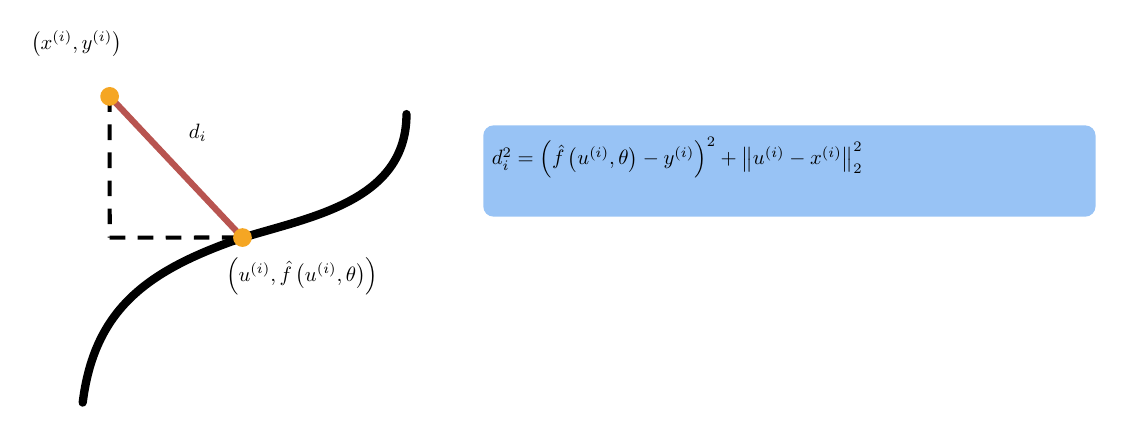
\begin{tikzpicture}[x=0.75pt,y=0.75pt,yscale=-1,xscale=1]
%uncomment if require: \path (0,300); %set diagram left start at 0, and has height of 300

%Shape: Free Drawing [id:dp5002881259079404] 
\draw  [color={rgb, 255:red, 0; green, 0; blue, 0 }  ][line width=3] [line join = round][line cap = round] (63.01,245.57) .. controls (68.41,202.42) and (91.96,183.67) .. (133.01,168.57) .. controls (164.12,157.14) and (219.01,152.23) .. (219.01,106.57) ;
%Straight Lines [id:da19530315633268636] 
\draw [color={rgb, 255:red, 184; green, 84; blue, 80 }  ,draw opacity=1 ][line width=2.25]    (75.99,98.05) -- (139.99,166.05) ;
%Straight Lines [id:da6781226747978477] 
\draw [line width=1.5]  [dash pattern={on 5.63pt off 4.5pt}]  (75.99,98.05) -- (76.01,166.1) ;
%Straight Lines [id:da3955370838358767] 
\draw [line width=1.5]  [dash pattern={on 5.63pt off 4.5pt}]  (76.01,166.1) -- (139.99,166.05) ;
%Shape: Circle [id:dp03457846112388152] 
\draw  [color={rgb, 255:red, 245; green, 166; blue, 35 }  ,draw opacity=1 ][fill={rgb, 255:red, 245; green, 166; blue, 35 }  ,fill opacity=1 ] (135.98,166.05) .. controls (135.98,163.84) and (137.77,162.04) .. (139.99,162.04) .. controls (142.2,162.04) and (144,163.84) .. (144,166.05) .. controls (144,168.27) and (142.2,170.06) .. (139.99,170.06) .. controls (137.77,170.06) and (135.98,168.27) .. (135.98,166.05) -- cycle ;
%Shape: Circle [id:dp15280043442217006] 
\draw  [color={rgb, 255:red, 245; green, 166; blue, 35 }  ,draw opacity=1 ][fill={rgb, 255:red, 245; green, 166; blue, 35 }  ,fill opacity=1 ] (71.98,98.05) .. controls (71.98,95.84) and (73.77,94.04) .. (75.99,94.04) .. controls (78.2,94.04) and (80,95.84) .. (80,98.05) .. controls (80,100.27) and (78.2,102.06) .. (75.99,102.06) .. controls (73.77,102.06) and (71.98,100.27) .. (71.98,98.05) -- cycle ;

% Text Node
\draw (37,65.44) node [anchor=north west][inner sep=0.75pt]  [xscale=0.75,yscale=0.75]  {$\left( x^{( i)} ,y^{( i)}\right)$};
% Text Node
\draw (113,110.4) node [anchor=north west][inner sep=0.75pt]  [xscale=0.75,yscale=0.75]  {$d_{i}$};
% Text Node
\draw  [color={rgb, 255:red, 0; green, 0; blue, 0 }  ,draw opacity=0 ][fill={rgb, 255:red, 152; green, 195; blue, 245 }  ,fill opacity=1 ]  (256,117) .. controls (256,114.24) and (258.24,112) .. (261,112) -- (546,112) .. controls (548.76,112) and (551,114.24) .. (551,117) -- (551,151) .. controls (551,153.76) and (548.76,156) .. (546,156) -- (261,156) .. controls (258.24,156) and (256,153.76) .. (256,151) -- cycle  ;
\draw (259,116.4) node [anchor=north west][inner sep=0.75pt]  [xscale=0.75,yscale=0.75]  {$d_{i}^{2} =\left(\hat{f}\left( u^{(i)} ,\theta \right) -y^{(i)}\right)^{2} +\left\Vert u^{(i)} -x^{(i)}\right\Vert _{2}^{2}$};
% Text Node
\draw (131,174.4) node [anchor=north west][inner sep=0.75pt]  [xscale=0.75,yscale=0.75]  {$\left( u^{(i)} ,\hat{f}\left( u^{(i)} ,\theta \right)\right)$};


\end{tikzpicture}
\end{FigureCenter}

通过 $ u^{(i)} $ 与图中点 $ \left(x^{(i)}, y^{(i)}\right) $ 的平方距离来最小化 $ d_{i}^{2} $.最小化 $ \sum_{i} d_{i}^{2} $ ,即通过 $ u^{(1)}, \ldots, u^{(N)} $ 和 $ \theta $ 来最小化均方距离。

\subsection{二分类}

二分类的目标函数为 $ \hat{f}(x, \theta)=\operatorname{sign}\left(\theta_{1} f_{1}(x)+\theta_{2} f_{2}(x)+\cdots+\theta_{p} f_{p}(x)\right) $ 


\begin{problem}[二分类问题]
    \begin{equation}
\min _{\theta} \sum_{i=1}^{N}\left(\phi\left(\theta_{1} f_{1}\left(x^{(i)}\right)+\cdots+\theta_{p} f_{p}\left(x^{(i)}\right)\right)-y^{(i)}\right)^{2}
\end{equation}

$ \left(x^{(i)}, y^{(i)}\right) $ 是数据点, $ y^{(i)} \in\{-1,1\} $ . $ \phi(u) $ 是sigmoid函数,它是 $\operatorname{sign} (u) $ 函数的一个可微的近似函数。
\begin{equation}
\phi(u)=\frac{e^{u}-e^{-u}}{e^{u}+e^{-u}}
\end{equation}
\end{problem}


通过计算 $ \theta $ 来求解非线性最小二乘问题,\textbf{大概率}能得到良好的结果。



\section{梯度}

\subsection{Gradient and Directional Derivative}

\begin{definition}[$\mathfrak{R}^{n} \rightarrow \mathfrak{R}$函数$g$的梯度]
    可微函数 $ g: \mathfrak{R}^{n} \rightarrow \mathfrak{R} $ 在 $ z \in \mathfrak{R}^{n} $ 的梯度(gradient)为

\begin{equation}
\nabla g(z)=\left[\begin{array}{c}
\frac{\partial g}{\partial x_{1}}(z) \\
\frac{\partial g}{\partial x_{2}}(z) \\
\cdots \\
\frac{\partial g}{\partial x_{n}}(z)
\end{array}\right]
\end{equation}
\end{definition}

\begin{definition}[$g$在$z$附近的仿射近似(一阶泰勒公式,线性化)]
    \begin{equation} \begin{aligned} \hat{g}(x) &=g(z)+\frac{\partial g}{\partial x_{1}}(z)\left(x_{1}-z_{1}\right)+\cdots+\frac{\partial g}{\partial x_{n}}(z)\left(x_{n}-z_{n}\right) \\ &=g(z)+\nabla g(z)^{T}(x-z) \end{aligned} \end{equation}
\end{definition}

\begin{definition}[Directional Derivative]
    For given $ z $ and nonzero $ v $, define $ h(t)=g(z+t v) $

   The derivative of $ h $ at $ t=0 $
\begin{equation}
\begin{aligned}
h^{\prime}(0) &=\frac{\partial g}{\partial x_{1}}(z) v_{1}+\frac{\partial g}{\partial x_{2}}(z) v_{2}+\cdots+\frac{\partial g}{\partial x_{n}}(z) v_{n} \\
&=\nabla g(z)^{T} v
\end{aligned}
\end{equation}

This is called the \term{directional derivative} of $ g $ (at $ z $, in the direction $ v $ ), $ v $ is a \term{descent direction} of $ g $ at $ z $ if $ \nabla g(z)^{T} v<0 $.
\end{definition}

\subsection{Jacobian Matrices}


\begin{definition}[Jacobian Matrices]
    可微函数 $ f: \mathfrak{R}^{n} \rightarrow \mathfrak{R}^{m} $ 在 $ z \in \mathfrak{R}^{n} $ 的导数矩阵(Jacobian矩阵)

\begin{equation}
f(x)=\left[\begin{array}{c}
f_{1}(x) \\
f_{2}(x) \\
\vdots \\
f_{m}(x)
\end{array}\right] \quad D f(z)=\left[\begin{array}{cccc}
\frac{\partial f_{1}}{\partial x_{1}}(z) & \frac{\partial f_{1}}{\partial x_{2}}(z) & \cdots & \frac{\partial f_{1}}{\partial x_{n}}(z) \\
\frac{\partial f_{2}}{\partial x_{1}}(z) & \frac{\partial f_{2}}{\partial x_{2}}(z) & \cdots & \frac{\partial f_{2}}{\partial x_{n}}(z) \\
\vdots & \vdots & & \vdots \\
\frac{\partial f_{m}}{\partial x_{1}}(z) & \frac{\partial f_{m}}{\partial x_{2}}(z) & \cdots & \frac{\partial f_{m}}{\partial x_{n}}(z)
\end{array}\right]
\end{equation}
\end{definition}

\begin{definition}[$ f $ 在 $ z $ 附近的仿射近似(线性化)]
    \begin{equation}\begin{aligned}
        \hat{f} (x) & =f(z)+Df(z)(x-z)\\
         & =\left[\begin{array}{ c }
        f_{1} (z)\\
        f_{2} (z)\\
        \vdots \\
        f_{m} (z)
        \end{array}\right] \ +\left(\left[\begin{array}{ c c c c }
        \textcolor[rgb]{0.72,0.33,0.31}{\frac{\partial f_{1}}{\partial x_{1}} (z)} & \textcolor[rgb]{0.72,0.33,0.31}{\frac{\partial f_{1}}{\partial x_{2}} (z)} & \textcolor[rgb]{0.72,0.33,0.31}{\cdots } & \textcolor[rgb]{0.72,0.33,0.31}{\frac{\partial f_{1}}{\partial x_{n}} (z)}\\
        \frac{\partial f_{2}}{\partial x_{1}} (z) & \frac{\partial f_{2}}{\partial x_{2}} (z) & \cdots  & \frac{\partial f_{2}}{\partial x_{n}} (z)\\
        \vdots  & \vdots  &  & \vdots \\
        \frac{\partial f_{m}}{\partial x_{1}} (z) & \frac{\partial f_{m}}{\partial x_{2}} (z) & \cdots  & \frac{\partial f_{m}}{\partial x_{n}} (z)
        \end{array}\right]\left[\begin{array}{ c }
        \textcolor[rgb]{0.72,0.33,0.31}{x_{1} -z_{1}}\\
        \textcolor[rgb]{0.72,0.33,0.31}{x_{2} -z_{2}}\\
        \textcolor[rgb]{0.72,0.33,0.31}{\vdots }\\
        \textcolor[rgb]{0.72,0.33,0.31}{x_{n} -z_{n}}
        \end{array}\right]\right)_{m\times 1}
        \end{aligned}\end{equation}

    用符号 $ \hat{f}(x ; z) $ 表示点 $ z $ 附近的线性化逼近。
\end{definition}

\subsection{Hessian}

\begin{definition}[Hessian Matrices]
    Hessian of $ g $ at $ z $ is a symmetric $ n \times n $ matrix $ \nabla^{2} g(z) $ with elements
\begin{equation}
\nabla^{2} g(z)_{i j}=\frac{\partial^{2} g}{\partial x_{i} \partial x_{j}}(z)
\end{equation}

This is also the derivative matrix $ D f(z) $ of $ f(x)=\nabla g(x) $ at $ z $.
\end{definition}

\begin{definition}[Quadratic (second order) approximation of $g$ around $z$]
    \begin{equation} g_{{q}}(x)=g(z)+\nabla g(z)^{T}(x-z)+\frac{1}{2}(x-z)^{T} \nabla^{2} g(z)(x-z) \end{equation}
\end{definition}

\begin{example}
    Affine function: $ g(x)=a^{T} x+b $
\begin{equation}
\nabla g(x)=a, \quad \nabla^{2} g(x)=0
\end{equation}

Quadratic function: $ g(x)=x^{T} P x+q^{T} x+r $ with $ P $ symmetric
\begin{equation}
\nabla g(x)=2 P x+q, \quad \nabla^{2} g(x)=2 P
\end{equation}

Least squares cost: $ g(x)=\|A x-b\|^{2}=x^{T} A^{T} A x-2 b^{T} A x+b^{T} b $
\begin{equation}
\nabla g(x)=2 A^{T} A x-2 A^{T} b, \quad \nabla^{2} g(x)=2 A^{T} A
\end{equation}
\end{example}

\begin{theorem}[Linear combination properties]
    If $ g(x)=\alpha_{1} g_{1}(x)+\alpha_{2} g_{2}(x) $, then
\begin{equation}
\begin{aligned}
\nabla g(x) &=\alpha_{1} \nabla g_{1}(x)+\alpha_{2} \nabla g_{2}(x) \\
\nabla^{2} g(x) &=\alpha_{1} \nabla^{2} g_{1}(x)+\alpha_{2} \nabla^{2} g_{2}(x)
\end{aligned}
\end{equation}
\end{theorem}

\begin{theorem}[Composition with affine mapping properties]
    if $ g(x)=h(C x+d) $, then
\begin{equation}
\begin{aligned}
\nabla g(x) &=C^{T} \nabla h(C x+d) \\
\nabla^{2} g(x) &=C^{T} \nabla^{2} h(C x+d) C
\end{aligned}
\end{equation}
\end{theorem}

\begin{example}
    \begin{equation} g\left(x_{1}, x_{2}\right)=e^{x_{1}+x_{2}-1}+e^{x_{1}-x_{2}-1}+e^{-x_{1}-1} \end{equation}

    Gradient
\begin{equation}
\nabla g(x)=\left[\begin{array}{c}
e^{x_{1}+x_{2}-1}+e^{x_{1}-x_{2}-1}-e^{-x_{1}-1} \\
e^{x_{1}+x_{2}-1}-e^{x_{1}-x_{2}-1}
\end{array}\right]
\end{equation}

Hessian
\begin{equation}
\nabla^{2} g(x)=\left[\begin{array}{cc}
e^{x_{1}+x_{2}-1}+e^{x_{1}-x_{2}-1}+e^{-x_{1}-1} & e^{x_{1}+x_{2}-1}-e^{x_{1}-x_{2}-1} \\
e^{x_{1}+x_{2}-1}-e^{x_{1}-x_{2}-1} & e^{x_{1}+x_{2}-1}+e^{x_{1}-x_{2}-1}
\end{array}\right]
\end{equation}

Gradient and Hessian via composition property:

express $ g $ as $ g(x)=h(C x+d) $ with $ h\left(y_{1}, y_{2}, y_{3}\right)=e^{y_{1}}+e^{y_{2}}+e^{y_{3}} $ and
\begin{equation}
C=\left[\begin{array}{rr}
1 & 1 \\
1 & -1 \\
-1 & 0
\end{array}\right], \quad d=\left[\begin{array}{l}
-1 \\
-1 \\
-1
\end{array}\right]
\end{equation}

Gradient: $ \nabla g(x)=C^{T} \nabla h(C x+d) $
\begin{equation}
\nabla g(x)=\left[\begin{array}{rrr}
1 & 1 & -1 \\
1 & -1 & 0
\end{array}\right]\left[\begin{array}{c}
e^{x_{1}+x_{2}-1} \\
e^{x_{1}-x_{2}-1} \\
e^{-x_{1}-1}
\end{array}\right]
\end{equation}

Hessian: $ \nabla^{2} g(x)=C^{T} \nabla h^{2}(C x+d) C $
\begin{equation}
\nabla^{2} g(x)=\left[\begin{array}{rrr}
1 & 1 & -1 \\
1 & -1 & 0
\end{array}\right]\left[\begin{array}{ccc}
e^{x_{1}+x_{2}-1} & 0 & 0 \\
0 & e^{x_{1}-x_{2}-1} & 0 \\
0 & 0 & e^{-x_{1}-1}
\end{array}\right]\left[\begin{array}{rr}
1 & 1 \\
1 & -1 \\
-1 & 0
\end{array}\right]
\end{equation}
\end{example}

\subsection{Optimality conditions for twice differentiable $ g $}

\begin{theorem}[Necessary condition for twice differentiable $ g $]
    If $ x^{\star} $ is locally optimal, then
$ \nabla g\left(x^{\star}\right)=0 $ and $ \nabla^{2} g\left(x^{\star}\right) $ is positive semidefinite
\end{theorem}

\begin{theorem}[Sufficient condition]
    If $ x^{\star} $ satisfies
$ \nabla g\left(x^{\star}\right)=0 $ and $ \nabla^{2} g\left(x^{\star}\right) $ is positive definite
then $ x^{\star} $ is locally optimal.
\end{theorem}

\begin{definition}[Convex functions]
    $ g $ is called \textit{convex} if $ \nabla^{2} g(x) $ is positive semidefinite everywhere.
\end{definition}

\begin{theorem}[Necessary and sufficient condition for convex functions]
    if $ g $ is convex then $ x^{\star} $ is optimal if and only if $ \nabla g\left(x^{\star}\right)=0 $
\end{theorem}




\begin{example}
    $ g(x)=\log \left(e^{x}+e^{-x}\right) $
\begin{equation}
g^{\prime}(x)=\frac{e^{x}-e^{-x}}{e^{x}+e^{-x}}, \quad g^{\prime \prime}(x)=\frac{4}{\left(e^{x}+e^{-x}\right)^{2}}
\end{equation}
$ g^{\prime \prime}(x) \geq 0 $ everywhere; $ x^{\star}=0 $ is the unique optimal point
\end{example}

\begin{example}
    - $ g(x)=x^{4} $
\begin{equation}
g^{\prime}(x)=4 x^{3}, \quad g^{\prime \prime}(x)=12 x^{2}
\end{equation}
$ g^{\prime \prime}(x) \geq 0 $ everywhere; $ x^{\star}=0 $ is the unique optimal point
\end{example}

\begin{example}
    - $ g(x)=x^{3} $
\begin{equation}
g^{\prime}(x)=3 x^{2}, \quad g^{\prime \prime}(x)=6 x
\end{equation}
$ g^{\prime}(0)=0, g^{\prime \prime}(0)=0 $ but $ x=0 $ is not locally optimal
\end{example}

\begin{example}
    - $ g(x)=x^{T} P x+q^{T} x+r $ (P is symmetric positive definite)
\begin{equation}
\nabla g(x)=2 P x+q, \quad \nabla^{2} g(x)=2 P
\end{equation}
$ \nabla^{2} g(x) $ is positive definite everywhere, hence the unique optimal point is
\begin{equation}
x^{\star}=-(1 / 2) P^{-1} q
\end{equation}
\end{example}

\begin{example}
    - $ g(x)=\|A x-b\|^{2} $ ( $ A $ is a matrix with linearly independent columns)
\begin{equation}
\nabla g(x)=2 A^{T} A x-2 A^{T} b, \quad \nabla^{2} g(x)=2 A^{T} A
\end{equation}
$ \nabla^{2} g(x) $ is positive definite everywhere, hence the unique optimal point is
\begin{equation}
x^{\star}=\left(A^{T} A\right)^{-1} A^{T} b
\end{equation}
\end{example}

\begin{example}
    \begin{equation} g\left(x_{1}, x_{2}\right)=e^{x_{1}+x_{2}-1}+e^{x_{1}-x_{2}-1}+e^{-x_{1}-1} \end{equation}

    Gradient
\begin{equation}
\nabla g(x)=\left[\begin{array}{c}
e^{x_{1}+x_{2}-1}+e^{x_{1}-x_{2}-1}-e^{-x_{1}-1} \\
e^{x_{1}+x_{2}-1}-e^{x_{1}-x_{2}-1}
\end{array}\right]
\end{equation}

Hessian
\begin{equation}
\nabla^{2} g(x)=\left[\begin{array}{cc}
e^{x_{1}+x_{2}-1}+e^{x_{1}-x_{2}-1}+e^{-x_{1}-1} & e^{x_{1}+x_{2}-1}-e^{x_{1}-x_{2}-1} \\
e^{x_{1}+x_{2}-1}-e^{x_{1}-x_{2}-1} & e^{x_{1}+x_{2}-1}+e^{x_{1}-x_{2}-1}
\end{array}\right]
\end{equation}


    We can express $ \nabla^{2} g(x) $ as
\begin{equation}
\nabla^{2} g(x)=\left[\begin{array}{rrr}
1 & 1 & 1 \\
1 & -1 & 0
\end{array}\right]\left[\begin{array}{ccc}
e^{x_{1}+x_{2}-1} & 0 & 0 \\
0 & e^{x_{1}-x_{2}-1} & 0 \\
0 & 0 & e^{-x_{1}-1}
\end{array}\right]\left[\begin{array}{rr}
1 & 1 \\
1 & -1 \\
1 & 0
\end{array}\right]
\end{equation}
this shows that $ \nabla^{2} g(x) $ is positive definite for all $ x $
therefore $ x^{\star} $ is optimal if and only if
\begin{equation}
\nabla g\left(x^{\star}\right)=\left[\begin{array}{c}
e^{x_{1}^{\star}+x_{2}^{\star}-1}+e^{x_{1}^{\star}-x_{2}^{\star}-1}-e^{-x_{1}^{\star}-1} \\
e^{x_{1}^{\star}+x_{2}^{\star}-1}-e^{x_{1}^{\star}-x_{2}^{\star}-1}
\end{array}\right]=0
\end{equation}
two nonlinear equations in two variables
\end{example}


\section{求解非线性最小二乘法:目标梯度}

对于优化问题\ref{pbl:non-linear-least-squares}
\begin{equation} g(x)=\|f(x)\|_{2}^{2}=\sum_{i=1}^{m}\left(f_{i}(x)\right)^{2},f(x)=\left[\begin{array}{c}f_{1}(x) \\ f_{2}(x) \\ \vdots \\ f_{m}(x)\end{array}\right] \end{equation}

$ g $ 对 $ x_{j} $ 的一阶导数为
\begin{equation}\begin{aligned}
    \frac{\partial g}{\partial x_{j}} (z) & =2\sum _{i=1}^{m} f_{i} (z)\frac{\partial f_{i}}{\partial x_{j}} (z)\\
     & =2\left[\frac{\partial f_{\textcolor[rgb]{0.49,0.83,0.13}{1}}}{\partial x_{\textcolor[rgb]{0.29,0.56,0.89}{j}}} (z),\frac{\partial f_{\textcolor[rgb]{0.49,0.83,0.13}{2}}}{\partial x_{\textcolor[rgb]{0.29,0.56,0.89}{j}}} (z),\cdots ,\frac{\partial f_{\textcolor[rgb]{0.49,0.83,0.13}{m}}}{\partial x_{\textcolor[rgb]{0.29,0.56,0.89}{j}}} (z)\right]\left[\begin{array}{ c }
    f_{1} (z)\\
    f_{2} (z)\\
    \vdots \\
    f_{m} (z)
    \end{array}\right]
    \end{aligned}\end{equation}

注意到

\begin{equation}\displaystyle (Df(z))^{T} =\left[\begin{array}{ c c c c }
    \frac{\partial f_{\textcolor[rgb]{0.49,0.83,0.13}{1}}}{\partial x_{\textcolor[rgb]{0.29,0.56,0.89}{1}}} (z) & \frac{\partial f_{\textcolor[rgb]{0.49,0.83,0.13}{2}}}{\partial x_{\textcolor[rgb]{0.29,0.56,0.89}{1}}} (z) & \cdots  & \frac{\partial f_{\textcolor[rgb]{0.49,0.83,0.13}{m}}}{\partial x_{\textcolor[rgb]{0.29,0.56,0.89}{1}}} (z)\\
    \frac{\partial f_{\textcolor[rgb]{0.49,0.83,0.13}{1}}}{\partial x_{\textcolor[rgb]{0.29,0.56,0.89}{2}}} (z) & \frac{\partial f_{\textcolor[rgb]{0.49,0.83,0.13}{2}}}{\partial x_{\textcolor[rgb]{0.29,0.56,0.89}{2}}} (z) & \cdots  & \frac{\partial f_{\textcolor[rgb]{0.49,0.83,0.13}{m}}}{\partial x_{\textcolor[rgb]{0.29,0.56,0.89}{2}}} (z)\\
    \vdots  & \vdots  &  & \vdots \\
    \frac{\partial f_{\textcolor[rgb]{0.49,0.83,0.13}{1}}}{\partial x_{\textcolor[rgb]{0.29,0.56,0.89}{n}}} (z) & \frac{\partial f_{\textcolor[rgb]{0.49,0.83,0.13}{2}}}{\partial x_{\textcolor[rgb]{0.29,0.56,0.89}{n}}} (z) & \cdots  & \frac{\partial f_{\textcolor[rgb]{0.49,0.83,0.13}{m}}}{\partial x_{\textcolor[rgb]{0.29,0.56,0.89}{n}}} (z)
    \end{array}\right] =[ \nabla f_{1} (z),\nabla f_{2} (z),\cdots ,\nabla f_{m} (z)]\end{equation}

    $ g $ 在 $ z $ 的梯度为
    \begin{equation}
    \nabla g(z)=\left[\begin{array}{c}
    \frac{\partial g}{\partial x_{1}}(z) \\
    \vdots \\
    \frac{\partial g}{\partial x_{n}}(z)
    \end{array}\right]=2 \sum_{i=1}^{m} f_{i}(z) \nabla f_{i}(z)=2(D f(z))^{T} f(z)
    \end{equation}

\begin{theorem}[非线性最小二乘问题的最优必要条件]
        \begin{equation}
    \min _{x} g(x)=\sum_{i=1}^{m} f_{i}(x)^{2} \quad f(x)=\left[\begin{array}{c}
    f_{1}(x) \\
    f_{2}(x) \\
    \vdots \\
    f_{m}(x)
    \end{array}\right]
    \end{equation}

    如果要 $ x $ 使 $ g(x) $ 最小,则必须满足:
    \begin{equation}
    \nabla g(x)=2 D f(x)^{T} f(x)=0
    \end{equation}
\end{theorem}

\begin{corollary}[正规方程的最优必要条件]
    推广到正规方程,如果 $ f(x)=A x-b $ ,那么 $ D f(x)=A $ 和
\begin{equation}
\nabla g(x)=2 A^{T}(A x-b)
\end{equation}
\end{corollary}

\begin{remark}
    对于一般函数 $ f(x), \nabla g(x)=0 $ \textbf{不是最优解的充分条件}.
\end{remark}



\section{Gauss-Newton Algorithm}

\begin{problem}
    \begin{equation}
\min _{x} g(x)=\|f(x)\|_{2}^{2}=\sum_{i=1}^{m} f_{i}(x)^{2}
\end{equation}

从某个初始值 $ x^{(1)} $ 开始,当迭代 $ x^{(2)}, x^{(3)}, \ldots $.
\end{problem}

函数 $ f $ 在 $ x^{(k)} $ 附近的泰勒展开式是

\begin{equation}
\hat{f}\left(x ; x^{(k)}\right)=f\left(x^{(k)}\right)+D f\left(x^{(k)}\right)\left(x-x^{(k)}\right)
\end{equation}

用仿射近似 $ \hat{f}\left(x, x^{(k)}\right) $ 代替最小二乘法问题中函数 $ f(x) $

\begin{equation}
x^{(k+1)}=\arg \min _{x}\left\|\hat{f}\left(x ; x^{(k)}\right)\right\|_{2}^{2}
\end{equation}

第$k$次迭代问题:
\begin{equation}
\begin{array}{c}
x^{(k+1)}=\arg \min _{x}\left\|\hat{f}\left(x ; x^{(k)}\right)\right\|_{2}^{2} \\
x^{(k+1)}=\arg \min _{x} h(x)=\left\|f\left(x^{(k)}\right)+D f\left(x^{(k)}\right)\left(x-x^{(k)}\right)\right\|_{2}^{2}
\end{array}
\end{equation}

函数 $ h(x) $ 的梯度:
\begin{equation}
\nabla h(x)=2 D f\left(x^{(k)}\right)^{T}\left(f\left(x^{(k)}\right)+D f\left(x^{(k)}\right)\left(x-x^{(k)}\right)\right)=0
\end{equation}

则有
\begin{equation} D f\left(x^{(k)}\right)^{T} D f\left(x^{(k)}\right) x^{(k)}-D f\left(x^{(k)}\right)^{T} f\left(x^{(k)}\right)=D f\left(x^{(k)}\right)^{T} D f\left(x^{(k)}\right) x \end{equation}

\begin{equation} D f\left(x^{(k)}\right)^{T} D f\left(x^{(k)}\right) x^{(k)}-D f\left(x^{(k)}\right)^{T} f\left(x^{(k)}\right)=D f\left(x^{(k)}\right)^{T} D f\left(x^{(k)}\right) x \end{equation}

如果 $ D f\left(x^{(k)}\right) $ 的列是线性无关的,则其解为:
\begin{equation}
x^{(k+1)}=x^{(k)}-\left(D f\left(x^{(k)}\right)^{T} D f\left(x^{(k)}\right)\right)^{-1} D f\left(x^{(k)}\right)^{T} f\left(x^{(k)}\right)
\end{equation}

高斯-牛顿法步骤 $ \Delta x^{(k)}=x^{(k+1)}-x^{(k)} $ :
\begin{equation}
\begin{aligned}
\Delta x^{(k)} &=-\left(D f\left(x^{(k)}\right)^{T} D f\left(x^{(k)}\right)\right)^{-1} D f\left(x^{(k)}\right)^{T} f\left(x^{(k)}\right) \\
&=-\frac{1}{2}\left(D f\left(x^{(k)}\right)^{T} D f\left(x^{(k)}\right)\right)^{-1} \nabla g\left(x^{(k)}\right)
\end{aligned}
\end{equation}

(利用第14.10的 $ \nabla g(x) $ 表达式).

逼近函数 $ \hat{f}\left(x ; x^{(k)}\right) $ 的关于 $ x^{(k+1)} $ 的代价:
\begin{equation}
\begin{aligned}
\|\left.\hat{f}\left(x^{(k+1)} ; x^{(k)}\right)\right|_{2} ^{2} &=\| f\left(x^{(k)}\right)+D f\left(x^{(k)}\right) \Delta x^{(k)}||_{2}^{2} \\
&=\left\|\left.f\left(x^{(k)}\right)\right|_{2} ^{2}+2 f\left(x^{(k)}\right)^{T} D f\left(x^{(k)}\right) \Delta x^{(k)}+\right\| D f\left(x^{(k)}\right) \Delta x^{(k)} \|_{2}^{2}
\end{aligned}
\end{equation}

\begin{equation}\begin{aligned}
    & 2Df\left( x^{(k)}\right)^{T}\left( f\left( x^{(k)}\right) +Df\left( x^{(k)}\right)\left( x^{(k+1)} -x^{(k)}\right)\right) =0\quad ( 目标梯度等于0)\\
   \Rightarrow  & Df\left( x^{(k)}\right)^{T} f\left( x^{(k)}\right) =-Df\left( x^{(k)}\right)^{T} Df\left( x^{(k)}\right) \Delta x^{(k)}\\
   \Rightarrow  & \left( \Delta x^{(k)}\right)^{T} Df\left( x^{(k)}\right)^{T} f\left( x^{(k)}\right) =-\left( \Delta x^{(k)}\right)^{T} Df\left( x^{(k)}\right)^{T} Df\left( x^{(k)}\right) \Delta x^{(k)} =-\left\Vert Df\left( x^{(k)}\right) \Delta x^{(k)}\right\Vert _{2}^{2}
   \end{aligned}\end{equation}

\begin{equation} \left\|\hat{f}\left(x^{(k+1)} ; x^{(k)}\right)\right\|_{2}^{2}=\left\|f\left(x^{(k)}\right)\right\|_{2}^{2}-\left\|D f\left(x^{(k)}\right) \Delta x^{(k)}\right\|_{2}^{2} \end{equation}

如果 $ D f\left(x^{(k)}\right) $ 的列向量线性无关,且 $ \Delta x^{(k)} \neq 0 $ :

\begin{equation} \left\|D f\left(x^{(k)}\right) \Delta x^{(k)}\right\|_{2}^{2}>0 \Rightarrow\left\|\hat{f}\left(x^{(k+1)} ; x^{(k)}\right)\right\|_{2}^{2}<\left\|f\left(x^{(k)}\right)\right\|_{2}^{2} \end{equation}

当 $ {m}={n} $ 时, $ D f\left(x^{(k)}\right) $ 的列向量线性无关,高斯-牛顿法可简化为

\begin{equation}
\begin{aligned}
x^{(k+1)} &=x^{(k)}-\left(D f\left(x^{(k)}\right)^{T} D f\left(x^{(k)}\right)\right)^{-1} D f\left(x^{(k)}\right)^{T} f\left(x^{(k)}\right) \\
&=x^{(k)}-\left(D f\left(x^{(k)}\right)\right)^{-1}\left(D f\left(x^{(k)}\right)^{T}\right)^{-1} D f\left(x^{(k)}\right)^{T} f\left(x^{(k)}\right) \\
&=x^{(k)}-\left(D f\left(x^{(k)}\right)\right)^{-1} f\left(x^{(k)}\right) .
\end{aligned}
\end{equation}


如果 $ m=n=1 $ 时,迭代更新可进一步简化为

\begin{equation} x^{(k+1)}=x^{(k)}-\frac{f\left(x^{(k)}\right)}{f^{\prime}\left(x^{(k)}\right)}, f^{\prime}\left(x^{(k)}\right) \neq 0 \end{equation}

\begin{FigureCenter}{$m=n=1$时的情形}

\tikzset{every picture/.style={line width=0.75pt}} %set default line width to 0.75pt        

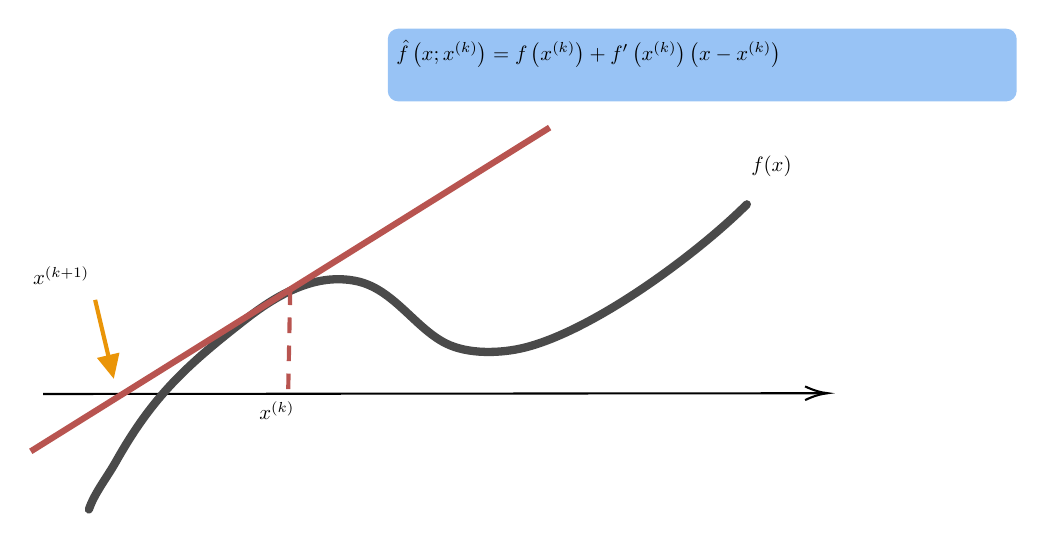
\begin{tikzpicture}[x=0.75pt,y=0.75pt,yscale=-1,xscale=1]
%uncomment if require: \path (0,300); %set diagram left start at 0, and has height of 300

%Straight Lines [id:da987456347938684] 
\draw    (77,220) -- (453,219.62) ;
\draw [shift={(455,219.62)}, rotate = 179.94] [color={rgb, 255:red, 0; green, 0; blue, 0 }  ][line width=0.75]    (10.93,-3.29) .. controls (6.95,-1.4) and (3.31,-0.3) .. (0,0) .. controls (3.31,0.3) and (6.95,1.4) .. (10.93,3.29)   ;
%Shape: Free Drawing [id:dp3634235085264048] 
\draw  [color={rgb, 255:red, 74; green, 74; blue, 74 }  ,draw opacity=1 ][line width=3] [line join = round][line cap = round] (99,275.62) .. controls (101.57,267.9) and (107.73,260.2) .. (112,252.62) .. controls (129.65,221.23) and (145.74,206.38) .. (175,183.62) .. controls (189.89,172.03) and (208.34,161.45) .. (228,165.62) .. controls (245.71,169.37) and (256.02,188.13) .. (271,195.62) .. controls (281.7,200.97) and (297.45,200.51) .. (309,197.62) .. controls (342.7,189.19) and (392.52,152.1) .. (416,128.62) ;
%Straight Lines [id:da8212140101743735] 
\draw [color={rgb, 255:red, 184; green, 84; blue, 80 }  ,draw opacity=1 ][line width=1.5]  [dash pattern={on 5.63pt off 4.5pt}]  (196,169.62) -- (195,219.62) ;
%Straight Lines [id:da6887048674569021] 
\draw [color={rgb, 255:red, 184; green, 84; blue, 80 }  ,draw opacity=1 ][line width=2.25]    (196,169.62) -- (321,91.62) ;
%Straight Lines [id:da06334358045468957] 
\draw [color={rgb, 255:red, 184; green, 84; blue, 80 }  ,draw opacity=1 ][line width=2.25]    (71,247.62) -- (196,169.62) ;
%Straight Lines [id:da7554536985475104] 
\draw [color={rgb, 255:red, 234; green, 149; blue, 8 }  ,draw opacity=1 ][fill={rgb, 255:red, 184; green, 84; blue, 80 }  ,fill opacity=1 ][line width=1.5]    (102,174.65) -- (110.06,208.73) ;
\draw [shift={(110.98,212.62)}, rotate = 256.69] [fill={rgb, 255:red, 234; green, 149; blue, 8 }  ,fill opacity=1 ][line width=0.08]  [draw opacity=0] (11.61,-5.58) -- (0,0) -- (11.61,5.58) -- cycle    ;

% Text Node
\draw (180,222.4) node [anchor=north west][inner sep=0.75pt]  [xscale=0.75,yscale=0.75]  {$x^{( k)}$};
% Text Node
\draw (71,157.4) node [anchor=north west][inner sep=0.75pt]  [xscale=0.75,yscale=0.75]  {$x^{( k+1)}$};
% Text Node
\draw (417,104.4) node [anchor=north west][inner sep=0.75pt]  [xscale=0.75,yscale=0.75]  {$f( x)$};
% Text Node
\draw  [color={rgb, 255:red, 0; green, 0; blue, 0 }  ,draw opacity=0 ][fill={rgb, 255:red, 152; green, 195; blue, 245 }  ,fill opacity=1 ]  (243,49) .. controls (243,46.24) and (245.24,44) .. (248,44) -- (541,44) .. controls (543.76,44) and (546,46.24) .. (546,49) -- (546,74) .. controls (546,76.76) and (543.76,79) .. (541,79) -- (248,79) .. controls (245.24,79) and (243,76.76) .. (243,74) -- cycle  ;
\draw (246,48.4) node [anchor=north west][inner sep=0.75pt]  [xscale=0.75,yscale=0.75]  {$\hat{f}\left( x;x^{(k)}\right) =f\left( x^{(k)}\right) +f^{\prime }\left( x^{(k)}\right)\left( x-x^{(k)}\right)$};


\end{tikzpicture}
\end{FigureCenter}

\subsection{高斯-牛顿法的问题}

然而, $ \hat{f}\left(x ; x^{(k)}\right) $ 只是 $ f(x) $ 的局部近似,仍然可能会有

\begin{remark}
    存在
\begin{equation}
\left\|f\left(x^{(k+1)}\right)\right\|_{2}^{2}>\left\|f\left(x^{(k)}\right)\right\|_{2}^{2}
\end{equation}

的情况。
\end{remark}


Jacobian矩阵Df $ \left(x^{(k)}\right) $ 的可能 "列向量是线性相关。

\begin{remark}
    此时$ \left(D f\left(x^{(k)}\right)^{T} D f\left(x^{(k)}\right)\right) $ 奇异,不可逆。
\end{remark}



\section{Levenberg-Marquardt Algorithm}

Levenberg-Marquardt(LM)算法解决高斯-牛顿法的两个难点:

\begin{enumerate}
    \item 当列 $ D f\left(x^{(k)}\right) $ 是线性相关时,如何更新 $ x^{(k)} $ ?
    \item 当高斯-牛顿法的更新过程, $ \|f(x)\|_{2}^{2} $ 并没有减少。
\end{enumerate}

\subsection{推导Levenberg-Marquardt算法}

LM算法通过求解正则化最小二乘法更新 $ x^{(k+1)} $ :

\begin{problem}
    \begin{equation}
    x^{(k+1)}=\arg \min _{x}\left\|\hat{f}\left(x ; x^{(k)}\right)\right\|_{2}^{2}+\lambda^{(k)}\left\|x-x^{(k)}\right\|_{2}^{2}
    \end{equation}

要求 $ x $ 靠近 $ x^{(k)} $ ,即 $ \hat{f}\left(x ; x^{(k)}\right) \approx f(x) $. (The second term forces $ x $ to be close to $ x^{(k)} $ where $ \hat{f}\left(x ; x^{(k)}\right) \approx f(x) $.)
\end{problem}

当 $ \lambda^{(k)}>0 $ 时,总有唯一解。

\begin{remark}
    Levenberg-Marquardt Algorithm无需再对 $Df \left(x^{(k)}\right) $ 限制。
\end{remark}

\begin{problem}
    第 $ k $ 次迭代求解的最小二乘正则化问题:
\begin{equation}
x^{(k+1)}=\arg \min _{x}\left\|f\left(x^{(k)}\right)+D f\left(x^{(k)}\right)\left(x-x^{(k)}\right)\right\|_{2}^{2}+\lambda^{(k)}\left\|x-x^{(k)}\right\|_{2}^{2}
\end{equation}
\end{problem}



令目标函数导数等于 0 :
\begin{equation}
\begin{aligned}
    & 2Df\left( x^{(k)}\right)^{T}\left( f\left( x^{(k)}\right) +Df\left( x^{(k)}\right)\left( x-x^{(k)}\right)\right) +2\lambda ^{(k)}\left( x-x^{(k)}\right) =0\\
   \Rightarrow  & \left( Df\left( x^{(k)}\right)^{T} Df\left( x^{(k)}\right) +\lambda ^{(k)} I\right)\left( x-x^{(k)}\right) =-Df\left( x^{(k)}\right)^{T} f\left( x^{(k)}\right)
   \end{aligned}
\end{equation}

$ x^{(k+1)} $ 更新:
\begin{equation}
x^{(k+1)}=x^{(k)}-\left(D f\left(x^{(k)}\right)^{T} D f\left(x^{(k)}\right)+\lambda^{(k)} I\right)^{-1} D f\left(x^{(k)}\right)^{T} f\left(x^{(k)}\right)
\end{equation}

\begin{theorem}
    LM算法步骤 $ \Delta x^{(k)}=x^{(k+1)}-x^{(k)} $ 是:

\begin{equation} \begin{aligned} \Delta x^{(k)} &=-\left(D f\left(x^{(k)}\right)^{T} D f\left(x^{(k)}\right)+\lambda^{(k)} I\right)^{-1} D f\left(x^{(k)}\right)^{T} f\left(x^{(k)}\right) \\ &=-\frac{1}{2}\left(D f\left(x^{(k)}\right)^{T} D f\left(x^{(k)}\right)+\lambda^{(k)} I\right)^{-1} \nabla g\left(x^{(k)}\right) \end{aligned} \end{equation}
\end{theorem}

\begin{theorem}
    对于 $ \lambda^{(k)}=0 $ ,简化为高斯-牛顿法
\end{theorem}

\begin{theorem}
    对于较大的 $ \lambda^{(k)} $ :
\begin{equation}
\Delta x^{(k)} \approx-\frac{1}{2 \lambda^{(k)}} \nabla g\left(x^{(k)}\right)
\end{equation}
\end{theorem}



\subsection{正则化参数}

几种调整 $ \lambda^{(k)} $ 的策略。

\begin{algorithm}[htbp]
    \caption{在第$k$次迭代时,求解$\hat{x}$}
    $
    \hat{x}=\arg \min _{x}\left\|\hat{f}\left(x ; x^{(k)}\right)\right\|_{2}^{2}+\lambda^{(k)}\left\|x-x^{(k)}\right\|_{2}^{2}
    $\;
    

    \If(){$ \|f(\hat{x})\|_{2}^{2}<\left\|f\left(x^{(k)}\right)\right\|_{2}^{2} $}{
        $ x^{(k+1)}=\hat{x} $\;
        降低 $ \lambda $
    }
    \Else(){
        无需更新 $ x \left(x^{(k+1)}=x^{(k)}\right) $\;
        增加 $ \lambda $\;

    }
\end{algorithm}

它的一些变化:

\begin{example}
    比较预期损失降低的情况和实际损失降低的情况。(compare actual cost reduction with predicted cost reduction)
\end{example}

\begin{theorem}
    在第$k$次迭代时,求解$\hat{x}$

    \begin{equation}
    \hat{x}=\arg \min _{x}\left\|\hat{f}\left(x ; x^{(k)}\right)\right\|_{2}^{2}+\lambda^{(k)}\left\|x-x^{(k)}\right\|_{2}^{2}
    \end{equation}

    等价于

    具有“置信区间”的最小二乘法问题:
    $ \min _{x}\left\|\hat{f}\left(x ; x^{(k)}\right)\right\|_{2}^{2} $
    subject to $ \left\|x-x^{(k)}\right\|_{2}^{2} \leq \gamma $
\end{theorem}


\begin{algorithm}[htbp]
    \caption{Levenberg-Marquardt Algorithm}
    选择 $ x^{(1)} $ 和 $ \lambda^{(1)} $\;
    \While{$ k=1,2, \ldots $}{
        求 $ f\left(x^{(k)}\right) $\;
        $ A=D f\left(x^{(k)}\right) $\;
        计算最小二乘法正则化问题的解:
        \begin{equation}
        \hat{x}=x^{(k)}-\left(A^{T} A+\lambda^{(k)} I\right)^{-1} A^{T} f\left(x^{(k)}\right)
        \end{equation}\;
        计算 $ x^{(k+1)} $ 和 $ \lambda^{(k+1)} $ :
        \begin{equation}\displaystyle \left\{\begin{array}{ c c c }
        x^{(k+1)} =\hat{x} , & \lambda ^{(k+1)} =\beta _{1} \lambda ^{(k)} & \left(\text{if} \ \| (\hat{x} )\| _{2}^{2} < \left\Vert f\left( x^{(k)}\right)\right\Vert _{2}^{2}\right)\\
        x^{(k+1)} =x^{(k)} , & \lambda ^{(k+1)} =\beta _{2} \lambda ^{(k)} & \left(\text{others}\right)
        \end{array}\right. \end{equation}\;

    }
\end{algorithm}

\begin{itemize}
    \item 其中 $ \beta_{1}, \beta_{2} $ 是常数, $ 0<\beta_{1}<1<\beta_{2} $ .
    \item 在步骤2中,可以使用 $ {QR} $ 分解来计算 $ \hat{x} $ .
    \item 迭代会在当 $ \nabla g\left(x^{(k)}\right)=2 A^{T} f\left(x^{(k)}\right) $ 足够小时终止。
\end{itemize}

\section{Newton Method}

\begin{proposition}
    Assume $ f: \mathfrak{R}^{n} \rightarrow \mathfrak{R}^{n} $ is differentiable.
\end{proposition}



\begin{algorithm}
    \caption{Newton's Method}
     choose $ x^{(1)} $\;
     \While{$ k=1,2, \ldots $}{
         \begin{equation}
        x^{(k+1)}=x^{(k)}-D f\left(x^{(k)}\right)^{-1} f\left(x^{(k)}\right)
        \end{equation}\;
     }
\end{algorithm}



$ D f\left(x^{(k)}\right) $ is the derivative matrix of $ f $ at $ x^{(k)} $. 

Each iteration requires one evaluation of $ f(x) $ and $ D f(x) $, each iteration requires factorization of the $ n \times n $ matrix $ D f(x) $.

\begin{proposition}
    We assume $ D f(x) $ is nonsingular.
\end{proposition}

\subsection{Interpretation of Newton Method}

\begin{equation}
x^{(k+1)}=x^{(k)}-D f\left(x^{(k)}\right)^{-1} f\left(x^{(k)}\right)
\end{equation}

linearize $ f $ (i.e., make affine approximation) around current iterate $ x^{(k)} $
\begin{equation}
\hat{f}\left(x ; x^{(k)}\right)=f\left(x^{(k)}\right)+D f\left(x^{(k)}\right)\left(x-x^{(k)}\right)
\end{equation}

solve the linearized equation $ \hat{f}\left(x ; x^{(k)}\right)=0 $; the solution is
\begin{equation}
x=x^{(k)}-D f\left(x^{(k)}\right)^{-1} f\left(x^{(k)}\right)
\end{equation}

take the solution $ x $ of the linearized equation as the next iterate $ x^{(k+1)} $

\subsection{One Variable}

\begin{FigureCenter}{$m=n=1$时的情形}

    \tikzset{every picture/.style={line width=0.75pt}} %set default line width to 0.75pt        
    
    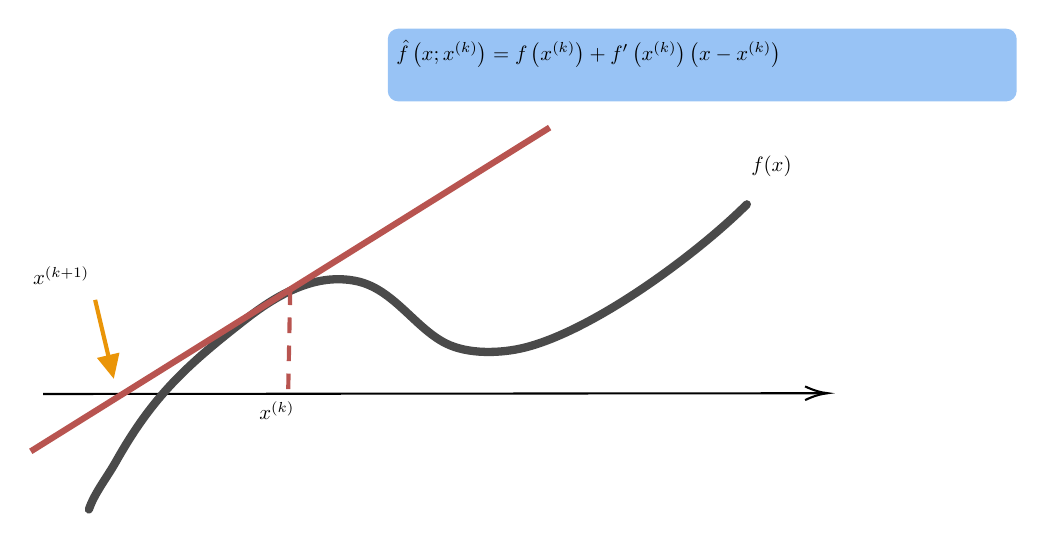
\begin{tikzpicture}[x=0.75pt,y=0.75pt,yscale=-1,xscale=1]
    %uncomment if require: \path (0,300); %set diagram left start at 0, and has height of 300
    
    %Straight Lines [id:da987456347938684] 
    \draw    (77,220) -- (453,219.62) ;
    \draw [shift={(455,219.62)}, rotate = 179.94] [color={rgb, 255:red, 0; green, 0; blue, 0 }  ][line width=0.75]    (10.93,-3.29) .. controls (6.95,-1.4) and (3.31,-0.3) .. (0,0) .. controls (3.31,0.3) and (6.95,1.4) .. (10.93,3.29)   ;
    %Shape: Free Drawing [id:dp3634235085264048] 
    \draw  [color={rgb, 255:red, 74; green, 74; blue, 74 }  ,draw opacity=1 ][line width=3] [line join = round][line cap = round] (99,275.62) .. controls (101.57,267.9) and (107.73,260.2) .. (112,252.62) .. controls (129.65,221.23) and (145.74,206.38) .. (175,183.62) .. controls (189.89,172.03) and (208.34,161.45) .. (228,165.62) .. controls (245.71,169.37) and (256.02,188.13) .. (271,195.62) .. controls (281.7,200.97) and (297.45,200.51) .. (309,197.62) .. controls (342.7,189.19) and (392.52,152.1) .. (416,128.62) ;
    %Straight Lines [id:da8212140101743735] 
    \draw [color={rgb, 255:red, 184; green, 84; blue, 80 }  ,draw opacity=1 ][line width=1.5]  [dash pattern={on 5.63pt off 4.5pt}]  (196,169.62) -- (195,219.62) ;
    %Straight Lines [id:da6887048674569021] 
    \draw [color={rgb, 255:red, 184; green, 84; blue, 80 }  ,draw opacity=1 ][line width=2.25]    (196,169.62) -- (321,91.62) ;
    %Straight Lines [id:da06334358045468957] 
    \draw [color={rgb, 255:red, 184; green, 84; blue, 80 }  ,draw opacity=1 ][line width=2.25]    (71,247.62) -- (196,169.62) ;
    %Straight Lines [id:da7554536985475104] 
    \draw [color={rgb, 255:red, 234; green, 149; blue, 8 }  ,draw opacity=1 ][fill={rgb, 255:red, 184; green, 84; blue, 80 }  ,fill opacity=1 ][line width=1.5]    (102,174.65) -- (110.06,208.73) ;
    \draw [shift={(110.98,212.62)}, rotate = 256.69] [fill={rgb, 255:red, 234; green, 149; blue, 8 }  ,fill opacity=1 ][line width=0.08]  [draw opacity=0] (11.61,-5.58) -- (0,0) -- (11.61,5.58) -- cycle    ;
    
    % Text Node
    \draw (180,222.4) node [anchor=north west][inner sep=0.75pt]  [xscale=0.75,yscale=0.75]  {$x^{( k)}$};
    % Text Node
    \draw (71,157.4) node [anchor=north west][inner sep=0.75pt]  [xscale=0.75,yscale=0.75]  {$x^{( k+1)}$};
    % Text Node
    \draw (417,104.4) node [anchor=north west][inner sep=0.75pt]  [xscale=0.75,yscale=0.75]  {$f( x)$};
    % Text Node
    \draw  [color={rgb, 255:red, 0; green, 0; blue, 0 }  ,draw opacity=0 ][fill={rgb, 255:red, 152; green, 195; blue, 245 }  ,fill opacity=1 ]  (243,49) .. controls (243,46.24) and (245.24,44) .. (248,44) -- (541,44) .. controls (543.76,44) and (546,46.24) .. (546,49) -- (546,74) .. controls (546,76.76) and (543.76,79) .. (541,79) -- (248,79) .. controls (245.24,79) and (243,76.76) .. (243,74) -- cycle  ;
    \draw (246,48.4) node [anchor=north west][inner sep=0.75pt]  [xscale=0.75,yscale=0.75]  {$\hat{f}\left( x;x^{(k)}\right) =f\left( x^{(k)}\right) +f^{\prime }\left( x^{(k)}\right)\left( x-x^{(k)}\right)$};
    
    
    \end{tikzpicture}
    \end{FigureCenter}

affine approximation of $ f $ around $ x^{(k)} $ is
\begin{equation}
\hat{f}\left(x ; x^{(k)}\right)=f\left(x^{(k)}\right)+f^{\prime}\left(x^{(k)}\right)\left(x-x^{(k)}\right)
\end{equation}

solve the linearized equation $ \hat{f}\left(x ; x^{(k)}\right)=0 $ and take the solution as $ x^{(k+1)} $ :
\begin{equation}
x^{(k+1)}=x^{(k)}-\frac{f\left(x^{(k)}\right)}{f^{\prime}\left(x^{(k)}\right)}
\end{equation}

\subsection{Relation to Gauss-Newton method}

recall Gauss-Newton method for nonlinear least squares problem

\begin{problem}[nonlinear least squares problem]
    \begin{equation}\term{minimize} \quad\|f(x)\|^{2} \end{equation}
\end{problem}

where $ f $ is a differentiable function from $ \mathfrak{R}^{n} $ to $ \mathfrak{R}^{m} $.

Gauss-Newton update
\begin{equation}
x^{(k+1)}=x^{(k)}-\left(D f\left(x^{(k)}\right)^{T} D f\left(x^{(k)}\right)\right)^{-1} D f\left(x^{(k)}\right)^{T} f\left(x^{(k)}\right)
\end{equation}

If $ m=n $, then $ D f(x) $ is square and this is the Newton update
\begin{equation}
x^{(k+1)}=x^{(k)}-D f\left(x^{(k)}\right)^{-1} f\left(x^{(k)}\right)
\end{equation}

\subsection{Examples}

\begin{example}
    % todo (2021-12-10 07:54): figure
    \begin{equation} f_{1}\left(x_{1}, x_{2}\right)=\log \left(x_{1}^{2}+2 x_{2}^{2}+1\right)-0.5=0 \end{equation}
\begin{equation} f_{2}\left(x_{1}, x_{2}\right)=x_{2}-x_{1}^{2}+0.2=0 \end{equation}

two equations in two variables; two solutions $ (0.70,0.29),(-0.70,0.29) $.

Newton iteration

\begin{algorithm}[htbp]
    \caption{Newton iteration}
    evaluate $ g=f(x) $ and
\begin{equation}
H=D f(x)=\left[\begin{array}{cc}
2 x_{1} /\left(x_{1}^{2}+2 x_{2}^{2}+1\right) & 4 x_{2} /\left(x_{1}^{2}+2 x_{2}^{2}+1\right) \\
-2 x_{1} & 1
\end{array}\right]
\end{equation}\;
solve $ H v=-g $ (two linear equations in two variables)\;
update $ x:=x+v $\;
\end{algorithm}


Results: 

\begin{itemize}
    \item $ x^{(1)}=(1,1) $ : converges to $ x^{\star}=(0.70,0.29) $ in about 4 iterations
    \item $ x^{(1)}=(-1,1) $ : converges to $ x^{\star}=(-0.70,0.29) $ in about 4 iterations
    \item $ x^{(1)}=(1,-1) $ or $ x^{(0)}=(-1,-1): $ does not converge
\end{itemize}

\end{example}

\begin{itemize}
    \item Newton's method works very well if started near a solution, may not work otherwise
    \item can converge to different solutions depending on the starting point
    \item does not necessarily find the solution closest to the starting point
\end{itemize}

\subsection{Convergence of Newton's method}

Quadratic convergence explains fast convergence when started near solution.

\begin{theorem}[Quadratic Convergence]
    if $ f\left(x^{\star}\right)=0 $ and $ D f\left(x^{\star}\right) $ is nonsingular, and $ x^{(1)} $ is sufficiently close to $ x^{\star} $, then
\begin{equation}
x^{(k)} \rightarrow x^{\star}, \quad\left\|x^{(k+1)}-x^{\star}\right\| \leq c\left\|x^{(k)}-x^{\star}\right\|^{2}
\end{equation}
for some $ c>0 $
\end{theorem}

\subsection{Newton's method for minimizing a convex function}

if $ \nabla^{2} g(x) $ is positive definite everywhere, we can minimize $ g(x) $ by solving
\begin{equation}
\nabla g(x)=0
\end{equation}


Algorithm:
\begin{algorithm}[htbp]
    \caption{Newton's method for minimizing a convex function}
    choose $ x^{(1)} $\;
    \While(){$ k=1,2, \ldots $}{
        \begin{equation}
x^{(k+1)}=x^{(k)}-\nabla^{2} g\left(x^{(k)}\right)^{-1} \nabla g\left(x^{(k)}\right)
\end{equation}\;
    }
\end{algorithm}

$ v=-\nabla^{2} g(x)^{-1} \nabla g(x) $ is called the Newton step at $ x $.

It converges if started sufficiently close to the solution. Newton step is computed by a Cholesky factorization of the Hessian.

\subsubsection{Interpretations of Newton step}


\begin{definition}[affine approximation of $ f(x)=\nabla g(x) $ around $ x^{(k)} $]
    \begin{equation}
\hat{f}\left(x ; x^{(k)}\right)=\nabla g\left(x^{(k)}\right)+\nabla^{2} g\left(x^{(k)}\right)\left(x-x^{(k)}\right)
\end{equation}
\end{definition} is

Newton update $ x^{(k+1)} $ is solution of linear equation $ \hat{f}\left(x ; x^{(k)}\right)=0 $.

\begin{definition}[quadratic approximation of $ g(x) $ around $ x^{(k)} $]
    \begin{equation}
g_{{q}}\left(x ; x^{(k)}\right)=g\left(x^{(k)}\right)+\nabla g\left(x^{(k)}\right)^{T}\left(x-x^{(k)}\right)+\frac{1}{2}\left(x-x^{(k)}\right)^{T} \nabla^{2} g\left(x^{(k)}\right)\left(x-x^{(k)}\right)
\end{equation}
\end{definition}

Newton update $ x^{(k+1)} $ minimizes $ g_{{q}}\left(x ; x^{(k)}\right)\left(\right. $ satisfies $ \left.\nabla g_{{q}}\left(x ; x^{(k)}\right)=0\right) $

% todo (2021-12-10 08:48): figure

\subsection{Damped Newton method}

\begin{algorithm}
    \caption{Damped Newton method}
    choose $ x^{(1)} $\;
    \While(){$ k=1,2, \ldots $}{
        compute Newton step $ v=-\nabla^{2} g\left(x^{(k)}\right)^{-1} \nabla g\left(x^{(k)}\right) $\;
        (Line Search) find largest $ t $ in $ \left\{1,0.5,0.5^{2}, 0.5^{3}, \ldots\right\} $ that satisfies
        \begin{equation}
        g\left(x^{(k)}+t v\right)<g\left(x^{(k)}\right)
        \end{equation}\;
        $ x^{(k+1)}=x^{(k)}+t v $\;
    }
\end{algorithm}

Positive scalar $ t $ is called the \term{step size}, step 2 in algorithm is called \term{line search}.

\subsubsection{Interpretation of line search} 

to determine a suitable step size, consider the function $ h: \mathfrak{R} \rightarrow \mathfrak{R} $
\begin{equation}
h(t)=g\left(x^{(k)}+t v\right)
\end{equation}

% todo (2021-12-10 08:49): figure

$ h^{\prime}(0)=\nabla g\left(x^{(k)}\right)^{T} v $ is the directional derivative at $ x^{(k)} $ in the direction $ v $

line search terminates with positive $ t $ if $ h^{\prime}(0)<0 $ ( $ v $ is a descent direction)

if $ \nabla^{2} g\left(x^{(k)}\right) $ is positive definite, the Newton step is a descent direction
\begin{equation}
h^{\prime}(0)=\nabla g\left(x^{(k)}\right)^{T} v=-v^{T} \nabla^{2} g\left(x^{(k)}\right) v<0
\end{equation}

\subsubsection{Newton method for nonconvex functions}

if $ \nabla^{2} g\left(x^{(k)}\right) $ is not positive definite, it is possible that Newton step $ v $ satisfies
\begin{equation}
\nabla g\left(x^{(k)}\right)^{T} v=-\nabla g\left(x^{(k)}\right)^{T} \nabla^{2} g\left(x^{(k)}\right)^{-1} \nabla g\left(x^{(k)}\right)>0
\end{equation}

% todo (2021-12-10 08:50): figure

- if Newton step is not descent direction, replace it with descent direction
- simplest choice is $ v=-\nabla g\left(x^{(k)}\right) $; practical methods make other choices

\section{Newton method for nonlinear least squares}

\subsection{Hessian of nonlinear least squares cost}

\begin{equation}
g(x)=\|f(x)\|^{2}=\sum_{i=1}^{m} f_{i}(x)^{2}
\end{equation}

\begin{theorem}
   gradient:

\begin{equation}
\nabla g(x)=2 \sum_{i=1}^{m} f_{i}(x) \nabla f_{i}(x)=2 D f(x)^{T} f(x)
\end{equation} 
\end{theorem}

\begin{theorem}
    second derivatives:
\begin{equation}
\frac{\partial^{2} g}{\partial x_{j} \partial x_{k}}(x)=2 \sum_{i=1}^{m}\left(\frac{\partial f_{i}}{\partial x_{j}}(x) \frac{\partial f_{i}}{\partial x_{k}}(x)+f_{i}(x) \frac{\partial^{2} f_{i}}{\partial x_{j} \partial x_{k}}(x)\right)
\end{equation}
\end{theorem}

\begin{theorem}
    Hessian
\begin{equation}
\nabla^{2} g(x)=2 D f(x)^{T} D f(x)+2 \sum_{i=1}^{m} f_{i}(x) \nabla^{2} f_{i}(x)
\end{equation}
\end{theorem}

\begin{theorem}
    (Undamped) Newton step at $ x=x^{(k)} $ :
\begin{equation}
\begin{aligned}
v_{{nt}} &=-\nabla^{2} g(x)^{-1} \nabla g(x) \\
&=-\left(D f(x)^{T} D f(x)+\sum_{i=1}^{m} f_{i}(x) \nabla^{2} f_{i}(x)\right)^{-1} D f(x)^{T} f(x)
\end{aligned}
\end{equation}

\end{theorem}

\begin{theorem}
    Gauss-Newton step at $ x=x^{(k)} $
\begin{equation}
v_{{gn}}=-\left(D f(x)^{T} D f(x)\right)^{-1} D f(x)^{T} f(x)
\end{equation}
\end{theorem}

\begin{corollary}
    can be written as $ v_{{gn}}=-H_{{gn}}^{-1} \nabla g(x) $ where $ H_{{gn}}=2 D f(x)^{T} D f(x) $

    $ H_{{gn}} $ is the Hessian without the term $ \sum_{i} f_{i}(x) \nabla^{2} f_{i}(x) $.
\end{corollary}





\subsection{Comparison}

Newton step:
\begin{itemize}
    \item requires second derivatives of $ f $
    \item not always a descent direction $ \left(\nabla^{2} g(x)\right. $ is not necessarily positive definite)
    \item fast convergence near local minimum
\end{itemize}


Gauss-Newton step:
\begin{itemize}
    \item does not require second derivatives
    \item a descent direction (if columns of $ D f(x) $ are linearly independent):
    \begin{equation}
    \nabla g(x)^{T} v_{{gn}}=-2 v_{{gn}}^{T} D f(x)^{T} D f(x) v_{{gn}}<0 \quad \text { if } v_{{gn}} \neq 0
    \end{equation}
    \item local convergence to $ x^{\star} $ is similar to Newton method if
\begin{equation}
\sum_{i=1}^{m} f_{i}\left(x^{\star}\right) \nabla^{2} f_{i}\left(x^{\star}\right)
\end{equation}
is small (e.g., $ f\left(x^{\star}\right) $ is small, or $ f $ is nearly affine around $ x^{\star} $ )
\end{itemize}


\section{Unconstrained minimization problem}

\begin{problem}
    Assume that $ g $ is twice differentiable

    $\text{minimize} \quad g\left(x_{1}, x_{2}, \ldots, x_{n}\right) $

    $ g $ is a function from $ \mathfrak{R}^{n} $ to $ \mathfrak{R} $ (the cost function or objective function), $ x=\left(x_{1}, x_{2}, \ldots, x_{n}\right) $ is $ n $-vector of optimization variables.
\end{problem}

to solve a maximization problem (i.e., maximize $ g(x) $ ), minimize $ -g(x) $.

\section{Local and global optimum}

\begin{definition}[globally optimal]
    $ x^{\star} $ is an optimal point (or a minimum) if
\begin{equation}
g\left(x^{\star}\right) \leq g(x) \quad \text { for all } x
\end{equation}

It is also called globally optimal.
\end{definition}

\begin{definition}[locally optimal]
    $ x^{\star} $ is a locally optimal point (local minimum) if for some $ R>0 $
$ g\left(x^{\star}\right) \leq g(x) \quad $ for all $ x $ with $ \left\|x-x^{\star}\right\| \leq R $

    It is also called locally optimal.
\end{definition}







\part{Extensive Reading}
\chapter{Fourier Series, Fourier  Transform}

\section{基本概念}

\begin{definition}[Complex Numbers]
    $$ C=R+j I $$

    where $ R $ and $ I $ are real numbers and $ j=\sqrt{-1} $. Here, $ R $ denotes the real part of the complex number and $ I $ its imaginary part. 
    
    Real numbers are a subset of complex numbers in which $I = 0$.
\end{definition}

\begin{definition}[Complex Number in Polar Coordinates]
    $$ C=|C|(\cos \theta+j \sin \theta) = |C| e^{j \theta} $$
    
    where $ |C|=\sqrt{R^{2}+I^{2}} $ is the length of the vector extending from the origin of the complex plane to point $ (R, I) $, and $ \theta $ is the angle between the vector and the real axis.
\end{definition}

上式使用了欧拉公式

\begin{theorem}[Euler's Formular]
    $$ e^{j \theta}=\cos \theta+j \sin \theta $$
\end{theorem}

\begin{corollary}
    $e^{2 \pi it}$ 可以表示每秒1圈的旋转. 
\end{corollary}

\begin{definition}[正弦函数]
    $$ y=A \sin (\omega t+\varphi) $$

    就是一个以 $ \frac{2 \pi}{\omega} $ 为周期的正弦函数, 其中 $ y $ 表示动点的位置, $ t $ 表示时间, $ A $ 为振 幅, $ \omega $ 为角频率, $ \varphi $ 为初相.
\end{definition}

如何深人研究非正弦周期函数呢? 将周期函数展开成由简单的周期函数例如三角函数组成的级数. 具体地说, 将周期为 $ T\left(=\frac{2 \pi}{\omega}\right) $ 的周期函数用一系列以 $ T $ 为周 期的正弦函数 $ A_{n} \sin \left(n \omega t+\varphi_{n}\right) $ 组成的级数来表示, 记为

$$ f(t)=A_{0}+\sum_{n=1}^{\infty} A_{n} \sin \left(n \omega t+\varphi_{n}\right) $$

其中 $ A_{0}, A_{n}, \varphi_{n}(n=1,2,3, \cdots) $ 都是常数.

将周期函数按上述方式展开, 它的物理意义是很明确的,这就是把一个比较复杂的周期运动看成是许多不同频率的简谐振动的叠加. 在电工学上,这种展开称为\textit{谐波分析},其中常数项 $ A_{0} $ 称为 $ f(t) $ 的\textit{直流分量}, $ A_{1} \sin \left(\omega t+\varphi_{1}\right) $ 称为\textit{一次谐波}(又叫做\textit{基波}) $ , A_{2} \sin \left(2 \omega t+\varphi_{2}\right), A_{3} \sin \left(3 \omega t+\varphi_{3}\right), \cdots $ 依次称为\textit{二次谐波}, \textit{三次谐波},等等.

\begin{definition}[三角级数]
    令 $ \frac{a_{0}}{2}=A_{0}, a_{n}=A_{n} \sin \varphi_{n}, b_{n}=A_{n} \cos \varphi_{n}, \omega=\frac{\pi}{l}( $ 即 $ T=2 l $ ),则$ f(t)=A_{0}+\sum_{n=1}^{\infty} A_{n} \sin \left(n \omega t+\varphi_{n}\right) $可以改写为

    $$ \frac{a_{0}}{2}+\sum_{n=1}^{\infty}\left(a_{n} \cos \frac{n \pi t}{l}+b_{n} \sin \frac{n \pi t}{l}\right) $$

    其中 $ a_{0}, a_{n}, b_{n}(n=1,2,3, \cdots) $ 都是常数. 
\end{definition}

\begin{definition}[三角函数系]
    $$ 1, \cos x, \sin x, \cos 2 x, \sin 2 x, \cdots, \cos n x, \sin n x, \cdots $$

    在区间 $ [-\pi, \pi] $ 上正交, 就是指在三角函数系 $ (7-4) $ 中任何不同的两个函数的 乘积在区间 $ [-\pi, \boldsymbol{\pi}] $ 上的积分等于零, 即

    $$ \begin{array}{ll}\int_{-\pi}^{\pi} \cos n x \mathrm{~d} x=0 & (n=1,2,3, \cdots), \\ \int_{-\pi}^{\pi} \sin n x \mathrm{~d} x=0 & (n=1,2,3, \cdots),\\ \cdots
    \end{array} $$
\end{definition}

\begin{definition}[复数域的Gram矩阵]
    如果 $ A \in \mathbb{C}^{m \times n} $ 的Gram矩阵为单位矩阵,则 $ A $ 具有正交列:

$$
\begin{aligned}
A^{H} A&=\left[\begin{array}{lllll}
a_{1} & a_{2} & \cdots & a_{n}
\end{array}\right]^{H}\left[\begin{array}{lccc}
a_{1} & a_{2} & \cdots & a_{n}
\end{array}\right] \\
&=\left[\begin{array}{cccc}
a_{1}^{H} a_{1} & a_{1}^{H} a_{2} & \cdots & a_{1}^{H} a_{n} \\
a_{2}^{H} a_{1} & a_{2}^{H} a_{2} & \cdots & a_{2}^{H} a_{n} \\
\vdots & \vdots & & \vdots \\
a_{n}^{H} a_{1} & a_{n}^{H} a_{2} & \cdots & a_{n}^{H} a_{n}
\end{array}\right] \\
&=\left[\begin{array}{cccc}
1 & 0 & \cdots & 0 \\
0 & 1 & \cdots & 0 \\
\vdots & \vdots & \ddots & \vdots \\
0 & 0 & \cdots & 1
\end{array}\right]
\\ &=I
\end{aligned}
$$
\end{definition}

Gram矩阵列有单位范数: $ \left\|a_{i}\right\|_{2}^{2}=a_{i}^{H} a_{i}=1 $ 。

Gram矩阵列是相互正交的:对于 $ i \neq j, a_{i}^{H} a_{j}=0 $ 。

\begin{definition}[酉矩阵]
    列正交的方形复数矩阵称为酉矩阵。
\end{definition}

\begin{definition}[酉矩阵的逆]
    $$ \left.\begin{array}{c}A^{H} A=I \\ A \text { 是方的 }\end{array}\right\} \quad \Rightarrow \quad A A^{H}=I $$
\end{definition}

酉矩阵是具有逆 $ A^{H} $ 的非奇异矩阵。 如果 $ A $ 是酉矩阵, 那么 $ A^{H} $ 也是酉矩阵。

\section{Fourier Series}

\begin{definition}[傅里叶级数]
    $$
f(x)=\frac{a_{0}}{2}+\sum_{k=1}^{\infty}\left(a_{k} \cos k x+b_{k} \sin k x\right) .
$$

where $$ \left\{\begin{array}{l}a_{n}=\frac{1}{\pi} \int_{-\pi}^{\pi} f(x) \cos n x \mathrm{~d} x \quad(n=0,1,2,3, \cdots), \\ b_{n}=\frac{1}{\pi} \int_{-\pi}^{\pi} f(x) \sin n x \mathrm{~d} x \quad(n=1,2,3, \cdots) .\end{array}\right. $$
\end{definition}

\begin{proof}
    设 $ f(x) $ 是周期为 $ 2 \pi $ 的周期函数,且能展开成三角级数
$$
f(x)=\frac{a_{0}}{2}+\sum_{k=1}^{\infty}\left(a_{k} \cos k x+b_{k} \sin k x\right) .
$$

先求 $ a_{0} $. 上式一 从 $ -\pi $ 到 $ \pi $ 积分, 由于假设式右端级数可逐项积分,因此有

$$ \int_{-\pi}^{\pi} f(x) \mathrm{d} x=\int_{-\pi}^{\pi} \frac{a_{0}}{2} \mathrm{~d} x+\sum_{k=1}^{\infty}\left[a_{k} \int_{-\pi}^{\pi} \cos k x \mathrm{~d} x+b_{k} \int_{-\pi}^{\pi} \sin k x \mathrm{~d} x\right] $$

根据三角函数系的正交性,等式右端除第一项外,其余各项均为零,所以

$$ \int_{-\pi}^{\pi} f(x) \mathrm{d} x=\frac{a_{0}}{2} \cdot 2 \pi $$

于是得

$$ a_{0}=\frac{1}{\pi} \int_{-\pi}^{\pi} f(x) \mathrm{d} x $$

其次求 $ a_{n} . $ 用 $ \cos n x $ 乘式两端, 再从 $ -\pi $ 到 $ \pi $ 积分, 得到

$$ \begin{aligned}  &\int_{-\pi}^{\pi} f(x) \cos n x \mathrm{~d} x\\ =&\frac{a_{0}}{2} \int_{-\pi}^{\pi} \cos n x \mathrm{~d} x+\sum_{k=1}^{\infty}\left[a_{k} \int_{-\pi}^{\pi} \cos k x \cos n x \mathrm{~d} x+b_{k} \int_{-\pi}^{\pi} \sin k x \cos n x \mathrm{~d} x\right] \end{aligned} $$

根据三角函数系的正交性, 等式右端除 $ k=n $ 的一项外, 其余各项均为0. 所以

$$ \int_{-\pi}^{\pi} f(x) \cos n x \mathrm{~d} x=a_{n} \int_{-\pi}^{\pi} \cos ^{2} n x \mathrm{~d} x=a_{n} \pi $$

于是得$$ a_{n}=\frac{1}{\pi} \int_{-\pi}^{\pi} f(x) \cos n x \mathrm{~d} x \quad(n=1,2,3, \cdots) $$

类似地,用 $ \sin n x $ 乘 $ (7-5) $ 式的两端,再从 $ -\pi $ 到 $ \pi $ 积分, 可得
$$
b_{n}=\frac{1}{\pi} \int_{-\pi}^{\pi} f(x) \sin n x \mathrm{~d} x \quad(n=1,2,3, \cdots)
$$
\end{proof}

\begin{theorem}[收敛定理, 狄利克雷 (Dirichlet) 充分条件]
    设 $ f(x) $ 是周期为 $ 2 \pi $ 的周 期函数,如果它满足:

    \begin{enumerate}
        \item 在一个周期内连续或只有有限个第一类间断点,
        \item 在一个周期内至多只有有限个极值点
    \end{enumerate}

    那么 $ f(x) $ 的傅里叶级数收敛, 并且

    \begin{itemize}
    \item 当 $ x $ 是 $ f(x) $ 的连续点时, 级数收敛于 $ f(x) $;
    \item 当 $ x $ 是 $ f(x) $ 的间断点时, 级数收敛于 $ \frac{1}{2}\left[f\left(x^{-}\right)+f\left(x^{+}\right)\right] $.
    \end{itemize}
\end{theorem}

收敛定理告诉我们:只要函数在$[-\pi,\pi]$上至多有有限个第一类间断点,并
且不作无限次振动,函数的傅里叶级数在连续点处就收敛于该点的函数值,在间
断点处收敛于该点左极限与右极限的算术平均值. 可见,函数展开成傅里叶级数
的条件比展开成幂级数的条件低得多. 

\begin{corollary}
    记$
C=\left\{x \mid f(x)=\frac{1}{2}\left[f\left(x^{-}\right)+f\left(x^{+}\right)\right]\right\}
$

在 $ C $ 上就成立 $ f(x) $ 的傅里叶级数展开式
$$
f(x)=\frac{a_{0}}{2}+\sum_{n=1}^{\infty}\left(a_{n} \cos n x+b_{n} \sin n x\right), x \in C
$$
\end{corollary}

\begin{definition}[正弦级数]
    当 $ f(x) $ 为奇函数时, $ f(x) \cos n x $ 是奇函数, $ f(x) \sin n x $ 是偶函数, 故
$$
\left.\begin{array}{l}
a_{n}=0 \quad(n=0,1,2, \cdots), \\
b_{n}=\frac{2}{\pi} \int_{0}^{\pi} f(x) \sin n x \mathrm{~d} x \quad(n=1,2,3, \cdots) .
\end{array}\right\}
$$

即知奇函数的傅里叶级数是只含有正弦项的正弦级数.
$$ \sum_{n=1}^{\infty} b_{n} \sin n x $$
\end{definition}

\begin{definition}[余弦级数]
    当 $ f(x) $ 为偶函数时, $ f(x) \cos n x $ 是偶函数, $ f(x) \sin n x $ 是奇函数, 故
$$
\left.\begin{array}{l}
a_{n}=\frac{2}{\pi} \int_{0}^{\pi} f(x) \cos n x \mathrm{~d} x \quad(n=0,1,2, \cdots) \\
b_{n}=0 \quad(n=1,2,3, \cdots)
\end{array}\right\}
$$
即知偶函数的傅里叶级数是只含常数项和余弦项的余弦级数
$$
\frac{a_{0}}{2}+\sum_{n=1}^{\infty} a_{n} \cos n x
$$
\end{definition}

在实际应用( 如研究某种波动问题,热的传导、扩散问题)中,有时还需要把 定义在区间 $ [0, \pi] $ 上的函数 $ f(x) $ 展开成正弦级数或余弦级数.

根据前面讨论的结果,这类展开问题可以按如下的方法解决 : 设函数 $ f(x) $ 定义在区间 $ [0, \pi] $ 上并且满足收玫定理的条件,我们在开区间 $ (-\pi, 0) $ 内补充 函数 $ f(x) $ 的定义, 得到定义在 $ (-\pi, \pi] $ 上的函数 $ F(x) $, 使它在 $ (-\pi, \pi) $ 上成为 奇函数 $ \mathbb{I}( $ 偶函数). 按这种方式拓广函数定义域的过程称为奇延拓(偶延拓). 然后将奇延拓(偶延拓)后的函数展开成傅里叶级数, 这个级数必定是正弦级数 (余弦级数). 再限制 $ x $ 在 $ (0, \pi] $ 上, 此时 $ F(x) \equiv f(x) $, 这样便得到 $ f(x) $ 的正弦级 数(余弦级数) 展开式.


\begin{theorem}
    设周期为 $ 2 l $ 的周期函数 $ f(x) $ 满足收敛定理的条件,则它的傅里叶级 数展开式为
$$
f(x)=\frac{a_{0}}{2}+\sum_{n=1}^{\infty}\left(a_{n} \cos \frac{n \pi x}{l}+b_{n} \sin \frac{n \pi x}{l}\right)(x \in C), \quad(8-1)
$$

其中
$$
\left.\begin{array}{l}
a_{n}=\frac{1}{l} \int_{-l}^{l} f(x) \cos \frac{n \pi x}{l} \mathrm{~d} x \quad(n=0,1,2, \cdots) \\
b_{n}=\frac{1}{l} \int_{-l}^{l} f(x) \sin \frac{n \pi x}{l} \mathrm{~d} x \quad(n=1,2,3, \cdots), \\
C=\left\{x \mid f(x)=\frac{1}{2}\left[f\left(x^{-}\right)+f\left(x^{+}\right)\right]\right\}
\end{array}\right\}
$$



当 $ f(x) $ 为奇函数时,
$$
f(x)=\sum_{n=1}^{\infty} b_{n} \sin \frac{n \pi x}{l} \quad(x \in C)
$$
其中
$$
b_{n}=\frac{2}{l} \int_{0}^{l} f(x) \sin \frac{n \pi x}{l} \mathrm{~d} x \quad(n=1,2,3, \cdots)
$$

当 $ f(x) $ 为偶函数时,
$$
f(x)=\frac{a_{0}}{2}+\sum_{n=1}^{\infty} a_{n} \cos \frac{n \pi x}{l}(x \in C)
$$
其中
$$
a_{n}=\frac{2}{l} \int_{0}^{l} f(x) \cos \frac{n \pi x}{l} \mathrm{~d} x \quad(n=0,1,2, \cdots)
$$
\end{theorem}

\begin{definition}[傅里叶级数的复数形式]
    $$ \sum_{n=-\infty}^{\infty} c_{n} \mathrm{e}^{\frac{n \pi x}{l}}j $$

    where $c_{n}=\frac{1}{2 l} \int_{-l}^{l} f(x) \mathrm{e}^{-\frac{n \pi x}{l} j} \mathrm{d} x \quad(n=0, \pm 1, \pm 2, \cdots) $.
\end{definition}

\begin{proof}
    设周期为 $ 2 l $ 的周期函数 $ f(x) $ 的傅里叶级数为
$$
\frac{a_{0}}{2}+\sum_{n=1}^{\infty}\left(a_{n} \cos \frac{n \pi x}{l}+b_{n} \sin \frac{n \pi x}{l}\right)
$$

其中系数 $ a_{n} $ 与 $ b_{n} $ 为
$$
\left.\begin{array}{ll}
a_{n}=\frac{1}{l} \int_{-l}^{l} f(x) \cos \frac{n \pi x}{l} \mathrm{~d} x & (n=0,1,2, \cdots), \\
b_{n}=\frac{1}{l} \int_{-l}^{l} f(x) \sin \frac{n \pi x}{l} \mathrm{~d} x & (n=1,2,3, \cdots) .
\end{array}\right\}
$$

利用欧拉公式
$$ \cos t=\frac{\mathrm{e}^{\mathrm{ti}}+\mathrm{e}^{-t i}}{2}, \sin t=\frac{\mathrm{e}^{t \mathrm{i}}-\mathrm{e}^{-t \mathrm{i}}}{2 \mathrm{i}} $$

记
$$
\frac{a_{0}}{2}=c_{0}, \quad \frac{a_{n}-b_{n} \mathrm{i}}{2}=c_{n}, \quad \frac{a_{n}+b_{n} \mathrm{i}}{2}=c_{-n} \quad(n=1,2,3, \cdots)
$$

则表示为

$$ c_{0}+\sum_{n=1}^{\infty}\left(c_{n} \mathrm{e}^{\frac{n \pi x}{l} i}+c_{-n} \mathrm{e}^{-\frac{n \pi x}{l} i}\right) =\left(c_{n} \mathrm{e}^{\frac{n \pi x}{l}}i\right)_{n=0}+\sum_{n=1}^{\infty}\left(c_{n} \mathrm{e}^{\frac{n \pi x}{l}i}+c_{-n} \mathrm{e}^{-\frac{n \pi x}{l}i}\right) $$

$$ c_{0}=\frac{a_{0}}{2}=\frac{1}{2 l} \int_{-l}^{l} f(x) \mathrm{d} x $$

$$
\begin{aligned}
   c_{n} &=\frac{a_{n}-b_{n} i}{2}  \\
   &=\frac{1}{2}\left[\frac{1}{l} \int_{-l}^{l} f(x) \cos \frac{n \pi x}{l} \mathrm{~d} x-\frac{\mathrm{i}}{l} \int_{-l}^{l} f(x) \sin \frac{n \pi x}{l} \mathrm{~d} x\right] \\
   &=\frac{1}{2 l} \int_{-l}^{l} f(x)\left(\cos \frac{n \pi x}{l}-\mathrm{i} \sin \frac{n \pi x}{l}\right) \mathrm{d} x\\
   &=\frac{1}{2 l} \int_{-l}^{l} f(x) \mathrm{e}^{-\frac{n \pi}{l}} \mathrm{~d} x \quad(n=1,2,3, \cdots) ;
\end{aligned}
$$

$$ c_{-n}=\frac{a_{n}+b_{n} \mathrm{i}}{2}=\frac{1}{2 l} \int_{-l}^{l} f(x) \mathrm{e}^{\frac{n \pi x}{l} i} \mathrm{~d} x \quad(n=1,2,3, \cdots) $$

将已得的结果合并写为
$$
c_{n}=\frac{1}{2 l} \int_{-l}^{l} f(x) \mathrm{e}^{-\frac{n \pi x}{l}} \mathrm{~d} x \quad(n=0, \pm 1, \pm 2, \cdots)
$$

\end{proof}

\section{Fourier transform}

\begin{definition}[The Fourier transform of a continuous function $ f(t) $ of a continuous variable $ t $]
    $$F(\mu) = \Im\{f(t)\}=\int_{-\infty}^{\infty} f(t) e^{-j 2 \pi \mu t} d t $$

    Using Euler's formula, we can write as
$$
F(\mu)=\int_{-\infty}^{\infty} f(t)[\cos (2 \pi \mu t)-j \sin (2 \pi \mu t)] d t
$$
\end{definition}

\begin{definition}[inverse Fourier transform]
    $$ f(t)=\int_{-\infty}^{\infty} F(\mu) e^{j 2 \pi \mu t} d \mu $$
\end{definition}


\section{Discrete Fourier Transform}

\begin{definition}[Discrete Fourier Transform]
    $$ F_{m}=\sum_{n=0}^{M-1} f_{n} e^{-j 2 \pi m n / M} \quad m=0,1,2, \ldots, M-1 $$
\end{definition}

\begin{definition}[inverse discrete Fourier 
    transform (IDFT)]
    $$ f_{n}=\frac{1}{M} \sum_{m=0}^{M-1} F_{m} e^{j 2 \pi m n / M} \quad n=0,1,2, \ldots, M-1 $$
\end{definition}

\begin{definition}[离散傅里叶变换矩阵$W$]
    $$ W=\left[\begin{array}{ccccc}1 & 1 & 1 & \cdots & 1 \\ 1 & \omega^{-1} & \omega^{-2} & \cdots & \omega^{-(n-1)} \\ 1 & \omega^{-2} & \omega^{-4} & \cdots & \omega^{-2(n-1)} \\ \vdots & \vdots & \vdots & & \vdots \\ 1 & \omega^{-(n-1)} & \omega^{-2(n-1)} & \cdots & \omega^{-(n-1)(n-1)}\end{array}\right] $$

    where $ \omega=e^{2 \pi j / n}, \quad j=\sqrt{-1} $
\end{definition}

\begin{corollary}
    矩阵 $ (1 / \sqrt{n}) W $ 是酉矩阵:
$$
\frac{1}{n} W^{H} W=\frac{1}{n} W W^{H}=I
$$
\end{corollary}

\begin{corollary}
    $ W $ 的逆 $ W^{-1}=(1 / n) W^{H} $ 。
\end{corollary}

\begin{corollary}
    W的共轭转置为

    $$ W^{H}=\left[\begin{array}{ccccc}1 & 1 & 1 & \cdots & 1 \\ 1 & \omega^{1} & \omega^{2} & \cdots & \omega^{n-1} \\ 1 & \omega^{2} & \omega^{4} & \cdots & \omega^{2(n-1)} \\ \vdots & \vdots & \vdots & & \vdots \\ 1 & \omega^{n-1} & \omega^{2(n-1)} & \cdots & \omega^{(n-1)(n-1)}\end{array}\right] $$
\end{corollary}

\begin{corollary}
    Gram矩阵的第 $ i, j $ 个元素为

    $$ \left(W^{H} W\right)_{i j}=1+\omega^{i-j}+\omega^{2(i-j)}+\cdots+\omega^{(n-1)(i-j)} $$
    
$ \left(W^{H} W\right)_{i i}=n, \left(W^{H} W\right)_{i j}=\frac{\omega^{n(i-j)}-1}{\omega^{i-j}-1}=0 $ 如果 $ i \neq j $

最后一步因为 $ \omega^{n}=1 $ 。
\end{corollary}

\begin{definition}[离散傅里叶反变换]
    $n$维向量$x$的离散傅里叶反变换是 

    $$ W^{-1} x=(1 / n) W^{H} x $$
\end{definition}
\chapter{Factorization of Matrices}

\section{主要的矩阵分解}

\begin{equation}A = LU\end{equation}

\begin{equation}A = LPU\end{equation}

\begin{equation}A = QR\end{equation}

\begin{equation}A = X \Lambda X^{-1}\end{equation}

\begin{equation}S = Q \Lambda Q^T\end{equation}

\begin{equation}A = U \Sigma V^T\end{equation}

\begin{equation}A = CMR\end{equation}






\chapter{Cholesky Factorization}

\section{Positive Definite Matrices}

\begin{definition}[Positive semidefinite]
    a symmetric matrix $ A \in \mathbf{R}^{n \times n} $ is positive semidefinite if $ x^{T} A x \geq 0 \quad $ for all $ x $

\end{definition}

\begin{definition}[positive definite]
    a symmetric matrix $ A \in \mathbf{R}^{n \times n} $ is positive definite if $ x^{T} A x>0 \quad $ for all $ x \neq 0 $
\end{definition}

\section{Schur complement}

\begin{definition}[Schur complement]
    partition $ n \times n $ symmetric matrix $ A $ as
$$
A=\left[\begin{array}{cc}
A_{11} & A_{2: n, 1}^{T} \\
A_{2: n, 1} & A_{2: n, 2: n}
\end{array}\right]
$$

the Schur complement of $ A_{11} $ is defined as the $ (n-1) \times(n-1) $ matrix
$$
S=A_{2: n, 2: n}-\frac{1}{A_{11}} A_{2: n, 1} A_{2: n, 1}^{T}
$$
\end{definition}

\begin{theorem}
    if $ A $ is positive definite, then $ S $ is positive definite
\end{theorem}

\begin{proof}
    Take any $ x \neq 0 $ and define $ y=-\left(A_{2: n, 1}^{T} x\right) / A_{11} $; then
$$
x^{T} S x=\left[\begin{array}{l}
y \\
x
\end{array}\right]^{T}\left[\begin{array}{cc}
A_{11} & A_{2: n, 1}^{T} \\
A_{2: n, 1} & A_{2: n, 2: n}
\end{array}\right]\left[\begin{array}{l}
y \\
x
\end{array}\right]>0
$$
because $ A $ is positive definite
\end{proof}

\begin{theorem}
    Positive definite matrices are nonsingular.
\end{theorem}

\begin{theorem}
    If $A$ is positive semidefinite, but not positive definite, then it is singular.
\end{theorem}

\begin{proof}
    to see this, suppose $ A $ is positive semidefinite but not positive definite

    there exists a nonzero $ x $ with $ x^{T} A x=0 $


since $ A $ is positive semidefinite the following function is nonnegative:
$$
\begin{aligned}
f(t) &=(x-t A x)^{T} A(x-t A x) \\
&=x^{T} A x-2 t x^{T} A^{2} x+t^{2} x^{T} A^{3} x \\
&=-2 t\|A x\|^{2}+t^{2} x^{T} A^{3} x
\end{aligned}
$$

$ f(t) \geq 0 $ for all $ t $ is only possible if $ \|A x\|=0 $, i.e., $ A x=0 $

hence there exists a nonzero $ x $ with $ A x=0 $, so $ A $ is singular
\end{proof}

\begin{corollary}
    if $ A \in \mathbf{R}^{n \times n} $ is positive semidefinite, then
$$
B^{T} A B
$$
is positive semidefinite for any $ B \in \mathbf{R}^{n \times m} $
\end{corollary}

\begin{corollary}
    if $ A \in \mathbf{R}^{n \times n} $ is positive definite, then
$$
B^{T} A B
$$
is positive definite for any $ B \in \mathbf{R}^{n \times m} $ with linearly independent columns
\end{corollary}

\section{Examples}

\subsection{Graph Laplacian}

\begin{definition}[Laplacian of the Graph]
    the positive semidefinite matrix $ A=B B^{T} $ is called the Laplacian of the graph
$$
A_{i j}=\left\{\begin{array}{ll}
\text { degree of node } i & \text { if } i=j \\
-1 & \text { if } i \neq j \text { and there is an } \operatorname{arc} i \rightarrow j \text { or } j \rightarrow i \\
0 & \text { otherwise }
\end{array}\right.
$$
the degree of a node is the number of arcs incident to it
\end{definition}

\begin{theorem}
    if $ y $ is vector of node potentials, then $ B^{T} y $ contains potential differences:
$ \left(B^{T} y\right)_{j}=y_{k}-y_{l} \quad $ if arc $ j $ goes from node $ l $ to $ k $
\end{theorem}

\begin{theorem}[Dirichlet energy function]
    Define $ y^{T} A y=y^{T} B B^{T} y $ is the sum of squared potential differences
$$
y^{T} A y=\left\|B^{T} y\right\|^{2}=\sum_{\operatorname{arcs} i \rightarrow j}\left(y_{j}-y_{i}\right)^{2}
$$

This is also known as the Dirichlet energy function.
\end{theorem}

\section{Cholesky Factorization}

\begin{theorem}
    every positive definite matrix $ A \in \mathbf{R}^{n \times n} $ can be factored as
$$
A=R^{T} R
$$
where $ R $ is upper triangular with positive diagonal elements, $ R $ is called the Cholesky factor of $ A $.
\end{theorem}

complexity of computing $ R $ is $ (1 / 3) n^{3} $ flops.

It can be interpreted as "square root" of a positive definite matrix and gives a practical method for testing positive definiteness.

\begin{algorithm}
    \caption{Cholesky factorization of order $ n-1 $}
    \KwIn{$$ \begin{aligned}\left[\begin{array}{cc}A_{11} & A_{1,2: n} \\ A_{2: n, 1} & A_{2: n, 2: n}\end{array}\right] &=\left[\begin{array}{cc}R_{11} & 0 \\ R_{1,2: n}^{T} & R_{2: n, 2: n}^{T}\end{array}\right]\left[\begin{array}{cc}R_{11} & R_{1,2: n} \\ 0 & R_{2: n, 2: n}\end{array}\right] \\ &=\left[\begin{array}{cc}R_{11}^{2} & R_{11} R_{1,2: n} \\ R_{11} R_{1,2: n}^{T} & R_{1,2: n}^{T} R_{1,2: n}+R_{2: n, 2: n}^{T} R_{2: n, 2: n}\end{array}\right] \end{aligned} $$}
    
compute first row of $ R $ :
$$
R_{11}=\sqrt{A_{11}}, \quad R_{1,2: n}=\frac{1}{R_{11}} A_{1,2: n}
$$\;
compute 2,2 block $ R_{2: n, 2: n} $ from
$$
A_{2: n, 2: n}-R_{1,2: n}^{T} R_{1,2: n}=R_{2: n, 2: n}^{T} R_{2: n, 2: n}
$$

\end{algorithm}

\begin{proposition}
    the algorithm works for positive definite $ A $ of size $ n \times n $
\end{proposition}

\begin{proof}
    if $ A $ is positive definite then $ A_{11}>0 $.

    if $ A $ is positive definite, then
$$
A_{2: n, 2: n}-R_{1,2: n}^{T} R_{1,2: n}=A_{2: n, 2: n}-\frac{1}{A_{11}} A_{2: n, 1} A_{2: n, 1}^{T}
$$
is positive definite.

Hence the algorithm works for $ n=m $ if it works for $ n=m-1 $.

It obviously works for $ n=1 $; therefore it works for all $ n $.
\end{proof}


\section{Examples for Cholesky Factorization}

\begin{example}
    $$ \begin{aligned}\left[\begin{array}{rrr}25 & 15 & -5 \\ 15 & 18 & 0 \\ -5 & 0 & 11\end{array}\right]=&\left[\begin{array}{ccc}R_{11} & 0 & 0 \\ R_{12} & R_{22} & 0 \\ R_{13} & R_{23} & R_{33}\end{array}\right]\left[\begin{array}{ccc}R_{11} & R_{12} & R_{13} \\ 0 & R_{22} & R_{23} \\ 0 & 0 & R_{33}\end{array}\right] \\=&\left[\begin{array}{rrr}5 & 0 & 0 \\ 3 & 3 & 0 \\ -1 & 1 & 3\end{array}\right]\left[\begin{array}{rrr}5 & 3 & -1 \\ 0 & 3 & 1 \\ 0 & 0 & 3\end{array}\right] \end{aligned} $$

    $$
\left[\begin{array}{rrr}
25 & 15 & -5 \\
15 & 18 & 0 \\
-5 & 0 & 11
\end{array}\right]=\left[\begin{array}{ccc}
R_{11} & 0 & 0 \\
R_{12} & R_{22} & 0 \\
R_{13} & R_{23} & R_{33}
\end{array}\right]\left[\begin{array}{ccc}
R_{11} & R_{12} & R_{13} \\
0 & R_{22} & R_{23} \\
0 & 0 & R_{33}
\end{array}\right]
$$
first row of $ R $
$$
\left[\begin{array}{rrr}
25 & 15 & -5 \\
15 & 18 & 0 \\
-5 & 0 & 11
\end{array}\right]=\left[\begin{array}{rcc}
5 & 0 & 0 \\
3 & R_{22} & 0 \\
-1 & R_{23} & R_{33}
\end{array}\right]\left[\begin{array}{ccc}
5 & 3 & -1 \\
0 & R_{22} & R_{23} \\
0 & 0 & R_{33}
\end{array}\right]
$$

second row of $ R $
$$\displaystyle \begin{aligned}
    \left[\begin{array}{ r r }
    18 & 0\\
    0 & 11
    \end{array}\right] -\left[\begin{array}{ r }
    3\\
    -1
    \end{array}\right]\left[\begin{array}{ l l }
    3 & -1
    \end{array}\right] & =\left[\begin{array}{ c c }
    R_{22} & 0\\
    R_{23} & R_{33}
    \end{array}\right]\left[\begin{array}{ c c }
    R_{22} & R_{23}\\
    0 & R_{33}
    \end{array}\right]\\
    \left[\begin{array}{ r r }
    9 & 3\\
    3 & 10
    \end{array}\right] & =\left[\begin{array}{ c c }
    3 & 0\\
    1 & R_{33}
    \end{array}\right]\left[\begin{array}{ c c }
    3 & 1\\
    0 & R_{33}
    \end{array}\right]
    \end{aligned}$$

third column of $ R: 10-1=R_{33}^{2}, i . e ., R_{33}=3 $
\end{example}

\section{Solving equations with positive definite $A$}

\begin{problem}
    solve $ A x=b $ with $ A $ a positive definite $ n \times n $ matrix
\end{problem}

\begin{algorithm}[htbp]
    \caption{Solving equations with positive definite $A$}
    factor $ A $ as $ A=R^{T} R $\;
    solve $ R^{T} R x=b $\;
    solve $ R^{T} y=b $ by forward substitution\;
    solve $ R x=y $ by back substitution\;
\end{algorithm}


Complexity: $ (1 / 3) n^{3}+2 n^{2} \approx(1 / 3) n^{3} $ flops

\begin{itemize}
    \item factorization: $ (1 / 3) n^{3} $
    \item forward and backward substitution: $ 2 n^{2} $
\end{itemize}


\section{Cholesky Factorization of Gram Matrix}
Suppose $ B $ is an $ m \times n $ matrix with linearly independent colum, and the Gram matrix $ A=B^{T} B $ is positive definite.

There two methods for computing the Cholesky factor of $ A $, given $ B $

\begin{algorithm}
    \caption{computing the Cholesky factor of $ A $}
    \KwOut{matrix $ R $ (the Cholesky factor of $ A $)}
    compute $ A=B^{T} B $\;
    compute Cholesky factorization of $ A $
    $$
    A=R^{T} R
    $$\;
    
\end{algorithm}

\begin{algorithm}
    \caption{computing the Cholesky factor of $ A $}
    \KwOut{matrix $ R $ (the Cholesky factor of $ A $)}

compute QR factorization $ B=Q R $; since
    $$
    A=B^{T} B=R^{T} Q^{T} Q R=R^{T} R
    $$\;
\end{algorithm}

\begin{example}
    $$
B=\left[\begin{array}{rr}
3 & -6 \\
4 & -8 \\
0 & 1
\end{array}\right], \quad A=B^{T} B=\left[\begin{array}{rr}
25 & -50 \\
-50 & 101
\end{array}\right]
$$
1. Cholesky factorization:
$$
A=\left[\begin{array}{rr}
5 & 0 \\
-10 & 1
\end{array}\right]\left[\begin{array}{rr}
5 & -10 \\
0 & 1
\end{array}\right]
$$
2. QR factorization
$$
B=\left[\begin{array}{rr}
3 & -6 \\
4 & -8 \\
0 & 1
\end{array}\right]=\left[\begin{array}{rr}
3 / 5 & 0 \\
4 / 5 & 0 \\
0 & 1
\end{array}\right]\left[\begin{array}{rr}
5 & -10 \\
0 & 1
\end{array}\right]
$$
\end{example}

\subsection{Comparison of the two methods}

Numerical stability: QR factorization method is more stable

\begin{itemize}
    \item QR method computes $ R $ without "squaring" $ B $ (i.e., forming $ B^{T} B $ )
    \item this is important when the columns of $ B $ are "almost" linearly dependent
\end{itemize}

Complexity:
\begin{itemize}
    \item method 1: cost of symmetric product $ B^{T} B $ plus Cholesky factorization
$$
m n^{2}+(1 / 3) n^{3} \text { flops }
$$
    \item method 2: $ 2 m n^{2} $ flops for QR factorization
    \item method 1 is faster but only by a factor of at most two (if $ m \gg n $ )
\end{itemize}


\section{Sparse positive definite matrices}

Cholesky factorization of dense matrices:
\begin{itemize}
    \item $ (1 / 3) n^{3} $ flops
    \item on a standard computer: a few seconds or less, for $ n $ up to several 1000
\end{itemize}

Cholesky factorization of sparse matrices:
\begin{itemize}
    \item if $ A $ is very sparse, $ R $ is often (but not always) sparse
    \item if $ R $ is sparse, the cost of the factorization is much less than (1/3) $ n^{3} $
    \item exact cost depends on $ n $, number of nonzero elements, sparsity pattern
    \item very large sets of equations can be solved by exploiting sparsity
\end{itemize}

\section{Sparse Cholesky factorization}

\begin{theorem}
    if $ A $ is sparse and positive definite, it is usually factored as
$$
A=P R^{T} R P^{T}
$$

$ P $ a permutation matrix; $ R $ upper triangular with positive diagonal elements
\end{theorem}

Interpretation: we permute the rows and columns of $ A $ and factor
$$
P^{T} A P=R^{T} R
$$

\begin{itemize}
    \item choice of permutation greatly affects the sparsity $ R $
    \item there exist several heuristic methods for choosing a good permutation
\end{itemize}


\section{Solving sparse positive definite equations}

solve $ A x=b $ with $ A $ a sparse positive definite matrix

\begin{algorithm}
    \caption{Solving sparse positive definite equations}
    compute sparse Cholesky factorization $ A=P R^{T} R P^{T} $\;
    permute right-hand side: $ c:=P^{T} b $\;
    solve $ R^{T} y=c $ by forward substitution\;
    solve $ R z=y $ by back substitution\;
    permute solution: $ x:=P z $\;
\end{algorithm}

\section{Quadratic form}

\begin{theorem}
    suppose $A$ is $n \times n$ and Hermitian $\left(A_{i j}=\bar{A}_{j i}\right)$
$$
\begin{aligned}
x^{H} A x &=\sum_{i=1}^{n} \sum_{j=1}^{n} A_{i j} \bar{x}_{i} x_{j} \\
&=\sum_{i=1}^{n} A_{i i}\left|x_{i}\right|^{2}+\sum_{i>j}\left(A_{i j} \bar{x}_{i} x_{j}+\bar{A}_{i j} x_{i} \bar{x}_{j}\right) \\
&=\sum_{i=1}^{n} A_{i i}\left|x_{i}\right|^{2}+2 \operatorname{Re} \sum_{i>j} A_{i j} \bar{x}_{i} x_{j}
\end{aligned}
$$
\end{theorem}

\begin{remark}
    note that $x^{H} A x$ is real for all $x \in \mathbf{C}^{n}$
\end{remark}




\section{Complex positive definite matrices}

\begin{definition}
    a Hermitian $n \times n$ matrix $A$ is positive semidefinite if
$$
x^{H} A x \geq 0 \quad \text { for all } x \in \mathbf{C}^{n}
$$
\end{definition}

\begin{definition} Hermitian $n \times n$ matrix $A$ is positive definite if
$$
x^{H} A x>0 \text { for all nonzero } x \in \mathbf{C}^{n}
$$
\end{definition}

\begin{theorem}[Cholesky factorization of complex matrices]
    every positive definite matrix $A \in \mathbf{C}^{n \times n}$ can be factored as
$$
A=R^{H} R
$$
where $R$ is upper triangular with positive real diagonal elements
\end{theorem}


\section{Regularized least squares model fitting}

We revisit the data fitting problem with linear-in-parameters model

\begin{problem}[Data fitting problem (Regularized least squares model fitting)]
    
$$\text{ minimize } \sum_{k=1}^{N}\left(\theta^{T} F\left(x^{(k)}\right)-y^{(k)}\right)^{2}+\lambda \sum_{j=1}^{p} \theta_{j}^{2}$$

 where  $$
    \begin{aligned}
    \hat{f}(x) &=\theta_{1} f_{1}(x)+\theta_{2} f_{2}(x)+\cdots+\theta_{p} f_{p}(x) \\
    &=\theta^{T} F(x)
    \end{aligned}
    $$

    $F(x)=\left(f_{1}(x), \ldots, f_{p}(x)\right)$ is a $p$-vector of basis functions, $f_{1}(x), \ldots, f_{p}(x)$, $\left(x^{(1)}, y^{(1)}\right)$, $\ldots$,$\left(x^{(N)}, y^{(N)}\right)$ are $N$ examples.
\end{problem}

To simplify notation, we add regularization for all coefficients $\theta_{1}, \ldots, \theta_{p}$

Next discussion can be modified to handle $f_{1}(x)=1$, regularization $\sum_{j=2}^{p} \theta_{j}^{2}$.

\begin{problem}
    $$\text{minimize} \quad\|A \theta-b\|^{2}+\lambda\|\theta\|^{2}$$
\end{problem}

A has size $N \times p$ (number of examples $\times$ number of basis functions)

$$
A=\left[\begin{array}{c}
F\left(x^{(1)}\right)^{T} \\
F\left(x^{(2)}\right)^{T} \\
\vdots \\
F\left(x^{(N)}\right)^{T}
\end{array}\right]=\left[\begin{array}{cccc}
f_{1}\left(x^{(1)}\right) & f_{2}\left(x^{(1)}\right) & \cdots & f_{p}\left(x^{(1)}\right) \\
f_{1}\left(x^{(2)}\right) & f_{2}\left(x^{(2)}\right) & \cdots & f_{p}\left(x^{(2)}\right) \\
\vdots & \vdots & & \vdots \\
f_{1}\left(x^{(N)}\right) & f_{2}\left(x^{(N)}\right) & \cdots & f_{p}\left(x^{(N)}\right)
\end{array}\right]
$$
,$b$ is the $N$-vector $b=\left(y^{(1)}, \ldots, y^{(N)}\right)$

We discuss methods for problems with $N \ll p$ ( $A$ is very wide).

\begin{theorem}
    The equivalent "stacked" least squares problem has size $(p+N) \times p$
\end{theorem}

\begin{remark}
    QR factorization method may be too expensive when $N \ll p$.
\end{remark}

\begin{theorem}
    from the normal equations:
$$
\hat{\theta}=\left(A^{T} A+\lambda I\right)^{-1} A^{T} b=A^{T}\left(A A^{T}+\lambda I\right)^{-1} b
$$

second expression follows from the "push-through" identity
$$
\left(A^{T} A+\lambda I\right)^{-1} A^{T}=A^{T}\left(A A^{T}+\lambda I\right)^{-1}
$$
\end{theorem}

\begin{proof}
    this is easily proved, by writing it as $A^{T}\left(A A^{T}+\lambda I\right)=\left(A^{T} A+\lambda I\right) A^{T}$.

    from the second expression for $\hat{\theta}$ and the definition of $A$,

    $$
    \hat{f}(x)=\hat{\theta}^{T} F(x)=w^{T} A F(x)=\sum_{i=1}^{N} w_{i} F\left(x^{(i)}\right)^{T} F(x)
    $$

    where $w=\left(A A^{T}+\lambda I\right)^{-1} b$.
\end{proof}


\begin{algorithm}
    \caption{Regularized least squares model fitting}
    1. compute the $N \times N$ matrix $Q=A A^{T}$, which has elements
$$
Q_{i j}=F\left(x^{(i)}\right)^{T} F\left(x^{(j)}\right), \quad i, j=1, \ldots, N
$$
2. use a Cholesky factorization to solve the equation
$$
(Q+\lambda I) w=b
$$
\end{algorithm}

\begin{remark}
    $\hat{\theta}=A^{T} w$ is not needed; $w$ is sufficient to evaluate the function $\hat{f}(x)$ :
$$
\hat{f}(x)=\sum_{i=1}^{N} w_{i} F\left(x^{(i)}\right)^{T} F(x)
$$
\end{remark}

complexity: (1/3) $N^{3}$ flops for factorization plus cost of computing $Q$.

\subsection{Example: multivariate polynomials}

\begin{definition}
    $\hat{f}(x)$ is a polynomial of degree $d$ (or less) in $n$ variables $x=\left(x_{1}, \ldots, x_{n}\right)$

    $\hat{f}(x)$ is a linear combination of all possible monomials
    $$
    x_{1}^{k_{1}} x_{2}^{k_{2}} \cdots x_{n}^{k_{n}}
    $$
    where $k_{1}, \ldots, k_{n}$ are nonnegative integers with $k_{1}+k_{2}+\cdots+k_{n} \leq d$
\end{definition}

\begin{theorem}
    number of different monomials is
$$
\left(\begin{array}{c}
n+d \\
n
\end{array}\right)=\frac{(n+d) !}{n ! d !}
$$
\end{theorem}

\begin{example}
    for $n=2, d=3$ there are ten monomials

$$1,  x_{1},  x_{2},  x_{1}^{2},  x_{1} x_{2},  x_{2}^{2},  x_{1}^{3},  x_{1}^{2} x_{2},  x_{1} x_{2}^{2},  x_{2}^{3}$$
\end{example}


\section{Multinomial formula}

\begin{theorem}
    $$
\left(x_{0}+x_{1}+\cdots+x_{n}\right)^{d}=\sum_{k_{0}+\cdots+k_{n}=d} \frac{(d+1) !}{k_{0} ! k_{1} ! \cdots k_{n} !} x_{0}^{k_{0}} x_{1}^{k_{1}} \cdots x_{n}^{k_{n}}
$$

sum is over all nonnegative integers $k_{0}, k_{1}, \ldots, k_{n}$ with sum $d$
\end{theorem}

\begin{corollary}
    setting $x_{0}=1$ gives
$$
\left(1+x_{1}+x_{2}+\cdots+x_{n}\right)^{d}=\sum_{k_{1}+\cdots+k_{n} \leq d} c_{k_{1} k_{2} \cdots k_{n}} x_{1}^{k_{1}} x_{2}^{k_{2}} \cdots x_{n}^{k_{n}}
$$
\end{corollary}

the sum includes all monomials of degree $d$ or less with variables $x_{1}, \ldots, x_{n}$


\begin{definition}[coefficient $c_{k_{1} k_{2} \cdots k_{n}}$]
    coefficient $c_{k_{1} k_{2} \cdots k_{n}}$ is defined as
$$
c_{k_{1} k_{2} \cdots k_{n}}=\frac{(d+1) !}{k_{0} ! k_{1} ! k_{2} ! \cdots k_{n} !} \quad \text { with } \quad k_{0}=d-k_{1}-\cdots-k_{n}
$$
\end{definition}



\section{Vector of monomials}

\begin{definition}
    write polynomial of degree $ d $ or less, with variables $ x \in \mathbf{R}^{n} $, as
$$
\hat{f}(x)=\theta^{T} F(x)
$$

$ F(x) $ is vector of basis functions
$$
\sqrt{c_{k_{1}} \cdots k_{n}} x_{1}^{k_{1}} x_{2}^{k_{2}} \cdots x_{n}^{k_{n}} \quad \text { for all } k_{1}+k_{2}+\cdots+k_{n} \leq d
$$
\end{definition}

\begin{theorem}
    length of $ F(x) $ is $ p=(n+d) ! /(n ! d !) $
\end{theorem}

\begin{theorem}
    multinomial formula gives simple formula for inner products
    $$
    \begin{aligned}
    F(u)^{T} F(v) &=\sum_{k_{1}+\cdots+k_{n} \leq d} c_{k_{1} k_{2} \cdots k_{n}}\left(u_{1}^{k_{1}} \cdots u_{n}^{k_{n}}\right)\left(v_{1}^{k_{1}} \cdots v_{n}^{k_{n}}\right) \\
    &=\left(1+u_{1} v_{1}+\cdots+u_{n} v_{n}\right)^{d}
    \end{aligned}
    $$
\end{theorem}


Only $ 2 n+1 $ flops needed for inner product of length $ p=(n+d) ! /(n ! d !) $.

\begin{example}
    vector of monomials of degree $ d=3 $ or less in $ n=2 $ variables

$$ F(u)^{T} F(v)=\left[\begin{array}{c}1 \\ \sqrt{3} u_{1} \\ \sqrt{3} u_{2} \\ \sqrt{3} u_{1}^{2} \\ \sqrt{6} u_{1} u_{2} \\ \sqrt{3} u_{2}^{2} \\ u_{1}^{3} \\ \sqrt{3} u_{1}^{2} u_{2} \\ \sqrt{3} u_{1} u_{2}^{2} \\ u_{2}^{3}\end{array}\right]^{T}\left[\begin{array}{c}1 \\ \sqrt{3} v_{1} \\ \sqrt{3} v_{2} \\ \sqrt{3} v_{1}^{2} \\ \sqrt{6} v_{1} v_{2} \\ \sqrt{3} v_{2}^{2} \\ v_{1}^{3} \\ \sqrt{3} v_{1}^{2} v_{2} \\ \sqrt{3} v_{1} v_{2}^{2} \\ v_{2}^{3}\end{array}\right] 
 =\left(1+u_{1} v_{1}+u_{2} v_{2}\right)^{3} $$
\end{example}



\section{Least squares fitting of multivariate polynomials}

\begin{problem}
    fit polynomial of $ n $ variables, degree $ \leq d $, to points $ \left(x^{(1)}, y^{(1)}\right), \ldots,\left(x^{(N)}, y^{(N)}\right) $ 
\end{problem}

\begin{algorithm}[htbp]
    \caption{Least squares fitting of multivariate polynomials}
    compute the $ N \times N $ matrix $ Q $ with elements
$$
Q_{i j}=K\left(x^{(i)}, x^{(j)}\right) \text { where } K(u, v)=\left(1+u^{T} v\right)^{d}
$$\;
use a Cholesky factorization to solve the equation $ (Q+\lambda I) w=b $
\end{algorithm}

the fitted polynomial is
$$
\hat{f}(x)=\sum_{i=1}^{N} w_{i} K\left(x^{(i)}, x\right)=\sum_{i=1}^{N} w_{i}\left(1+\left(x^{(i)}\right)^{T} x\right)^{d}
$$


complexity: $ n N^{2} $ flops for computing $ Q $, plus $ (1 / 3) N^{3} $ for the factorization, i.e.,
$$
n N^{2}+(1 / 3) N^{3} \text { flops }
$$

\section{Kernel methods}

\begin{definition}[Kernel function]
    a generalized inner product $ K(u, v) $.
\end{definition}

$ K(u, v) $ is inner product of vectors of basis functions $ F(u) $ and $ F(v) $, $ F(u) $ may be infinite-dimensional.

Kernel methods work with $ K(u, v) $ directly, do not require $ F(u) $.

\begin{example}
    the polynomial kernel function $ K(u, v)=\left(1+u^{T} v\right)^{d} $
\end{example}

\begin{example}
    the Gaussian radial basis function kernel
$$
K(u, v)=\exp \left(-\frac{\|u-v\|^{2}}{2 \sigma^{2}}\right)
$$
\end{example}

\begin{example}
    kernels exist for computing with graphs, texts, strings of symbols, ...
\end{example}


we apply the method  to least squares classification:

\begin{itemize}
    \item training set is 10000 images from MNIST data set ( $ \approx 1000 $ examples per digit)
    \item vector $ x $ is vector of pixel intensities (size $ n=28^{2}=784 $ )
    \item we use the polynomial kernel with degree $ d=3 $ :
$$
K(u, v)=\left(1+u^{T} v\right)^{3}
$$

hence $ F(z) $ has length $ p=(n+d) ! /(n ! d !)=80931145 $

    \item we calculate ten Boolean classifiers
$$
\hat{f}_{k}(x)=\operatorname{sign}\left(\tilde{f}_{k}(x)\right), \quad k=1, \ldots 10
$$
$ \hat{f}_{k}(x) $ distinguishes digit $ k-1 $ (outcome $ +1 $ ) form other digits (outcome -1)


\end{itemize}


the Boolean classifiers are combined in the multi-class classifier
$$
\hat{f}(x)=\underset{k=1, \ldots, 10}{\operatorname{argmax}} \tilde{f}_{k}(x)
$$


\begin{algorithm}[htbp]
    \caption{compute Boolean classifier for digit $ k-1 $ versus the rest}
    compute $ N \times N $ matrix $ Q $ with elements
    $$
    Q_{i j}=\left(1+\left(x^{(i)}\right)^{T} x^{(j)}\right)^{d}, \quad i, j=1, \ldots, N
    $$\;
    define $ N $-vector $ b=\left(y^{(1)}, \ldots, y^{(N)}\right) $ with elements
    $$
    y^{(i)}=\left\{\begin{array}{ll}
    +1 & x^{(i)} \text { is an example of digit } k-1 \\
    -1 & \text { otherwise }
    \end{array}\right.
    $$\;
    solve the equation $ (Q+\lambda I) w=b $

\end{algorithm}

the solution $ w $ gives the Boolean classifier for digit $ k-1 $ versus rest
$$
\tilde{f}_{k}(x)=\sum_{i=1}^{N} w_{i}\left(1+\left(x^{(i)}\right)^{T} x\right)^{d}
$$



The matrix $ Q $ is the same for each of the ten Boolean classifiers

Hence, only the right-hand side of the equation
$$
(Q+\lambda I) w=y^{\mathrm{d}}
$$
is different for each Boolean classifier.

\subsection{Complexity}

Complexity:

\begin{itemize}
    \item constructing $ Q $ requires $ N^{2} / 2 $ inner products of length $ n: n N^{2} $ flops
    \item Cholesky factorization of $ Q+\lambda I:(1 / 3) N^{3} $ flops
    \item solve the equation $ (Q+\lambda I) w=y^{\mathrm{d}} $ for the 10 right-hand sides: $ 20 N^{2} $ flops
\end{itemize}

Total complexity is $ (1 / 3) N^{3}+n N^{2} $.



% \chapter{Nonlinear equations}

In this chapter we discuss methods for finding a solution of $ n $ nonlinear equations in $ n $ variables
\begin{equation}
\begin{aligned}
f_{1}\left(x_{1}, x_{2}, \ldots, x_{n}\right) &=0 \\
f_{2}\left(x_{1}, x_{2}, \ldots, x_{n}\right) &=0 \\
& \vdots \\
f_{n}\left(x_{1}, x_{2}, \ldots, x_{n}\right) &=0
\end{aligned}
\end{equation}
To simplify notation, we will often express this as
\begin{equation}
f(x)=0
\end{equation}
where
\begin{equation}
f(x)=\left[\begin{array}{c}
f_{1}\left(x_{1}, x_{2}, \ldots, x_{n}\right) \\
f_{2}\left(x_{1}, x_{2}, \ldots, x_{n}\right) \\
\vdots \\
f_{n}\left(x_{1}, x_{2}, \ldots, x_{n}\right)
\end{array}\right], \quad x=\left[\begin{array}{c}
x_{1} \\
x_{2} \\
\vdots \\
x_{n}
\end{array}\right]
\end{equation}
We assume that $ f $ is at least continuous (i.e., $ \lim _{y \rightarrow x} f(y)=f(x) $ for all $ \left.x\right) $, and for some algorithms, stronger assumptions will be needed (for example, differentiability).

\section{Bisection method}

The first method we discuss only applies to problems with $ n=1 $.

We start with an interval $ [l, u] $ that satisfies $ f(l) f(u)<0 $ (the function values at the end points of the interval have opposite signs). Since $ f $ is continuous, this guarantees that the interval contains at least one solution of $ f(x)=0 $. In each iteration we evaluate $ f $ at the midpoint $ (l+u) / 2 $ of the interval, and depending on the sign of $ f((l+u) / 2) $, replace $ l $ or $ u $ with $ (l+u) / 2 $. If $ f((u+l) / 2) $ has the same sign as $ f(l) $, we replace $ l $ with $ (u+l) / 2 $. Otherwise we replace $ u $. Thus we obtain a new interval that still satisfies $ f(l) f(u)<0 $. The method is called bisection because the interval is replaced by either its left or right half at each iteration.

\begin{algorithm}
    Algorithm 4.1. Bisection ALGORITHM.
given $ l, u $ with $ l<u $ and $ f(l) f(u)<0 $; a required tolerance $ \epsilon>0 $ repeat
1. $ x:=(l+u) / 2 $.
2. Compute $ f(x) $.
3. if $ f(x)=0 $, return $ x $.
4. if $ f(x) f(l)<0, u:=x $, else, $ l:=x $.
until $ u-l \leq \epsilon $
\end{algorithm}

The convergence of the bisection method is easy to analyze. If we denote by $ \left[l^{(0)}, u^{(0)}\right] $ the initial interval, and by $ \left[l^{(k)}, u^{(k)}\right] $ the interval after iteration $ k $, then
\begin{equation}
u^{(k)}-l^{(k)}=\frac{u^{(0)}-l^{(0)}}{2^{k}},
\end{equation}
because the length of the interval is divided by two at each iteration. This means that the exit condition $ u^{(k)}-l^{(k)} \leq \epsilon $ will be satisfied if
\begin{equation}
\log _{2}\left(\frac{u^{(0)}-l^{(0)}}{2^{k}}\right)=\log _{2}\left(u^{(0)}-l^{(0)}\right)-k \leq \log _{2} \epsilon,
\end{equation}
i.e., as soon as $ k \geq \log _{2}\left(\left(u^{(0)}-l^{(0)}\right) / \epsilon\right) $. The algorithm therefore terminates after
\begin{equation}
\left[\log _{2}\left(\frac{u^{(0)}-l^{(0)}}{\epsilon}\right)\right]
\end{equation}
iterations. (By $ \lceil\alpha\rceil $ we mean the smallest integer greater than or equal to $ \alpha . $ )
Since the final interval contains at least one solution $ x^{\star} $, we are guaranteed that its midpoint
\begin{equation}
x^{(k)}=\frac{1}{2}\left(l^{(k)}+u^{(k)}\right)
\end{equation}
is no more than a distance $ u^{(k)}-l^{(k)} $ from $ x^{\star} $. Thus we have
\begin{equation}
\left|x^{(k)}-x^{\star}\right| \leq \epsilon,
\end{equation}
when the algorithm terminates.

The advantages of the bisection method are its simplicity and the fact that it does not require derivatives. It also does not require a starting point close to $ x^{\star} $. The disadvantages are that it is not very fast, and that it does not extend to $ n>1 $. Selecting an initial interval that satisfies $ f(l) f(u)<0 $ may also be difficult.

Convergence rate The bisection method is $ R $-linearly convergent (as defined in section 3.2). After $ k $ iterations, the midpoint $ x^{(k)}=\left(u^{(k)}+l^{(k)}\right) / 2 $ satisfies
\begin{equation}
\left|x^{(k)}-x^{\star}\right| \leq u^{(k)}-l^{(k)} \leq(1 / 2)^{k}\left(u^{(0)}-l^{(0)}\right),
\end{equation}
(see equation (4.1)). Therefore the definition (3.2) is satisfied with $ c=1 / 2 $ and $ M=u^{(0)}-l^{(0)} $.

\section{Newton's method for one equation with one variable}

Newton's method is the most popular method for solving nonlinear equations. We first explain the method for $ n=1 $, and then extend it to $ n>1 $. We assume that $ f $ is differentiable.

Algorithm 4.2. NEWTON'S METHOD FOR ONE EQUATION WITH ONE VARIABLE. given initial $ x $, required tolerance $ \epsilon>0 $ repeat
1. Compute $ f(x) $ and $ f^{\prime}(x) $.
2. if $ |f(x)| \leq \epsilon $, return $ x $.
3. $ x:=x-f(x) / f^{\prime}(x) $.
until maximum number of iterations is exceeded.

For simplicity we assume that $ f^{\prime}(x) \neq 0 $ in step 3 . (In a practical implementation we would have to make sure that the code handles the case $ f^{\prime}(x)=0 $ gracefully.)
The algorithm starts at some initial value $ x^{(0)} $, and then computes iterates $ x^{(k)} $ by repeating
\begin{equation}
x^{(k+1)}=x^{(k)}-\frac{f\left(x^{(k)}\right)}{f^{\prime}\left(x^{(k)}\right)}, \quad k=0,1,2, \ldots
\end{equation}
This update has a simple interpretation. After evaluating the function value $ f\left(x^{(k)}\right) $ and the derivative $ f^{\prime}\left(x^{(k)}\right) $, we construct the first-order Taylor approximation to $ f $ around $ x^{(k)} $ :
\begin{equation}
\hat{f}(y)=f\left(x^{(k)}\right)+f^{\prime}\left(x^{(k)}\right)\left(y-x^{(k)}\right)
\end{equation}
We then solve $ \hat{f}(y)=0 $, i.e.,

\begin{equation}
f\left(x^{(k)}\right)+f^{\prime}\left(x^{(k)}\right)\left(y-x^{(k)}\right)=0
\end{equation}
for the variable $ y $. This is called the linearized equation. If $ f^{\prime}\left(x^{(k)}\right) \neq 0 $, the solution exists and is given by
\begin{equation}
y=x^{(k)}-\frac{f\left(x^{(k)}\right)}{f^{\prime}\left(x^{(k)}\right)} .
\end{equation}
We then take $ y $ as the next value $ x^{(k+1)} $. This is illustrated in figure $ 4.1 $.

\begin{example}
    Examples We first consider the nonlinear equation
\begin{equation}
f(x)=e^{x}-e^{-x}-1=0 .
\end{equation}
The derivative is $ f^{\prime}(x)=e^{x}+e^{-x} $, so the Newton iteration is
\begin{equation}
x^{(k+1)}=x^{(k)}-\frac{e^{x^{(k)}}-e^{-x^{(k)}}-1}{e^{x^{(k)}}+e^{-x^{(k)}}}, \quad k=0,1, \ldots
\end{equation}
If we start at $ x=4 $, the algorithm converges very quickly to $ x^{\star}=0.4812 $ (see figure 4.2).
\end{example}

\begin{example}
    As a second example, we consider the equation
\begin{equation}
f(x)=\frac{e^{x}-e^{-x}}{e^{x}+e^{-x}}=0
\end{equation}
The derivative is $ f^{\prime}(x)=4 /\left(e^{x}+e^{-x}\right)^{2} $, so the Newton iteration is
\begin{equation}
x^{(k+1)}=x^{(k)}-\frac{1}{4}\left(e^{2 x^{(k)}}-e^{-2 x^{(k)}}\right), \quad k=0,1, \ldots
\end{equation}
Figure $ 4.3 $ shows the iteration, starting at two starting points, $ x^{(0)}=0.85 $, and $ x^{(0)}=1.15 $. The method converges rapidly from $ x^{(0)}=0.85 $, but does not converge from $ x^{(0)}=1.15 $.

The two examples are typical for the convergence behavior of Newton's method: it works very well if started near a solution; it may not work when started far from a solution.
\end{example}

\section{Newton's method for sets of nonlinear equations}

We now extend Newton's method to a nonlinear equation $ f(x)=0 $ where $ f: \mathbf{R}^{n} \rightarrow $ $ \mathbf{R}^{n} $ (a function that maps an $ n $-vector $ x $ to an $ n $-vector $ f(x) $ ).

We start with an initial point $ x^{(0)} $. At iteration $ k $ we evaluate $ f\left(x^{(k)}\right) $, the derivative matrix $ D f\left(x^{(k)}\right) $, and form the first-order approximation of $ f $ at $ x^{(k)} $ :
\begin{equation}
\hat{f}(y)=f\left(x^{(k)}\right)+D f\left(x^{(k)}\right)\left(y-x^{(k)}\right)
\end{equation}

We set $ \hat{f}(y)=0 $ and solve for $ y $, which gives
\begin{equation}
y=x^{(k)}-D f\left(x^{(k)}\right)^{-1} f\left(x^{(k)}\right)
\end{equation}
(assuming $ D f\left(x^{(k)}\right) $ is nonsingular). This value is taken as the next iterate $ x^{(k+1)} $. In summary,
\begin{equation}
x^{(k+1)}=x^{(k)}-D f\left(x^{(k)}\right)^{-1} f\left(x^{(k)}\right), \quad k=0,1,2, \ldots
\end{equation}

\begin{algorithm}
    Algorithm 4.3. NEWTON'S METHOD FOR SETS OF NONLINEAR EQUATIONS.
given an initial $ x $, a required tolerance $ \epsilon>0 $
repeat
1. Evaluate $ g=f(x) $ and $ H=D f(x) $.
2 . if $ \|g\| \leq \epsilon $, return $ x $.
3. Solve $ H v=-g $.
4. $ x:=x+v $.
until maximum number of iterations is exceeded.
\end{algorithm}

\begin{example}
    Example As an example, we take a problem with two variables
\begin{equation}
f_{1}\left(x_{1}, x_{2}\right)=\log \left(x_{1}^{2}+2 x_{2}^{2}+1\right)-0.5, \quad f_{2}\left(x_{1}, x_{2}\right)=-x_{1}^{2}+x_{2}+0.2 .
\end{equation}
There are two solutions, $ (0.70,0.29) $ and $ (-0.70,0.29) $. The derivative matrix is
\begin{equation}
D f(x)=\left[\begin{array}{cc}
2 x_{1} /\left(x_{1}^{2}+2 x_{2}^{2}+1\right) & 4 x_{2} /\left(x_{1}^{2}+2 x_{2}^{2}+1\right) \\
-2 x_{1} & 1
\end{array}\right]
\end{equation}
Figure $ 4.4 $ shows what happens if we use three different starting points.
The example confirms the behavior we observed for problems with one variable. Newton's method does not always work, but if started near a solution, it takes only a few iterations. The main advantage of the method is its very fast local convergence. The disadvantages are that it requires a good starting point, and that it requires the $ n^{2} $ partial derivatives of $ f $.

Many techniques have been proposed to improve the convergence properties. (A simple idea for $ n=1 $ is to combine it with the bisection method.) These globally convergent Newton methods are designed in such a way that locally, in the neighborhood of a solution, they automatically switch to the standard Newton method.

A variation on Newton's method that does not require derivatives is the secant method, discussed in the next paragraph.
\end{example}

\section{Secant method}

Although the idea of the secant method extends to problems with several variables,
we will describe it only for $n = 1$.

The secant method can be interpreted as a variation of Newton's method in which we replace the first-order approximation
\begin{equation}
\hat{f}(y)=f\left(x^{(k)}\right)+f^{\prime}\left(x^{(k)}\right)\left(y-x^{(k)}\right)
\end{equation}
with the function
\begin{equation}
\hat{f}(y)=f\left(x^{(k)}\right)+\frac{f\left(x^{(k)}\right)-f\left(x^{(k-1)}\right)}{x^{(k)}-x^{(k-1)}}\left(y-x^{(k)}\right) .
\end{equation}
This is the affine function that agrees with $ f(y) $ at $ y=x^{(k)} $ and $ y=x^{(k-1)} $. We then set $ \hat{f}(y) $ equal to zero, solve for $ y $, and take the solution as $ x^{(k+1)} $ (figure 4.5).

\begin{algorithm}
    Algorithm 4.4. SECANT METHOD FOR ONE EQUATION WITH ONE VARIABLE.
given two initial points $ x, x^{-} $, required tolerance $ \epsilon>0 $
repeat
1. Compute $ f(x) $
2. if $ |f(x)| \leq \epsilon $, return $ x $.
3. $ g:=\left(f(x)-f\left(x^{-}\right)\right) /\left(x-x^{-}\right) $.
4. $ x^{-}:=x $.
5. $ x:=x-f(x) / g $.
until maximum number of iterations is exceeded.
\end{algorithm}

\section{ Convergence analysis of Newton's method}

Newton's method converges quadratically if $ f^{\prime}\left(x^{\star}\right) \neq 0 $, and we start sufficiently close to $ x^{\star} $. More precisely we can state the following result.

Suppose $ I=\left[x^{\star}-\delta, x^{\star}+\delta\right] $ is an interval around a solution $ x^{\star} $ on which $ f $ satisfies the following two properties.
1. There exists a constant $ m>0 $ such that $ \left|f^{\prime}(x)\right| \geq m $ for all $ x \in I $.
2. There exists a constant $ L>0 $ such that $ \left|f^{\prime}(x)-f^{\prime}(y) \leq L\right| x-y \mid $ for all $ x, y \in I $.
We will show that if $ \left|x^{(k)}-x^{\star}\right| \leq \delta $, then
\begin{equation}
\left|x^{(k+1)}-x^{\star}\right| \leq \frac{L}{2 m}\left|x^{(k)}-x^{\star}\right|^{2} .
\end{equation}
In other words, the inequality (3.3) is satisfied with $ c=L /(2 m) $, so if $ x^{(k)} $ converges to $ x^{\star} $, it converges quadratically.

The inequality (4.3) is proved as follows. For simplicity we will denote $ x^{(k)} $ as $ x $ and $ x^{(k+1)} $ as $ x^{+} $, i.e.,
\begin{equation}
x^{+}=x-\frac{f(x)}{f^{\prime}(x)}
\end{equation}
We have
\begin{equation}
\begin{aligned}
\left|x^{+}-x^{\star}\right| &=\left|x-\frac{f(x)}{f^{\prime}(x)}-x^{\star}\right| \\
&=\frac{\left|-f(x)-f^{\prime}(x)\left(x^{\star}-x\right)\right|}{\left|f^{\prime}(x)\right|} \\
&=\frac{\left|f\left(x^{\star}\right)-f(x)-f^{\prime}(x)\left(x^{\star}-x\right)\right|}{\left|f^{\prime}(x)\right|}
\end{aligned}
\end{equation}
(Recall that $ f\left(x^{\star}\right)=0 $.) We have $ \left|f^{\prime}(x)\right| \geq m $ by the first property, and hence
\begin{equation}
\left|x^{+}-x^{\star}\right| \leq \frac{\left|f\left(x^{\star}\right)-f(x)-f^{\prime}(x)\left(x^{\star}-x\right)\right|}{m} .
\end{equation}

We can use the second property to bound the numerator:
\begin{equation}
\begin{aligned}
\left|f\left(x^{\star}\right)-f(x)-f^{\prime}(x)\left(x^{\star}-x\right)\right| &=\left|\int_{x}^{x^{\star}}\left(f^{\prime}(u)-f^{\prime}(x)\right) d u\right| \\
& \leq \int_{x}^{x^{\star}}\left|f^{\prime}(u)-f^{\prime}(x)\right| d u \\
& \leq L \int_{x}^{x^{\star}}|u-x| d u \\
&=\frac{L}{2}\left|x^{\star}-x\right|^{2}
\end{aligned}
\end{equation}

Putting $ (4.4) $ and $ (4.5) $ together, we obtain $ \left|x^{+}-x\right| \leq L\left|x^{\star}-x\right|^{2} /(2 m) $, which proves (4.3).

The inequality (4.3) by itself does not guarantee that $ \left|x^{(k)}-x^{\star}\right| \rightarrow 0 $. However, if we assume that $ \left|x^{(0)}-x^{\star}\right| \leq \delta $ and that $ \delta \leq m / L $, then convergence readily follows. Since $ \left|x^{(0)}-x^{\star}\right| \leq \delta $, we can apply the inequality $ (4.3) $ to the first iteration, which yields
\begin{equation}
\left|x^{(1)}-x^{\star}\right| \leq \frac{L}{2 m}\left|x^{(0)}-x^{\star}\right|^{2} \leq \frac{L}{2 m} \delta^{2} \leq \frac{\delta}{2} .
\end{equation}
Therefore $ \left|x^{(1)}-x^{\star}\right| \leq \delta $, so we can apply the inequality to $ k=1 $, and obtain a bound on the error in $ x^{(2)} $,
\begin{equation}
\left|x^{(2)}-x^{\star}\right| \leq \frac{L}{2 m}\left|x^{(1)}-x^{\star}\right|^{2} \leq \frac{L}{2 m} \frac{\delta^{2}}{4} \leq \frac{\delta}{8},
\end{equation}
and therefore also
\begin{equation}
\left|x^{(3)}-x^{\star}\right| \leq \frac{L}{2 m}\left|x^{(2)}-x^{\star}\right|^{2} \leq \frac{L}{2 m} \frac{\delta^{2}}{8^{2}} \leq \frac{\delta}{128}
\end{equation}

et cetera. Continuing in this fashion, we have
\begin{equation}
\left|x^{(k+1)}-x^{\star}\right| \leq \frac{L}{2 m}\left|x^{(k)}-x^{\star}\right|^{2} \leq 2\left(\frac{1}{4}\right)^{2^{k}} \delta
\end{equation}
which shows that the error converges to zero very rapidly.
A final note on the practical importance of this (and most other) convergence results. If $ f^{\prime}\left(x^{\star}\right) \neq 0 $ and $ f^{\prime}(x) $ is a. continuous function, then it is reasonable to assume that the assumptions we made are satisfied for some $ \delta, m $, and $ L $. In practice, of course, we almost never know $ \delta, m, L $, so the convergence result does not provide any practical guidelines that might help us, for example, when selecting a starting point.

The result does provide some interesting qualitative or conceptual information. It establishes convergence of Newton's method, provided we start sufficiently close to a solution. It also explains the very fast local convergence observed in practice. As an interesting detail that we have not observed so far, the proof suggests that quadratic convergence only occurs if $ f^{\prime}\left(x^{\star}\right) \neq 0 $. A simple example will confirm this.
Suppose we apply Newton's method to the nonlinear equation
\begin{equation}
f(x)=x^{2}-a=0
\end{equation}
where $ a $ is a nonnegative number. Newton's method uses the iteration
\begin{equation}
\begin{aligned}
x^{(k+1)} &=x^{(k)}-\frac{\left(x^{(k)}\right)^{2}-a}{2 x^{(k)}} \\
&=\frac{1}{2}\left(x^{(k)}+\frac{a}{x^{(k)}}\right), \quad k=0,1,2, \ldots
\end{aligned}
\end{equation}
Figures $ 4.7 $ and $ 4.8 $ show the result for $ a=5 $ and $ a=0 $ respectively, with starting point $ x^{(0)}=5 $. Newton's method converges in both cases, but much more slowly when $ a=0 $ (and hence $ \left.f^{\prime}\left(x^{\star}\right)=0\right) $.

Sets of equations The quadratic convergence result for Newton's method generalizes to functions of several variables. The precise statement is as follows. Suppose there is a neighborhood
\begin{equation}
I=\left\{x \mid\left\|x-x^{\star}\right\| \leq \delta\right\}
\end{equation}
around a solution $ x^{\star} $ on which $ f $ satisfies the following two properties.
1. There exists a constant $ m>0 $ such that $ \left\|D f(x)^{-1}\right\|_{2} \leq 1 / m $ for all $ x \in I $.
2. There exists a constant $ L>0 $ such that $ \|D f(x)-D f(y)\|_{2} \leq L\|x-y\| $ for all $ x, y \in I $.
(Note that the norms $ \left\|D f(x)^{-1}\right\|_{2} $ and $ \|D f(x)-D f(y)\|_{2} $ are matrix norms, defined in $ \S 6.2 $, and $ \|x-y\| $ is a vector norm.) If $ \left\|x^{(k)}-x^{\star}\right\| \leq \delta $, then
\begin{equation}
\left\|x^{(k+1)}-x^{\star}\right\| \leq \frac{L}{2 m}\left\|x^{(k)}-x^{\star}\right\|^{2} .
\end{equation}
Secant method Under similar assumptions as Newton's method (including, in particular, $ f^{\prime}\left(x^{\star}\right) \neq 0 $ and a starting point sufficiently close to $ \left.x^{\star}\right) $, the secant method converges superlinearly. We omit the precise statement and the proof.
% \chapter{Unconstrained minimization}

\section{Introduction}

Let $ g: \mathfrak{R}^{n} \rightarrow \mathfrak{R} $ be a scalar-valued function of $ n $ variables $ x=\left(x_{1}, x_{2}, \ldots, x_{n}\right) . $ We say $ x^{\star}=\left(x_{1}^{\star}, x_{2}^{\star}, \ldots, x_{n}^{\star}\right) $ minimizes $ g $ if $ g\left(x^{\star}\right) \leq g(x) $ for all $ n $-vectors $ x $. We use the notation
\begin{equation}
\text { minimize } g(x)
\end{equation}
to denote the problem of finding an $ x^{\star} $ that minimizes $ g $. This is called an $ u n $ constrained minimization problem, with variables $ x_{1}, \ldots, x_{n} $, and with objective function or cost function $ g $.

If $ x^{\star} $ minimizes $ g $, then we say $ x^{\star} $ is a solution of the minimization problem, or a minimum of $ g . $ A minimum is also sometimes referred to as a global minimum. A vector $ x^{\star} $ is a local minimum if there exists an $ R>0 $ such that $ g\left(x^{\star}\right) \leq g(x) $ for all $ x $ with $ \left\|x-x^{\star}\right\| \leq R $. In other words, there is a neighborhood around $ x^{\star} $ in which $ g(x) \geq g\left(x^{\star}\right) $. In this chapter, minimum means global minimum. The word 'global' in 'global minimum' is redundant, but is sometimes added for emphasis.

The greatest $ \alpha $ such that $ \alpha \leq g(x) $ for all $ x $ is called the optimal value of the minimization problem, and denoted
$ \min g(x) $
or $ \min _{x} g(x) $. If $ x^{\star} $ is a minimum of $ g $, then $ g\left(x^{\star}\right)=\min g(x) $, and we say that the optimal value is attained at $ x^{\star} $. It is possible that $ \min g(x) $ is finite, but there is no $ x^{\star} $ with $ g\left(x^{\star}\right)=\min g(x) $ (see the examples below). In that case the optimal value is not attained. It is also possible that $ g(x) $ is unbounded below, in which case we define the optimal value as $ \min g(x)=-\infty $.

\begin{example}
    - $ g(x)=(x-1)^{2} $. The optimal value is $ \min g(x)=0 $, and is attained at the (global) minimum $ x^{\star}=1 $. There are no other local minima.
\end{example}

\begin{example}
    - $ g(x)=e^{x}+e^{-x}-3 x^{2} $, shown in the left-hand plot of figure $ 5.1 $. The optimal value is $ -7.02 $. There are two (global) minima, at $ x^{\star}=\pm 2.84 $. There are no other local minima.
\end{example}

\begin{example}
    - $ g(x)=e^{x}+e^{-x}-3 x^{2}+x $, shown in figure $ 5.1 $ (right). The optimal value is $ -9.90 $, attained at the minimum $ x^{\star}=-2.92 . $ There is another local minimum at $ x=2.74 $.
\end{example}

\begin{example}
    - $ g(x)=e^{-x} $. The optimal value is $ \min g(x)=0 $, but is not attained. There are no local or global minima.
\end{example}

\begin{example}
    $ g(x)=-x+e^{-x} $. This function is unbounded below; the optimal value is $ \min g(x)=-\infty $. There are no local or global minima.
\end{example}

\section{Gradient and Hessian}

\begin{definition}
    Gradient The gradient of a function $ g(x) $ of $ n $ variables, at $ \hat{x} $, is the vector of first partial derivatives evaluated at $ \hat{x} $, and is denoted $ \nabla g(\hat{x}) $ :
\begin{equation}
\nabla g(\hat{x})=\left(\frac{\partial g}{\partial x_{1}}(\hat{x}), \frac{\partial g}{\partial x_{2}}(\hat{x}), \ldots, \frac{\partial g}{\partial x_{n}}(\hat{x})\right)
\end{equation}
The gradient is used in the first-order (or affine) approximation of $ g $ around $ \hat{x} $,
\begin{equation}
\begin{aligned}
\hat{g}(x) &=g(\hat{x})+\sum_{i=1}^{n} \frac{\partial g}{\partial x_{i}}(\hat{x})\left(x_{i}-\hat{x}_{i}\right) \\
&=g(\hat{x})+\nabla g(\hat{x})^{T}(x-\hat{x})
\end{aligned}
\end{equation}
If $ n=1 $, the gradient is simply the first derivative $ g^{\prime}(\hat{x}) $, and the first-order approximation reduces to
\begin{equation}
\hat{g}(x)=g(\hat{x})+g^{\prime}(\hat{x})(x-\hat{x}) .
\end{equation}
\end{definition}

\begin{definition}
    Hessian The Hessian of a function $ g(x) $ of $ n $ variables, at $ \hat{x} $, is the matrix of second partial derivatives evaluated at $ \hat{x} $, and is denoted as $ \nabla^{2} g(\hat{x}): $
\begin{equation}
\nabla^{2} g(\hat{x})=\left[\begin{array}{cccc}
\frac{\partial^{2} g}{\partial x_{1}^{2}}(\hat{x}) & \frac{\partial^{2} g}{\partial x_{1} \partial x_{2}}(\hat{x}) & \cdots & \frac{\partial^{2} g}{\partial x_{1} \partial x_{n}}(\hat{x}) \\
\frac{\partial^{2} g}{\partial x_{2} \partial x_{1}}(\hat{x}) & \frac{\partial^{2} g}{\partial x_{2}^{2}}(\hat{x}) & \cdots & \frac{\partial^{2} g}{\partial x_{2} \partial x_{n}}(\hat{x}) \\
\vdots & \vdots & \ddots & \vdots \\
\frac{\partial^{2} g}{\partial x_{n} \partial x_{1}}(\hat{x}) & \frac{\partial^{2} g}{\partial x_{n} \partial x_{2}}(\hat{x}) & \cdots & \frac{\partial^{2} g}{\partial x_{n}^{2}}(\hat{x})
\end{array}\right] .
\end{equation}
This is a symmetric matrix, because
\begin{equation}
\frac{\partial^{2} g}{\partial x_{i} \partial x_{j}}(\hat{x})=\frac{\partial^{2} g}{\partial x_{j} \partial x_{i}}(\hat{x})
\end{equation}
\end{definition}

The Hessian is related to the second-order (or quadratic) approximation of $ g $ around $ \hat{x} $, which is defined as
\begin{equation}
\begin{aligned}
g_{{q}}(x) &=g(\hat{x})+\sum_{i=1}^{n} \frac{\partial g}{\partial x_{i}}(\hat{x})\left(x_{i}-\hat{x}_{i}\right)+\frac{1}{2} \sum_{i=1}^{n} \sum_{j=1}^{n} \frac{\partial^{2} g}{\partial x_{i} \partial x_{j}}(\hat{x})\left(x_{i}-\hat{x}_{i}\right)\left(x_{j}-\hat{x}_{j}\right) \\
&=g(\hat{x})+\nabla g(\hat{x})^{T}(x-\hat{x})+\frac{1}{2}(x-\hat{x})^{T} \nabla^{2} g(\hat{x})(x-\hat{x})
\end{aligned}
\end{equation}
If $ n=1 $, the Hessian is the second derivative $ g^{\prime \prime}(\hat{x}) $, and the second-order approximation reduces to
\begin{equation}
g_{{q}}(x)=g(\hat{x})+g^{\prime}(\hat{x})(x-\hat{x})+\frac{1}{2} g^{\prime \prime}(\hat{x})(x-\hat{x})^{2} .
\end{equation}

\begin{example}
    As an example, the Hessian of the function
\begin{equation}
g\left(x_{1}, x_{2}\right)=e^{x_{1}+x_{2}-1}+e^{x_{1}-x_{2}-1}+e^{-x_{1}-1}
\end{equation}
is
\begin{equation}
\nabla^{2} g(x)=\left[\begin{array}{cc}
e^{x_{1}+x_{2}-1}+e^{x_{1}-x_{2}-1}+e^{-x_{1}-1} & e^{x_{1}+x_{2}-1}-e^{x_{1}-x_{2}-1} \\
e^{x_{1}+x_{2}-1}-e^{x_{1}-x_{2}-1} & e^{x_{1}+x_{2}-1}+e^{x_{1}-x_{2}-1}
\end{array}\right]
\end{equation}
so the second-order approximation around $ \hat{x}=0 $ is
\begin{equation}
g_{{q}}(x)=\frac{1}{e}\left(3+x_{1}+(3 / 2) x_{1}^{2}+x_{2}^{2}\right) .
\end{equation}
\end{example}

Properties 


We list here a few properties that often simplify the task of calculating gradients and Hessians. These facts are straightforward (although sometimes tedious) to verify, directly from the definition of gradient and Hessian.
1. Linear and affine functions. The gradient and Hessian of $ g(x)=a^{T} x+b $ are
\begin{equation}
\nabla g(x)=a, \quad \nabla^{2} g(x)=0 .
\end{equation}

2. Quadratic functions. The gradient and Hessian of $ g(x)=x^{T} P x+q^{T} x+r $, where $ P $ is a symmetric matrix, are
\begin{equation}
\nabla g(x)=2 P x+q, \quad \nabla^{2} g(x)=2 P .
\end{equation}
3. Sum of two functions. If $ g(x)=g_{1}(x)+g_{2}(x) $, then
\begin{equation}
\nabla g(x)=\nabla g_{1}(x)+\nabla g_{2}(x), \quad \nabla^{2} g(x)=\nabla^{2} g_{1}(x)+\nabla^{2} g_{2}(x) .
\end{equation}
4. Scalar multiplication. If $ g(x)=\alpha f(x) $ where $ \alpha $ is a scalar, then
\begin{equation}
\nabla g(x)=\alpha \nabla f(x), \quad \nabla^{2} g(x)=\alpha \nabla^{2} f(x)
\end{equation}
5. Composition with affine function. If $ g(x)=f(C x+d) $ where $ C $ is an $ m \times n $ matrix, $ d $ is an $ m $-vector, and $ f(y) $ is a function of $ m $ variables, then
\begin{equation}
\nabla g(x)=C^{T} \nabla f(C x+d), \quad \nabla^{2} g(x)=C^{T} \nabla^{2} f(C x+d) C .
\end{equation}
Note that $ f(C x+d) $ denotes the function $ f(y) $, evaluated at $ y=C x+d $. Similarly, $ \nabla f(C x+d) $ is the gradient $ \nabla f(y) $, evaluated at $ y=C x+d $, and $ \nabla^{2} f(C x+d) $ is the Hessian $ \nabla^{2} f(y) $, evaluated at $ y=C x+d $.

\begin{example}
    Examples As a first example, consider the least-squares function
\begin{equation}
g(x)=\|A x-b\|^{2} .
\end{equation}
We can find the gradient and Hessian by expanding $ g $ in terms of its variables $ x_{i} $, and then taking the partial derivatives. An easier derivation is from the properties listed above. We can express $ g $ as
\begin{equation}
\begin{aligned}
g(x) &=(A x-b)^{T}(A x-b) \\
&=x^{T} A^{T} A x-b^{T} A x-x^{T} A^{T} b+b^{T} b \\
&=x^{T} A^{T} A x-2 b^{T} A x+b^{T} b .
\end{aligned}
\end{equation}

This shows that $ g $ is a quadratic function: $ g(x)=x^{T} P x+q^{T} x+r $ with $ P=A^{T} A $, $ q=-2 A^{T} b, r=b^{T} b . $ From property 2,
\begin{equation}
\nabla g(x)=2 A^{T} A x-2 A^{T} b, \quad \nabla^{2} g(x)=2 A^{T} A .
\end{equation}
An alternative derivation is based on property 5 . We can express $ g $ as $ g(x)= $ $ f(C x+d) $ where $ C=A, d=-b $, and
\begin{equation}
f(y)=\|y\|^{2}=\sum_{i=1}^{m} y_{i}^{2}
\end{equation}
The gradient and Hessian of $ f $ are
\begin{equation}
\nabla f(y)=\left[\begin{array}{c}
2 y_{1} \\
2 y_{2} \\
\vdots \\
2 y_{m}
\end{array}\right]=2 y, \quad \nabla^{2} f(y)=\left[\begin{array}{cccc}
2 & 0 & \cdots & 0 \\
0 & 2 & \cdots & 0 \\
0 & 0 & \ddots & 0 \\
0 & 0 & \cdots & 2
\end{array}\right]=2 I
\end{equation}

Applying property 5 , we find that
\begin{equation}
\begin{aligned}
\nabla g(x) &=A^{T} \nabla f(A x-b) \\
&=2 A^{T}(A x-b) \\
\nabla^{2} g(x) &=A^{T} \nabla^{2} f(A x-b) A \\
&=2 A^{T} A
\end{aligned}
\end{equation}
the same expressions as we derived before.
We can use the same method to find the gradient and Hessian of the function in (5.1),
\begin{equation}
g\left(x_{1}, x_{2}\right)=e^{x_{1}+x_{2}-1}+e^{x_{1}-x_{2}-1}+e^{-x_{1}-1} .
\end{equation}

We can express $ g $ as $ g(x)=f(C x+d) $, where $ f(y)=e^{y_{1}}+e^{y_{2}}+e^{y_{3}} $, and
\begin{equation}
C=\left[\begin{array}{rr}
1 & 1 \\
1 & -1 \\
-1 & 0
\end{array}\right], \quad d=\left[\begin{array}{l}
-1 \\
-1 \\
-1
\end{array}\right]
\end{equation}
The gradient and Hessian of $ f $ are
\begin{equation}
\nabla f(y)=\left[\begin{array}{c}
e^{y_{1}} \\
e^{y_{2}} \\
e^{y_{3}}
\end{array}\right], \quad \nabla^{2} f(y)=\left[\begin{array}{ccc}
e^{y_{1}} & 0 & 0 \\
0 & e^{y_{2}} & 0 \\
0 & 0 & e^{y_{3}}
\end{array}\right]
\end{equation}
so it follows from property 5 that
\begin{equation}
\nabla g(x)=C^{T} \nabla f(C x+d)=\left[\begin{array}{rrr}
1 & 1 & -1 \\
1 & -1 & 0
\end{array}\right]\left[\begin{array}{c}
e^{x_{1}+x_{2}-1} \\
e^{x_{1}-x_{2}-1} \\
e^{-x_{1}-1}
\end{array}\right]
\end{equation}

and
\begin{equation}
\begin{array}{l}
\nabla^{2} g(x)=C^{T} \nabla^{2} f(C x+d) C \\
\quad=\left[\begin{array}{rrr}
1 & 1 & -1 \\
1 & -1 & 0
\end{array}\right]\left[\begin{array}{ccc}
e^{x_{1}+x_{2}-1} & 0 & \\
0 & e^{x_{1}-x_{2}-1} & 0 \\
0 & 0 & e^{-x_{1}-1}
\end{array}\right]\left[\begin{array}{rr}
1 & 1 \\
1 & -1 \\
-1 & 0
\end{array}\right]
\end{array}
\end{equation}
\end{example}

Local optimality It is much harder to characterize optimality if $ g $ is not convex (i.e., if there are points where the Hessian is not positive semidefinite). It is not sufficient to set the gradient equal to zero, because such a point might correspond to a local minimum, a local maximum, or a saddle point (see for example, the second function in figure 5.1). However, we can state some simple conditions for local optimality.
- Necessary condition. If $ x^{\star} $ is locally optimal, then $ \nabla g\left(x^{\star}\right)=0 $ and $ \nabla^{2} g\left(x^{\star}\right) $ is positive semidefinite.
- Sufficient condition. If $ \nabla g\left(x^{\star}\right)=0 $ and $ \nabla^{2} g\left(x^{\star}\right) $ is positive definite, then $ x^{\star} $ is locally optimal.

The function $ g(x)=x^{3} $ provides an example that shows that 'positive definite' cannot be replaced by 'positive semidefinite' in the sufficient condition. At $ x=0 $ it satisfies $ g^{\prime}(x)=3 x^{2}=0 $ and $ g^{\prime \prime}(x)=6 x=0 $, although $ x=0 $ is not a local minimum.



\section{Newton's method for minimizing a convex function
}


We first consider the important case when the objective function $ g $ is convex. As we have seen in section $ 5.3 $, we can find the minimum by solving $ \nabla g(x)=0 $. This is a set of $ n $ nonlinear equations in $ n $ variables, that we can solve using any method for nonlinear equations, for example, Newton's method.

For simplicity we assume that $ \nabla^{2} g(x) $ is positive definite everywhere, which is a little stronger than requiring $ \nabla^{2} g(x) $ to be positive semidefinite.

Newton's method for solving nonlinear equations, applied to $ \nabla g(x)=0 $, is based on the iteration
\begin{equation}
x^{(k+1)}=x^{(k)}-\nabla^{2} g\left(x^{(k)}\right)^{-1} \nabla g\left(x^{(k)}\right), \quad k=0,1,2, \ldots
\end{equation}

\begin{algorithm}
    Algorithm 5.1. NEWTON'S METHOD FOR UNCONSTRAINED MINIMIZATION.
given initial $ x $, tolerance $ \epsilon>0 $
repeat
1. Evaluate $ \nabla g(x) $ and $ \nabla^{2} g(x) $.
2. if $ \|\nabla g(x)\| \leq \epsilon $, return $ x $.
3. Solve $ \nabla^{2} g(x) v=-\nabla g(x) $.
4. $ x:=x+v $.
until a limit on the number of iterations is exceeded
\end{algorithm}

Since $ \nabla^{2} g(x) $ is positive definite, we can use the Cholesky factorization in step 3 . The vector $ v $ computed in the $ k $ th iteration is called the Newton step at $ x^{(k)} $ :
\begin{equation}
v^{(k)}=-\nabla^{2} g\left(x^{(k)}\right)^{-1} \nabla g\left(x^{(k)}\right) .
\end{equation}
The Newton step can be interpreted in several ways.
Interpretation as solution of linearized optimality condition In chapter 4 we have seen that the iterates in Newton's method for solving nonlinear equations can be interpreted as solutions of linearized problems.
If we linearize the optimality condition $ \nabla g(x)=0 $ near $ \hat{x}=x^{(k)} $ we obtain
\begin{equation}
\nabla g(x) \approx \nabla g(\hat{x})+\nabla^{2} g(\hat{x})(x-\hat{x})=0 .
\end{equation}

This is a linear equation in $ x $, with solution
\begin{equation}
x=\hat{x}-\nabla^{2} g(\hat{x})^{-1} \nabla g(\hat{x})=x^{(k)}+v^{(k)} .
\end{equation}
So the Newton step $ v^{(k)} $ is what must be added to $ x^{(k)} $ so that the linearized optimality condition holds.

When $ n=1 $ this interpretation is particularly simple. The solution of the linearized optimality condition is the zero-crossing of the derivative $ g^{\prime}(x) $, which is monotonically increasing since $ g^{\prime \prime}(x)>0 $. Given our current approximation $ x^{(k)} $ of the solution, we form a first-order Taylor approximation of $ g^{\prime}(x) $ at $ x^{(k)} . $ The zerocrossing of this approximation is then $ x^{(k)}+v^{(k)} $. This interpretation is illustrated in figure $ 5.3 $.
% \chapter{Complexity of iterative algorithms}

\section{Iterative algorithms}

The matrix algorithms we discussed so far are non-iterative. They require a finite number of floating-point operations, that can be counted and expressed as a polynomial function of the problem dimensions. In chapters 4 and 5 we discuss problems that are solved by iterative algorithms. By this is meant an algorithm that computes a sequence of values $ x^{(0)}, x^{(1)}, x^{(2)}, \ldots $, with
$$
x^{(k)} \rightarrow x^{*}
$$
as $ k \rightarrow \infty $, where the scalar or vector $ x^{*} $ is a solution of the problem. $ x^{(0)} $ is called the starting point of the algorithm, and $ x^{(k)} $ is called the $ k $ th iterate. Moving from $ x^{(k)} $ to $ x^{(k+1)} $ is called an iteration of the algorithm. The algorithm is terminated when $ \left\|x^{(k)}-x^{*}\right\| \leq \epsilon $, where $ \epsilon>0 $ is some specified tolerance, or when it is determined that the sequence is not converging (for example, when a limit on the number of iterations is exceeded).

The total cost of an iterative algorithm is more difficult to estimate than the cost of a non-iterative algorithm, because the number of iterations depends on the problem parameters and on the starting point. The efficiency of an iterative algorithm is therefore usually not expressed by giving its flop count, but by giving upper bounds on the number of iterations to reach a given accuracy. Deriving such bounds is the purpose of convergence analysis.

Iterative algorithms are often classified according to their rate of convergence. In the following paragraphs we give an overview of the most common definitions. For simplicity we will assume $ x^{*} $ is a scalar, and $ x^{(k)}(k=0,1,2, \ldots) $ is a sequence of numbers converging to $ x^{\star} $.

Absolute and relative error The error after $ k $ iterations can be expressed as the absolute error, $ \left|x^{(k)}-x^{\star}\right| $, or as the relative error $ \left|x^{(k)}-x^{\star}\right| /\left|x^{\star}\right| $ (which is defined only if $ \left.x^{\star} \neq 0\right) $. The relative error can also be expressed as the number of correct digits, for which several slightly different definitions exist. The definition that we will adopt is the following: if the relative error $ \left|x^{(k)}-x^{\star}\right| /\left|x^{\star}\right| $ is less than one, then the number of correct digits in $ x^{(k)} $ is defined as
$$
\left\lfloor-\log _{10}\left(\frac{\left|x^{(k)}-x^{\star}\right|}{\left|x^{\star}\right|}\right)\right\rfloor
$$
(by $ \lfloor\alpha\rfloor $ we mean the largest integer less than or equal to $ \alpha $ ). In other words, we take the logarithm with base 10 of the relative error (which is a negative number if the relative error is less than one), change its sign, and round it down to the nearest integer. This means that $ r $ correct digits correspond to relative errors in the interval $ \left[10^{-r}, 10^{-r-1}\right) $.

\section{ Linear and R-linear convergence}

A sequence $ x^{(k)} $ with limit $ x^{\star} $ is linearly convergent if there exists a constant $ c \in $ $ (0,1) $ such that
$$
\left|x^{(k)}-x^{\star}\right| \leq c\left|x^{(k-1)}-x^{\star}\right|
$$
for $ k $ sufficiently large. For example, the sequence $ x^{(k)}=1+(1 / 2)^{k} $ converges linearly to $ x^{\star}=1 $, because
$$
\left|x^{(k+1)}-x^{\star}\right|=(1 / 2)^{k+1}=\frac{1}{2}\left|x^{(k)}-x^{\star}\right|
$$
so the definition is satisfied with $ c=1 / 2 $.

If $ x^{\star} \neq 0 $, we can give an intuitive interpretation of linear convergence in terms of the number of correct digits in $ x^{(k)} $. Let
$$
r^{(k)}=-\log _{10} \frac{\left|x^{(k)}-x^{\star}\right|}{\left|x^{\star}\right|} .
$$
Except for rounding to an integer, $ r^{(k)} $ is the number of correct digits in $ x^{(k)} $. If we divide both sides of the inequality (3.1) by $ \left|x^{\star}\right| $ and take logarithms, we obtain
$$
r^{(k+1)} \geq r^{(k)}-\log _{10} c .
$$
Ignoring the effect of rounding, we can say we gain at least $ -\log _{10} c $ correct digits per iteration.

We can verify this using the example $ x^{(k)}=1+1 / 2^{k} $. As we have seen, this sequence is linearly convergent with $ c=1 / 2 $, so we expect to gain roughly $ -\log _{10} 1 / 2=0.3 $ correct digits per iteration, or in other words, one correct digit per three or four iterations. This is confirmed by table $ 3.1 $, which shows the first ten values of $ x^{(k)} $.

\subsection{R-linear convergence}

R-linear convergence Linear convergence is also sometimes defined as follows. A sequence $ x^{(k)} $ with limit $ x^{\star} $ is $ R $-linearly convergent if there exists a positive $ M $ and $ c \in(0,1) $ such that
$$
\left|x^{(k)}-x^{\star}\right| \leq M c^{k}
$$
for sufficiently large $ k $. This means that for large $ k $ the error decreases at least as fast as the geometric series $ M c^{k} $. We refer to this as R-linear convergence to distinguish it from the first definition. Every linearly convergent sequence is also R-linearly convergent, but the converse is not true. For example, the error in an R-linearly convergent sequence does not necessarily decrease monotonically, while the inequality (3.1) implies that $ \left|x^{(k)}-x^{\star}\right|<\left|x^{(k-1)}-x^{\star}\right| $ for sufficiently large $ k $.

\section{Quadratic convergence}

A sequence $ x^{(k)} $ with limit $ x^{\star} $ is quadratically convergent if there exists a constant $ c>0 $ such that
$$
\left|x^{(k)}-x^{\star}\right| \leq c\left|x^{(k-1)}-x^{\star}\right|^{2}
$$
for $ k $ sufficiently large. The sequence $ x^{(k)}=1+(1 / 2)^{2^{k}} $ converges quadratically to $ x^{\star}=1 $, because
$$
\left|x^{(k+1)}-x^{\star}\right|=(1 / 2)^{2^{k+1}}=\left((1 / 2)^{2^{k}}\right)^{2}=\left|x^{(k)}-x^{\star}\right|^{2}
$$
so the definition is satisfied with $ c=1 $.
If $ x^{\star} \neq 0 $, we can relate the definition to the number of correct digits in $ x^{(k)} $. If we define $ r^{(k)} $ as above, we can write the inequality (3.3) as
$$
r^{(k)} \geq 2 r^{(k-1)}-\log _{10}\left(\left|x^{\star} c\right|\right) .
$$

Since $ \left|x^{(k)}-x^{\star}\right| \rightarrow 0 $, we must have $ r^{(k)} \rightarrow+\infty $, so sooner or later the first term on the right-hand side will dominate the second term, which is constant. For sufficiently large $ k $, the number of correct digits roughly doubles in each iteration.
Table $ 3.2 $ shows the first few values of the sequence $ x^{(k)}=1+(1 / 2)^{2^{k}} $ which converges quadratically with $ c=1 $, and $ x^{\star}=1 $. We start with one correct digit. It takes two iterations to get the second correct digit. The next iteration we gain one digit, then we gain two in one iteration, etc.

\section{Superlinear convergence}

A sequence $ x^{(k)} $ with limit $ x^{\star} $ is superlinearly convergent if there exists a sequence $ c_{k}>0 $ with $ c_{k} \rightarrow 0 $ such that
$$
\left|x^{(k)}-x^{\star}\right| \leq c_{k}\left|x^{(k-1)}-x^{\star}\right|
$$
for sufficiently large $ k $.

The sequence $ x^{(k)}=1+(1 /(k+1))^{k} $ is superlinearly convergent because
$$
\left|x^{(k)}-x^{\star}\right|=\frac{1}{(k+1)^{k}}=\frac{k^{k-1}}{(k+1)^{k}} \frac{1}{k^{k-1}}=\frac{k^{k-1}}{(k+1)^{k}}\left|x^{(k-1)}-x^{\star}\right|,
$$
so the definition is satisfied with $ c_{k}=k^{k-1} /(k+1)^{k} $, which indeed goes to zero.
If we define $ r^{(k)} $ as above, we can write the inequality (3.3) as
$$
r^{(k)} \geq r^{(k-1)}-\log _{10}\left(c_{k}\right),
$$
and since $ c_{k} \rightarrow 0,-\log _{10} c_{k} \rightarrow \infty $. For sufficiently large $ k $, the number of correct digits we gain per iteration $ \left(-\log _{10}\left(c_{k}\right)\right) $ increases with $ k $.

% todo (2021-12-18 09:00): example

% Statistics
% \part{Statistics}
% \chapter{Random Variables}
% \section{test}



\tikzset{every picture/.style={line width=0.75pt}} %set default line width to 0.75pt        

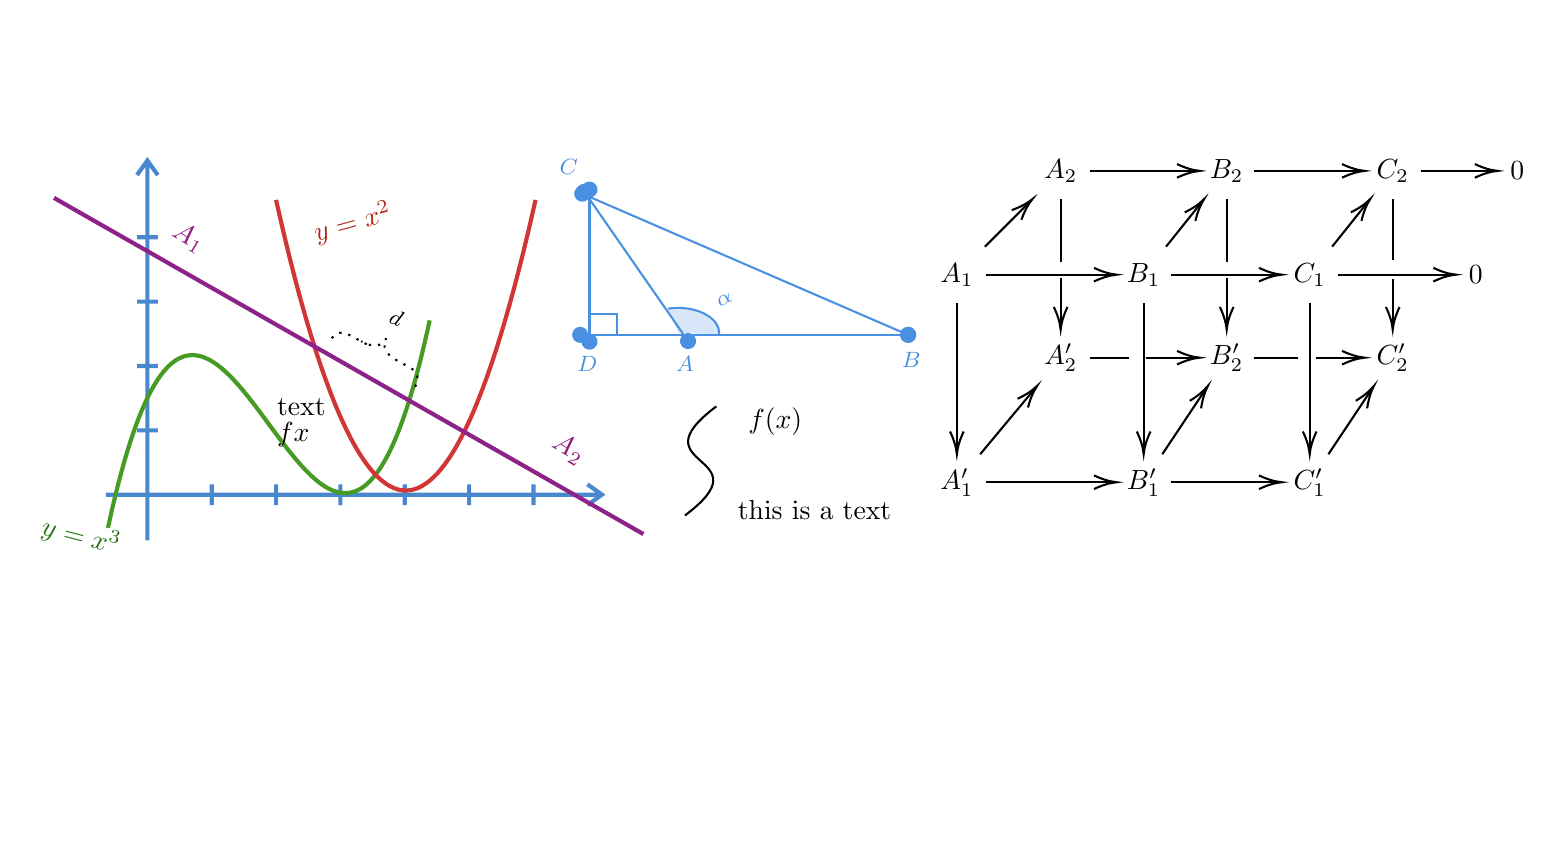
\begin{tikzpicture}[x=0.75pt,y=0.75pt,yscale=-1,xscale=1]
%uncomment if require: \path (0,235); %set diagram left start at 0, and has height of 235

%Straight Lines [id:da9313950171592851] 
\draw [color={rgb, 255:red, 74; green, 144; blue, 226 }  ,draw opacity=1 ]   (274,30) -- (274,103.29) ;
\draw [shift={(274,103.29)}, rotate = 90] [color={rgb, 255:red, 74; green, 144; blue, 226 }  ,draw opacity=1 ][fill={rgb, 255:red, 74; green, 144; blue, 226 }  ,fill opacity=1 ][line width=0.75]      (0, 0) circle [x radius= 3.35, y radius= 3.35]   ;
\draw [shift={(274,30)}, rotate = 90] [color={rgb, 255:red, 74; green, 144; blue, 226 }  ,draw opacity=1 ][fill={rgb, 255:red, 74; green, 144; blue, 226 }  ,fill opacity=1 ][line width=0.75]      (0, 0) circle [x radius= 3.35, y radius= 3.35]   ;
%Straight Lines [id:da0072983473385641595] 
\draw [color={rgb, 255:red, 74; green, 144; blue, 226 }  ,draw opacity=1 ]   (427.58,100) -- (269.5,100) ;
\draw [shift={(269.5,100)}, rotate = 180] [color={rgb, 255:red, 74; green, 144; blue, 226 }  ,draw opacity=1 ][fill={rgb, 255:red, 74; green, 144; blue, 226 }  ,fill opacity=1 ][line width=0.75]      (0, 0) circle [x radius= 3.35, y radius= 3.35]   ;
\draw [shift={(427.58,100)}, rotate = 180] [color={rgb, 255:red, 74; green, 144; blue, 226 }  ,draw opacity=1 ][fill={rgb, 255:red, 74; green, 144; blue, 226 }  ,fill opacity=1 ][line width=0.75]      (0, 0) circle [x radius= 3.35, y radius= 3.35]   ;
%Straight Lines [id:da0611422079179329] 
\draw [color={rgb, 255:red, 74; green, 144; blue, 226 }  ,draw opacity=1 ]   (270.5,32) -- (427.5,100) ;
\draw [shift={(427.5,100)}, rotate = 23.42] [color={rgb, 255:red, 74; green, 144; blue, 226 }  ,draw opacity=1 ][fill={rgb, 255:red, 74; green, 144; blue, 226 }  ,fill opacity=1 ][line width=0.75]      (0, 0) circle [x radius= 3.35, y radius= 3.35]   ;
\draw [shift={(270.5,32)}, rotate = 23.42] [color={rgb, 255:red, 74; green, 144; blue, 226 }  ,draw opacity=1 ][fill={rgb, 255:red, 74; green, 144; blue, 226 }  ,fill opacity=1 ][line width=0.75]      (0, 0) circle [x radius= 3.35, y radius= 3.35]   ;
%Straight Lines [id:da6902289836929021] 
\draw [color={rgb, 255:red, 74; green, 144; blue, 226 }  ,draw opacity=1 ]   (271.5,31) -- (321.5,103) ;
\draw [shift={(321.5,103)}, rotate = 55.22] [color={rgb, 255:red, 74; green, 144; blue, 226 }  ,draw opacity=1 ][fill={rgb, 255:red, 74; green, 144; blue, 226 }  ,fill opacity=1 ][line width=0.75]      (0, 0) circle [x radius= 3.35, y radius= 3.35]   ;
\draw [shift={(271.5,31)}, rotate = 55.22] [color={rgb, 255:red, 74; green, 144; blue, 226 }  ,draw opacity=1 ][fill={rgb, 255:red, 74; green, 144; blue, 226 }  ,fill opacity=1 ][line width=0.75]      (0, 0) circle [x radius= 3.35, y radius= 3.35]   ;
%Shape: Arc [id:dp012460516914444497] 
\draw  [draw opacity=0][fill={rgb, 255:red, 74; green, 144; blue, 226 }  ,fill opacity=0.22 ] (311.81,87.37) .. controls (313.42,87.12) and (315.12,86.99) .. (316.87,87) .. controls (327.75,87.07) and (336.54,92.5) .. (336.5,99.12) .. controls (336.5,99.34) and (336.49,99.56) .. (336.47,99.78) -- (316.8,99) -- cycle ; \draw  [color={rgb, 255:red, 74; green, 144; blue, 226 }  ,draw opacity=1 ] (311.81,87.37) .. controls (313.42,87.12) and (315.12,86.99) .. (316.87,87) .. controls (327.75,87.07) and (336.54,92.5) .. (336.5,99.12) .. controls (336.5,99.34) and (336.49,99.56) .. (336.47,99.78) ;
%Straight Lines [id:da012774030553635018] 
\draw [color={rgb, 255:red, 74; green, 144; blue, 226 }  ,draw opacity=1 ]   (274,90) -- (287.04,90) -- (287.04,100.78) ;
%Shape: Axis 2D [id:dp048941842347560494] 
\draw [color={rgb, 255:red, 73; green, 135; blue, 206 }  ,draw opacity=1 ][line width=1.5]  (41,177) -- (280,177)(61,16) -- (61,199) (273,172) -- (280,177) -- (273,182) (56,23) -- (61,16) -- (66,23) (92,172) -- (92,182)(123,172) -- (123,182)(154,172) -- (154,182)(185,172) -- (185,182)(216,172) -- (216,182)(247,172) -- (247,182)(56,146) -- (66,146)(56,115) -- (66,115)(56,84) -- (66,84)(56,53) -- (66,53) ;
\draw   ;
%Shape: Polynomial [id:dp29246577559714826] 
\draw  [color={rgb, 255:red, 70; green, 155; blue, 36 }  ,draw opacity=1 ][line width=1.5]  (42,193) .. controls (93.67,-47) and (145.33,333) .. (197,93) ;
%Shape: Parabola [id:dp636758281566334] 
\draw  [color={rgb, 255:red, 209; green, 53; blue, 53 }  ,draw opacity=1 ][line width=1.5]  (123,35) .. controls (164.67,221.67) and (206.33,221.67) .. (248,35) ;
%Straight Lines [id:da5751643928734858] 
\draw [color={rgb, 255:red, 141; green, 34; blue, 137 }  ,draw opacity=1 ][line width=1.5]    (16,34) -- (300,196) ;
%Shape: Brace [id:dp8862990797251067] 
\draw  [dash pattern={on 0.84pt off 2.51pt}] (190,125) .. controls (192.21,120.89) and (191.25,117.73) .. (187.14,115.52) -- (181.62,112.56) .. controls (175.75,109.41) and (173.91,105.77) .. (176.12,101.66) .. controls (173.91,105.77) and (169.87,106.25) .. (164,103.1)(166.64,104.52) -- (158.48,100.14) .. controls (154.37,97.93) and (151.21,98.89) .. (149,103) ;
%Curve Lines [id:da4259284507066625] 
\draw    (320,187) .. controls (360,157) and (295.13,164.46) .. (335.13,134.46) ;

% Text Node
\draw (339,83) node  [font=\footnotesize,color={rgb, 255:red, 74; green, 144; blue, 226 }  ,opacity=1 ,rotate=-333.43]  {$\alpha $};
% Text Node
\draw (264,19) node  [font=\footnotesize,color={rgb, 255:red, 74; green, 144; blue, 226 }  ,opacity=1 ]  {$C$};
% Text Node
\draw (273,114) node  [font=\footnotesize,color={rgb, 255:red, 74; green, 144; blue, 226 }  ,opacity=1 ]  {$D$};
% Text Node
\draw (320,114) node  [font=\footnotesize,color={rgb, 255:red, 74; green, 144; blue, 226 }  ,opacity=1 ]  {$A$};
% Text Node
\draw (429,112) node  [font=\footnotesize,color={rgb, 255:red, 74; green, 144; blue, 226 }  ,opacity=1 ]  {$B$};
% Text Node
\draw (451,71) node    {$A_{1}$};
% Text Node
\draw (501,21) node    {$A_{2}$};
% Text Node
\draw (451,171) node    {$A'_{1}$};
% Text Node
\draw (581,21) node    {$B_{2}$};
% Text Node
\draw (661,21) node    {$C_{2}$};
% Text Node
\draw (541,71) node    {$B_{1}$};
% Text Node
\draw (621,71) node    {$C_{1}$};
% Text Node
\draw (501,111) node    {$A'_{2}$};
% Text Node
\draw (581,111) node    {$B'_{2}$};
% Text Node
\draw (661,111) node    {$C'_{2}$};
% Text Node
\draw (541,171) node    {$B'_{1}$};
% Text Node
\draw (621,171) node    {$C'_{1}$};
% Text Node
\draw (721,21) node    {$0$};
% Text Node
\draw (701,71) node    {$0$};
% Text Node
\draw (81,53) node  [color={rgb, 255:red, 146; green, 29; blue, 130 }  ,opacity=1 ,rotate=-30.96]  {$A_{1}$};
% Text Node
\draw (264,155) node  [color={rgb, 255:red, 145; green, 25; blue, 123 }  ,opacity=1 ,rotate=-30.96]  {$A_{2}$};
% Text Node
\draw (29,197) node  [color={rgb, 255:red, 36; green, 114; blue, 18 }  ,opacity=1 ,rotate=-14.47]  {$y=x^{3}$};
% Text Node
\draw (160,46) node  [color={rgb, 255:red, 179; green, 35; blue, 24 }  ,opacity=1 ,rotate=-344.74]  {$y=x^{2}$};
% Text Node
\draw (181,92) node  [font=\footnotesize,rotate=-22.93]  {$d$};
% Text Node
\draw (122,129) node [anchor=north west][inner sep=0.75pt]   [align=left] {text};
% Text Node
\draw (122,140.4) node [anchor=north west][inner sep=0.75pt]    {$fx$};
% Text Node
\draw (344,178) node [anchor=north west][inner sep=0.75pt]   [align=left] {this is a text};
% Text Node
\draw (349,133.4) node [anchor=north west][inner sep=0.75pt]    {$f( x)$};
% Connection
\draw    (515,21) -- (566,21) ;
\draw [shift={(568,21)}, rotate = 180] [color={rgb, 255:red, 0; green, 0; blue, 0 }  ][line width=0.75]    (10.93,-3.29) .. controls (6.95,-1.4) and (3.31,-0.3) .. (0,0) .. controls (3.31,0.3) and (6.95,1.4) .. (10.93,3.29)   ;
% Connection
\draw    (594,21) -- (645.5,21) ;
\draw [shift={(647.5,21)}, rotate = 180] [color={rgb, 255:red, 0; green, 0; blue, 0 }  ][line width=0.75]    (10.93,-3.29) .. controls (6.95,-1.4) and (3.31,-0.3) .. (0,0) .. controls (3.31,0.3) and (6.95,1.4) .. (10.93,3.29)   ;
% Connection
\draw    (464.5,57.5) -- (486.09,35.91) ;
\draw [shift={(487.5,34.5)}, rotate = 495] [color={rgb, 255:red, 0; green, 0; blue, 0 }  ][line width=0.75]    (10.93,-3.29) .. controls (6.95,-1.4) and (3.31,-0.3) .. (0,0) .. controls (3.31,0.3) and (6.95,1.4) .. (10.93,3.29)   ;
% Connection
\draw    (465,71) -- (526,71) ;
\draw [shift={(528,71)}, rotate = 180] [color={rgb, 255:red, 0; green, 0; blue, 0 }  ][line width=0.75]    (10.93,-3.29) .. controls (6.95,-1.4) and (3.31,-0.3) .. (0,0) .. controls (3.31,0.3) and (6.95,1.4) .. (10.93,3.29)   ;
% Connection
\draw    (554,71) -- (605.5,71) ;
\draw [shift={(607.5,71)}, rotate = 180] [color={rgb, 255:red, 0; green, 0; blue, 0 }  ][line width=0.75]    (10.93,-3.29) .. controls (6.95,-1.4) and (3.31,-0.3) .. (0,0) .. controls (3.31,0.3) and (6.95,1.4) .. (10.93,3.29)   ;
% Connection
\draw    (551.8,57.5) -- (568.95,36.06) ;
\draw [shift={(570.2,34.5)}, rotate = 488.66] [color={rgb, 255:red, 0; green, 0; blue, 0 }  ][line width=0.75]    (10.93,-3.29) .. controls (6.95,-1.4) and (3.31,-0.3) .. (0,0) .. controls (3.31,0.3) and (6.95,1.4) .. (10.93,3.29)   ;
% Connection
\draw    (631.8,57.5) -- (648.95,36.06) ;
\draw [shift={(650.2,34.5)}, rotate = 488.66] [color={rgb, 255:red, 0; green, 0; blue, 0 }  ][line width=0.75]    (10.93,-3.29) .. controls (6.95,-1.4) and (3.31,-0.3) .. (0,0) .. controls (3.31,0.3) and (6.95,1.4) .. (10.93,3.29)   ;
% Connection
\draw    (451,84.5) -- (451,155.5) ;
\draw [shift={(451,157.5)}, rotate = 270] [color={rgb, 255:red, 0; green, 0; blue, 0 }  ][line width=0.75]    (10.93,-3.29) .. controls (6.95,-1.4) and (3.31,-0.3) .. (0,0) .. controls (3.31,0.3) and (6.95,1.4) .. (10.93,3.29)   ;
% Connection
\draw    (465,171) -- (526,171) ;
\draw [shift={(528,171)}, rotate = 180] [color={rgb, 255:red, 0; green, 0; blue, 0 }  ][line width=0.75]    (10.93,-3.29) .. controls (6.95,-1.4) and (3.31,-0.3) .. (0,0) .. controls (3.31,0.3) and (6.95,1.4) .. (10.93,3.29)   ;
% Connection
\draw    (554,171) -- (605.5,171) ;
\draw [shift={(607.5,171)}, rotate = 180] [color={rgb, 255:red, 0; green, 0; blue, 0 }  ][line width=0.75]    (10.93,-3.29) .. controls (6.95,-1.4) and (3.31,-0.3) .. (0,0) .. controls (3.31,0.3) and (6.95,1.4) .. (10.93,3.29)   ;
% Connection
\draw    (630,157.5) -- (650.89,126.16) ;
\draw [shift={(652,124.5)}, rotate = 483.69] [color={rgb, 255:red, 0; green, 0; blue, 0 }  ][line width=0.75]    (10.93,-3.29) .. controls (6.95,-1.4) and (3.31,-0.3) .. (0,0) .. controls (3.31,0.3) and (6.95,1.4) .. (10.93,3.29)   ;
% Connection
\draw    (550,157.5) -- (570.89,126.16) ;
\draw [shift={(572,124.5)}, rotate = 483.69] [color={rgb, 255:red, 0; green, 0; blue, 0 }  ][line width=0.75]    (10.93,-3.29) .. controls (6.95,-1.4) and (3.31,-0.3) .. (0,0) .. controls (3.31,0.3) and (6.95,1.4) .. (10.93,3.29)   ;
% Connection
\draw    (462.25,157.5) -- (488.47,126.04) ;
\draw [shift={(489.75,124.5)}, rotate = 489.81] [color={rgb, 255:red, 0; green, 0; blue, 0 }  ][line width=0.75]    (10.93,-3.29) .. controls (6.95,-1.4) and (3.31,-0.3) .. (0,0) .. controls (3.31,0.3) and (6.95,1.4) .. (10.93,3.29)   ;
% Connection
\draw    (515,111) -- (533.95,111)(541.95,111) -- (566,111) ;
\draw [shift={(568,111)}, rotate = 180] [color={rgb, 255:red, 0; green, 0; blue, 0 }  ][line width=0.75]    (10.93,-3.29) .. controls (6.95,-1.4) and (3.31,-0.3) .. (0,0) .. controls (3.31,0.3) and (6.95,1.4) .. (10.93,3.29)   ;
% Connection
\draw    (594,111) -- (615.25,111)(624.25,111) -- (645.5,111) ;
\draw [shift={(647.5,111)}, rotate = 180] [color={rgb, 255:red, 0; green, 0; blue, 0 }  ][line width=0.75]    (10.93,-3.29) .. controls (6.95,-1.4) and (3.31,-0.3) .. (0,0) .. controls (3.31,0.3) and (6.95,1.4) .. (10.93,3.29)   ;
% Connection
\draw    (501,34.5) -- (501,64.66)(501,72.66) -- (501,95.5) ;
\draw [shift={(501,97.5)}, rotate = 270] [color={rgb, 255:red, 0; green, 0; blue, 0 }  ][line width=0.75]    (10.93,-3.29) .. controls (6.95,-1.4) and (3.31,-0.3) .. (0,0) .. controls (3.31,0.3) and (6.95,1.4) .. (10.93,3.29)   ;
% Connection
\draw    (581,34.5) -- (581,64.66)(581,72.66) -- (581,95.5) ;
\draw [shift={(581,97.5)}, rotate = 270] [color={rgb, 255:red, 0; green, 0; blue, 0 }  ][line width=0.75]    (10.93,-3.29) .. controls (6.95,-1.4) and (3.31,-0.3) .. (0,0) .. controls (3.31,0.3) and (6.95,1.4) .. (10.93,3.29)   ;
% Connection
\draw    (661,34.5) -- (661,64.16)(661,73.16) -- (661,95.5) ;
\draw [shift={(661,97.5)}, rotate = 270] [color={rgb, 255:red, 0; green, 0; blue, 0 }  ][line width=0.75]    (10.93,-3.29) .. controls (6.95,-1.4) and (3.31,-0.3) .. (0,0) .. controls (3.31,0.3) and (6.95,1.4) .. (10.93,3.29)   ;
% Connection
\draw    (541,84.5) -- (541,155.5) ;
\draw [shift={(541,157.5)}, rotate = 270] [color={rgb, 255:red, 0; green, 0; blue, 0 }  ][line width=0.75]    (10.93,-3.29) .. controls (6.95,-1.4) and (3.31,-0.3) .. (0,0) .. controls (3.31,0.3) and (6.95,1.4) .. (10.93,3.29)   ;
% Connection
\draw    (621,84.5) -- (621,155.5) ;
\draw [shift={(621,157.5)}, rotate = 270] [color={rgb, 255:red, 0; green, 0; blue, 0 }  ][line width=0.75]    (10.93,-3.29) .. controls (6.95,-1.4) and (3.31,-0.3) .. (0,0) .. controls (3.31,0.3) and (6.95,1.4) .. (10.93,3.29)   ;
% Connection
\draw    (674.5,21) -- (709.5,21) ;
\draw [shift={(711.5,21)}, rotate = 180] [color={rgb, 255:red, 0; green, 0; blue, 0 }  ][line width=0.75]    (10.93,-3.29) .. controls (6.95,-1.4) and (3.31,-0.3) .. (0,0) .. controls (3.31,0.3) and (6.95,1.4) .. (10.93,3.29)   ;
% Connection
\draw    (634.5,71) -- (689.5,71) ;
\draw [shift={(691.5,71)}, rotate = 180] [color={rgb, 255:red, 0; green, 0; blue, 0 }  ][line width=0.75]    (10.93,-3.29) .. controls (6.95,-1.4) and (3.31,-0.3) .. (0,0) .. controls (3.31,0.3) and (6.95,1.4) .. (10.93,3.29)   ;

\end{tikzpicture}



\section{随机变量的引入}

在实际问题中,随机试验的结果可以用数量来表示,由此就产生了随机变量的概念.

有些试验结果本身与数值有关(本身就是一个数);在有些试验中,试验结果看来与数值无关,但我们可以引进一个变量来表示它的各种结果.也就是说,把试验结果数值化.这种对应关系在数学上理解为定义了一种实值单值函数

\section{随机变量的特点}

它随试验结果的不同而取不同的值,因而在试验之前只知道它可能取值的范围,而不能预先肯定它将取哪个值.

由于试验结果的出现具有一定的概率,于是这种实值函数取每个值和每个确定范围内的值也有一定的概率, 所以称这种定义在样本空间 $S$ 上的实值单值函数 $X= X(e)$为随机变量

\section{优势}

\begin{enumerate}
    \item 引入随机变量后,对随机现象统计规律的研究,就由对事件及事件概率的研究扩大为对随机变量及其取值规律的研究
    \item 易于表示
    \item 和原来集合的表示等价
\end{enumerate}

\section{常见随机变量}

\subsection{离散型随机变量}

公式法

$$
\boldsymbol{P}\left\{\boldsymbol{X}=\boldsymbol{x}_{k}\right\}=\boldsymbol{p}_{k}, \boldsymbol{k}=1,2, \cdots
$$

列表法
  
$$X \sim\left(\begin{array}{lllll}x_{1} & x_{2} & \cdots & x_{n} & \cdots \\ p_{1} & p_{2} & \cdots & p_{n} & \cdots\end{array}\right)$$

\begin{center}
    \begin{tabular}{|c|c|c|c|c|}
    \hline $ \boldsymbol{X} $ & $ \boldsymbol{x}_{1} $ & $ \boldsymbol{x}_{2} $ & $ \cdots $ & $ \boldsymbol{x}_{n} \cdots $ \\
    \hline $ \boldsymbol{p}_{k} $ & $ \boldsymbol{p}_{1} $ & $ \boldsymbol{p}_{2} $ & $ \cdots $ & $ \boldsymbol{p}_{n} \cdots $ \\
    \hline
    \end{tabular}
\end{center}


\subsection{两点分布}

特殊的二项分布(n = 1)
\begin{center}
   \begin{tabular}{|c|c|c|}
    \hline $ \mathrm{X} $ & $0$ & $1 $\\
    \hline$ p_{k} $ & $ 1-\mathrm{p} $ & $ \mathrm{p} $ \\
    \hline
    \end{tabular}

\subsection{(n 重)伯努利试验, 二项分布} 
\end{center}


$$
P\{X=k\}=\left(\begin{array}{l}
n \\
k
\end{array}\right) p^{k}(1-p)^{n-k} \quad k=0,1, \cdots, n
$$

$$
\begin{array}{c|cccccc}
\boldsymbol{X} & \mathbf{0} & \mathbf{1} & \cdots & \boldsymbol{k} & \cdots & \boldsymbol{n} \\
\hline \boldsymbol{p}_{\boldsymbol{k}} & \boldsymbol{q}^{n} & \left(\begin{array}{l}
\boldsymbol{n} \\
\mathbf{1}
\end{array}\right) \boldsymbol{p q}^{n-1} & \cdots & \left(\begin{array}{l}
\boldsymbol{n} \\
\boldsymbol{k}
\end{array}\right) \boldsymbol{p}^{k} \boldsymbol{q}^{n-k} & \cdots & \boldsymbol{p}^{n}
\end{array}
$$

\subsubsection{二项分布性质}

\begin{itemize}
    \item 将伯努利试验 $E$独立地重复地进行 $n$ 次 ,则称这一串重复的独立试验为 $n$ 重伯努利试验.伯努利试验对试验结果没有等可能的要求 “重复”是指这 $n$ 次试验中 $P(A)= p$ 保持不变.“独立”是指各次试验的结果互不影响.
    \item 每次试验条件相同
    \item 每次试验只考虑两个互逆结果 $A$ 或 $\overline{A}$
    \item 各次试验相互独立
    \item 二项分布描述的是 $n$ 重伯努利试验中事件 $A$ 出现的次数 $X$ 的分布律
\end{itemize}

\subsubsection{二项分布单峰性质}

若在$k_0$处,概率 P{X=k}达到最大(称$k_0$为随机变量 X 的最可能值)

$$
\left\{\begin{array}{l}
\frac{P\left\{X=k_{0}\right\}}{P\left\{X=k_{0}+1\right\}} \geq 1 \\
\frac{P\left\{X=k_{0}\right\}}{P\left\{X=k_{0}-1\right\}} \geq 1
\end{array}\right.
$$

得
$$ (n+1) p-1 \leq k\_{0} \leq(n+1) p $$

$$
k_{0}=\left\{\begin{array}{ll}
(n+1) p \text { 和 }(n+1) p-1, & \text { 当 }(\boldsymbol{n}+\mathbf{1}) \boldsymbol{p} \text { 为整数 }, \\
{[(n+1) p],} & \text { 其它 },
\end{array}\right.
$$

\subsection{泊松分布}

$$
\boldsymbol{P}\{\boldsymbol{X}=\boldsymbol{k}\}=\frac{\lambda^{k} \mathrm{e}^{-\lambda}}{\boldsymbol{k} !}, \quad \boldsymbol{k}=\mathbf{0}, \mathbf{1}, \mathbf{2}, \cdots
$$

其中$\lambda > 0$是常数, 则称 X 服从参数为$\lambda$的泊松分布, 记作
$$ X \sim \pi(\lambda) $$


\begin{theorem}[泊松定理]
    \label{thm:Poission}
泊松分布是作为二项分布的近似,于 1837 年由法国数学家泊松引入的.
$$
\lim _{n \rightarrow \infty} C_{n}^{k} p_{n}^{k}\left(1-p_{n}\right)^{n-k}=e^{-\lambda} \frac{\lambda^{k}}{k !}\quad (\lambda = np)
$$
\end{theorem}

\subsection{连续型随机变量}

\subsection{均匀分布}

$$
f(x)=\left\{\begin{array}{cc}
\frac{1}{b-a}, & a<x<b \\
0, & \text { 其它 }
\end{array}\right.
$$

$$ X \sim U(a,b) $$

$$
F(x)=P\{X \leq x\}=\left\{\begin{array}{ll}
0, & x<a \\
\frac{x-a}{b-a}, & a \leq x<b \\
1 & x \geq b
\end{array}\right.
$$

\subsection{指数分布}

$$
f(x)=\left\{\begin{array}{ll}
\frac{1}{\theta} e^{-x / \theta}, & x>0 \\
0, & \text { 其它, }
\end{array}\right.
$$

$$
F(x)=P\{X \leq x\}=\left\{\begin{array}{ll}
1-e^{-x / \theta}, & x>0 \\
0, & \text { 其它 }
\end{array}\right.
$$

\subsection{正态分布}

$$
f(x)=\frac{1}{\sqrt{2 \pi} \sigma} e^{-\frac{(x-\mu)^{2}}{2 \sigma^{2}}}, \quad-\infty<x<\infty
$$

\subsection{标准正态分布}

$$
\text { 若 } X \sim N\left(\mu, \sigma^{2}\right), \text { 则 } Z=\frac{X-\mu}{\sigma} \sim N(\mathbf{0}, 1)
$$

\section{随机变量的分布函数}

\section{随机变量的分布函数性质}

对任意实数 $x_1<x_2$,随机点落在区间$( x_1 ,  x_2 ]$内的概率为:

$$
P\{ x_1<X  \le  x_2\} =P\{ X  \le   x_2 \} - P\{ X  \le   x_1 \}= F(x_2)-F(x_1)
$$

$$
\begin{array}{l}
F(-\infty)=\lim_{x \rightarrow-\infty} F(x)=0 \\
F(+\infty)=\lim_{x \rightarrow+\infty} F(x)=1
\end{array}
$$

\section{连续型随机变量及其概率密度}

$$ f(x) \geq 0 $$

$$ \int\_{-\infty}^{\infty} f(x) d x=1 $$

% todo: 边缘分布、条件分布

\section{随机变量的数字特征}

\subsection{方差}


$$
 D(X) = E \Big\{ [x-E(X)] \Big\}
$$

$$
 D(X) = E(X^2) - [E(X)] ^2
$$

\subsubsection{方差性质}

$$
 D(C) = 0
$$

$$
 D(CX) = C^2D(X)
$$

$$
 D(X+C) = D(X)
$$

X 和 Y 相互独立时,

$$
 D(X+Y) = D(X)+D(Y)
$$

D(X) = 0 等价于 $
 P[X = E(X)] = 1
$

\begin{theorem}[切比雪夫不等式]
    \label{Chebyshev\'sInequality}
$$
\begin{aligned}
    P(|X-\mu| \ge \varepsilon) \le \frac{\sigma^2}{\varepsilon^2}
\end{aligned}
$$

$$
 P(|X-\mu| < \varepsilon) \ge 1 - \frac{\sigma^2}{\varepsilon^2}
$$
\end{theorem}

\subsection{协方差}

$$
 Cov(X,Y) = E\Big\{ [X - E(X)][Y-E(Y)] \Big\}
$$

$$
 Cov(X,Y) = E(XY) - E(X)E(Y)
$$

\subsubsection{协方差性质}

$$
 D(X+Y) = D(X)+D(Y)+2Cov(X,Y)
$$

$$
 Cov(X,Y) = Cov(Y,X)
$$

$$
 Cov(X,X) = D(X)
$$

$$ Cov(X,c) = 0 $$

$$ Cov(a X + b, Y) = a Cov( X,Y) $$

$$ Cov(aX, bY) = ab Cov(X, Y) $$

$$ Cov(X_1 + X_2 , Y) = Cov(X_1 , Y) + Cov(X_2 , Y) $$

对于随机变量序列 $ X_{1}, \ldots, X_{n} $ 与 $ Y_{1}, \ldots, Y_{m} $, 有
$$
\operatorname{cov}\left(\sum_{i=1}^{n} X_{i}, \sum_{j=1}^{m} Y_{j}\right)=\sum_{i=1}^{n} \sum_{j=1}^{m} \operatorname{cov}\left(X_{i}, Y_{j}\right)
$$

对于随机变量序列 $ X_{1}, \ldots, X_{n} $, 有

$$
\operatorname{var}\left(\sum_{i=1}^{n} X_{i}\right)=\sum_{i=1}^{n} \operatorname{var}\left(X_{i}\right)+2 \sum_{i, j: i<j} \operatorname{cov}\left(X_{i}, X_{j}\right)
$$

\subsection{相关系数}

$$
 \rho_{XY} =   \frac{Cov(X,Y) }{\sqrt{D(X)} \sqrt{D(Y)}}
$$

相关系数是刻划两个变量间线性相关程度的一个重要的数字特征. 相关系数也可以看成协方差:一种剔除了两个变量量纲影响、标准化后的特殊协方差。

\subsection{X, Y 不相关时候的性质}

若 $\rho_{X Y}=0$, 称 X 和 Y 不(线性)相关。

\begin{corollary}
    独立一定是不相关,不相关不一定独立。
\end{corollary}

\begin{theorem}
    若随机变量 $X$ 与 Y 的方差都存在,且均不为零; 则下列四个命题等价。
    \begin{enumerate}
        \item $\rho_{X Y}=0$
        \item $\operatorname{Cov}(X, Y)=0$
        \item $E(X Y)=E (X) E (Y)$
        \item $D(X \pm Y)=D X+D Y_{\circ}$
    \end{enumerate}
\end{theorem}

% \chapter{大数定律和中心极限定理}
% \section{辛钦大数定律}

\begin{theorem}[辛钦大数定律]
    设随机变量序列$X_1,X_2, …$   相互独立, 服从同一分布, 具有数学期$E(X_i)=\mu, i=1,2,…$,  则对于任意正数ε , 有

$$\lim _{n \rightarrow \infty} P\left\{\left|\frac{1}{n} \sum_{i=1}^{n} X_{i}-\mu\right|<\varepsilon\right\}=1$$

则序列$\bar{X}=\frac{1}{n} \sum_{i=1}^{n} X_{i}$ 依概率收敛于$\mu$(很可能接近于$\mu$)。
\end{theorem}

另一表述:
$$\overline{X} \rightarrow^{P} \mu$$

\subsection{辛钦大数定律条件}

\begin{itemize}
    \item $X_1,X_2, …$ 相互独立
    \item $X_1,X_2, …$ 服从同一分布
    \item 不要求方差存在。 
\end{itemize}

\begin{corollary}
设${X_n \rightarrow^{P} a}$, ${Y_n \rightarrow^{P} b}$则

$$
   g(X_n, Y_n) \rightarrow^{P} g(a,b)
$$
\end{corollary}

\section{伯努利大数定理}

\begin{theorem}[伯努利大数定理]
设$f_A$是n次独立重复试验中事件A的发生次数, p是每次试验中发生的概率, 则对于任意的正数$\varepsilon$.

$$
 \lim_{n \to \infty}\{ |f_A/n - p| < \varepsilon\} = 1  
$$
\end{theorem}

贝努里大数定律表明, 当重复试验次数n充分大时, 事件A发生的频率nA/n与事件A的概率p有较大偏差的概率很小。

\section{中心极限定理}

\begin{theorem}[Lyapunov中心极限定理]
    设$X_1,X_2,...$相互独立,他们拥有数学期望和方差

$$
 E(X_k) = \mu_k
$$

$$
  D(X_k) = \sigma_k^2
$$
则有

$$
\begin{aligned} \lim _{n \rightarrow \infty} F_{n}(x) &=\lim _{n \rightarrow \infty} P\left\{\frac{\sum_{k=1}^{n} X_{k}-\sum_{k=1}^{n} \mu_{k}}{B_{n}} \leq x\right\}
\\ &=\int_{-\infty}^{x} \frac{1}{\sqrt{2 \pi}} \mathrm{e}^{-\mathrm{t}^{2} / 2} \mathrm{~d} \mathrm{t}
\\&=\Phi(x)
 \end{aligned}
 $$

其中$B_n=\sqrt{D\left(\sum_{k=1}^{n} X_{k}\right)}$
\end{theorem}

\begin{theorem}
    设$X_1,X_2,...$相互独立,他们服从同一分布,拥有数学期望和方差

$$
 E(X_k) = \mu
$$

$$
  D(X_k) = \sigma^2
$$
则有

$$\begin{aligned}
\lim _{n \rightarrow \infty} F_{n}(x)&=\lim _{n \rightarrow \infty} P\left\{\frac{\sum_{i=1}^{n} X_{i}-n \mu}{\sigma \sqrt{n}} \leq x\right\}
\\ &=\int_{-\infty}^{x} \frac{1}{\sqrt{2 \pi}} \mathrm{e}^{-\mathrm{t}^{2} / 2} \mathrm{~d} \mathrm{t}
\\&=\Phi(x)
\end{aligned}
$$
\end{theorem}

\begin{theorem}[De Moivre-Laplace定理]
设$\eta_{n}$服从参数为n,p的二项分布, 则对于任意$x$,有
$$
\lim _{n \rightarrow \infty} P\left\{\frac{\eta_{n}-n p}{\sqrt{n p(1-p)}} \leq x\right\}=\int_{-\infty}^{x} \frac{1}{\sqrt{2 \pi}} e^{-\frac{t^{2}}{2}} d t=\Phi(x)
$$
\end{theorem}

\begin{proof}
    将$\eta_{n}$拆分成$n$个相互独立,服从同一分布的随机变量$X_1,X_2,...$之和
\end{proof}




% % todo: 样本与总体
% \chapter{Sampling Distribution}
% \section{统计量}

不含任何未知参数的样本的函数称为统计量.
它是完全由样本决定的量.

\section{常见统计量}

\begin{definition}[样本平均值]
    $$\overline{X}=\frac{1}{n} \sum_{i=1}^{n} X_{i}$$
\end{definition}

\begin{definition}[样本方差]
    $$S^{2}=\frac{1}{ n-1} \sum_{i=1}^{n}\left(X_{i}-\bar{X}\right)^{2}$$
\end{definition}

\begin{definition}[样本标准差]
    $$S=\sqrt{\frac{1}{ { n-1} } \sum_{i=1}^{n}\left(X_{i}-\bar{X}\right)^{2}}$$
\end{definition}

\begin{definition}[样本 $k$ 阶原点矩]
    $$A_{k}=\frac{1}{n} \sum_{i=1}^{n} X_{i}^{k}$$
\end{definition}

\begin{definition}[样本 $k$ 阶中心矩]
    $$\boldsymbol{B}_{\boldsymbol{k}}=\frac{1}{\boldsymbol{n}} \sum_{i=1}^{n}\left(\boldsymbol{X}_{i}-\overline{\boldsymbol{X}}\right)^{k}$$
\end{definition}

\begin{definition}[$X$和$Y$的$k+p$阶混合原点矩]
    若
    $$E \left\{\left(X^ k\right)\left(Y^ p\right)\right\}, k, p=1,2, \ldots $$
    存在, 则称它为$X$和$Y$的$k+p$阶混合原点矩
\end{definition}

\begin{definition}[$X$和$Y$的$k+l$阶混合中心矩]
    若
    $$ E\left\{[X-E(X)]^ k[Y-E(Y)]^l \right\},  k,l=1, \quad 2, \ldots $$
    存在, 则称它为$X$和$Y$的$k+l$阶混合中心矩
\end{definition}



\section{卡方分布}

\begin{definition}[卡方分布]
    设$X_1,X_2,...X_n$相互独立, 都服从正态分布 $N(0,1)$ (都是来自总体 $N(0,1)$ 的样本), 则称随机变量:

    $$
        \chi^2 = X_1^2 + X_2^2 + ... + X_n^2
    $$

    所服从的分布为自由度为 $n$ 的$\chi^2$分布. 记作$\chi^2 \sim \chi^2(n)$
\end{definition}

\subsection{卡方分布性质}

\begin{corollary}
    $\chi^2(1) \sim X^2(1)$
\end{corollary}

\begin{corollary}[$\chi^2$分布的可加性]
    若 $ X_{1} \sim \chi^{2}\left(n_{1}\right), X_{2} \sim \chi^{2}\left(n_{2}\right) $, 且 $ X_{1} $ 与 $ X_{2} $ 相互独立,则
    $$
        X_{1}+X_{2} \sim \chi^{2}\left(n_{1}+n_{2}\right)
    $$
\end{corollary}

\begin{proof}
    事实上, 卡方分布是Gamma分布的特殊情况. 自由度为 $ n $ 的卡方分布 $ \chi_{n}^{2} $ 其实就是 $ \Gamma\left(\frac{n}{2}, \frac{1}{2}\right) $.

    根据Gamma分布的矩生成函数(Moment Generating Function, MGF),若$ X_{1} \sim \chi_{n_{1}}^{2} $,$ X_{2} \sim \chi_{n_{2}}^{2} $,

    那么 $ X_{1}, X_{2} $ 对应的MGF分别为
    $$ M_{X_{1}}(t)=(1-2 t)^{-n_{1} / 2} $$
    $$ M_{X_{2}}(t)=(1-2 t)^{-n_{2} / 2} $$
    因为 $ X_{1}, X_{2} $ 相互独立, 那么 $ Y=X_{1}+X_{2} $ 的MGF为
    $$ M_{Y}(t)=M_{X_{1}}(t) M_{X_{2}}(t)=(1-2 t)^{-\left(n_{1}+n_{2}\right) / 2} $$

    由MGF的唯一性,
    $$ \quad Y \sim \Gamma\left(\frac{n_{1}+n_{2}}{2}, \frac{1}{2}\right)=\chi_{n_{1}+n_{2}}^{2} $$
\end{proof}

\begin{corollary}[$\chi^2$分布的数学期望和方差]
    $$E(\chi^2) = n$$
    $$D(\chi^2) = 2n$$
\end{corollary}

\begin{proof}
    $$
        E(X) = 0\\
        D(X) = 1\\
        E(X_i^2) = 1\\
        D(X_i^2) = 2
    $$
\end{proof}

\begin{corollary}[卡方分布中心极限定理]
    设$X_1,X_2,...X_n$相互独立, 都服从正态分布 N(0,1), $E(X)=\mu$, $D(X)=\sigma^2$, 则有
    $$
        P(\frac{\chi^2(n)-n}{\sqrt{2n}} \le x) \sim \Phi(x)
    $$
\end{corollary}

\begin{proof}
    $$
        E(X) = 0\\
        D(X) = 1\\
        E(X_i^2) = 1\\
        D(X_i^2) = 2
    $$
\end{proof}

\begin{corollary}
    $$
        \frac{\chi^2(n)}{n} \leftarrow  \frac{1}{n} \sum^n_{i=1} X_i^2 = 1
    $$
\end{corollary}

\begin{proof}
    $$
        E(X_i^2) = 1
    $$
\end{proof}

\begin{definition}[卡方分布的上分位点]
    $$
        p(\chi^2 > \chi^2_\alpha(n)) = \alpha
    $$
\end{definition}

\section{t 分布}

\begin{definition}[自由度为 $t$ 的 t 分布]
    设$X \sim N(0,1), Y \sim \chi^2(n)$,且 X,Y 相互独立,则称随机变量

    $$
        t = \frac{X}{\sqrt{Y/n}}
    $$

    为自由度为 $n$ 的 t 分布, 记作$t \sim t(n)$

\end{definition}

\subsection{t 分布性质}

\begin{corollary}[t 分布数学期望和方差]
    $$
        E(t) = 0
    $$
    $$
        D\big(t(n)\big) = \frac{n}{n-2}
    $$
\end{corollary}

\begin{corollary}[t 分布的概率密度函数]
    $n = 1$时 $$f(t)=\frac{1}{\pi (1+t^2)}(柯西密度)$$ 数学期望不存在.
    $n>1$时, $h(t)$的图形关于 $t=0$ 对称.
\end{corollary}

\begin{corollary}
    $n$ 足够大时 t 分布近似于 $N(0,1)$ 分布. 由于卡方分布
    $$
        n\to \infty 时, \frac{\chi^2(n)}{n} \to 1
    $$
    所以
    $$
        \begin{aligned}
            t(n) =
            \ce{\frac{N(0,1)}{\sqrt{\frac{\chi^2(n)}{n}}}
            ->[n \to \infty]
            N(0,1)}
        \end{aligned}
    $$
\end{corollary}

\begin{corollary}[与 F 分布的关系]
    $$
        \begin{aligned}
            t^2(n) & = \frac{N(0,1)^2}{\chi^2 (n)/n}                    \\
                   & = \frac{\chi ^2(1)/1}{ \chi ^2(n) / n} \sim F(1,n)
        \end{aligned}
    $$

    $$
        \frac{1}{t^2(n)} \sim F(n,1)
    $$
\end{corollary}

\begin{definition}[t 分布的上分位点]
    $$
        t_{1-\alpha} (n) = -t_\alpha(n)
    $$
\end{definition}

\section{F 分布}

\begin{definition}[F 分布]
    设$U \sim \chi^2(n_1), V \sim \chi^2(n_2)$, 且 U, V 相互独立, 则称随机变量

    $$
        F = \frac{U/n_1}{V/n_2}
    $$

    服从自由度为$n_1,n_2$的 F 分布. 记作$F \sim F(n_1,n_2)$
\end{definition}

\subsection{F 分布性质}

\begin{corollary}[F 分布数学期望]
    $$
        E(F) =\frac{{ n_2} }{{ n_2}  - 2}
    $$

    即与$n_1$无关.
\end{corollary}

\begin{corollary}[$F(n_1,n_2),F(n_2,n_1)$的关系]
    $$
        \frac{1}{F(n_1,n_2)} \sim F(n_2,n_1)
    $$
\end{corollary}

\begin{corollary}[与 t 分布的关系]
    $$
        \begin{aligned}
            t^2(n) & = \frac{N(0,1)^2}{\chi^2 (n)/n}                    \\
                   & = \frac{\chi ^2(1)/1}{ \chi ^2(n) / n} \sim F(1,n)
        \end{aligned}
    $$

    $$
        \frac{1}{t^2(n)} \sim F(n,1)
    $$
\end{corollary}

\begin{corollary}[F 分布上 α 分位点的性质]
    $$
        F_{1-\alpha} (n_1,n_2) = \frac{1}{F_\alpha(n_2,n_1)}
    $$
\end{corollary}

\section{正态总体的样本均值和样本方差的分布}

\begin{definition}[正态总体的样本均值的数学期望、方差和样本方差的数学期望]
    设总体$X\sim N(\mu,\sigma^2)$的均值为$\mu$, 方差为$σ^2$.

    $X_1,X_2,...X_n$是来自$X$的一个样本, 样本均值是$\overline{X}$,样本方差是$S^2$,则有

    $$
        E(\overline{X}) = { \mu}
    $$

    $$
        D(\overline{ X}) =  {\frac{\sigma^2}{n}}
    $$

    $$
        E(S^2) = { \sigma^2}
    $$
\end{definition}

\begin{corollary}[矩估计法原理]
    $$\overline{X}=\frac{1}{n} \sum_{i=1}^{n} X_{i} \to E(X)$$

    $$\frac{1}{n} \sum X_1^2 - \overline{X}^2 \to D(X) = E(X^2) - E(X)^2$$
\end{corollary}

\begin{theorem}[样本均值的分布]
    设总体 X~N($\mu,\sigma^2$)的均值为$\mu$, 方差为$σ^2$, $X_1,X_2,...X_n$是来自$X$的一个样本, 样本均值是$\overline{X}$,则有

    $$
        {\overline{X} \sim N(\mu,\sigma^2/n) }
    $$
\end{theorem}

\begin{proof}
    $$
        \sum^n_{i=1} X_i = X_1 + X_2 + ...\sim N(n\mu, n\sigma^2)
    $$
\end{proof}

\begin{corollary}
    $$
        \frac{\overline{X}-\mu}{\sigma^2/n} = \frac{\sqrt{n}(\overline{X}-\mu)}{\sigma} \sim N(0,1)
    $$
\end{corollary}

\begin{theorem}[样本方差的分布]
    设总体 $X\sim N(\mu,\sigma^2)$的均值为$\mu$, 方差为$σ^2$, $X_1,X_2,...X_n$是来自$X$的一个样本, 样本均值是$\overline{X}$,样本方差是$S^2$,则有

    $$
        { \frac{(n-1)S^2}{\sigma^2} \sim \chi^2(n-1)}
    $$

    而且$\overline{X}$与$S^2$相互独立.
\end{theorem}

\begin{theorem}[样本均值和样本方差的关系]
    设$X_1,X_2,...X_n$是总体 X~N($\mu,\sigma^2$)的样本,样本均值是$\overline{X}$,样本方差是$S^2$,则有

    $$
        {\frac{\overline{X}-\mu}{S / \sqrt{n}} = \frac{\sqrt{n}(\overline{X} - \mu)}{{ S}} \sim t(n-1)}
    $$

    对比

    $$
        \frac{\overline{X}-\mu}{\sigma^2/n} = \frac{\sqrt{n}(\overline{X}-\mu)}{{ \sigma}} \sim N(0,1)
    $$

    但是 n 很大时

    $$
        S^2 = \frac{1}{n} \sum_{i=1}^n X_i - (\overline{X})^2
    $$

    $$
        S^2 \to E(X^2) - E(X)^2= \sigma^2
    $$

    $$
        \therefore S \to \sigma
    $$
\end{theorem}

\begin{theorem}[两总体样本均值差、样本方差比的分布]
    设 $ X \sim N\left(\mu_{1}, \sigma_{1}^{2}\right), \quad Y \sim N\left(\mu_{2}, \sigma_{2}^{2}\right) $, 且 $ X $ 与Y独立,

    $ X_{1}, X_{2}, \ldots, X_{n} $ 是来自 $ X $ 的样本, $ Y_{1}, Y_{2}, \ldots, Y_{n_{2}} $ 是取自 $ Y $ 的样本,

    $ \overline{\boldsymbol{X}} $ 和 $ \overline{\boldsymbol{Y}} $ 分别是这两个样本的样本均值, $ \boldsymbol{S}_{1}^{2} $ 和 $ \boldsymbol{S}_{2}^{2} $ 分别是这两个样本的样本方差,则有

    \begin{enumerate}
        \item $\frac{S_1^2/S^2_2}{\sigma_1^2 / \sigma_2^2}$的分布
              $$
                  {
                          \frac{S_1^2/S^2_2}{\sigma_1^2 / \sigma_2^2} \sim F(n_1 - 1, n_2 -1)}
              $$
        \item $$
                  \frac{\overline{X} - \overline{Y}- (\mu_1 - \mu_2 )}{\sqrt{ \frac{(n_1 - 1) S_1^2 + (n_2 - 1 ) S_2^2 }{\sigma^2 (n_1+n_2-2)} }} \sim t(n_1+n_2-2)
              $$
    \end{enumerate}

\end{theorem}

\begin{proof}

    1. $\frac{S_1^2/S^2_2}{\sigma_1^2 / \sigma_2^2}$的分布
    $$
        {
                \frac{S_1^2/S^2_2}{\sigma_1^2 / \sigma_2^2} \sim F(n_1 - 1, n_2 -1)}
    $$

    当$\sigma^2_1 = \sigma^2_2= \sigma^2$时
    $$
        \overline{X} - \overline{Y} = N(\mu_1-\mu_2, \sigma^2 / n_1 + \sigma^2 /n_2)
    $$

    $$
        \therefore U = \frac{\overline{X} - \overline{Y}- (\mu_1 - \mu_2 )}{\sigma \sqrt{ \frac{1}{n_1} + \frac{1}{n_2} }} \sim N(0,1)
    $$


    又因为

    $$
        \frac{n_1 -1}{\sigma^2}S_1^2 \sim \chi^2(n_1 - 1)
    $$

    $$ \frac{n_2 -1}{\sigma^2}S_2^2 \sim \chi^2(n_2 - 1) $$

    $$
        \therefore
        V=\frac{n_1 -1}{\sigma^2}S_1^2 + \frac{n_2 -1}{\sigma^2}S_2^2 \sim \chi^2(n_1 + n_2 -2)
    $$

    2 和 3 相互独立,根据 t 分布定义,因此有

    $$
        \frac{\overline{X} - \overline{Y}- (\mu_1 - \mu_2 )}{S_w \sqrt{ \frac{1}{n_1} + \frac{1}{n_2} }} \sim t(n_1+n_2-2)
    $$

    代入$S_w^2 = \frac{(n_1 - 1) S_1^2 + (n_2 - 1 ) S_2^2  }{ (n_1+n_2-2)}$

    $$
        \frac{\overline{X} - \overline{Y}- (\mu_1 - \mu_2 )}{\sqrt{ \frac{(n_1 - 1) S_1^2 + (n_2 - 1 ) S_2^2 }{\sigma^2 (n_1+n_2-2)} }} \sim t(n_1+n_2-2)
    $$
\end{proof}

% \chapter{Hypothesis Testing}
% \section{正态总体均值方差的检验法}

假设显著性水平为 $\alpha$. 参阅\ref{tab:NormalDistroHypothesisTesting}.


\begin{table}[]
    \caption{正态总体均值方差的检验法}
    \label{tab:NormalDistroHypothesisTesting}
    \begin{tabularx}{1\textwidth}{
         c
        | >{\raggedright\arraybackslash}X
        | >{\raggedright\arraybackslash}X 
        | >{\raggedright\arraybackslash}X 
        | >{\raggedright\arraybackslash}X }
         \hline
    % row 1
     & 原假设 $H_{0}$ & 检验统计量 & 备择假设 $H_{1}$ & 拒绝域 \\ \hline
    % row 2
    1 &{$ \mu \leq \mu_{0} $,
    $ \mu \geq \mu_{0} $,
    $ \mu=\mu_{0} $
    $ \left(\sigma^{2}\right. $ 已知 $ ) $
     } & $Z=\frac{\bar{X}-\mu_{0}}{\sigma / \sqrt{n}}$ & { $ \mu>\mu_{0} $,
        $ \mu<\mu_{0} $,
        $ \mu \neq \mu_{0} $ }& {$ z \geq z_{\alpha} $,
        $ z \leq-z_{\alpha} $,
        $ |z| \geq z_{\alpha / 2} $ }\\ \hline
    2 & $ \mu \leq \mu_{0} $,
    $ \mu \geq \mu_{0} $,
    $ \mu=\mu_{0} $
    $ \left(\sigma^{2}\right. $ 未知) & $t=\frac{\bar{X}-\mu_{0}}{S / \sqrt{n}}$ & $ \mu>\mu_{0} $,
    $ \mu<\mu_{0} $,
    $ \mu \neq \mu_{0} $ & $ t \geq t_{\alpha}(n-1) $,
    $ t \leq-t_{\alpha}(n-1) $,
    $ |t| \geq t_{\alpha / 2}(n-1) $ \\ \hline
    3 & $ \mu_{1}-\mu_{2} \leq \delta $,
    $ \mu_{1}-\mu_{2} \geq \delta $,
    $ \mu_{1}-\mu_{2}=\delta $
    $ \left(\sigma_{1}^{2}, \sigma_{2}^{2}\right. $ 已知 $ ) $ & $ Z=\frac{\bar{X}-\bar{Y}-\delta}{\sqrt{\frac{\sigma_{1}^{2}}{n_{1}}+\frac{\sigma_{2}^{2}}{n_{2}}}} $ & $ \mu-\mu_{0}>\delta $,
    $ \mu-\mu_{0}<\delta $,
    $ \mu-\mu_{0} \neq \delta $ & $ z \geq z_{\alpha} $,
    $ z \leq-z_{\alpha} $,
    $ |z| \geq z_{\alpha / 2} $ \\ \hline
    4 & $ \mu_{1}-\mu_{2} \leq \delta $,
    $ \mu_{1}-\mu_{2} \geq \delta $,
    $ \mu_{1}-\mu_{2}=\delta $
    $ \left(\sigma_{1}^{2}=\sigma_{2}^{2}=\sigma^{2}\right. $ 未知 $ ) $ & $ t=\frac{\bar{X}-\bar{Y}-\delta}{S_{w} \sqrt{\frac{1}{n_{1}}+\frac{1}{n_{2}}}} $,
    $ S_{w}^{2}=\frac{\left(n_{1}-1\right) S_{1}^{2}+\left(n_{2}-2\right) S_{2}^{2}}{n_{1}+n_{2}-2} $ & $ \begin{aligned} \mu-\mu_{0} &>\delta \\ \mu-\mu_{0} &<\delta \\ \mu-\mu_{0} & \neq \delta \end{aligned} $ & $ t \geq t_{\alpha}\left(n_{1}+n_{2}-2\right) $,
    $ t \leq-t_{\alpha}\left(n_{1}+n_{2}-2\right) $,
    $ |t| \geq t_{\alpha / 2}\left(n_{1}+n_{2}-1\right) $ \\ \hline
    5 & $ \sigma^{2} \leq \sigma_{0}^{2} $,
    $ \sigma^{2} \geq \sigma_{0}^{2} $,
    $ \sigma^{2}=\sigma_{0}^{2} $
    $ (\mu $ 未知 $ ) $ & $ \chi^{2}=\frac{(n-1) S^{2}}{\sigma_{0}^{2}} $ & $ \begin{aligned} \sigma^{2} &>\sigma_{0}^{2} \\ \sigma^{2} &<\sigma_{0}^{2} \\ \sigma^{2} & \neq \sigma_{0}^{2} \end{aligned} $ & $ \chi^{2} \geq \chi_{\alpha}^{2}(n-1) $,
    $ \chi^{2} \leq \chi_{1-\alpha}^{2}(n-1) $,
    $ \chi^{2} \geq \chi_{\alpha / 2}^{2}(n-1) $ 或
    $ \chi^{2} \leq \chi_{1-\alpha / 2}^{2}(n-1) $ \\ \hline
    6 & $ \sigma_{1}^{2} \leq \sigma_{2}^{2} $,
    $ \sigma_{1}^{2} \geq \sigma_{2}^{2} $,
    $ \sigma_{1}^{2}=\sigma_{2}^{2} $
    $ \left(\mu_{1}, \mu_{2}\right. $ 未知 $ ) $ & $ F=\frac{S_{1}^{2}}{S_{2}^{2}} $ & $ \begin{aligned} \sigma_{1}^{2} &>\sigma_{2}^{2} \\ \sigma_{1}^{2} &<\sigma_{2}^{2} \\ \sigma_{1}^{2} & \neq \sigma_{2}^{2} \end{aligned} $ & $ F \geq F_{\alpha}\left(n_{1}-1, n_{2}-1\right) $,
    $ F \leq F_{1-\alpha}\left(n_{1}-1, n_{2}-1\right) $,
    $ F \geq F_{\alpha / 2}\left(n_{1}-1, n_{2}-1\right) $ 或
    $ F \geq F_{1-\alpha / 2}\left(n_{1}-1, n_{2}-1\right) $ \\ \hline
    7 & $ \mu_{D} \leq 0 $,
    $ \mu_{D} \geq 0 $,
    $ \mu_{D}=0 $
    (成对数据) & $ t=\frac{\bar{D}-0}{S_{D} / \sqrt{n}} $ & $ \mu_{D}>0 $,
    $ \mu_{D}<0 $,
    $ \mu_{D} \neq 0 $ &  $ t \geq t_{\alpha}(n-1) $,
    $ t \leq-t_{\alpha}(n-1) $,
    $ |t| \geq t_{\alpha / 2}(n-1) $\\ \hline
    
    \end{tabularx}
\end{table}

\section{经验分布函数}

设 $ X_{1}, X_{2}, \cdots, X_{n} $ 是总体 $ {F} $ 的一个样本, 用 $ S({x}) $
$ (-\infty<x<\infty) $ 表示 $ X_{1}, X_{2}, \cdots, X_{n} $ 中不大于 $ x $ 的随机变量
\begin{equation}
F_{n}(x)=\frac{1}{n} S(x),-\infty<x<\infty .
\end{equation}
容易得到的 $ \left({F}_{n}({x})\right. $ 的观察值仍以 $ {F}_{n}({x}) $ 表示). 
一般地,设 $ {x}_{1}, {x}_{2}, \cdots, {x}_{n} $ 是总体 $ {F} $ 的一个容量为 $ {n} $ 的样本值
先将 $ {x}_{1}, {x}_{2}, \cdots, {x}_{n} $ 按自小到大的次序排列, 并重新编号。 

设为
\begin{equation}
x_{(1)} \leq x_{(2)} \leq \cdots \leq x_{(n)}
\end{equation}

则经验分布函数$F_{n}(x)$的观察值为

\begin{equation}
F_{n}(x)=\left\{\begin{array}{ll}
0, & \text { 若 } x<x_{(1)} \\
\frac{k}{n}, & \text { 若 } x_{(k)} \leq x<x_{(k+1)} \\
1, & \text { 若 } x \geq x_{(n)}
\end{array}\right.
\end{equation}

经验分布函数的任一个观察值 $F_n(x)$ 与总体分布函数 $F(x)$ 只有微小的差别, 从而在实际上可当作 $F(x)$ 来使用。 

\section{Q-Q图 (Quantile-quantile Plot)}

Q-Q图是Quantile-Quantile Plot的简称, 是检验拟合优度的好方法, 目前在国外被广泛使用, 它的图示方法简单直观, 易于使用。 

现在我们希望知道观测数据与分布模型的拟合效果如何。 如果拟合效果好, 观测数据的经验分布就应当非常接近分布模型的理论分布, 而经验分布函数的分位数自然也应当与分布模型的理论分位数近似相等。 

\begin{algorithm}
    \caption{作Q-Q图}
    
\KwIn{观测数据$x_1,x_2,\cdots,x_n$}
将$x_1,x_2,\cdots,x_n$依大小顺序排列成:$x_{(1)}\le x_{(2)}\le\cdots\le x_{(n)}$\;
取$y_i=F^{-1}((i-1/2)/n), i=1,2,\cdots,n$\;
将$(y_i,x_{(i)}), i=1,2,\cdots,n$, 这$n$个点画在直角坐标图上\;
如果这$n$个点看起来呈一条$45^\circ$角的直线, 从$(0,0)$到$(1,1)$分布, 我们就相信$x_1,x_2,\cdots,x_n$拟合分布$F(x)$的效果很好。 
\end{algorithm}

% todo chi
% \section{$\chi ^ 2$拟合优度检验}
\section{卡方拟合优度检验}

可按照下面的五个步骤进行检验:

\begin{algorithm}
\caption{$\chi^2$拟合优度检验}
建立待检假设$H_0$:总体X的分布函数为$F(x)$\;
在数轴上选取$k-1$个分点$t_1,t_2,\cdots,t_{k-1}$, 将数轴分成$k$个区间:$(-\infty,t_1), [t_1,t_2), …, [t_{k-2},t_{k-1}), [t_{k-1},+\infty)$, 令$p_i$为分布函数$F(x)$的总体$X$在第$i$个区间内取值的概率, 设$m_i$为$n$个样本观察值中落入第$i$个区间上的个数, 也称为组频数\;
选取统计量$\chi^2=\sum_{i=1}^{k}\frac{(m_i-np_i)^2}{np_i}=\sum_{i=1}^{k}{\frac{m_i^2}{np_i}-n}$, 如果$H_0$为真, 则$\chi^2 \sim \chi^2(k-1-r)$, 其中$r$为分布函数$F(x)$中未知参数的个数\;
对于给定的显著性水平 $( \alpha $), 确定 $( \chi_{\alpha}^{2} $), 使其满足 $( P\left\{\chi^{2}(k-1-r)>\chi_{\alpha}^{2}\right\}=\alpha_{\circ} $) \;
依据样本计算统计量 $( \chi^{2} $) 的观察值, 作出判
为总体 $( X $) 的分布函数为 $( F(x) $) \;
\end{algorithm}

\section{柯尔莫哥洛夫(Kolmogorov-Smirnov)检验}

$\chi^2$拟合优度检验实际上是检验$p_i=F_0(a_i)-F_0(a_{i-1})=p_{i0}(i=1,2,\cdots,k)$的正确性, 并未直接检验原假设的分布函数$F_0(x)$的正确性, 柯尔莫哥洛夫检验直接针对原假设$H_0:F(x)=F_0(x)$, 这里分布函数$F_0(x)$必须是连续型分布。 柯尔莫哥洛夫检验基于经验分布函数(或称样本分布函数)作为检验统计量, 检验理论分布函数与样本分布函数的拟合优度。 

设总体X服从连续分布, $X_1,X_2,\cdots,X_n$是来自总体$X$的简单随机样本, $F_n$为经验分布函数。 当$H_0$为真时, 根据大数定律, 当$n$趋于无穷大时, 经验分布函数$F_n(x)$依概率收敛总体分布函数$F_0(x)$. 定义$F_n(x)$到$F_0(x)$的距离为
\begin{equation}D_n={sup}_{-\infty<x<+\infty}\left|F_n(x)-F_0(x)\right|\end{equation}, 
当$n$趋于无穷大时, $D_n$依概率收敛到$0$. 

\begin{theorem}[Kolmogorov定理]  
    在$F_0(x)$为连续分布的假定下, 当原假设为真时, $\sqrt n D_n$的极限分布为
\begin{equation} \lim _{n \rightarrow \infty} P\left\{\sqrt{n} D_{n} \leq t\right\}=1-2 \sum_{i=1}^{\infty}(-1)^{i-1} e^{-2 i^{2} t^{2}}, t>0 \end{equation}  
在显著性水平$\alpha$下, 一个合理的检验是:如果$\sqrt n D_n>k$, 则拒绝原假设, 其中k是合适的常数。    
\end{theorem}

\begin{algorithm}[]
    \caption{柯尔莫哥洛夫检验}
     (1)原假设和备择假设
\begin{equation}  H_0:F(x)=F_0(x), H_1:F(x)\neq F_0(x)\end{equation}.\\
(2)选取检验统计量
\begin{equation}D_n=\operatorname{sup}_{-\infty<x<+\infty} \left|F_n(x)-F_0(x)\right|\end{equation}, 
当$H_0$为真时, $D_n$有偏小趋势, 则拟合得越好;
当$H_0$不真时, $D_n$有偏大趋势, 则拟合得越差。 \\
(3)确定拒绝域
给定显著性水平$\alpha$, 查$D_n$极限分布表, 求出$t_\alpha$满足
$P{\sqrt n D_n\geq t_\alpha}=\alpha$, 
作为临界值, 即拒绝域为$[t_\alpha,+\infty)$. \\
(4)作判断
计算统计量的观察值, 如果检验统计量$\sqrt n D_n$的观察值落在拒绝域中, 则拒绝原假设, 否则不拒绝原假设。    
\end{algorithm}

注:对于固定的$\alpha$值, 我们需要知道该$\alpha$值下检验的临界值。 常用的是在统计量为$D_n$时, 各个$\alpha$值所对应的临界值如下:在$\alpha=0.1$的显著性水平下, 检验的临界值是$1.22/\sqrt n$;在$\alpha=0.05$的显著性水平下, 检验的临界值是$1.36/\sqrt n$;在$\alpha=0.01$的显著性水平下, 检验的临界值是$1.63/\sqrt n$. 这里$n$为样本的个数。 当由样本计算出来的$D_n$值小于临界值时, 说明不能拒绝原假设, 所假设的分布是可以接受的;当由样本计算出来的$D_n$值大于临界值时, 拒绝原假设, 即所假设的分布是不能接受的。 

\section{秩和检验}

\begin{algorithm}\caption{秩和检验}
\KwIn{设分别从 $( X 、 Y $) 两总体中独立抽取大小为 $( n_{1} $) 和 $( n_{2} $) 的样
本, 设 $( {n}_{1} \leq {n}_{2} $)} 
将两个样本混合起来, 按照数值大小统一编序由小到大, 每个数据对应的序数称为秩。 \;
计算取自总体 $( X $) 的样本所对应的秩之和, 用 $( {T} $) 表 示\;
根据 $( {n}_{1}, {n}_{2} $) 与水平 $( \alpha $), 查秩和检验表, 得秩和下限 $( {T}_{1} $) 与上限 $( {T}_{{2}} $) \;
两总体分布有显著差异。 否则认为 $( X 、 Y $) 两总体分布
在水平 $( \alpha $) 下无显著差异\;
\end{algorithm}

秩和检验的依据是, 如果两总体分布无显著差异, 那么$T$不应太大或太小, 以$T_1$和$T_2$为上、下界的话, 则$T$应在这两者之间, 如果$T$太大或太小, 则认为两总体的分布有显著差异。 

\section{方差分析 (Analysis of Variance, ANOVA)}

在现实问题中, 经常会遇到类似考察两台机床生产的零件尺寸是否相等, 病人和正常人的某个生理指标是否一样, 采用两种不同的治疗方案对同一类病人的治疗效果比较等问题。 这类问题通常会归纳为检验两个不同总体的均值是否相等, 对这类问题的解决可以采用两个总体的均值检验方法。 但若检验总体多于两个, 仍采用多总体均值检验方法会遇到困难。 

\subsection{单因素方差分析}

只考虑一个因素A所关心的指标的影响, A取几个水平在每个水平上作若干个试验, 假定试验过程中除因素自身外其他影响指标的因素都保持不变(只有随机因素存在)。 我们的任务是从试验结果推断, 因素A对指标有无显著影响, 即当A取不同水平时指标有无显著差异A取某个水平下的指标视为随机变量, 判断A取不同水平时指标有无显著差别, 相当于检验若千总体的均值是否相等。 

不妨设 $A$ 取 $r$ 个水平, 分别记为 $A_{1}, A_{2}, \cdots, A_{r} \circ$ 若在水平 $A_{i}$ 下总体 $X_{i} \sim N\left(\mu_{i}, \sigma^{2}\right), i=1,2, \cdots, r$, 这里 $\mu_{i}, \sigma^{2}$ 未知, $\mu_{i}$ 可以互不相同, 但假定 $X_{i}$ 有相同的方差。  设在水平 $A_{i}$ 下作了n $n_{i}$ 次独立试验, 即从总体 $X_{i}$ 中抽取样 本容量为 $n_{i}$ 的样本, 记作

\begin{equation}
X_{i j}, j=1,2, \cdots, n_{i}
\end{equation}

其中, $X_{i j} \sim N\left(\mu_{i}, \sigma^{2}\right), i=1,2, \cdots, r, j=1,2, \cdots, n_{i}$, 且相
互独立。 

将所有试验数据列成表格

\begin{table}
\caption{所有试验数据}
      \label{tab:anovaData}
\begin{equation}\begin{array}{c|cccc}
    \hline A_{1} & X_{11} & X_{12} & \ldots & X_{1 n_{1}} \\
    A_{2} & X_{21} & X_{22} & \ldots & X_{2 n_{2}} \\
    \cdots & \ldots & \cdots & & \cdots \\
    \ddot{A}_{r} & X_{r 1} & X_{r 2} & \ldots & X_{r n_{r}} \\
    \hline
    \end{array}
\end{equation}  
\end{table}


表\cref{tab:anovaData}中对应 $A_{i}$ 行的数据称为第 $i$ 组数据。 判断 ${A}$ 的 ${r}$ 个水平对指标有无显著影响, 相当于作以下的假设检验:

原假设 $H_{0}: \mu_{1}=\mu_{2}=\cdots=\mu_{r} ;$
备择假设 ${H}_{1}: \mu_{1}, \mu_{2}, \cdots, \mu_{r}$ 不全相等。 

由于 $( X_{i j} $) 的取值既受不同水平 $( A_{i} $) 的影响, 又受 $( A_{i} $) 固 定下随机因素的影响, 所以将它分解为
\begin{equation}
X_{i j}=\mu_{i}+\varepsilon_{i j}, i=1,2, \cdots, r, j=1,2, \cdots, n_{i}\label{eq:anovaDecomposition}
\end{equation}
其中 $( \varepsilon_{i j} \sim N\left({0}, \sigma^{2}\right) $), 且相互独立。 引入记号
\begin{equation}
\mu=\frac{1}{n} \sum_{i=1}^{r} n_{i} \mu_{i}, \quad n=\sum_{i=1}^{r} n_{i}, \quad \alpha_{i}=\mu_{i}-\mu, \quad i=1, \cdots, r
\end{equation}
称 $( \mu $) 为总均值, $( \alpha_{i} $) 是水平 $( A_{i} $) 下总体的平均值 $( \mu_{i} $) 与总评
均值 $( \mu $) 的差异, 习惯上称为指标 $( {A}_{i} $) 的效应。 

\begin{definition}
原假设 $H_{0}: \mu_{1}=\mu_{2}=\cdots=\mu_{r} ;$
备择假设 ${H}_{1}: \mu_{1}, \mu_{2}, \cdots, \mu_{r}$ 不全相等。 

为检验 $( {H}_{0} $), 给定显著性水平 $( \alpha $), 记 \[ {F}=\frac{S_{A} /(r-1)}{S_{E} /(n-r)} \sim F(r-1, n-r) \] 分布的上 $( \alpha $) 分位数为 $( {F}_{\alpha}({r}-{1}, {n}-{r}) $), 检验规则为

$( {F}<{F}_{\alpha}({r}-{1}, {n}-{r}) $) 时接受 $( {H}_{{0}} $), 否则拒绝。 
\end{definition}

\begin{proof}
    由\cref{eq:anovaDecomposition}式, 模型可表为
    \begin{equation}
    \left\{\begin{array}{l}
    {X}_{i j}=\mu+\alpha_{i}+\varepsilon_{i j} \\
    \sum_{i=1}^{r} {n}_{i} \alpha_{i}={0} \\
    \varepsilon_{i j} \sim N\left({0}, \sigma^{2}\right), i=1, \cdots, r, j=1, \cdots, n_{i}
    \end{array}\right.
    \end{equation}
    
    原假设是
    \begin{equation}
    H_{0}: \alpha_{1}=\alpha_{2}=\cdots=\alpha_{r}=0
    \end{equation}
    
    记
    \begin{equation}
    \bar{X}_{i \cdot}=\frac{1}{n_{i}} \sum_{j=1}^{n_{i}} X_{i j}, \bar{X}=\frac{1}{n} \sum_{i=1}^{r} \sum_{j=1}^{n_{i}} X_{i j}
    \end{equation}
    $( \overline{{X}}_{\mathrm{i} \cdot} $) 是第 $( {i} $) 组数据的组平均值, $( \overline{{X}} $) 是全体数据的总平均
    值。 考察全体数据对 $( \bar{X} $) 的偏差平方和
    \begin{equation}
    S_{T}=\sum_{i=1}^{r} \sum_{j=1}^{n_{i}}\left(X_{i j}-\bar{X}\right)^{2}
    \end{equation}
    \begin{equation}
    S_{T}=\sum_{i=1}^{r} n_{i}\left(\bar{X}_{i \cdot}-\bar{X}\right)^{2}+\sum_{i=1}^{r} \sum_{j=1}^{n_{i}}\left(X_{i j}-\bar{X}_{i \cdot}\right)^{2} .
    \end{equation}
    
    \begin{equation} \begin{aligned} \text { 记 } S_{A}=& \sum_{i=1}^{r} n_{i}\left(\bar{X}_{i \cdot}-\bar{X}\right)^{2}, \\ S_{E}=& \sum_{i=1}^{r} \sum_{j=1}^{n_{i}}\left(X_{i j}-\bar{X}_{i \cdot}\right)^{2}, \\ \text { 则 } & S_{T}=S_{A}+S_{E}, \end{aligned} \end{equation}
    
    $( {S}_{{A}} $) 是各组均值对总平均值的偏差平方和, 反映 $( {A} $) 不同水
    平间的差异, 称为组间平方和; $( {S}_{E} $) 是各组内的数据对样本均值偏差平方和的总和, 反映了样本观测值与样本均
    值的差异, 称为组内平方和, 而这种差异认为是由随机
    误差引起的, 因此也称为误差平方和。 
    
    注意到 $( \sum_{j=1}^{n_{i}}\left(X_{i j}-\bar{X}_{i 0}\right)^{2} $) 是总体 $( N\left(\mu_{i}, \sigma^{2}\right) $) 的样本方差
    的 $( {n}_{{i}}-{1} $) 倍, 于是有
    \begin{equation}
    \sum_{j=1}^{n_{i}}\left(X_{i j}-\bar{X}_{i \cdot}\right)^{2} / \sigma^{2} \sim \chi^{2}\left(n_{i}-1\right)
    \end{equation}
    
    由 $( \chi^{2} $) 分布的可加性知
    \begin{equation}
    S_{E} / \sigma^{2} \sim \chi^{2}\left(\sum_{i=1}^{r}\left(n_{i}-1\right)\right),
    \end{equation}
    即
    \begin{equation}
    {S}_{E} / \sigma^{2} \sim \chi^{2}({n}-{r}),
    \end{equation}
    且有
    \begin{equation}
    E S_{E}=(n-r) \sigma^{2}
    \end{equation}
    
    对 $( {S}_{A} $) 作进一步分析可得
    \begin{equation}
    E S_{A}=(r-1) \sigma^{2}+\sum_{i=1}^{r} n_{i} \alpha_{i}^{2} .(7.10)
    \end{equation}
    \begin{equation}
    E S_{A}=(r-1) \sigma^{2}
    \end{equation}
    
    可知若 $( {H}_{0} $) 成立, $( {S}_{A} $) 只反映随机波动, 而若 $( {H}_{0} $) 不成立, 那它就还反映了 $( {A} $) 的不同水平的效应 $( \alpha_{i}  $).  单从数值上
    \begin{equation}
    \frac{S_{A} /(r-1)}{S_{E} /(n-r)} \approx 1
    \end{equation}
    
    该比值服从自由度 $( {n}_{1}={r}-{1}, {n}_{2}=({n}-{r}) $) 的 $( {F} $) 分布, 即
    \begin{equation}
    F=\frac{S_{A} /(r-1)}{S_{E} /(n-r)} \sim F(r-1, n-r)
    \end{equation}

    以上对\begin{equation} {S}_{A}, {S}_{E} \end{equation}的分析相当于对组间、组内方差的分析。 
\end{proof}

\begin{table}
   \begin{tabular}{llllll}
    \hline \multicolumn{1}{c} { 方差来源 } & 离差平方和 & 自由度 & 均方 & $( {F} $) 值 & 概率 \\
    \hline 因素 $( {A} $) (组间 $( ) $) & $( {S}_{A} $) & $( {r}-{1} $) & $( {S}_{A} /({r}-{1}) $) & $( {F}=\frac{{S}_{A} /({r}-{1})}{{S}_{E} /({n}-{r})} {p} $) \\
    误差 $( ( $) 组内 $( ) $) & $( {S}_{E} $) & $( {n}-{r} $) & $( {S}_{E} /({n}-{r}) $) & \\
    总和 & $( {S}_{T} $) & $( {n}-{1} $) & & \\
    \hline
    \end{tabular} 
\end{table}


若白实验数据算得结果有 $( {F}>{F}_{{\alpha}}({r}-{1}, {n}-{r}) $), 则拒绝 $( {H}_{0} $), 即认为因素 $( {A} $) 对试验结果有显著影响; 若 $( {F}<{F}_{\alpha}({r}-{1}, {n}-{r}) $), 则接受 $( {H}_{{0}} $), 即认为因素 $( {A} $) 对试验
结果没有显著影响。 

$( F>F_{0.01}(r-1, n-r) $), 则称因素 $( A $) 的影响高度显著。 

$\text { 如 果 取 } \alpha={0 . 0 1} \text { 时 拒 绝 } {H}_{{0}}
\text { 如果取 } \alpha=0.05 \text { 时拒绝 } {H}_{0}, \text { 但取 } \alpha=0.01 \text { 时不拒绝 }$
$( {H}_{{0}} $), 即
\begin{equation}
F_{0.01}(r-1, n-r) \geq F>F_{0.05}(r-1, n-r)
\end{equation}
则称因素 $( {A} $) 的影响显著。 

\subsection{双因素方差分析方法}

如果要考虑两个因素对指标的影响, 就要采用双因素方差分析。 它的基本思想是:对每个因素各取几个水平然后对各因素不同水平的每个组合作一次或若千次试验对所得数据进行方差分析。 对双因素方差分析可分为无重复和等重复试验两种情况, 无重复试验只需检验两因素是否分别对指标有显著影响;而对等重复试验还要进步检验两因素是否对指标有显著的交互影响。 

设 $( {A} $) 取 $( {s} $) 个 水 平 $( {A}_{{1}}, {A}_{2}, \cdots, {A}_{s}, \quad {B} $) 取 $( {r} $) 个 水 平
$( {B}_{1}, {B}_{2}, \cdots, {B}_{r} $), 在 水平组合 $( \left({B}_{i}, {A}_{j}\right) $) 下总体 $( {X}_{i j} $) 服从正态
分布 $( N\left(\mu_{i j}, \sigma^{2}\right), i=1, \cdots, r, j=1, \cdots, s_{\circ} $) 又设在水平组
合 $( \left({B}_{i}, {A}_{j}\right) $) 下作了 $( {t} $) 个试验, 所得结果记作 $( {X}_{i j k}, {X}_{i j k} $) 服
从N $( \left(\mu_{i j}, \sigma^{2}\right), i=1, \cdots, r, j=1, \cdots, s, k=1, \cdots, t $), 且相互独立

\begin{table}
        \caption{双因素试验数据表}
        \begin{tabular}{l|llll}
        \hline & $( A_{1} $) & $( A_{2} $) & $( \cdots $) & $( A_{s} $) \\
        \hline $( {B}_{1} $) & $( X_{111}, \cdots, X_{11 t} $) & $( X_{121}, \cdots, X_{12 t} $) & $( \cdots $) & $( X_{1 s 1}, \cdots, X_{1 s t} $) \\
        $( B_{2} $) & $( X_{211}, \cdots, X_{21 t} $) & $( X_{221}, \cdots, X_{22 t} $) & $( \cdots $) & $( X_{2 s 1}, \cdots, X_{2 s t} $) \\
        $( \vdots $) & $( \vdots $) & $( \vdots $) & $( \vdots $) & $( \vdots $) \\
        $( B_{r} $) & $( X_{r 11}, \cdots, X_{r 1 t} $) & $( X_{r 21}, \cdots, X_{r 2 t} $) & $( \cdots $) & $( X_{r s 1}, \cdots, X_{r s t} $) \\
        \hline
        \end{tabular}
\end{table}

将 $( {X}_{i j k} $) 分解为
\begin{equation}
\begin{array}{c}
X_{i j k}=\mu_{i j}+\varepsilon_{i j k}, \quad i=1, \cdots, r, \quad j=1, \cdots, s, \\
k=1, \cdots, t,
\end{array}
\end{equation}
其中 $( \varepsilon_{i j k} \sim N\left(0, \sigma^{2}\right) $), 且相互独立。  记
\begin{equation}
\begin{array}{l}
\mu=\frac{1}{r s} \sum_{i=1}^{r} \sum_{j=1}^{s} \mu_{i j}, \\ \mu_{\cdot j}=\frac{1}{r} \sum_{i=1}^{r} \mu_{i j}, \\
 \alpha_{j}=\mu_{\cdot j}-\mu, \\
\mu_{i \cdot}=\frac{1}{s} \sum_{j=1}^{s} \mu_{i j} ,\\ 
 \beta_{i}=\mu_{i \cdot}-\mu
\end{array}
\gamma_{i j}=\left(\mu_{i j}-\mu\right)-\alpha_{i}-\beta_{j}
\end{equation}

$( \mu $) 是总均值, $( \alpha_{j} $) 是水平 $( A_{j} $) 对指标的效应, $( \beta_{i} $) 是水平 $( {B}_{i} $)
对指标的效应, $( \gamma_{i j} $) 是水平 $( B_{i} $) 与 $( A_{j} $) 对指标的交互效应。 

模型为

\begin{equation} \left\{\begin{array}{l}{X}_{i j k}=\mu+{\alpha}_{j}+\beta_{i}+\gamma_{i j}+\varepsilon_{i j k} \\ \sum_{j=1}^{s} \alpha_{j}=0, \sum_{i=1}^{r} \beta_{i}=0, \sum_{i=1}^{r} \gamma_{i j}=\sum_{j=1}^{s} \gamma_{i j}=0 \\ \varepsilon_{i j k} \sim N\left(0, \sigma^{2}\right), i=1, \cdots, r, j=1, \cdots, s, k=1, \cdots, t\end{array}\right. \end{equation}

原假设为

\begin{equation}
\begin{array}{l}
H_{01}: \alpha_{j}=0(j=1, \cdots, s) \\
H_{02}: \beta_{i}=0(i=1, \cdots, r) \\
H_{03}: \gamma_{i j}=0(i=1, \cdots, r ; j=1, \cdots, s) .
\end{array}
\end{equation}

\subsection{无交互影响的双因素方差分析}

没有交互影响, 每组试验就不必重复, 即可令 $( {t}={1} $),
过程大为简化。 

\begin{equation}
\mu_{i j}=\mu+\alpha_{j}+\beta_{i}, \quad i=1, \cdots, r, \quad j=1, \cdots, s
\end{equation}

\begin{equation} \left\{\begin{array}{l}X_{i j}=\mu+\alpha_{j}+\beta_{i}+\varepsilon_{i j} \\ \sum_{j=1}^{s} \alpha_{j}=0, \sum_{i=1}^{r} \beta_{i}=0 \\ \varepsilon_{i j} \sim N\left(0, \sigma^{2}\right), i=1, \cdots, r, j=1, \cdots, s\end{array}\right. \end{equation}

采用与单因素方差分析模型类似的方法 导出检验统计量。 
记
\begin{equation}
\begin{array}{c}
\bar{X}=\frac{1}{r s} \sum_{i=1}^{r} \sum_{j=1}^{s} X_{i j}, \bar{X}_{i \cdot}=\frac{1}{s} \sum_{j=1}^{s} X_{i j}, \bar{X}_{\cdot j}=\frac{1}{r} \sum_{i=1}^{r} X_{i j} \\
S_{T}=\sum_{i=1}^{r} \sum_{j=1}^{s}\left(X_{i j}-\bar{X}\right)^{2}
\end{array}
\end{equation}
其中 $( S_{T} $) 为全部试验数据的总变差, 称为总平方和

对其进行分解
\begin{equation}
\begin{aligned}
    S_{T}&=\sum_{i=1}^{r} \sum_{j=1}^{s}\left(X_{i j}-\bar{X}\right)^{2}\\ 
    &=\sum_{i=1}^{r} \sum_{j=1}^{s}\left(X_{i j}-\bar{X}_{i \bullet}-\bar{X}_{\cdot j}+\bar{X}\right)^{2}+s \sum_{i=1}^{r}\left(\bar{X}_{i \bullet}-\bar{X}\right)^{2}+r \sum_{j=1}^{s}\left(\bar{X}_{\cdot j}-\bar{X}\right)^{2} \\
    &=S_{E}+S_{A}+S_{B}
\end{aligned}
\end{equation}
可以验证, 在上述平方和分解中交叉项均
为 0, 其中
\begin{equation}
\begin{array}{c}
S_{E}=\sum_{i=1}^{r} \sum_{j=1}^{s}\left(X_{i j}-\bar{X}_{i \cdot}-\bar{X}_{\cdot j}+\bar{X}\right)^{2} \\
S_{A}=r \sum_{j=1}^{s}\left(\bar{X}_{\cdot j}-\bar{X}\right)^{2}, \\
S_{B}= s \sum_{i=1}^{r}\left(\bar{X}_{i \cdot}-\bar{X}\right)^{2}
\end{array}
\end{equation}

我们先来看看 $( {S}_{A} $) 的统计意义。 因为 $( \overline{{X}}_{{\cdot} j} $) 是水平 $( {A}_{j} $) 下所
有 观 测 值 的平 均,  所 以 $( \sum_{j=1}^{s}\left(\bar{X}_{\cdot j}-\bar{X}\right)^{2} $) 反 映 了
$( \overline{{X}}_{{\cdot 1}}, \overline{{X}}_{\cdot 2}, \cdots, \overline{{X}}_{{\cdot}} $) 差异的程度 $( _{\circ} $) 这种差异是由于因素 $( {A} $) 的
不同水平所引起的, 因此 $( S_{A} $) 称为因素 $( A $) 的平方和。 类
似地,  $( {S}_{B} $) 称为因素 $( {B} $) 的平方和。 至于 $( {S}_{E} $) 的意义不甚明
显, 我们可以这样来理解:

因为 $( S_{E}=S_{T}-S_{A}-S_{B} $), 在我们所考虑的两因素问题 中, 除了因素 $( {A} $) 和 $( {B} $) 之外, 剩余的再没有其它系统性 因素的影响, 因此从总平方和中减去 $( {S}_{A} $) 和 $( {S}_{B} $) 之后, 剩 下的数据变差只能归入随机误差, 故 $( S_{E} $) 反映了试验的 随机误差。 

有了总平方和的分解式 $( S_{T}=S_{E}+S_{A}+S_{B} $), 以及各个
验统计量应取为 $( {S}_{A} $) 与 $( {S}_{E} $) 的比。 
\begin{equation}
F_{A}=\frac{\frac{S_{A}}{s-1}}{\frac{S_{E}}{(r-1)(s-1)}} \sim F(s-1,(r-1)(s-1))
\end{equation}

\begin{equation}
F_{B}=\frac{\frac{{S}_{B}}{{r}-{1}}}{\frac{{S}_{E}}{({r}-{1})(s-{1})}} \sim {F}({r}-{1},({r}-{1})({s}-{1}))
\end{equation}
检验规则为

$( F_{A}<F_{\alpha}(s-1,(r-1)(s-1)) $) 时接受 $( H_{01} $), 否则拒绝$( H_{01} $);
$( F_{B}<F_{\alpha}(r-1,(r-1)(s-1)) $) 时接受 $( H_{02} $), 否则拒绝$( H_{02} $);

\begin{table}
   \begin{tabular}{c|c|c|c|c}
    \hline
            方差来源 & 离差平方和 & 自由度 & 均方 & F值 \\
    \hline 因素 A & $( S_{A} $) & $( s-1 $) & $( \frac{S_{A}}{s-1} $) & $( F_{A}=\frac{S_{A} /(s-1)}{S_{E} /[(r-1)(s-1)]} $) \\
    \hline  因素 B & $( S_{B} $) & $( r-1 $) & $( \frac{S_{B}}{r-1} $) & $( F_{B}=\frac{S_{B} /(r-1)}{S_{E} /[(r-1)(s-1)]} $) \\
    \hline 误 差 & $( S_{E} $) & $( (r-1)(s-1) $) & $( \frac{S_{E}}{(r-1)(s-1)} $) & \\
    \hline 总 和 & $( {S}_{T} $) & $( {r s}-{1} $) & & \\
    \hline
    \end{tabular} 
\end{table}

\subsection{关于交互效应的双因素方差分析}

与前面方法类似, 记
\begin{equation}
\begin{array}{l}
\bar{X}=\frac{1}{r s t} \sum_{i=1}^{r} \sum_{j=1}^{s} \sum_{k=1}^{t} X_{i j k}, \bar{X}_{i j \cdot}=\frac{1}{t} \sum_{k=1}^{t} X_{i j k}, \\
\bar{X}_{i \cdot \cdot}=\frac{1}{s t} \sum_{j=1}^{s} \sum_{k=1}^{t} X_{i j k}, \bar{X}_{\cdot j \cdot}=\frac{1}{r t} \sum_{i=1}^{r} \sum_{k=1}^{t} X_{i j k}
\end{array}
\end{equation}

将全体数据对 $( \bar{X} $) 的偏差平方和
\begin{equation}
S_{T}=\sum_{i=1}^{r} \sum_{j=1}^{s} \sum_{k=1}^{t}\left(X_{i j k}-\bar{X}\right)^{2}
\end{equation}
进行分解, 可待
\begin{equation}
S_{T}=S_{E}+S_{A}+S_{B}+S_{A B},
\end{equation}
其中
\begin{equation}
\begin{aligned}
S_{E} &=\sum_{i=1}^{r} \sum_{j=1}^{s} \sum_{k=1}^{t}\left(X_{i j k}-\bar{X}_{i j \cdot}\right)^{2} \\
S_{A} &=r t \sum_{j=1}^{s}\left(\bar{X}_{\cdot j \cdot}-\bar{X}\right)^{2} \\
S_{B} &=s t \sum_{i=1}^{r}\left(\bar{X}_{i \cdot \cdot}-\bar{X}\right)^{2} \\
S_{A B} &=t \sum_{i=1}^{r} \sum_{j=1}^{s}\left(\bar{X}_{i j \cdot}-\bar{X}_{i \cdot 0}-\bar{X}_{\cdot j \cdot}+\bar{X}\right)^{2}
\end{aligned}
\end{equation}

称 $( S_{E} $) 为误差平方和,  $( {S}_{A} $) 为因素 $( {A} $) 的平方和 $( ( $) 或列间平 方和 $( ), S_{B} $) 为因素 $( B $) 的平方和 (或行间平方和 $( ), S_{A B} $) 为 交互作用的平方和(或格间平方和 $( ) $) . 
\begin{equation}
F_{A B}=\frac{\frac{S_{A B}}{(r-1)(s-1)}}{\frac{S_{E}}{r s(t-1)}} \sim F((r-1)(s-1), r s(t-1))
\end{equation}
据此统计量, 可以检验 $( {H}_{03} $) . 

水平 $( \alpha $), 检验的结论为:
为交互作用显著。 
将试验数据按上述分析、计算的结果排成表 $( 7.20 $) 的
形式, 称为双因素方差分析表。 

\begin{tabular}{|c|c|c|c|c|}
    \hline
    方差来源 & 离差平方和 & 自由度 & 均方 & F值 \\
    \hline \text { 因素 } A & $S_{A}$ & $s-1$ & $\frac{S_{A}}{s-1}$ & $F_{A}=\frac{S_{A} /(s-1)}{S_{E} /[r s(t-1)]}$ \\
    \hline \text { 因素B } & $S_{B}$ & $r-1$ & $\frac{S_{B}}{r-1}$ & $F_{B}=\frac{S_{B} /(r-1)}{S_{E} /[r s(t-1)]}$ \\
    \hline $\begin{array}{c}
    \text { 交互效 } \\
    \text { 应 }
    \end{array}$ & $S_{A B}$ & $({r}-{1})(s-1)$ & $\frac{S_{A B}}{(r-1)(s-1)}$ & $F_{A B}=\frac{S_{A B} /[(r-1)(s-1)]}{S_{E} /[r s(t-1)]}$ \\
    
  
    \hline 误差 & $( {S}_{E} $) & $( {r s}({t}-{1}) $) & & \\
    \hline 总和 & $( \frac{{S}_{E}}{{r s}({t}-{1})}, S_T $) & $( {r s t}-{1} $) & &  \\
    \hline
        
    \end{tabular}

\section{多元线性回归}

多元线性回归分析的模型为
\begin{equation}
\left\{\begin{array}{l}
y=\beta_{0}+\beta_{1} x_{1}+\cdots+\beta_{m} x_{m}+\varepsilon \\
\varepsilon \sim N\left(0, \sigma^{2}\right)
\end{array}\right.
\end{equation}
式中 $( \beta_{0}, \beta_{1}, \cdots, \beta_{m}, \sigma^{2} $) 都是与 $( x_{1}, x_{2}, \cdots, x_{m} $) 无关的未知参数
其中 $( \beta_{0}, \beta_{1}, \cdots, \beta_{m} $) 称为回归系数。 

现得到 $( {n} $) 个独立观测数据 $( \left[b_{i}, a_{i 1}, \cdots, a_{i m}\right] $), 其中 $( b_{i} $) 为 $( y $) 的观察值, $( {a}_{i 1}, \cdots, {a}_{i m} $) 分别为 $( {x}_{1}, {x}_{2}, \cdots, {x}_{m} $) 的 观察值, $i=1, \cdots, n, n>m,$可得

\begin{equation}
\begin{aligned}
\left\{\begin{array}{l}
b_{i}=\beta_{0}+\beta_{1} a_{i 1}+\cdots+\beta_{m} a_{i m}+\varepsilon_{i} \\
\varepsilon_{i} \sim N\left(0, \sigma^{2}\right), \quad i=1, \cdots, n .
\end{array}\right.
\end{aligned}
\end{equation}

记 $( X=\left[\begin{array}{cccc}1 & a_{11} & \cdots & a_{1 m} \\ \vdots & \vdots & \cdots & \vdots \\ 1 & a_{n 1} & \cdots & a_{n m}\end{array}\right], \quad Y=\left[\begin{array}{c}b_{1} \\ \vdots \\ b_{n}\end{array}\right], \quad {7 . 2 1} $)
$( \varepsilon=\left[\varepsilon_{1}, \cdots, \varepsilon_{n}\right]^{T}, \quad \beta=\left[\beta_{0}, \beta_{1}, \cdots, \beta_{m}\right]^{T} $)
(7.19)表示为
\begin{equation}
\begin{array}{l}

\qquad\left\{\begin{array}{l}
{Y}={X} {\beta}+{\varepsilon} \\
{\varepsilon} \sim {N}\left({0}, \sigma^{2} {E}_{n}\right)
\end{array}\right.
\end{array}
\end{equation}

\subsection{回归模型的假设检验}

因变量 $( y $) 与自变量 $( x_{1}, \cdots, x_{m} $) 之间是否存在如模型 式(7.19)所示的线性关系是雪丆巾雨检验的, 显然, 如果所 有的| $( \hat{\beta}_{j} \mid(j=1, \cdots, m) $) 都很小, $( y 与 x_{1}, \cdots, x_{m} $) 的线性关
\begin{equation}
H_{0}: \beta_{j}=0, \quad j=1, \cdots, m
\end{equation}
\begin{equation}
F=\frac{U / m}{Q /(n-m-1)} \sim F(m, n-m-1),
\end{equation}

在显著性水平 $( \alpha $) 下, 对于上 $( \alpha $) 分位数 $( {F}_{\alpha}({m}, {n}-{m}-{1}) $),
注:接受 $( {H}_{0} $) 只说明 $( {y} $) 与 $( {x}_{1}, \cdots, {x}_{m} $) 的线性关系不明
显, 可能存在非线性关系, 如平方关系。  还有一些衡量 $( y $) 与 $( x_{1}, \cdots, x_{m} $) 相关程度的指标, 如 用回归平方和在总平方和中的比值定义复判定系数
\begin{equation}
{R}^{2}=\frac{{U}}{{S S T}}
\end{equation}

$( {R}=\sqrt{{R}^{2}} $) 称为复相关系数, $( {R} $) 越大, $( {y} $) 与 $( {x}_{1}, \cdots, {x}_{m} $) 相关
关系越密切, 通常,  $( {R} $) 大于 $( 0.8 $) (或 0.9) 才认为相关
关系成立。 

\subsection{回归系数的假设检验和区间估计}

其中若干个等于零。 所以应进一步作如下 $( {m}+{1} $) 个检验
\begin{equation}H_{0}^{(j)}: \beta_{j}=0, \quad j=0,1, \cdots, m \end{equation}

由 式(7.30), $\hat{\beta}_{j} \sim N\left(\beta_{j}, \sigma^{2} c_{j j}\right), c_{j j}$  是 $\left(X^{T} X\right)^{-1}$  中的第 $ (j, j) $ 元素,用 $ s^{2} $ 代替 $ \sigma^{2} $


$( {H}_{0}^{(j)} $) 成立时
\begin{equation}
t_{j}=\frac{\hat{\beta}_{j} / \sqrt{c_{j j}}}{\sqrt{Q /(n-m-1)}} \sim t(n-m-1)
\end{equation}

对给定的 $ \alpha $, 若 $ \left|t_{j}\right|<t_{\frac{\alpha}{2}}(n-m-1) $, 接受 $ H_{0}^{(j)} $; 否则拒绝。  式也可用于对 $( \beta_{j} $) 作区间估计, 在置信水平 $( 1-\alpha 下, \beta_{j} $) 的置信区间为
\begin{equation}
\begin{array}{l}
{\left[\hat{\beta}_{j}-t_{\frac{\alpha}{2}}(n-m-1) s \sqrt{c_{i j}}, \hat{\beta}_{j}+t_{\frac{\alpha}{2}}(n-m-1) s \sqrt{c_{i j}}\right]} \\
\text { 式中, } s=\sqrt{\frac{Q}{n-m-1}} 
\end{array}
\end{equation}

\subsection{利用回归模型进行预测}

$( \left[x_{1}, \cdots, x_{m}\right] $) 的取值 $( \left[a_{01}, \cdots, a_{0 m}\right] $) 预测 $( y $) 的取值 $( b_{0}, b_{0} $) 是随 机的, 显然其预测值(点估计)为
\begin{equation}
\hat{b}_{0}=\hat{\beta}_{0}+\hat{\beta}_{1} a_{01}+\cdots+\hat{\beta}_{m} a_{0 m} 
\end{equation}
给定 $( \alpha $) 可以算出 $( {b}_{{0}} $) 的预测区间(区间估计), 结果较复
简化为
\begin{equation}
\left[\hat{b}_{0}-z_{\frac{\alpha}{2}} s, \hat{b}_{0}+z_{\frac{\alpha}{2}} s\right]
\end{equation}

式中, $( {z}_{\alpha} $) 是标准正态分布的上$\frac{\alpha}{2} $分位数。 
对 $( {b}_{0} $) 的区间估计方法可用于给出已知数据残差 $( {e}_{i}={b}_{{i}}-\hat{{b}}_{{i}}({i}={1}, \cdots, {n}) $) 的置信区间, $( {e}_{i} $) 服从均值为零的
正态分布, 所以若某个 $( e_{i} $) 的置信区间不包含零点, 则 认为这个数据是异常的, 可予以剔除。 

\section{逐步回归}

实际问题中影响因变量的因素可能很多, 有些可能关联性强一些, 而有些可能影响弱一些。 人们总希望从中挑选出对因变量影响显著的自变量来建立回归模型, 逐步回归是一种从众多变量中有效地选择重要变量的方法以下只讨论多元线性回归模型的情形

简单地说, 就是所有对因变量影响显著的变量都应选入模型, 而影响不显著的变量都不应选入模型;从便于应用的角度, 变量的选择应使模型中变量个数尽可能少

基本思想:记 $( {S}=\left\{{x}_{1}, {x}_{2}, \cdots, {x}_{m}\right\} $) 为候选的自变量集合
$( {S}_{1} \subset {S} $) 是从集合 $( {S} $) 中选出的一个子集。 设 $( {S}_{1} $) 中有 $( {l} $) 个自
变量 $( (1 \leq l \leq m) $), 由 $( S_{1} $) 和因变量 $( y $) 构造的回归模型的 残差平方和为 $( Q $), 则模型的残差方差 $( {s}^{2}={Q} /({n}-{l}-{1}) $)
$( {n} $) 为数据样本容量。 所选子集 $( {S}_{1} $) 应使 $( {s}^{2} $) 尽量小。 通常回
若模型中包含有对 $( y $) 影响很小的变量, 那么 $( Q $) 不会由 于包含这些变量在内减少多少,却因 $( l $) 的增加可能使 $( s^{2} $) 反而增大, 同时这些对 $( {y} $) 影响不显著的变量也会影响 模型的稳定性, 因此可将残差方差 $( {s}^{2} $) 最小作为衡量变
量选择的一个数量标准。 

可以从另外一个角度考虑自变量 $( {x}_{j} $) 的显著性。  $( {y} $) 对 自变量 $( {x}_{{1}}, {x}_{2}, \cdots, {x}_{m} $) 线性回归的残差平方和为 $( {Q} $), 回归
平方和为 $( U $), 在剔除掉 $( {x}_{j} $) 后, 用 $( {y} $) 对其余的 $( {m}-{1} $) 个自变量做回归, 记所得的残差平方和为 $ Q_{(j)} $, 回归平方和
为 $( U_{(j)} $), 则自变量 $( x_{j} $) 对回归的贡献为
\begin{equation}
\Delta {U}_{(j)}={U}-{U}_{(j)}
\end{equation}
称为 $( {x}_{{j}} $) 的偏回归平方和。 由此构造偏 $( {F} $) 统计量
\begin{equation}
F_{j}=\frac{\Delta U_{(j)} / 1}{Q /(n-m-1)}
\end{equation}

$( {F}_{i} $) 服从自由度为 $( ({1}, {n}-{m}-{1}) $) 的 $( {F} $) 分布, 此 $( {F} $) 检验与式
方程中剔除变元时, 回归平方和减少, 残差平方和增 加。 根据平方和分解式可知
\begin{equation}
\Delta {U}_{(j)}=\Delta {Q}_{(j)}={Q}_{(j)}-{Q}
\end{equation}
残差平方和减少, 两者的增减量同样相等。 

当自变量的个数较多时, 求出所有可能的回归方程是非常困难的。 为此, 人们提出了一些较为简便、实用、快速的选择自变量的方法。 这些方法各有优缺点, 至今还没有绝对最优的方法, 目前常用的方法有前进法、后退法、逐步回归法, 而逐步回归法最受推崇。 

\subsection{前进法}

前进法的思想是变量由少到多,每次增加一个, 直至
没有可引入的变量为止。 具体做法是首先将全部 $( {m} $) 个 自变量分别对因变量 $( {y} $) 建立一元线性回归方程, 利用
归系数的 $( F $) 检验值, 记为 $( \left\{F_{1}^{1}, F_{2}^{1}, \cdots, F_{m}^{1}\right\} $), 选其最大者 记为
\begin{equation}
F_{j}^{1}=\max \left\{F_{1}^{1}, F_{2}^{1}, \cdots, F_{m}^{1}\right\}
\end{equation}
给定显著性水平 $( \alpha $), 若 $( F_{j}^{1} \geq F_{\alpha}(1, n-2) $), 则首先将 $( {x}_{j} $) 引 入回归方程, 为了方便, 不妨设 $( {x}_{j} $) 就是 $( {x}_{1} $) . 

接下来因变量 $( y $) 分别与 $( \left(x_{1}, x_{2}\right),\left(x_{1}, x_{3}\right), \cdots,\left(x_{1}, x_{m}\right) $) 建
立二元 线性回归方程, 对 这 $( {m}-{1} $) 个回归方程 中 $( x_{2}, x_{3}, \cdots, x_{m} $) 的回归系数进行 $( F $) 检验, 利用 $( (7.43) $) 式计 算 $( {F} $) 值, 记为 $( \left\{{F}_{2}^{2}, {F}_{3}^{2}, \cdots, {F}_{m}^{2}\right\} $), 选其最大者记为
\begin{equation}
F_{j}^{2}=\max \left\{F_{2}^{2}, F_{3}^{2}, \cdots, F_{m}^{2}\right\}
\end{equation}
若 $( {F}_{j}^{2} \geq {F}_{\alpha} {( 1 , n - 3 )} $), 则接着将 $( {x}_{{j}} $) 引入回归方程。 

依上述方法接着做下去, 直至所有未被引入方程的
入变量的个数。 这时, 得到的回归方程就是确定的方
程。 
有关, 在用软件计算时, 我们实际是使用显著性 $( {P} $) 值
做检验。 

\subsection{后退法}

后退法易于掌握, 我们使用 $( t $) 统计量做检验, 与 $( {F} $) 统
计量做检验是等价的。 具体步骤如下:

\begin{algorithm}
    \caption{后退法}
    以全部自变量作为解释变量拟合方程\;
    每一步都在未通过 $( {t} $) 检验的自变量中选择一个
$( {t}_{j} $) 值最小的变量 $( {x}_{j} $), 将它从模型中删除\;
    直至所有的自变量均通过 $( {t} $) 检验, 则算法终止\;
\end{algorithm}


% \chapter{Bootstrap}
% 设总体的分布$F$未知, 但已知有一个容量为$n$的来自分
布$F$的数据样本, 自这一样本按放回抽样的方法抽取一
个容量为$n$的样本, 这种样本称为bootstrap样本或称
为自助样本. 相继地, 独立地自原始样本中取很多个
Bootstrap样本, 利用这些样本对总体$F$进行统计推断, 
这种方法称为非参数Bootstrap方法, 又称自助法. 这
一方法可以用于当人们对总体知之甚少的情况, 它是近
代统计中的一种用于数据处理的重要实用方法. 这种方
法的实现需要在计算机上作大量的计算, 随着计算机威
力的增长, 它已成为一种流行的方法. 

\section{估计量的标准误差的Bootstrap估计}

在估计总体未知参数 $ \theta $ 时, 人们不但要给出 $ \theta $ 的估计 $ \hat{\theta} $, 还需指出这一估计 $ \hat{\theta} $ 的精度. 通常我们用估计量 $ \hat{\theta} $
的标准差 $ \sqrt{D(\hat{\theta})} $ 来度量估计的精度. 估计量 $ \hat{\theta} $ 的标准差 $ \sigma_{\hat{\theta}}=\sqrt{D(\hat{\theta})} $ 也称为\textit{估计量 $ \hat{\theta} $ 的标准误差}. 

设$ \boldsymbol{X}_{1}, \boldsymbol{X}_{2}, \cdots, X_{n} $ 是来自 $ \mathcal{F}(x) $ 为分布函数的总体的样本, $ \theta $ 是我们感兴趣的未知参数, 用 $ \hat{\boldsymbol{\theta}}=\hat{\boldsymbol{\theta}}\left(\boldsymbol{X}_{1}, \boldsymbol{X}_{2}, \cdots, \boldsymbol{X}_{n}\right) $ 作为 $ \theta $ 的估计量, 在应用中 $ \hat{\theta} $ 的抽样分布常是很难处理的, 这样, $ \sqrt{D(\hat{\theta})} $ 常没有一个简单的表达式, 不过我们可以用计算机模拟的方法来求 得 $ \sqrt{D(\hat{\theta})} $ 的估计. 

为此, 自 $ \boldsymbol{F} $ 产生很多容量为 $ \boldsymbol{n} $ 的样本 (例如 $ \boldsymbol{B 个 ) ,} $ 对 于每一个样本计算 $ \hat{\theta} $ 的值, 得 $ \hat{\theta}_{1}, \hat{\theta}_{2}, \cdots, \hat{\theta}_{B} $, 则 $ \sqrt{D(\hat{\theta})} $ 可以用

$$ \hat{\sigma}_{\hat{\theta}}=\sqrt{\frac{1}{B-1} \sum_{i=1}^{B}\left(\hat{\theta}_{i}-\bar{\theta}\right)^{2}} $$

来估计, 其中 $ \bar{\theta}=\frac{1}{B} \sum_{i=1}^{B} \hat{\theta}_{i} $ . 

然而$F$常常是未知的, 这样就无法产生模拟样本, 需要另外的方法. 

设分布 $ F $ 未知, $ x_{1}, x_{2}, \cdots, x_{n} $ 是来自 $ F $ 的样本值, $ \boldsymbol{F}_{n} $ 是相应的经验分布函数. 当 $ n $ 很大时, $ F_{n} $ 接近 $ F $ . 1用 $ F_{n} $ 代替上一段中的 $ F $, 在 $ F_{n} $ 中抽样. 在 $ F_{n} $ 中抽样, 就是在原始样本 $ \boldsymbol{x}_{1}, \boldsymbol{x}_{2}, \cdots, \boldsymbol{x}_{n} $ 中每次随机地取一个个体作放回抽样. 如此得到一个容量为 $ \boldsymbol{n} $ 的样本$ \boldsymbol{x}_{1}^{*}, \boldsymbol{x}_{2}^{*}, \cdots, \boldsymbol{x}_{n}^{*} $, 这就是第一段中所说的 Bootstrap 样本. 用Bootstrap样本按上一段中计算估计$ \hat{\theta}\left(x_{1}, x_{2}, \cdots, x_{n}\right) $ 那样求出 $ \theta $ 的估计 $ \hat{\theta}^{*}=\hat{\theta}\left(x_{1}^{*}, x_{2}^{*}, \cdots, x_{n}^{*}\right) $估计 $ \hat{\theta}^{*} $ 称为 $ \theta $ 的 Bootstrap 估计. 



相应地、独立地抽得 $ B $ 个 Bootstrap 样本, 以这些样本 分别求出 $ \theta $ 的相应的 Bootstrap 估计如下:

Bootstrap 样本 1 $ x_{1}^{*_{1}}, x_{2}^{* 1}, \cdots, x_{n}^{* 1} $, Bootstrap 估计 $ \hat{\theta}_{1}^{*} $;

Bootstrap 样本 2 $ x_{1}^{* 2}, x_{2}^{* 2}, \cdots, x_{n}^{* 2} $, Bootstrap 估计 $ \hat{\theta}_{2}^{*} $;

Bootstrap 样本 $ \boldsymbol{B} \quad \boldsymbol{x}_{1}^{* B}, \boldsymbol{x}_{2}^{* B}, \cdots, \boldsymbol{x}_{n}^{* B} $, Bootstrap 估计 $ \hat{\theta}_{B}^{*} $.

则 $ \hat{\theta} $ 的标准误差 $ \sqrt{D(\hat{\theta})} $, 就以
$$
\hat{\sigma}_{\hat{\theta}}=\sqrt{\frac{1}{B-1} \sum_{i=1}^{B}\left(\hat{\theta}_{i}^{*}-\bar{\theta}^{*}\right)^{2}}
$$

来估计, 其中 $ \bar{\theta}^{\star}=\frac{1}{B} \sum_{i=1}^{B} \hat{\theta}_{i}^{*} $, 上式就是 $ \sqrt{D(\hat{\theta})} $ 的 Bootstrap 估计. 

\begin{algorithm}
    \caption{求 $ \sqrt{D(\hat{\theta})} $ 的 Bootstrap 估计}
    自原始数据样本 $ x_{1}, x_{2}, \cdots, x_{n} $ 按放回抽样的方法, 抽得容量为 $ n $ 的样本 $ x_{1}^{*}, x_{2}^{*}, \cdots, x_{n}^{*} $ (称为\textit{Bootstrap 样本})\;
    相继地、独立地求出 $ B(B \geq 1000) $ 个容量为 $ n $ 的Bootstrap 样本, $ x_{1}^{*_{i}}, x_{2}^{*_{i}}, \cdots, x_{n}^{*_{i}}, \boldsymbol{i}=\mathbf{1}, \mathbf{2}, \cdots, \boldsymbol{B} $ .  对于第$ \boldsymbol{i} $ 个 Bootstrap 样本, 计算 $ \hat{\theta}_{i}^{*}=\hat{\theta}\left(x_{1}^{* i}, x_{2}^{* i}, \cdots, x_{n}^{* i}\right) $,$ \boldsymbol{i}=\mathbf{1}, \mathbf{2}, \cdots, B \quad\left(\hat{\theta}_{i}^{*}\right. $ 称为 $ \theta $ 的第 $ \boldsymbol{i} $ 个 \textit{Bootstrap 估计})\;
    计算$ \hat{\sigma}_{\hat{\theta}}=\sqrt{\frac{1}{B-1} \sum_{i=1}^{B}\left(\hat{\theta}_{i}^{*}-\bar{\theta}^{*}\right)^{2}} $, 其中 $ \bar{\theta}^{*}=\frac{1}{B} \sum_{i=1}^{B} \hat{\theta}_{i}^{*} $
\end{algorithm}

\section{估计量的均方误差的Bootstrap估计}

设 $ X=\left(X_{1}, X_{2}, \cdots, X_{n}\right) $ 是来自总体 $ F $ 的样本, $ F $ 未知,$ \boldsymbol{R}=\boldsymbol{R}(\boldsymbol{X}) $ 是感兴趣的随机变量, 它依赖于样本 $ \boldsymbol{X}_{\circ} $ . 假设我们希望去估计 $ R $ 的分布的某些特征. 例如 $ R $ 的数学期望 $ E_{F}(\boldsymbol{R}) $, 就可以按照上面所说的三个步骤1 $ ^{\circ}, 2^{\circ} $$ 3^{\circ} $ 进行, 只是在 $ 2^{\circ} $ 中对于第 $ \boldsymbol{i} $ 个 Bootstrap 样本$ \boldsymbol{x}_{i}^{*}=\left(x_{1}^{* i}, x_{2}^{* i}, \cdots, x_{n}^{* i}\right) $, 计算 $ R_{i}^{*}=R_{i}^{*}\left(x_{i}^{*}\right) $ 代替计算 $ \theta_{i}^{*} $, 且在 $ 3^{\circ} $ 中计算感兴趣的 $ R $ 的特征. 例如如果希望估计$ \boldsymbol{E}_{F}(\boldsymbol{R}) $ 就计算

$$ E_{*}\left(R^{*}\right)=\frac{1}{B} \sum_{i=1}^{B} R_{i}^{*} $$

\section{Bootstrap置信区间}

设 $ X=\left(X_{1}, X_{2}, \cdots, X_{n}\right) $ 是来自总体 $ F $ 容量为 $ n $ 的样本 $ \boldsymbol{x}=\left(\boldsymbol{x}_{1}, \boldsymbol{x}_{2}, \cdots, \boldsymbol{x}_{n}\right) $ 是一个已知的样本值.  $ \boldsymbol{F} $ 中含有未知参数 $ \theta, \hat{\theta}=\hat{\theta}\left(X_{1}, X_{2}, \cdots, X_{n}\right) $ 是 $ \theta $ 的估计量. 现在来求 $ \theta $ 的置信水平为 $ 1-\alpha $ 的置信区间. 

相继地, 独立地从样本 $ \boldsymbol{x}=\left(x_{1}, x_{2}, \cdots, x_{n}\right) $ 中抽出 $ B $ 个 容量为 $ n $ 的 Bootstrap 样本, 对于每个 Bootstrap 样 本求出 $ \theta $ 的 Bootstrap 估计: $ \hat{\theta}_{1}^{*}, \hat{\theta}_{2}^{*}, \cdots, \hat{\theta}_{B}^{*} $ .  将它们自 小到大排序, 得

$$ \hat{\theta}_{(1)}^{*} \leq \hat{\theta}_{(2)}^{*} \leq \cdots \leq \hat{\theta}_{(B)}^{*} $$

取 $ R(X)=\hat{\theta} $, 用对应的 $ R\left(X^{*}\right)=\hat{\theta}^{*} $ 的分布作为 $ R(X) $ 的分布的近似,求出 $ R\left(X^{*}\right) $ 的分布的近似分位数 $ \hat{\theta}_{\alpha / 2}^{*} $ 和$ \hat{\theta}_{1-\alpha / 2}^{*} $ 使

$$ P\left\{\hat{\theta}_{\alpha / 2}^{*}<\hat{\theta}^{*}<\hat{\theta}_{1-\alpha / 2}^{*}\right\}=1-\alpha $$

于是近似地有
$$
P\left\{\hat{\theta}_{\alpha / 2}^{*}<\theta<\hat{\theta}_{1-\alpha / 2}^{*}\right\}=1-\alpha .
$$

记 $ \boldsymbol{k}_{1}=\left[\boldsymbol{B} \times \frac{\alpha}{\mathbf{2}}\right], \boldsymbol{k}_{2}=\left[\boldsymbol{B} \times\left(\mathbf{1}-\frac{\alpha}{\mathbf{2}}\right)\right] $, 在上式中以 $ \hat{\theta}_{\left(k_{1}\right)}^{*} $ 和$ \hat{\theta}_{\left(k_{2}\right)}^{*} $ 分别作为分位数 $ \hat{\theta}_{\alpha / 2}^{*} $ 和 $ \hat{\theta}_{1-\alpha / 2}^{*} $ 的估计,得到近似等式

$$ P\left\{\hat{\theta}_{\left(k_{1}\right)}^{*}<\theta<\hat{\theta}_{\left(k_{2}\right)}^{*}\right\}=1-\alpha $$

于是由上式就得到 $ \theta $ 的置信水平为 $ 1-\alpha $ 的近似置信区 间 $ \left(\hat{\theta}_{\left(k_{1}\right)}^{*}, \hat{\theta}_{\left(k_{2}\right)}^{*}\right) $, 这一区间称为 $ \theta $ 的置信水平为 $ 1-\alpha $ 的Bootstrap置信区间. 这种求置信区间的方法称为分位数法. 

\section{参数Bootstrap方法}

假设所研究的总体的分布函数 $ F(x ; \beta) $ 的形式已知, 但 其中包含未知参数 $ \beta ( \beta $ 可以是向量). 现在已知有一个 来自 $ F(x ; \beta) $ 的样本

$$ X_{1}, X_{2}, \cdots, X_{n} $$

利用这一样本求出 $ \beta $ 的最大似然估计 $ \hat{\beta} $ . 在 $ F(x ; \beta) $ 中以 $ \hat{\beta} $ 代替 $ \beta $ 得到 $ F(x ; \hat{\beta}) $, 接着在 $ F(x ; \hat{\beta}) $ 中产生容量为 $ n $ 的 样本

$$ X_{1}^{*}, X_{2}^{*}, \cdots, X_{n}^{*} \sim F(x ; \hat{\beta}) $$

这种样本可以产生很多个,例如产生 $ B(B \geq 1000) $ 个, 就可以利用这些样本对总体进行统计推断, 其做法与 非参数 Bootstrap 方法一样. 这种方法称为参数 Bootstrap 方法. 
\fi
